\documentclass[a4paper,twoside,11pt,openright]{book}
\usepackage[ED=MEGEP-DyF, Ets=INP]{tlsflyleaf} 

\usepackage[main=english, frenchb]{babel}	 %\usepackage{polyglossia} %\setmainlanguage{french}
\usepackage{amsmath}  				  % add align
%\usepackage{unicode-math}     % add unicode math in text
\usepackage{luatextra, luacolor}
\setmainfont{SFText-Light}[
		  Ligatures={TeX, Common},
          BoldFont={SFText-Semibold},
          BoldItalicFont={SFText-SemiboldItalic},
		  ItalicFont={SFText-LightItalic},
		  SmallCapsFont={Tex Gyre Heros},%SF UI Display Light}
		  %SmallCapsFont={Linux Libertine O},
		  BoldFeatures={SmallCapsFont=Tex Gyre Heros},
    	  SmallCapsFeatures={Letters=SmallCaps, Renderer=Basic},
]
\setmathrm{SFText-Regular}
\setboldmathrm{SFText-Semibold}
%\usepackage[babel=true,tracking=true]{microtype}
%\usepackage[babel,french=guillemets*]{csquotes} 
%\MakeOuterQuote{"}	   
\usepackage{layout}          		 %change page layout
\usepackage{graphicx}      			 % includegraphic
\usepackage{float}  			     %add H option
\usepackage{subfig} 
%\usepackage{subfigure}
\usepackage{caption}
\usepackage{wrapfig}
\usepackage[bottom]{footmisc}
\usepackage{color}
\usepackage{colortbl}
%\usepackage{tcolorbox}               % beamer like box 
\usepackage{amssymb}				  % add symbole 
\usepackage{fourier-orns}			  % add {\color[rgb]{0.9,0.2,0.16}\danger}
%\usepackage{multirow}
%\usepackage{multicol}                 % multiple column (not in beamer)
\usepackage{booktabs}                 % \toprule \cmidrule{1-3} \midrule  \\ \bottomrule
%\usepackage{media9}                   % \film 
\usepackage[squaren,Gray]{SIunits}  	  % unités SI E pour exposants
\usepackage{numprint}				  % \unit{\numprint{}}{\}

%\usepackage[colorinlistoftodos]{todonotes}				  % \listoftodos  \todo[inline]{}   \missingfigure{} disable

%\usepackage{makeidx}
%\makeindex

%\usepackage{diagbox}        % barre oblique table: \diagbox{en bas}{en haut}
\definecolor{bleu}{rgb}{0.5,0.7,0.94}

\usepackage{algorithm,algorithmicx,algpseudocode}
%\usepackage{listings}                % \begin{lstlisting}      
%\definecolor{colKeys}{rgb}{0,0,1}              
%\definecolor{colIdentifier}{rgb}{0,0,0} 
%\definecolor{colComments}{rgb}{0,0.6,0.4} 
%\definecolor{colString}{rgb}{0.6,0.1,0.1}
%\definecolor{fonc}{rgb}{0.5,0.8,0.8} 
%\definecolor{var}{rgb}{0.8,0.3,0.4}
%\lstset{%configuration de listings 
%basicstyle=\ttfamily\small, 
%identifierstyle=\color{colIdentifier},  
%keywordstyle=\color{colKeys},  
%stringstyle=\color{colString}, 
%commentstyle=\color{colComments},  
%tabsize=2, 
%extendedchars=true,  
%showspaces=false, 
%showstringspaces=false,  
%numbers=left, 
%numberstyle=\tiny,  
%breaklines=true,  
%breakautoindent=true,  
%} 
%\lstset{language=python} 


%\newenvironment{warningbox}{\begin{tcolorbox}[colback={yellow!20},colframe={yellow!20}]
%\makebox[0pt]{
%\smash{
%\fontsize{32pt}{32pt}\selectfont
%\hspace*{-19pt}
%\raisebox{2pt}{
%{\color[rgb]{0.9,0.2,0.16} \bfseries !} }
%}
%}}{\end{tcolorbox}}


\usepackage{tikz}
\usetikzlibrary{tikzmark,decorations.pathreplacing,calc}
\newcommand*\circled[1]{\tikz[baseline=(char.base)]{
            \node[shape=circle,draw,inner sep=1pt] (char) {#1};}}


% -------------------- Chapters/Parts ---------------------------

\usepackage{titletoc,titlesec, blindtext}     % add table, changer look chapter etc.
\definecolor{gray75}{gray}{0.75}
\newcommand{\hsp}{\hspace{20pt}}
\titlespacing*{\chapter}{0pt}{0pt}{30pt}
\titleformat{\chapter}[hang]{\Huge\bfseries}{\thechapter\hsp\textcolor{gray75}{|}\hsp}{0pt}{\Huge\bfseries}
 	
\titleclass{\part}{top}
%\titleformat{\part}[display]
%  {\huge\bfseries\centering}{\partname~\thepart}{1pt}{}
\titleformat{\part}{\centering\normalfont\Huge\bfseries}{\thepart -}{0pt}{}
%\titlespacing*{\part}{0pt}{40pt}{40pt}

\setcounter{secnumdepth}{5}	

%\setcounter{tocdepth}{2}
%\setcounter{secnumdepth}{3} %  3 <-> subsubsection

\newenvironment{parttoc}{
    \startcontents[parts]
    \printcontents[parts]{}{-1}{\setcounter{tocdepth}{5}}
}{\stopcontents[parts]}

% -------------------- Bib ---------------------------

%\usepackage[maxnames=1, autolang=other, bibstyle=authoryear, style=authoryear, backend=biber, doi=true, isbn=false, url=false]{biblatex} %bibliographie
\usepackage[numbers,sectionbib]{natbib} % (Jones 1998) <= \citep{jones1998} ; Jones (1998) <= \citet{jones1998} ; Jones <= \citeauthor{jones1998}
%\setcitestyle{aysep={}}
\usepackage{multibib}
\newcites{Jbib,Cbib,Global}{{Articles},{Conferences},{}}

%\usepackage{nomencl}
%\makenomenclature

\usepackage{hyperref}  
\hypersetup{hypertexnames=false,colorlinks=true,allcolors=,urlcolor=bleu}
\usepackage[capitalise]{cleveref} 						% \Cref (Eq.) \cref (eq. fig.) \label
%\usepackage[top=1.5cm, bottom=1.75cm, inner=2.75cm, marginparwidth=2cm, textwidth=16cm, includeheadfoot]{geometry} % showframe or package layout (\layout) 
%\usepackage[acronym, smallcaps, nopostdot]{glossaries}
%\makeglossaries
%\DeclareDocumentCommand{\newdualentry}{ O{} O{} m m m m } {
%  \newglossaryentry{gls-#3}{name={#5},text={#5\glsadd{#3}},
%    description={#6},#1
%  }
%  \newacronym[see={[Glossary:]{gls-#3}},#2]{#3}{#4}{#5\glsadd{gls-#3}}
%}


% -------------------- Cover ---------------------------

\title{Uncertainty Quantification in High Dimensional Problem.} 
\author{Pamphile Tupui ROY}
\defencedate{1 June 2019}
\lab{CERFACS} 

%% Directors
\nboss{2}                                    % Nombre de directeur(s) de thèse
\makesomeone{boss}{1}{Bénédicte CUENOT}{}{} % Sera affiché en premier
\makesomeone{boss}{2}{Jean-Christophe JOUHAUD}{}{}  % Sera affiché en second
%% Referee
\nreferee{2}
\makesomeone{referee}{1}{Andrea Saltelli}{Totoland}{Toto1}
\makesomeone{referee}{2}{Didier Lucor}{Totoland}{Toto2}
%% Jury
\njudge{7}
\makesomeone{judge}{1}{Andrea Saltelli}{Professeur d'Université, Toulouse}{Rapporteur}
\makesomeone{judge}{2}{Didier Lucor}{Astronome Adjoint, Marseille}{Rapporteur}
\makesomeone{judge}{3}{Nicole Goutal}{Chargé de Recherche, Bordeaux}{Examinateur}
\makesomeone{judge}{4}{Gianluca Iaccarino}{Chargé de Recherche}{Examinateur}
\makesomeone{judge}{5}{Sophie Ricci}{Chargé de Recherche}{...} 
\makesomeone{judge}{6}{Bénédicte CUENOT}{Chargé de Recherche}{Directeur de thèse} 
\makesomeone{judge}{7}{Jean-Christophe Jouhaud}{Chargé de Recherche}{Co-directeur de thèse} 


% -------------------- Begin ---------------------------

\begin{document}

\frontmatter   						% si book

\makeflyleaf 

\newgeometry{top=1.5cm, bottom=1.75cm, inner=2.75cm, marginparwidth=2cm, textwidth=16cm, includeheadfoot}

\renewcommand{\contentsname}{Content}

\tableofcontents%\thispagestyle{empty}
%\addtocontents{toc}{\protect\thispagestyle{empty}}\newpage %enlever si on veut numeroter les pages de TOC
\newpage%\thispagestyle{empty}


%% -------------------- Nomenclature ---------------------------
%
%\newcommand{\nomunit}[1]{
%\renewcommand{\nomentryend}{\hspace*{\fill}
%$\unit{}{#1}}$}
%
%% ordered names as they appear to make it easier
%% greek/vector/mathcal notations
%%\nomenclature{$\boldsymbol{\zeta}$}{Standardized random variable}
%%\nomenclature{$\delta$}{Kronecker delta function}
%%\nomenclature{$\ell$}{Correlation length scale}
%%\nomenclature{$\gamma$}{Basis coefficient}
%%\nomenclature{$\pi$}{Correlation function}
%%\nomenclature{$\lambda$}{Singular value}
%%\nomenclature{$\mathbb{E}$}{Expectation operator}
%%\nomenclature{$\mathbb{V}$}{Variance}
%%\nomenclature{$\mathbf{\Lambda}$}{Rectangular singular value matrix}
%%\nomenclature{$\mathbf{C}$}{Snapshot covariance matrix}
%%\nomenclature{$\mathbf{h}$}{Output random vector of size $M$}
%%\nomenclature{$\mathbf{U}$}{Orthogonal square left singular matrix}
%%\nomenclature{$\mathbf{V}$}{Orthogonal square right singular matrix}
%%\nomenclature{$\mathbf{x}$}{Input random vector of size $d$}
%%\nomenclature{$\mathbf{x}^*$}{Input random vector not included in the training set $\mathcal{X}$}
%%\nomenclature{$\mathbf{Y}$}{Centred snapshot matrix}
%%\nomenclature{$\mathcal{D}_N$}{MASCARET simulation database of size $N$}
%%\nomenclature{$\mathcal{M}$}{MASCARET forward model operator}
%%\nomenclature{$\mathcal{N}$}{Normal distribution characterized by mean and STD}
%%\nomenclature{$\mathcal{U}$}{Uniform distribution characterized by minimum and maximum}
%%\nomenclature{$\mathbf{\Pi}$}{Correlation matrix evaluated for the database $\mathcal{D}_N$}
%%\nomenclature{$\mathcal{X}$}{Input training set of size $N \times d$}
%%\nomenclature{$\mathcal{Y}$}{Output training set of size $N \times M$}
%%\nomenclature{$\mu$}{Mean value}
%%\nomenclature{$\omega$}{Gaussian quadrature weight}
%%\nomenclature{$\Psi$}{Basis function}
%%\nomenclature{$\rho$}{Joint probability density function}
%%\nomenclature{$\sigma$}{STD}
%%\nomenclature{$\tau$}{Nugget effect}
%%\nomenclature{$\widehat{h}$}{Estimated water level}
%
%%% standard notations
%%\nomenclature{$a \in [a_{\text{in}}; a_{\text{out}}]$}{Curvilinear abscissa \nomunit{km}}
%%\nomenclature{$A$}{Hydraulic section \nomunit{m^2}}
%%\nomenclature{$c(\alpha)$}{$\alpha$-level tabulated value associated with $D$}
%%\nomenclature{$D$}{Kolmogorov-Smirnov statistic}
%%\nomenclature{$d$}{Uncertain space size}
%%\nomenclature{$h$}{Water level part of the hydraulic state $(h,Q)$ \nomunit{m}}
%%\nomenclature{$i$}{Surrogate decomposition index}
%%\nomenclature{$k$}{Snapshot index}
%%\nomenclature{$K_s$}{Strickler friction coefficient \nomunit{m^{1/3}\,s^{-1}}}
%%\nomenclature{$M = \numprint{14}$}{Number of observation stations}
%%\nomenclature{$N$}{Training set size}
%%\nomenclature{$N_{\text{ref}} = \numprint{100,000}$}{Validation set size}
%%\nomenclature{$P$}{Wet perimeter \nomunit{m}}
%%\nomenclature{$Q$}{Discharge part of the hydraulic state $(h,Q)$ \nomunit{m^{3}\,s^{-1}}}
%%\nomenclature{$Q_2$}{Predictive squared correlation coefficient}
%%\nomenclature{$r$}{Number of terms in surrogate model}
%%\nomenclature{$R$}{Hydraulic radius \nomunit{m}}
%%\nomenclature{$RC$}{Upstream water level-discharge local rating curve}
%%\nomenclature{$S_0$}{Channel slope \nomunit{m\,km^{-1}}}
%%\nomenclature{$S_f$}{Friction slope}
%%\nomenclature{$S_i$}{First order Sobol' index}
%%\nomenclature{$S_T$}{Total order Sobol' index}
%%\nomenclature{$W$}{River width \nomunit{m}}
%\nomenclature{$\mathbf{x}$}{Sample in the parameter space}
%\nomenclature{$N_s$}{Number of samples in the parameter space}
%\nomenclature{$\mathcal{M}_{\text{gp}}$}{POD-based Gaussian Process surrogate model}
%\nomenclature{$m$}{Spatial discretization}
%\nomenclature{$N_i$}{Snapshot \emph{i}}
%\nomenclature{$z(m, N_i)$}{Quantity of interest or snapshot of size $m$}
%\nomenclature{$\mathbb{A}$}{Snapshot matrix of size $m \times N_s$}
%\nomenclature{$\mathbf{U}$}{Orthogonal square left singular matrix}
%\nomenclature{$\mathbf{V}$}{Orthogonal square right singular matrix}
%\nomenclature{$\mathbf{\Sigma}$}{Singular value matrix}
%\nomenclature{$\lambda$}{Singular value}
%\nomenclature{$\mathbb{V}$}{Variance}
%\nomenclature{$\sigma$}{Variance at sample of maximum variance}
%\nomenclature{$\mu$}{Mean value}
%\nomenclature{$K$}{Kernel}
%\nomenclature{$k$}{Rank of the snapshot matrix $A$}
%\nomenclature{$\mathbb{E}$}{Expectation operator}
%\nomenclature{$Q_2$}{Predictivity coefficient}
%\nomenclature{$n_{dim}$}{Dimension of the parameter space}
%\nomenclature{$S_i$}{First order \emph{Sobol'} index}
%\nomenclature{$S_{ij}$}{Second order \emph{Sobol'} index}
%\nomenclature{$S_T$}{Total order \emph{Sobol'} index}
%\nomenclature{$N_b$}{Sample budget}
%\nomenclature{$N_{rs}$}{Number of sample to use for resampling}
%% acronyms, text indices
%\nomenclature{CFD}{Computational Fluid Dynamics}
%\nomenclature{QoI}{Quantity of Interest}
%\nomenclature{DoE}{Design of Experiments}
%\nomenclature{MC}{Monte Carlo}
%\nomenclature{CDF}{Cumulative Distribution Function}
%\nomenclature{PDF}{Probability Density Function}
%\nomenclature{STD}{STandard Deviation}
%\nomenclature{UQ}{Uncertainty Quantification}
%\nomenclature{SA}{Sensitivity Analysis}
%\nomenclature{GP}{Gaussian Process}
%\nomenclature{PC}{Polynomial Chaos}
%\nomenclature{pGP}{POD-based Gaussian Process}
%\nomenclature{POD}{Proper Orthogonal Decomposition}
%\nomenclature{SVD}{Singular Value Decomposition}
%\nomenclature{RMSE}{Root Mean Square Error}
%\nomenclature{LOO}{Leave-one-out}
%
%%\nomenclature{PF}{Particle Filter}
%%\nomenclature{DA}{Data Assimilation}
%%\nomenclature{EnKF}{Ensemble Kalman Filter}
%%\nomenclature{SWE}{Shallow Water Equation}
%
%
%\printnomenclature
%
%\newpage

% -------------------- STARTING ---------------------------

\mainmatter

%\includeonly{fichier1}
%\include{fichier1}
%\setacronymstyle{long-short} % \newacronym{}{}{description}

\part{Introduction}
\begin{parttoc}
    \chapter{Context}

\begin{chapquote}
Ce chapitre présente le contexte dans lequel ce travail de thèse s'inscrit.

L'optimisation robuste et le processus de conception lui-même sont des objectifs majeurs des travaux d'ingénierie réalisés en simulation numérique, notamment dans l'industrie aéronautique~\cite{duchaine2009}. Afin de réduire le nombre d'itérations entre la conception et les essais, les outils de simulation numérique des fluides (CFD) sont de plus en plus utilisés. Aujourd'hui, des simulations complexes sur des grilles à haute résolution sont possibles grâce aux développements continus des modèles numériques et des ressources de calculs (HPC). Or, les simulations déterministes ne fournissent qu'une connaissance limitée d'un système. Les incertitudes dans le modèle numérique et dans la formulation du problème se traduisent inévitablement par des incertitudes sur les résultats~\cite{Sacks1989}. 

Les méthodes classiques en quantification des incertitudes (UQ), basées sur l'approche \emph{Monte-Carlo} (MC), nécessitent un grand nombre de simulations~\cite{Saltelli2007}, qui dépassent rapidement les limites des ressources disponibles. Le coût de l'étude UQ peut toutefois être considérablement réduit lorsque l'expérience est remplacée par un modèle de substitution~\cite{martin2005}. La construction du modèle de substitution nécessite un ensemble d'expériences (DoE) dont la définition est primordiale afin d'imiter correctement l'expérience réelle.

\emph{
Le but de cette thèse est de proposer des pistes d'amélioration sur divers aspects méthodologiques en UQ appliqués à des environnements numériques coûteux. Les méthodes développées peuvent être utilisées dans divers domaines et sont démontrées par de multiples applications. De plus, ces méthodes ne se limitent pas à l'utilisation d'expériences numériques et peuvent également être utilisées pour des expériences in vivo.    	
}

Ce manuscrit est divisé en quatre parties : \cref{part:intro} passe en revue la littérature sur les concepts et méthodes de UQ ; \cref{part:contributions} présente mes contributions méthodologiques ; \cref{part:applications}] propose quelques applications des nouvelles méthodes---dans un environnement numérique coûteux---; \cref{part:conclusion} fait le point sur ces travaux et donne des perspectives pour de futurs travaux de recherche.
\end{chapquote}


\lettrine{R}{obust} optimization and the design process itself are major purposes of engineering works dealing with numerical simulations, especially in aeronautical or automotive industry~\cite{duchaine2009}. Despite the large amount of work that has been devoted to the design of efficient optimization techniques, the design process still requires important investments (financial and human)~\cite{forrester2009}. Design errors which appear after the industrialization phase and their possible implications may be critical. A classical example of such failure is the Space Shuttle \emph{Challenger} disaster in 1986~\cite{draper1995}. During the Space Shuttle's ascent, a failure of O-ring seals on its right solid rocket booster caused its disintegration. It has been shown that an uncertainty on the behaviour of this O-ring had been a key factor to the accident. On the launch day, the temperature was particularly low and the effect of such low temperature on the O-ring was not known. Engineers had to extrapolate the response of the system to this event. Linked to a strong pressure at NASA for this launch, the decision to maintain the launch was made even-though engineers warned about the uncertainties of their findings. This case led to the creation of NASA's Safety, Reliability, Maintainability, and Quality Assurance (SRM\&QA) program.

In order to decrease the number of iterations between conception and experiments, and to avoid irreversible errors during the preliminary design phase, Computational Fluid Dynamics (CFD) tools have been used more and more in the past decades. Nowadays, CFD codes have reached maturity and are able to represent accurately physical flow phenomena. Complex flow simulations on high-resolution grids are possible thanks to the continuous developments in numerical models and in High Performance Computing (HPC). Nevertheless, deterministic simulations only provide limited knowledge about a system. Uncertainties in the numerical model as well as in the problem formulation or inputs are undoubtedly present and translate into uncertainties in the outputs~\cite{Sacks1989}. Thus, how to answer the question: what is the probability that the model output exceed a threshold? In~\cref{fig:context}, uncertainties coming from two uncertain parameters $x_1,x_2$ are propagated through the model $\mathcal{M}$ leading to a probabilistic distribution of possible values of $\mathbf{Y}$ the Quantity of Interest (QoI). In this examples, a threshold is represented by the \emph{dashed-line}.

\begin{figure}[!ht]
\centering
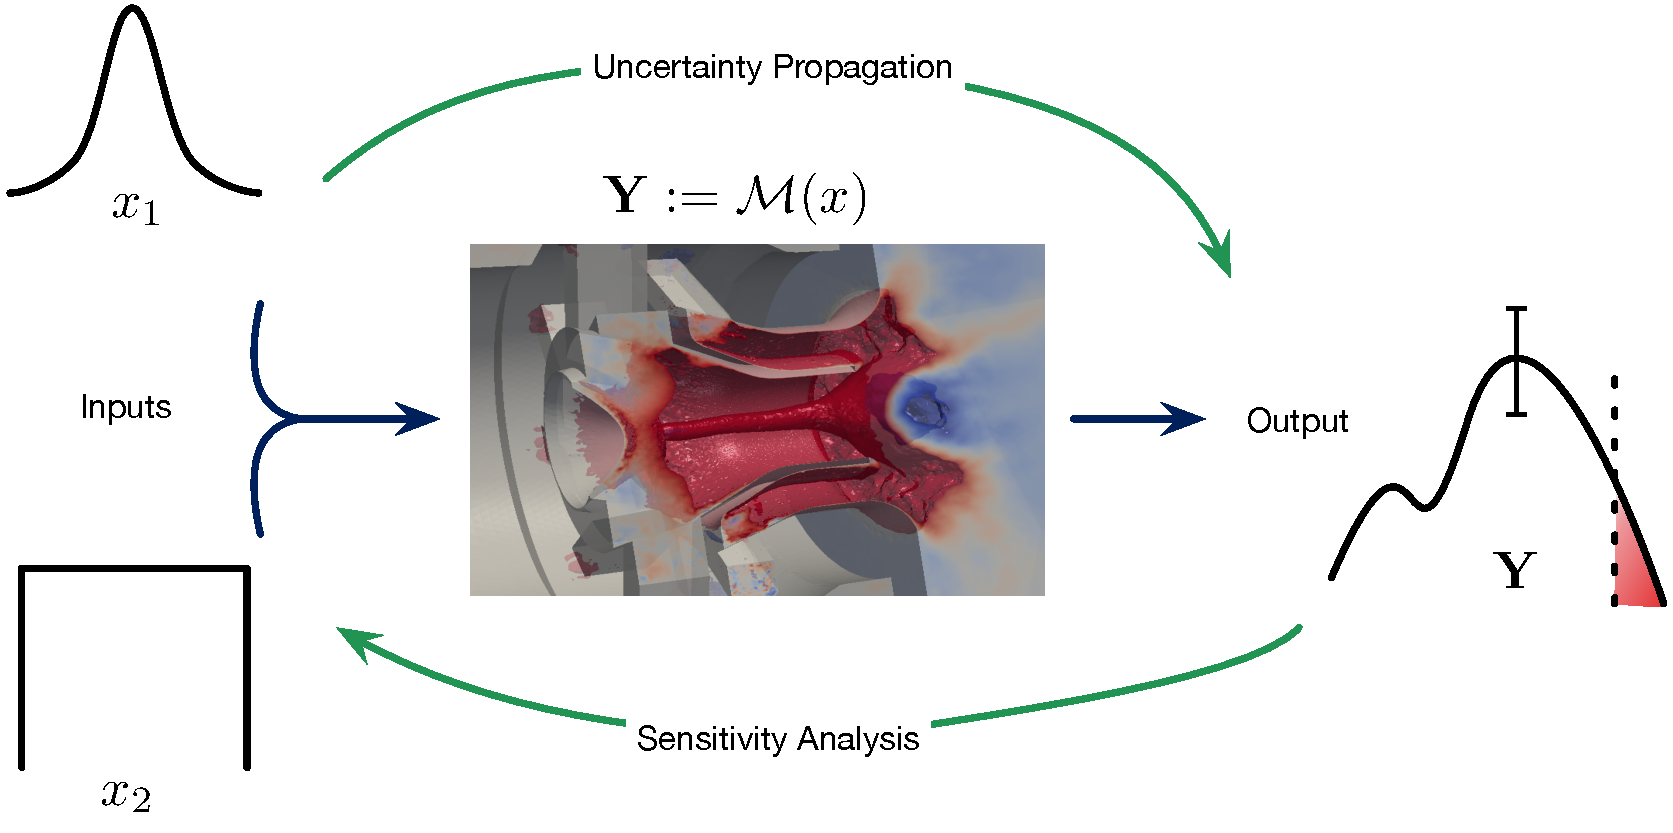
\includegraphics[width=\linewidth,keepaspectratio]{fig/literature/schema_UQ.pdf}
\caption{Schematization of the Uncertainty Quantification procedure in case of two uncertain input parameters perturbing a numerical model $\mathcal{M}$.}
\label{fig:context}
\end{figure}

The output variability of a system can be confusing regarding the source of these uncertainties. Does it come from our model or from the physics? Uncertainties can be classified as:

\begin{description}
	\item [Aleatoric errors:] intrinsic to the system,
	\item [Epistemic errors:] due to a lack of knowledge,%. We can reduce it by improving our model or adding experiments,
	\item [Numerical error:] due to the construction of the numerical scheme.
\end{description}

Ideally, our model should only contain aleatoric uncertainties as it represents the physical variability of the system. However, the diversity of uncertainties due to the boundary conditions or initial conditions as well as to model parameters (input data, geometry, simplification of the model physics, etc.) limits the predictivity of the simulations: the QoI can be easily affected and shadowed by the conjugation of all these types of uncertainties. This assessment explains why Uncertainty Quantification (UQ) is now becoming a mandatory step in application-oriented modelling for operational and industrial purposes~\cite{degennaro2015,masquelet2017}. It provides insight into the level of uncertainty in the numerical simulation results but also gives access to a sensitivity analysis which aims to describe the respective influences of the input parameters on the QoI. The inclusion of UQ in a design optimization cycle hence allows manufacturers to design quicker and obtain better, cheaper and more robust products. Depending on the question we seek to answer, we have to determine the type of UQ study to perform:

\begin{itemize}
	\item \emph{Uncertainty Propagation,}\hfill\\
Propagate an initial perturbation within the system and observe its outputs.
	\item \emph{Sensitivity Analysis,}\hfill\\
Rank the input parameters regarding their impact on the output.
	\item \emph{Risk Assessment.}\hfill\\
Observe the probability to exceed a threshold or get the probability of a particular quantile.
\end{itemize}

Each question is answered using specific tools and special care has to be taken if on wants to conduce different analysis. For instance, some formulations to compute sensitivity indices have requirements which are not conform with both Uncertainty Propagation and Risk Assessment.

Classical UQ methods, based on the \emph{Monte-Carlo} approach, require a large number of simulations~\cite{Saltelli2007}, which quickly go beyond the limits of available resources (such as CPU, financial costs). This is especially true when it comes to large-dimensional problems, both with respect to the domain discretization and to the number of uncertain input parameters. The cost of the UQ study can, however, be significantly reduced when the experiment is replaced by a proxy, or surrogate model, which is formulated in a parameter space and which is fast to evaluate for any set of uncertain variables~\cite{martin2005}. The construction of the surrogate model requires a set of experiments, Design of Experiments (DoE), to learn from. To correctly emulate the real experiment, the definition of the DoE is paramount.\bigskip

%\begin{quotation}
%
%The purpose of this thesis is to propose directions of improvement on various methodological aspects of UQ applied to costly numerical environments. The methods developed can be used in various fields and are demonstrated through multiple applications. Moreover, these methods are not limited to the use of numerical experiments and can be used equally for \emph{in vivo} experiments.
%
%%{\fontfamily{FiraCode-Light}\selectfont The purpose of this thesis is to propose directions of improvement on various methodological aspects of UQ applied to costly numerical environments. The methods developed can be used in various fields and are demonstrated through multiple applications. Moreover, these methods are not limited to the use of numerical experiments and can be used equally for \emph{in vivo experiments.}
%
%\end{quotation}

\begin{warningbox}
The purpose of this thesis is to propose directions of improvement on various methodological aspects of UQ applied to costly numerical environments. The methods developed can be used in various fields and are demonstrated through multiple applications. Moreover, these methods are not limited to the use of numerical experiments and can be used equally for \emph{in vivo} experiments.	
\end{warningbox}


%\newpage

\section*{Organization}
%\addcontentsline{toc}{section}{}

This manuscript is divided into four parts and is tailored as follows: 

\begin{description}
	\item[\Cref{part:intro}] \emph{After a general introduction about the context of this thesis,  \cref{chap:review} reviews the literature on concepts and methods for UQ,}\hfill\\
\Cref{sec:doe} goes from a state-of-the-art on the different methods to design experiments; then \cref{sec:uq} describes the different techniques commonly used in UQ, as well as the latest advances. \Cref{sec:surrogate} details the construction of a surrogate model which may be required to perform such statistical analysis. \Cref{sec:visu} presents how uncertainties are commonly visualized. After this literature review, some scientific questions arise and the complete scope of this thesis work is given in~\cref{chap:questions}.

	\item[\Cref{part:contributions}] \emph{presents my methodological contributions,}\hfill\\
In~\cref{chap:batman}, a new UQ open-source tool is introduced. It serves as a demonstrator for all the methods developed. Following chapters are the responses to the scientific questions rose. \Cref{chap:doe} introduces a new iterative and versatile sampling method while \cref{chap:resample} addresses question of the resampling of an existing DoE. Finally, \cref{chap:visu} proposes novel visualization techniques to visualize uncertainty in high dimensions.

	\item[\Cref{part:applications}] \emph{some applications of the new methods---in a costly numerical environment---are proposed,}\hfill\\
%	through~\cref{chap:mascaret,chap:ls89,chap:swirler,chap:optim,chap:psaap},}\hfill\\
\Cref{chap:mascaret} is a comparison between two surrogate models. \Cref{chap:ls89} demonstrates the new resampling techniques capabilities, to perform the first UQ analysis using Large Eddy Simulation on the LS89 blade cascade. \Cref{chap:swirler,chap:optim} present two applicative cases of Batman. In~\cref{chap:swirler}, the focus is put on the dimensionality of the input parameter space while in~\cref{chap:optim}, the toolchain is used to perform and UQ analysis to understand the physical phenomena and to perform an optimization of the parameters. %\Cref{chap:psaap} briefly introduces a work in progress where the new sampling method is being used.

	\item[\Cref{part:conclusion}] \emph{put a point on this thesis work and draw some perspectives for future work.}
\end{description}


\chapter{Literature Review}\label{chap:review}

\begin{chapquote}
Ce chapitre présente une revue de la littérature sur les concepts et les méthodes associées à la quantification des incertitudes (UQ) dans un environnement numérique coûteux : de la définition d'un plan d'expériences (DoE) pour construire un modèle de substitution, à l'utilisation de ce modèle de substitution pour calculer les statistiques et finalement visualiser les résultats.

Les avancées et les limites actuelles du DoE sont présentées~\cref{sec:doe}. Les séquences OLHS et \emph{Sobol'} sont toutes deux considérées comme des pratiques de référence bien qu'elles présentent certaines limites telles que les propriétés itératives et la randomisation, respectivement.

En utilisant cet échantillon, on peut effectuer une analyse UQ avec des méthodes détaillées~\cref{sec:uq}. L'analyse de sensibilité globale (GSA) est recommandée par rapport à une analyse locale de sensibilité. Concernant les méthodes à proprement dit, une SA basée sur la variance reste prédominante, mais les méthodes basées sur les moments semblent être un bon complément dans une étude. Dans un environnement numérique coûteux, il n'est pas possible d'effectuer directement une UQ et l'utilisation d'un modèle de substitution offre une solution. \Cref{sec:surrogate} expose deux des méthodes les plus utilisées : Processus gaussien (GP) et Chaos polynomial (PC). Enfin, \cref{sec:visu} introduit le problème de la visualisation des incertitudes. Il s'agit d'un domaine relativement nouveau avec un corpus d'études limité. Il n'y a actuellement aucune recommandation claire sur la façon de visualiser les incertitudes. À partir de cette revue, \cref{chap:questions} détaille les trois questions auxquelles cette thèse vise à répondre :
\begin{itemize}
\item Comment construire un DoE dans un espace de paramètres à haute dimension ?
\item Comment rééchantillonner un DoE en considérant la QoI d'expériences déjà évaluées ?
\item Comment visualiser les incertitudes dans des cas de grande dimension ?
\end{itemize}

\end{chapquote}

\section{Design of Experiments}\label{sec:doe}

\lettrine{O}{ne} of the main objectives when performing numerical---or real---experiments is to understand the variation of a QoI with respect to the variation of some input parameters~\citep{Sacks1989}. Each experiment, or sample, corresponds to a particular set of input parameters $x_k$ with $k \in [1, \dots , d]$, where $d$ is the number of dimensions. As a result, the group of $N_s$ samples, or DoE, is noted as $\mathbf{X}^{N_s}_d$. For simplicity either the dimensionality $d$ or the number of samples $N_s$ is omitted in the manuscript. Nevertheless, the subscript denotes $d$ while the superscript denotes $N_s$. Then the forward model (or experiment) $\mathcal{M}$ can be simulated for each sample
\begin{align}
(\mathbf{X}^{N_s}_d, \mathcal{Y})=\left(\mathbf{x}^{(i)},\mathbf{Y}^{(i)}\right)_{1\leq i\leq N_{s}},
\end{align}
\noindent where $\mathcal{Y}$ is the QoI and $\mathbf{Y}^{(i)} := \mathcal{M}(\mathbf{x}^{(i)})$ corresponds to the deterministic integration of the forward model $\mathcal{M}$ as a black box for the $i$th set of input parameters $\mathbf{x}^{(i)}$---see~\cref{fig:doe}.

\begin{figure}[!ht]
\centering
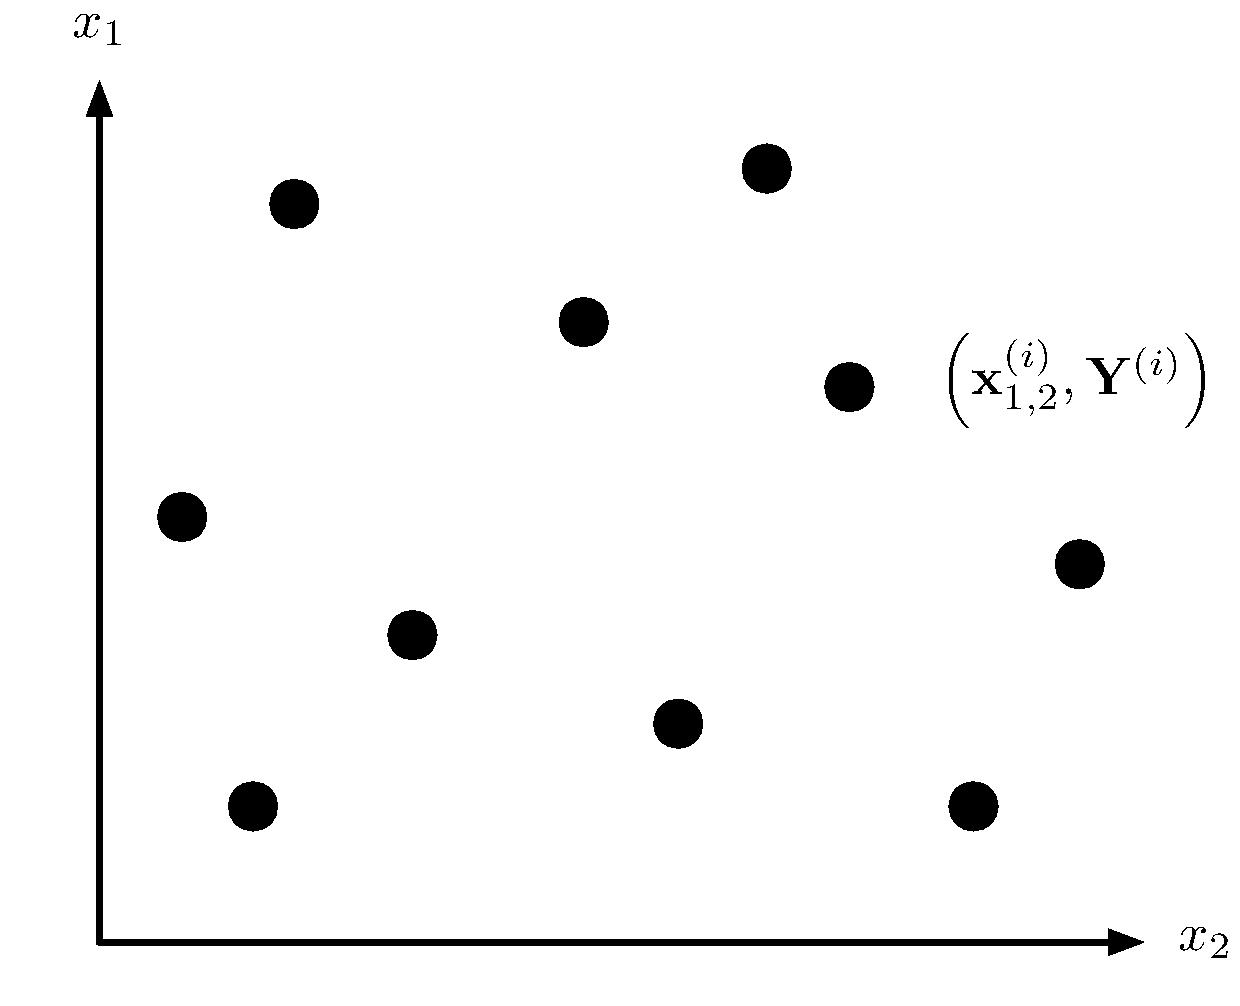
\includegraphics[width=0.5\linewidth,keepaspectratio]{fig/literature/doe.pdf}
\caption{Sketch of a 2-dimensional Design of Experiments. Every \emph{black dot} represents an experiment $x_{1, 2}^i$ used to compute the output $\mathbf{Y}^{(i)}$.}
\label{fig:doe}
\end{figure}

In its basis form, a DoE is described by a $d$-dimensional cube: a hypercube---see~\cref{fig:sketch_hypercube}. A hypercube is parametrized by the minimal and maximal values of each parameter. If parameters depends on each other, or if there are constrains on the parameters, non-rectangular domains~\citep{Lekivetz2015} have to be considered.

\begin{figure}[!ht]
\centering
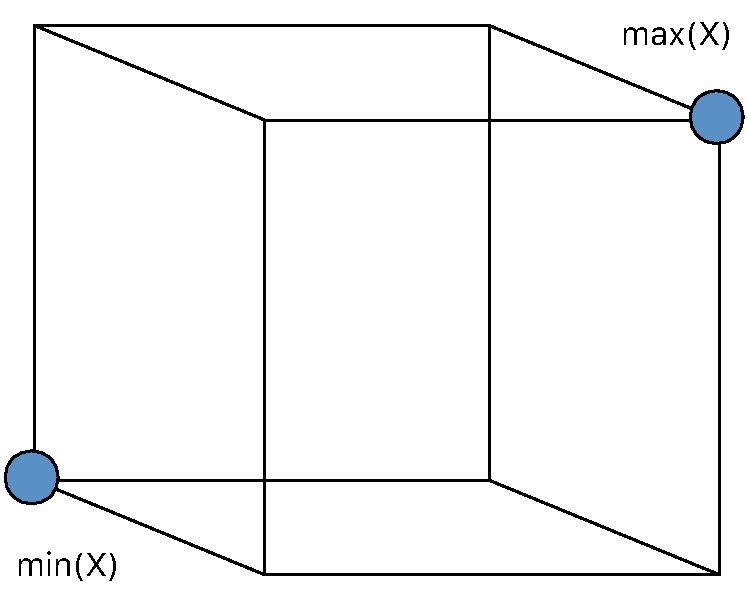
\includegraphics[width=0.5\linewidth,keepaspectratio]{fig/literature/hypercube.pdf}
\caption{Sketch of a 3-dimensional hypercube.}
\label{fig:sketch_hypercube}
\end{figure}

From exploratory phases to more advanced analyses, such as UQ and robust optimization, DoE aims at helping better understand the physical mechanisms governing the problem of interest~\citep{Saltelli2007}. Therefore, the objective of efficient DoE is to maximize the coverage of the input space, i.e. space filling, with the aspiration of capturing most of the underlying physics. Such analyses typically require a large number of experiments in order for the statistics of the QoIs to converge (especially for extreme quantiles). However, depending the complexity of the experiment, its intrinsic cost or its return time, the total number of experiments may be limited. In this regard, many studies have focused on the optimization of the space-filling properties for a given number of experiments.

Beyond random design also called \emph{Monte Carlo} experiments, One-At-a-Time (OAT) design is the most trivial form of engineered DoE. It consists in changing only one parameter at a time. While this method is simple to implement and allow for a quick interpretation on a physical aspect, this sampling procedure requires a huge number of simulation as requiring $(N_s)^d$ samples. This exponential growth is called the \emph{curse-of-dimensionality}. Let's consider the unit-hypercube, all bounds range from 0 to 1. Now, having a distance of 0.1 between each point, the number of points required to fill the unit interval would be 10. In a 2-dimensional hypercube the same spacing would require 100 and in 3-dimensions 1000 points. As the number of dimensions goes, the number of experiments which is required to fill the space evenly rises exponentially as the volume of the space increases---see~\cref{fig:curse_dim}. To mitigate this problem, one could sparse the DoE. The problem comes to an assessment of the quality of this DoE.

\begin{figure}[!ht]
\centering
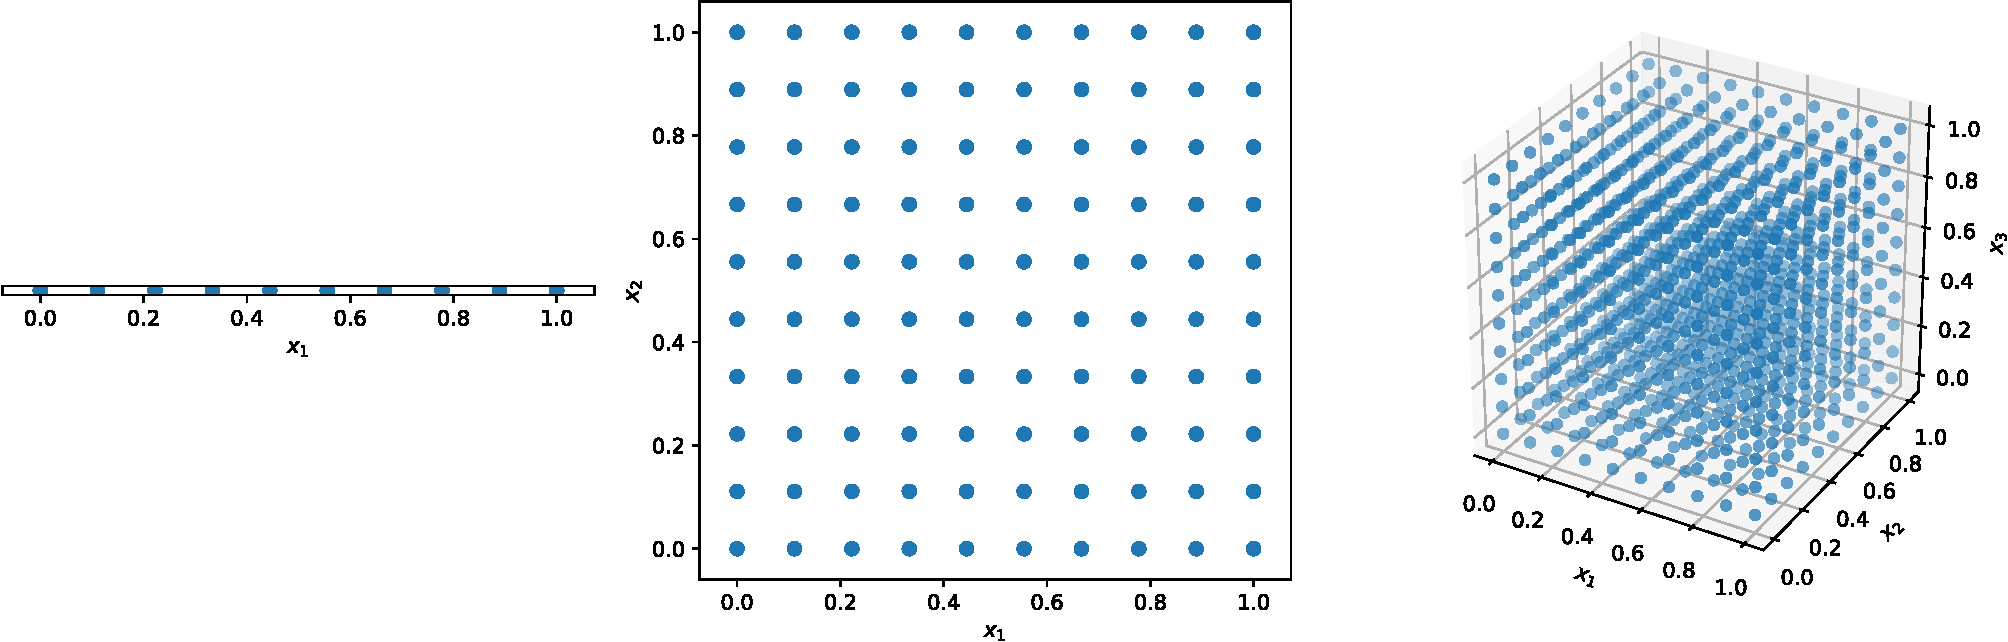
\includegraphics[width=\linewidth,keepaspectratio]{fig/literature/curse_dim.pdf}
\caption{Sketch of the \emph{curse-of-dimensionality}. Visualization of the volume of the parameter space in 1, 2 and 3 dimensions. OAT design with points separated by a distance of 0.1.}
\label{fig:curse_dim}
\end{figure}

Different metrics are commonly used to assess the space filling of a DoE. They can be categorized into \emph{(i)} geometrical and \emph{(ii)} uniformity criteria. Among the most used geometrical criteria are the \emph{maximin} and \emph{minimax}~\citep{Pronzato2017}. They, respectively, maximize the minimal distance between all points or minimize the maximal distance between any location in space and all points of the sample. A similar criterion is found by using a \emph{minimum spanning tree}~\citep{Franco2009} in which the best design corresponds to a maximization of the mean distance between all connections and the minimization of the variance in these distances. The uniformity criterion, instead, measures how the spread of the points deviates from a uniform distribution. The centred discrepancy $C^2$ is commonly used to measure the uniformity~\citep{Fang2006,Damblin2013}:
\begin{align}
C^2(\mathbf{X}^{N_s}_d) =& \left( \frac{13}{12} \right)^d - \frac{2}{N_s}\displaystyle\sum_{i=1}^{N_s}\prod_{k=1}^{d} \left( 1 + \frac{1}{2} \mid  x_k^{(i)} - 0.5\mid - \frac{1}{2} \mid  x_k^{(i)} - 0.5\mid^2\right)\\ \nonumber
& + \frac{1}{N_s^2}\sum_{i,j=1}^{N_s}\prod_{k=1}^d \left( 1 + \frac{1}{2} \mid  x_k^{(i)} - 0.5\mid + \frac{1}{2} \mid  x_k^{(j)} - 0.5\mid - \frac{1}{2} \mid  x_k^{(i)} - x_k^{(j)}\mid \right). \label{eq:c2}
\end{align}

There are three main methodologies for defining a DoE: \emph{(i)} MC, \emph{(ii)} \emph{Latin Hypercube Sampling} (LHS) and \emph{(ii)} Quasi-\emph{Monte Carlo} (QMC) methods~\citep{Cavazzuti2013,Garud2017}. Kucherenko \emph{et al.}~\citep{Kucherenko2015} have recently compared MC and LHS against the low discrepancy sequence of \emph{Sobol'}, which is a well-established QMC method. They concluded that both LHS and QMC offer superior integration performance over MC. Integrating a complexe function requires a good space coverage and this performance is assimilable to a discrepancy measure. \Cref{fig:ex_doe} is an example of these three methods to construct samples of size $N_s = 256$ in dimension $d = 2$. In this low dimensional space, the superiority in terms of space coverage of both LHS and \emph{Sobol'} over MC is clear. MC exhibits lots of clustered regions and it translates in a two orders difference in terms of centred discrepancy compared to the other methods.

\begin{figure}[!ht]
\centering
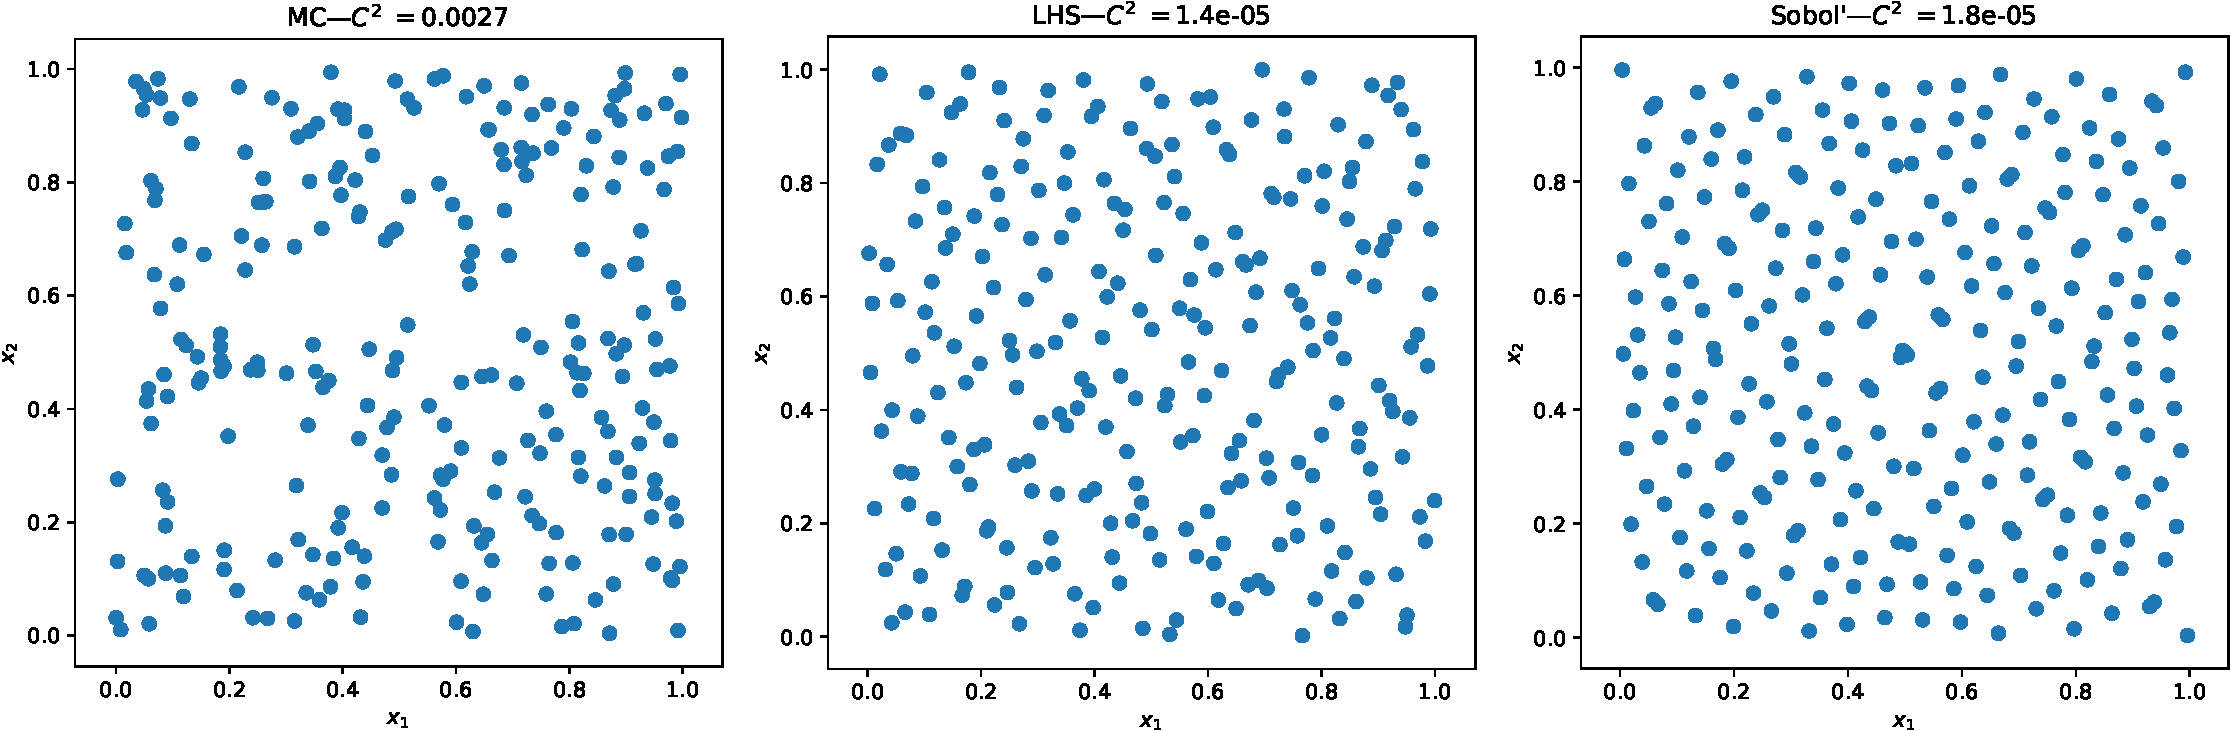
\includegraphics[width=\linewidth,keepaspectratio]{fig/literature/doe_examples.pdf}
\caption{Example of DoE constructed with MC, LHS and the low discrepancy sequence of \emph{Sobol'}  with $N_s=256$.}
\label{fig:ex_doe}
\end{figure}

On the one hand, LHS-based sampling methods are one-shot design strategies~\citep{Mckay1979,Fang2006}. The principle is simple: considering $N_s$ samples, in each 1-dimensional subprojection of the parameter space there should be $N_s$ samples. It means that samples are not sharing coordinates with each other. Orthogonal arrays are a slight evolution of this principle. Each 1-dimensional subprojection is spitted into $N_s$ to form an orthogonal grid of size $N_s^d$ and only one sample is allowed per cell. \Cref{fig:lhs} shows two different orthogonal LHS with $N_s=10$. Although both valid, they do not cover the parameter space equally. In~\cref{fig:lhs}(b) lots of points are aligned preventing some regions to be explored. Constructing such design is numerically easy and it is possible to optimize the space-filling properties by swapping elements for instance~\cite{Fang2006,Damblin2013}. A basin-hopping algorithm~\cite{wales1997} is commonly used to resolve this global optimization problem. This is a stochastic algorithm used to find global optima which combine a random perturbation of the parameters, a local minimization and an accepting or rejecting of new coordinates depending on a decaying parameter.

\begin{figure}[!ht]               
\centering
\subfloat[]{
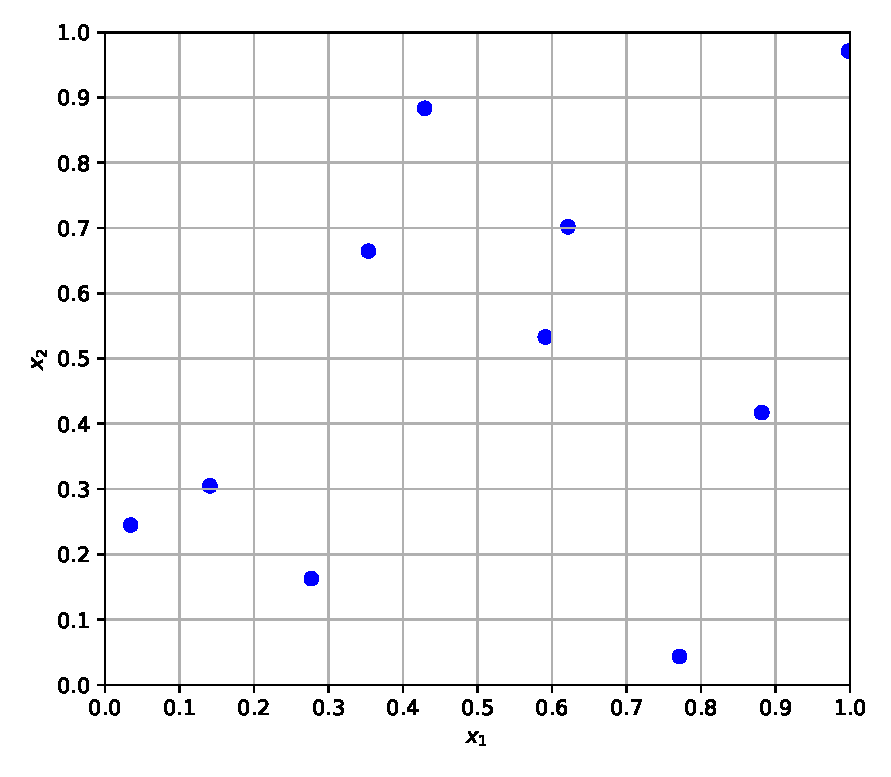
\includegraphics[width=0.47\linewidth,height=\textheight,keepaspectratio]{fig/literature/lhs_ok.pdf}}
 ~       
\subfloat[]{
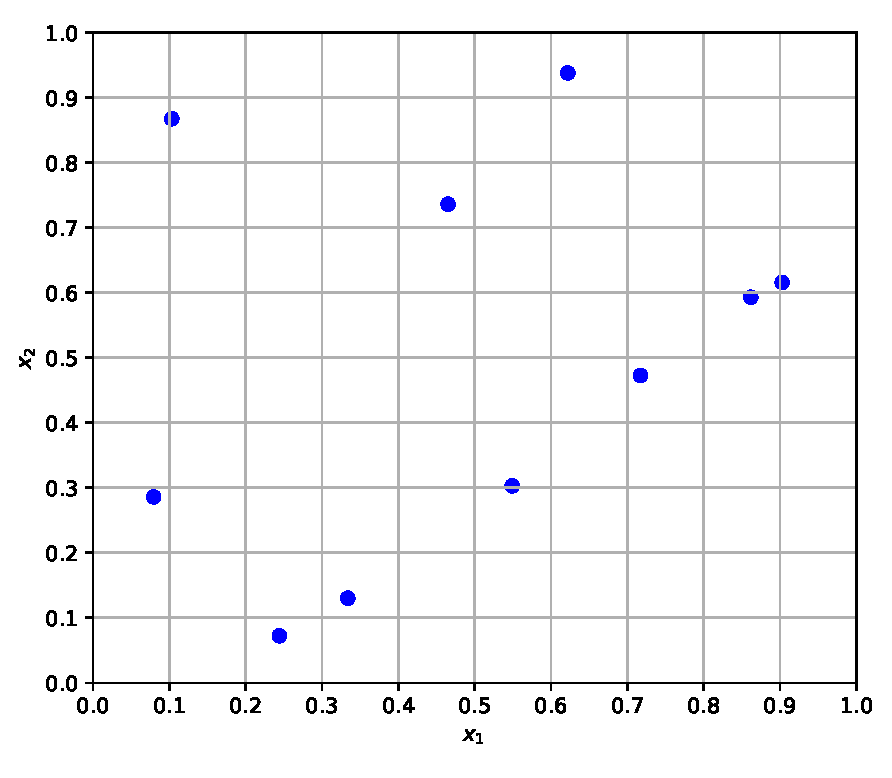
\includegraphics[width=0.47\linewidth,height=\textheight,keepaspectratio]{fig/literature/lhs_ko.pdf}}
\caption{Two orthogonal LHS examples with $N_s =10$ demonstrating the qualitative difference in terms of space-filling.}
\label{fig:lhs}
\end{figure}

\noindent The use of LHS requires the practitioner to set \emph{a priori} the total number of samples contained in the DoE. Although there have been some attempts to construct progressive LHS, they still require an initial design to work properly~\citep{Sheikholeslami2017}.

On the other hand, low discrepancy sequences are iterative designs which can be continued without compromising the discrepancy. The practitioner is then able to increase the number of samples afterwards for quality reasons or if other experiments can be afforded. 

\citet{Liu2018} recently reviewed iterative DoE in a metamodeling context. In their study, it is shown that most iterative methods need an initial design as a starting point. A particular benefit of this approach is that it allows the use of physics information from the system to guide further exploration of the DoE. In this case, such iterative methods are called adaptive methods. Here as well, basin-hopping-based methods are commonly used to find the coordinates of the new sample. Except for some work in~\citep{Crombecq2011}, the number of iterative methods not requiring an initial design is limited. This can be explained both by the quality of the initial designs (using LHS of \emph{Sobol'} sequence) and by the performance of the refinement algorithm. There are even fewer options if the iterative design cannot take advantage of the output of the experiments. Low discrepancy sequences are an example of such methods. In some context, stochastic methods may be required ---\thinspace to compute sensitivity indices for instance~\citep{Saltelli2010}. Scrambling the sequences~\citep{Owen1998} can avoid this pitfall but then the method is no longer iterative.

\section{Uncertainty Quantification}\label{sec:uq}

\subsection{Uncertainty Propagation}\label{sec:up}
\lettrine{U}{ncertainty Propagation} (UP) seeks to transmit uncertainties throughout the system. But are we talking about the uncertainties of the input parameters or the output QoI? In this section we focus on a \emph{direct problem} which relate to the transmission of uncertainties from the input to the output. The other way around is called an \emph{inverse problem} and is discussed in~\cref{sec:sa}.

Uncertainties can be described using a probabilistic approach through the use of Probability Density Functions (PDF). This function computes the probability of occurrence of a phenomenon. Thus, propagating uncertainties comes to determining the PDF of the QoI.

\begin{figure}[!ht]
\centering
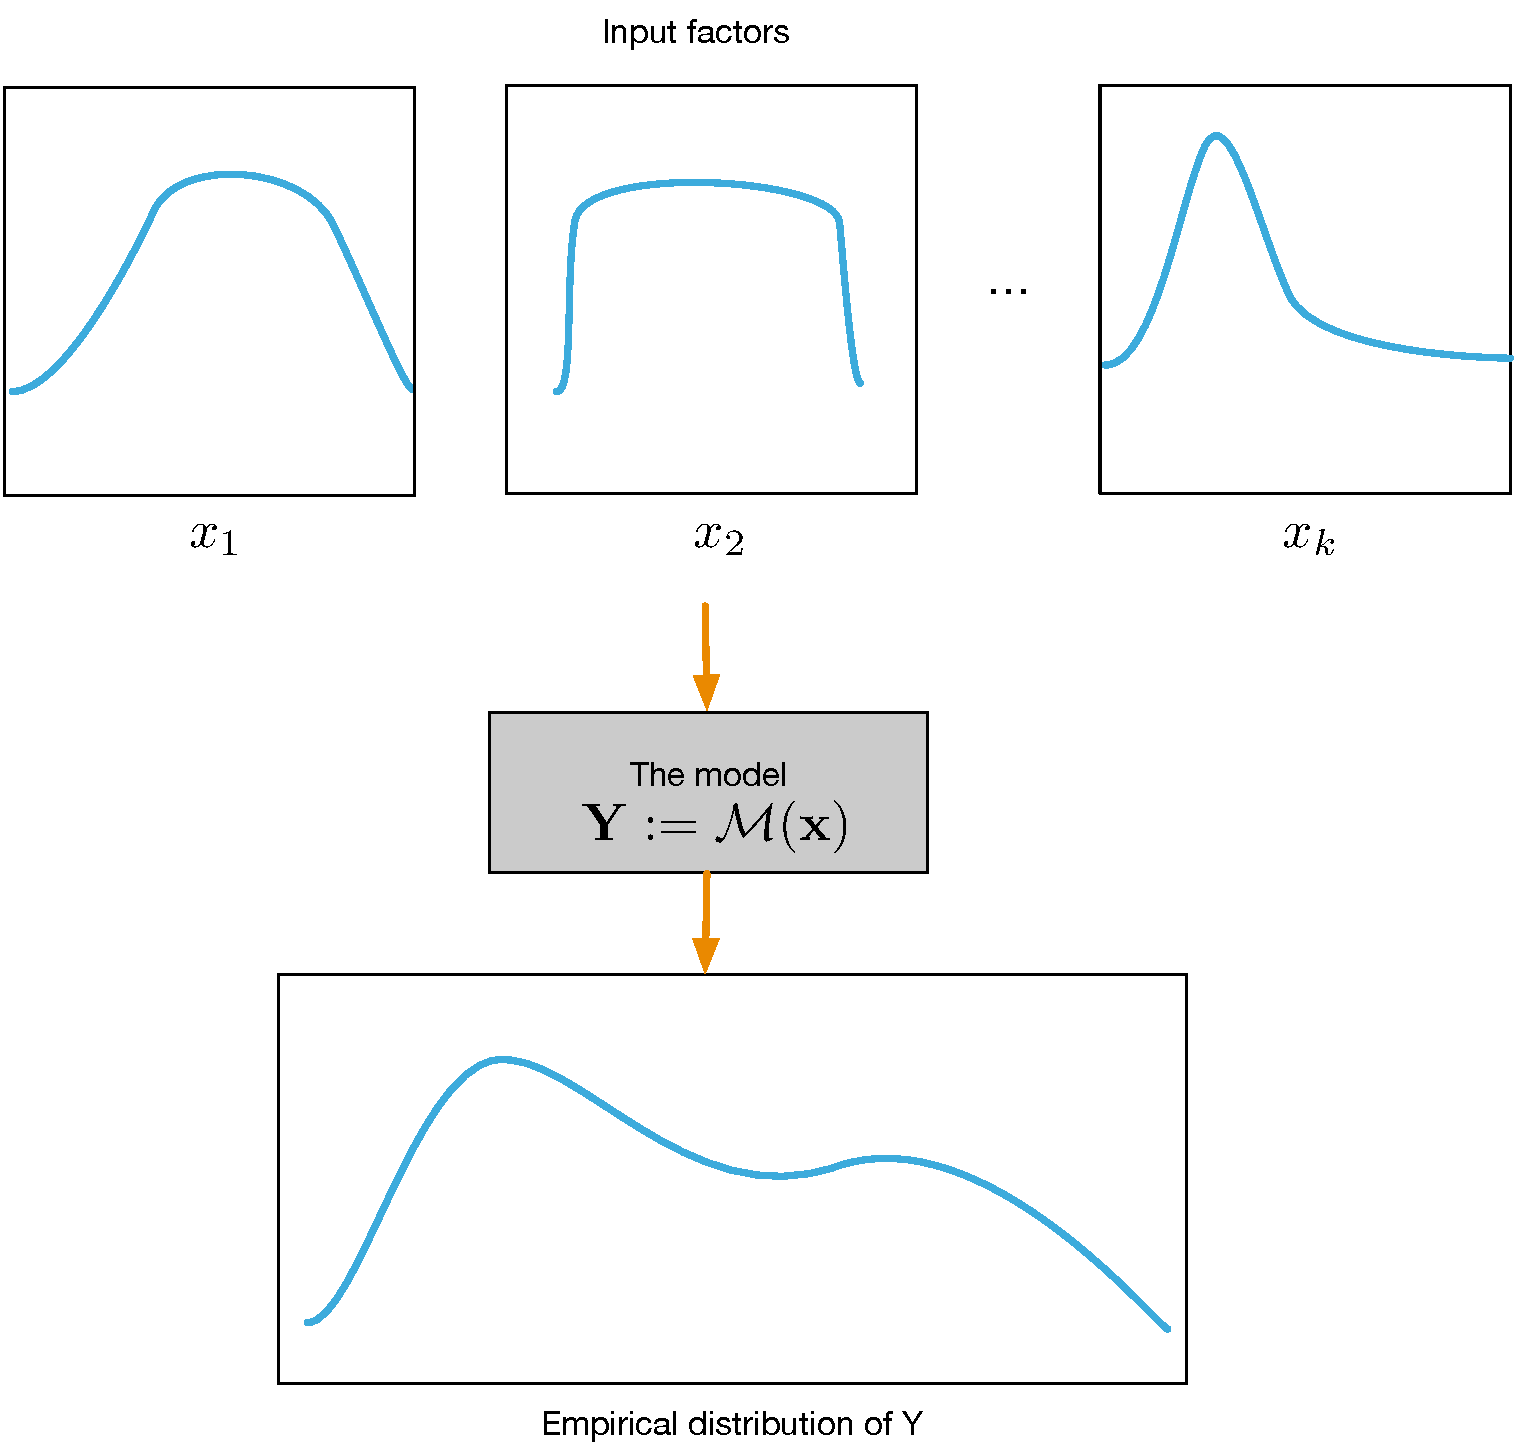
\includegraphics[width=0.7\linewidth,keepaspectratio]{fig/literature/propagation.pdf}
\caption{Sketch of the UP procedure.}
\label{fig:UP}
\end{figure}

\Cref{fig:UP} is a representation of the UP procedure. In practice, propagating uncertainties comes to sampling the PDFs of inputs and observing the impact on the QoI. It should be emphasized that the outcome of the UP \emph{depends} on the prescribed PDFs for the inputs. The nature of the PDF and the ranges of each parameter is paramount. Without any prior knowledge on input parameters, uniform distributions are traditionally used. As for the ranges, some fixed percentage of variation is commonly used. While this strategy could indeed correspond to the correct variability of some parameters, this may lead to wrong analysis. In~\citep{pilkey}, the example of radioactive waste transport on the Yucca Mountain is taken. In this UP analysis, the percolation rate of the water from the surface to the disposal was wrongly estimated between 0.02 and 1 millimetre per year while its true value was close to $\sim \unit{\numprint{3000}}{\milli\metre}$. The underestimation of this parameter led to an underestimation of 4 orders of magnitude of the transport of some radioactive component.

As we are interested in computing statistics on the QoI, this requires a statistically significant sampling. A high number of samples is required to recover the empirical PDF of the QoI. One must note that in order to find the tail of the PDF---the least frequent event---it requires an even larger number of samples.

Discrete representations such as histograms can be used to represent the PDF. However, continuous functions can be obtained using a technique called Kernel Density Estimation (KDE)~\cite{Wand1995}. The probability to observe a QoI's value $Y^*$ is given by the PDF estimator $\hat{f}(Y^*)$
\begin{align}
\hat{f}(Y^*)&= \frac{1}{N_{s}}\sum_{i=1}^{N_{s}} K_{h_i}(Y^*-Y^{(i)}),
\end{align}
\noindent where $N_s$ is the number of samples. $K_{h_i}(.) = K(./h_i)/h_i$ is the scaled kernel chosen for the modal probability density function with $h_{i}$ the bandwidth for the \emph{i}th component. In the present work $K$ is the Gaussian kernel and $h_{i}$ are optimized by cross-validation of the log-likelihood of the data. It reads
\begin{align}
K\left(Y^*,Y^{(i)}\right) = \exp\left( - \frac{D\left(Y^*,Y^{(i)}\right)^2}{2h^2} \right), \label{eq:kde}
\end{align}
\noindent with $D$ a distance function. Having a Gaussian kernel does not restrict the estimated PDF to be Gaussian and this should not be mistaken. It should be noted that estimating the density in a high-dimensional parameter space is challenging~\citep{Scholkopf1999,Scott2015}. See \cref{sec:visu} for a $n$-dimensional representation of the PDF.

Depending on the number of samples available and on the parameters of the method, this process can lead to a PDF which is far from the real one. The principle of KDE is fairly easy to understand---see~\cref{fig:kde}. Each sample value $Y$ is represented on the $x$-axis. Around each value, a rectangle of fixed width and fixed height is drawn. When there is an overlap, the rectangle values are summed up. The value of the width represents the bandwidth, and the general shape of the \emph{rectangle} is called the kernel. As previously stated, Gaussian kernel is classically used and corresponds to a bell-curve shape. From this procedure, it can be seen that the resulting PDF can be of any shape and is not limited to the nature of the kernel. In a sense, the kernel act as a filtering artefact.

\begin{figure}[!ht]
\centering
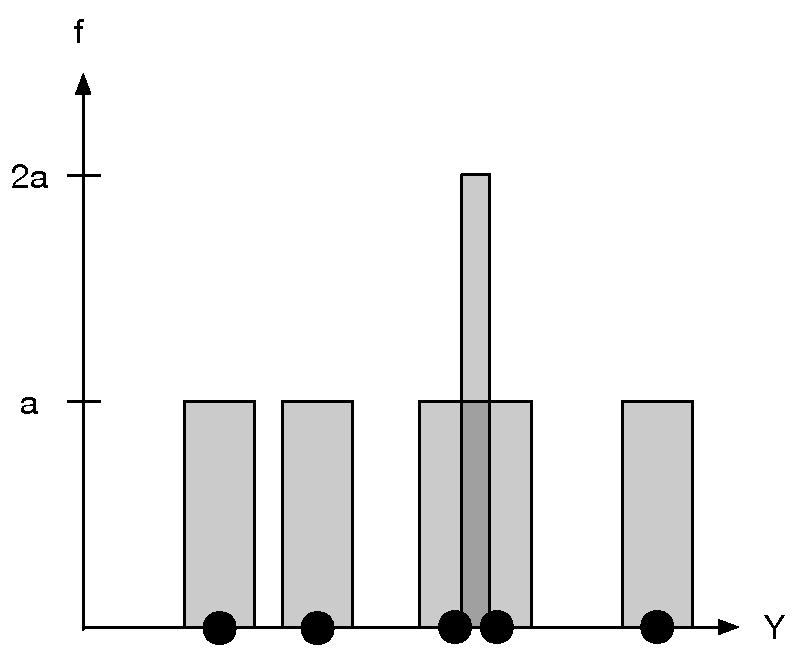
\includegraphics[width=0.6\linewidth,keepaspectratio]{fig/literature/kde.pdf}
\caption{Sketch of a Kernel Density Estimation procedure with a rectangular kernel.}
\label{fig:kde}
\end{figure}

\Cref{fig:ex_pdf}(a) presents a KDE of a 1-dimensional QoI along with a histogram representation of the data. The KDE acts as a smoothing procedure of the histogram as previously highlighted. Another possibility---\cref{fig:ex_pdf}(b)---is to use the quantile dotplot \cite{kay2016} which allows to directly count the quantiles. In this example, there are 20 circles, and below $F=22.5$ there are 11 circles. Thus >50\% of the samples are located below $F=22.5$.

\begin{figure}[!ht]               
\centering
\subfloat[Kernel Density Estimation and histogram]{
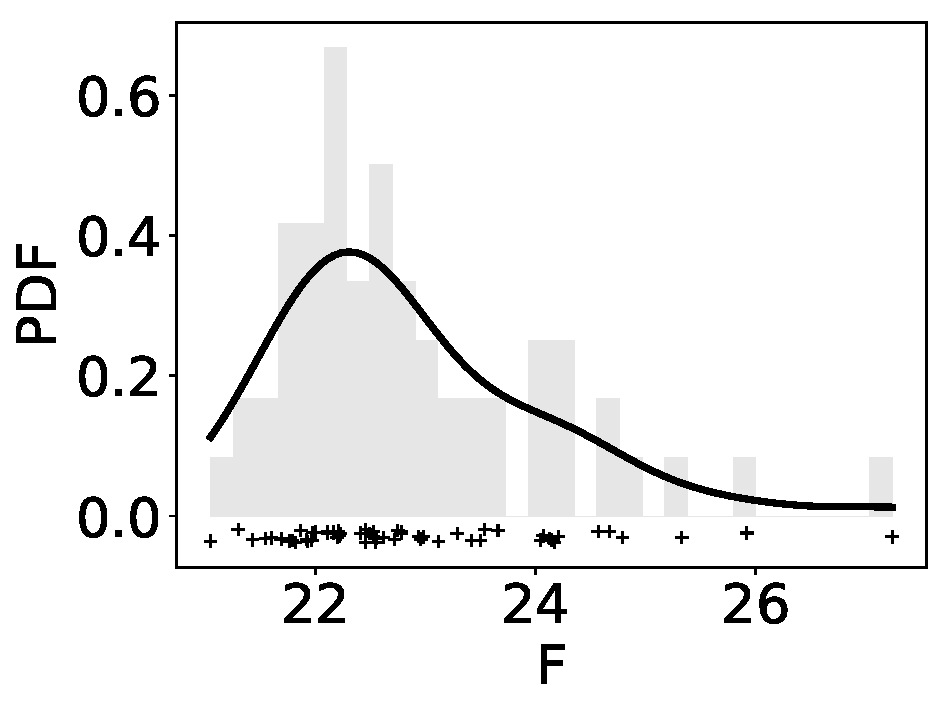
\includegraphics[width=0.47\linewidth,height=\textheight,keepaspectratio]{fig/literature/pdf_hist.pdf}}
 ~       
\subfloat[Kernel Density Estimation and quantile dotplot]{
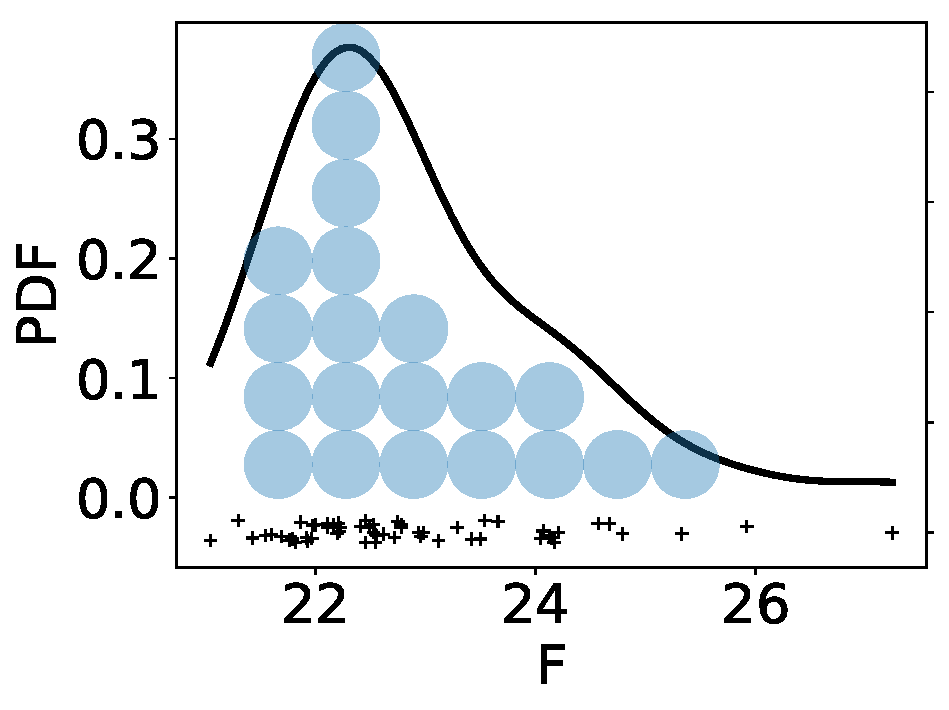
\includegraphics[width=0.47\linewidth,height=\textheight,keepaspectratio]{fig/literature/pdf_dotplot.pdf}}
\caption{Visualization of a 1-dimensional PDF.}
\label{fig:ex_pdf}
\end{figure}

Once the PDF of the QoI is available, it can be used to: \emph{(i)} observe the probability of exceeding a threshold; \emph{(ii)} compute the probability to have a certain event; or just \emph{(iii)} get general statistics (mean, variance, quantiles).

\subsection{Sensitivity Analysis}\label{sec:sa}
\lettrine{S}{ensitivity Analysis} (SA) refers to the determination of the contribution of different parameters on quantities of interest~\cite{Saltelli2007,iooss2016}. The most natural way to do SA would be to consider the derivatives. But this information is known to be too local or restrictive---although there are some works extending the capabilities of these methods~\cite{kucherenko2016}. In the literature, a distinction is made between local and global SA. In the following both local-based SA (derivative) and global-based SA (variance-based and moments-based) methods are presented.

\subsubsection{From Local to Global Sensitivity Analysis}

An intuitive way to characterize the importance of each parameter on a QoI is to compute the derivatives of the output with respect to an input. This method is called \emph{elementary effects} and a successful implementation is found with \citet{morris1991}. An elementary effect $d\mathbf{x}_{k}^*$ is defined as
\begin{align}
d\mathbf{x}_{k}^* = \frac{ \mid Y(\mathbf{x}_{k}^*) -  Y(\mathbf{x}_{k}) \mid}{\mid \mathbf{x}_{k}^* - \mathbf{x}_{k}  \mid},
\end{align}
\noindent with $\mathbf{x}_{k}$ a given sample and $\mathbf{x}_{k}^*$ a sample which differs from $\mathbf{x}_{k}$ by an increment $\delta$. This effect can be computed with respect to $N_s$ samples and $d$ dimensions which induce to a total number of samples $N = N_s\times(d + 1)$. It is called a screening method and it corresponds to an OAT walk of the DoE. \Cref{fig:morris} is an example with $N_s = 5, d = 3$. Then the mean of absolute elementary effects reads
\begin{align}
\hat{\mu_k} = \frac{1}{N_s} \sum_{i=1}^{N_s} \frac{ \mid Y(\mathbf{x}_{k}^*) -  Y(\mathbf{x}_{k}^i) \mid}{\mid \mathbf{x}_{k}^* - \mathbf{x}_{k}^i  \mid}.
\end{align}

\begin{figure}[!ht]
\centering
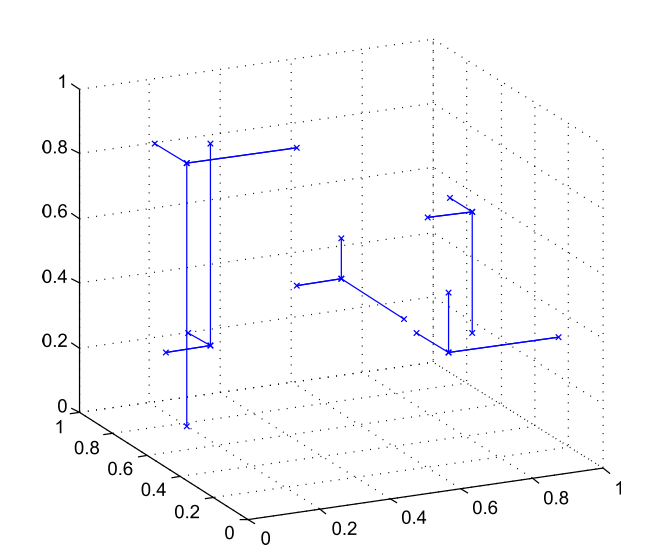
\includegraphics[width=0.8\linewidth,keepaspectratio]{fig/literature/morris.png}
\caption{Sketch of \emph{Morris}'s screening method. Source~\cite{Becker2018}.}
\label{fig:morris}
\end{figure}

A popular extension of this method is found with the derivative-based global sensitivity measures (DGSM)~\cite{kucherenko2016,Becker2018}. Although these methods perform well in high dimensions and with a low sampling size, they are not exempt of flaws. As local methods, the construction of the indices is based on local OAT variations which are not able to take into account correctly correlations between the input parameters. 

It should be noted that some solver directly give access to the derivative information for each sample for a reduced extra cost. Although this capability requires some effort in terms of code, some automatic derivative software can alleviate this effort.

\subsubsection{Variance-Based Sensitivity Analysis}
Variance-based Sensitivity Analysis allows obtaining the contribution of the parameters on the QoI's variance~\cite{ferretti2016}. Here, classical \textit{Sobol'}~\cite{Sobol1993} method is presented which gives not only a ranking but also quantifies the importance factor using the variance. This method makes the hypothesis of the independence of the input variables. It uses a functional decomposition of the variance of the function to explore
\begin{align}
\mathbb{V}(Y) &= \sum_{i}^{d} \mathbb{V}_i (Y) + \sum_{i<j}^{d}\mathbb{V}_{ij}(Y) + ... + \mathbb{V}_{1,2,...,d}(Y),
\end{align}
\noindent introducing conditional variances:
\begin{align}
\mathbb{V}_i(Y) &= \mathbb{\mathbb{V}}[\mathbb{E}(Y|x_i)]\nonumber\\
\mathbb{V}_{ij}(Y) &= \mathbb{\mathbb{V}}[\mathbb{E}(Y|x_i x_j)] - \mathbb{V}_i(Y) - \mathbb{V}_j(Y),\nonumber
\end{align}
\noindent \textit{Sobol'} indices are expressed as
\begin{align}
S_i = \frac{\mathbb{V}_i(Y)}{\mathbb{V}[Y]}\qquad S_{ij} = \frac{\mathbb{V}_{ij}(Y)}{\mathbb{V}[Y]}.
\end{align}
\noindent $S_{i}$ corresponds to the first-order term which apprises the contribution of the \textit{i-th} parameter, while $S_{ij}$ corresponds to the second-order term which informs about the correlations between the \textit{i-th} and the \textit{j-th} parameters. These equations can be generalized to compute higher order terms. However, the computational effort to converge them is most often not at hand and their analysis and interpretations are not simple.

Total indices represents the global contribution of the parameters on the variance of the QoI and express as:
\begin{align}
S_{T_i} = S_i + \sum_j S_{ij} + \sum_{j,k} S_{ijk} + ... = 1 - \frac{\mathbb{V}[\mathbb{E}(Y|x_{\sim i})]}{\mathbb{V}[Y]}.
\end{align}

\Cref{fig:sobol}(a) is an example using \textit{Ishigami} function~\cite{ishigami1990}
\begin{align}
Y(\mathbf{x}) = \sin x_1 + 7 \sin^2 x_2 + 0.1 x_3^4 \sin x_1,
\end{align}
\noindent with $\mathbf{x} \in [-\pi, \pi]^3$. This function exhibits strong non-linearity and non-monotonicity. It is particularly interesting because the first order indice of $S_{x_3} = 0$ whereas its total order is $S_{T_{x_3}} = 0.244$. Note that on second order indices, $S_{x_1,x_3} = 0.244$. It means that almost 25\% of the observed variance on the QoI is due to the correlations between $x_3$ and $x_1$, although $x_3$ by itself has no impact on the QoI.

Looking at \cref{fig:sobol}(b), it can be noted that the convergence of these indices requires a large sampling size. The required sampling size is case dependant as it depends on the number of input parameters and on the complexity of the function of interest.

\Cref{fig:scatter_sobol} gives a visual explanation of \emph{Sobol'} indices. It shows scatter plots of the output with respect to each parameter. By conditioning the output value by given values of the parameter (\emph{black lines}), the conditional output mean is computed. It corresponds to the term $\mathbb{E}(Y|x_i)$. Taking the variance of this term gives the numerator of the \emph{Sobol'} indices. Looking at $x_3$, the variance of the mean is zero leading to $S_{x_3} = 0$. But we can further observe that the variance of the output is not constant along the parameter values of $x_3$. This heteroscedasticity is explained by higher order interactions. Moreover, an heteroscedasticity is also noticeable on $x_1$ leading to an interaction between $x_3$ and $x_1$. On $x_2$, the variance seems to be constant and thus null interaction with this parameter can be supposed. This case is fairly simple to analyse visually---although it is only a qualitative analysis. Nevertheless, when the number of input parameters increases such analysis becomes unrealistic as it would be difficult to conclude on high-order terms.

\begin{figure}[!ht]               
\centering
\subfloat[First and total \textit{Sobol'} indices]{
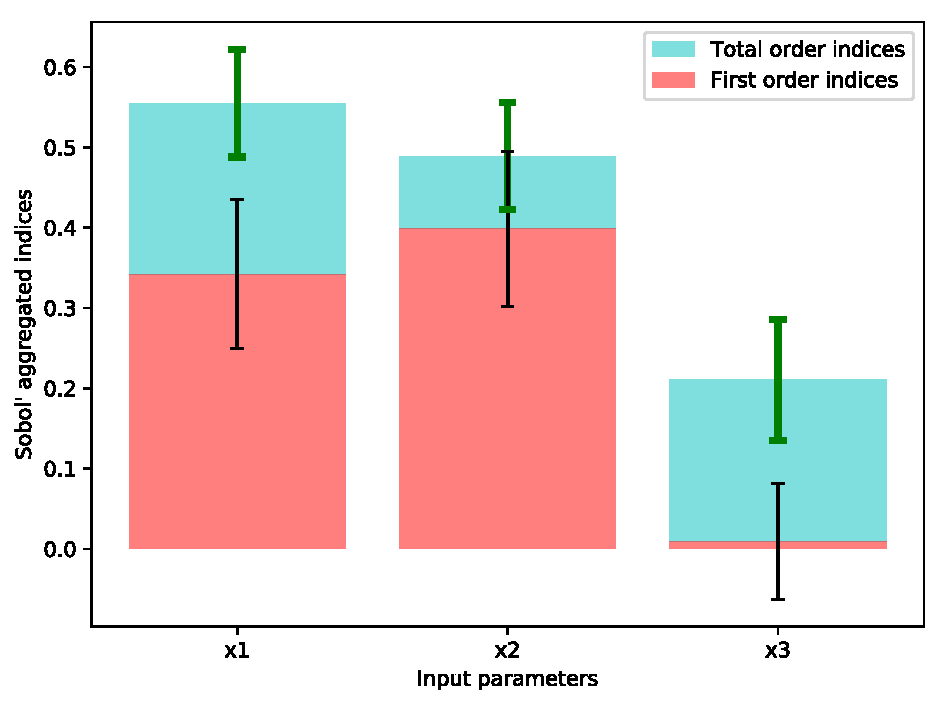
\includegraphics[width=0.6\linewidth,height=\textheight,keepaspectratio]{fig/literature/sobol_aggregated.pdf}}
~
\subfloat[Convergence of the \emph{Sobol'} indices]{
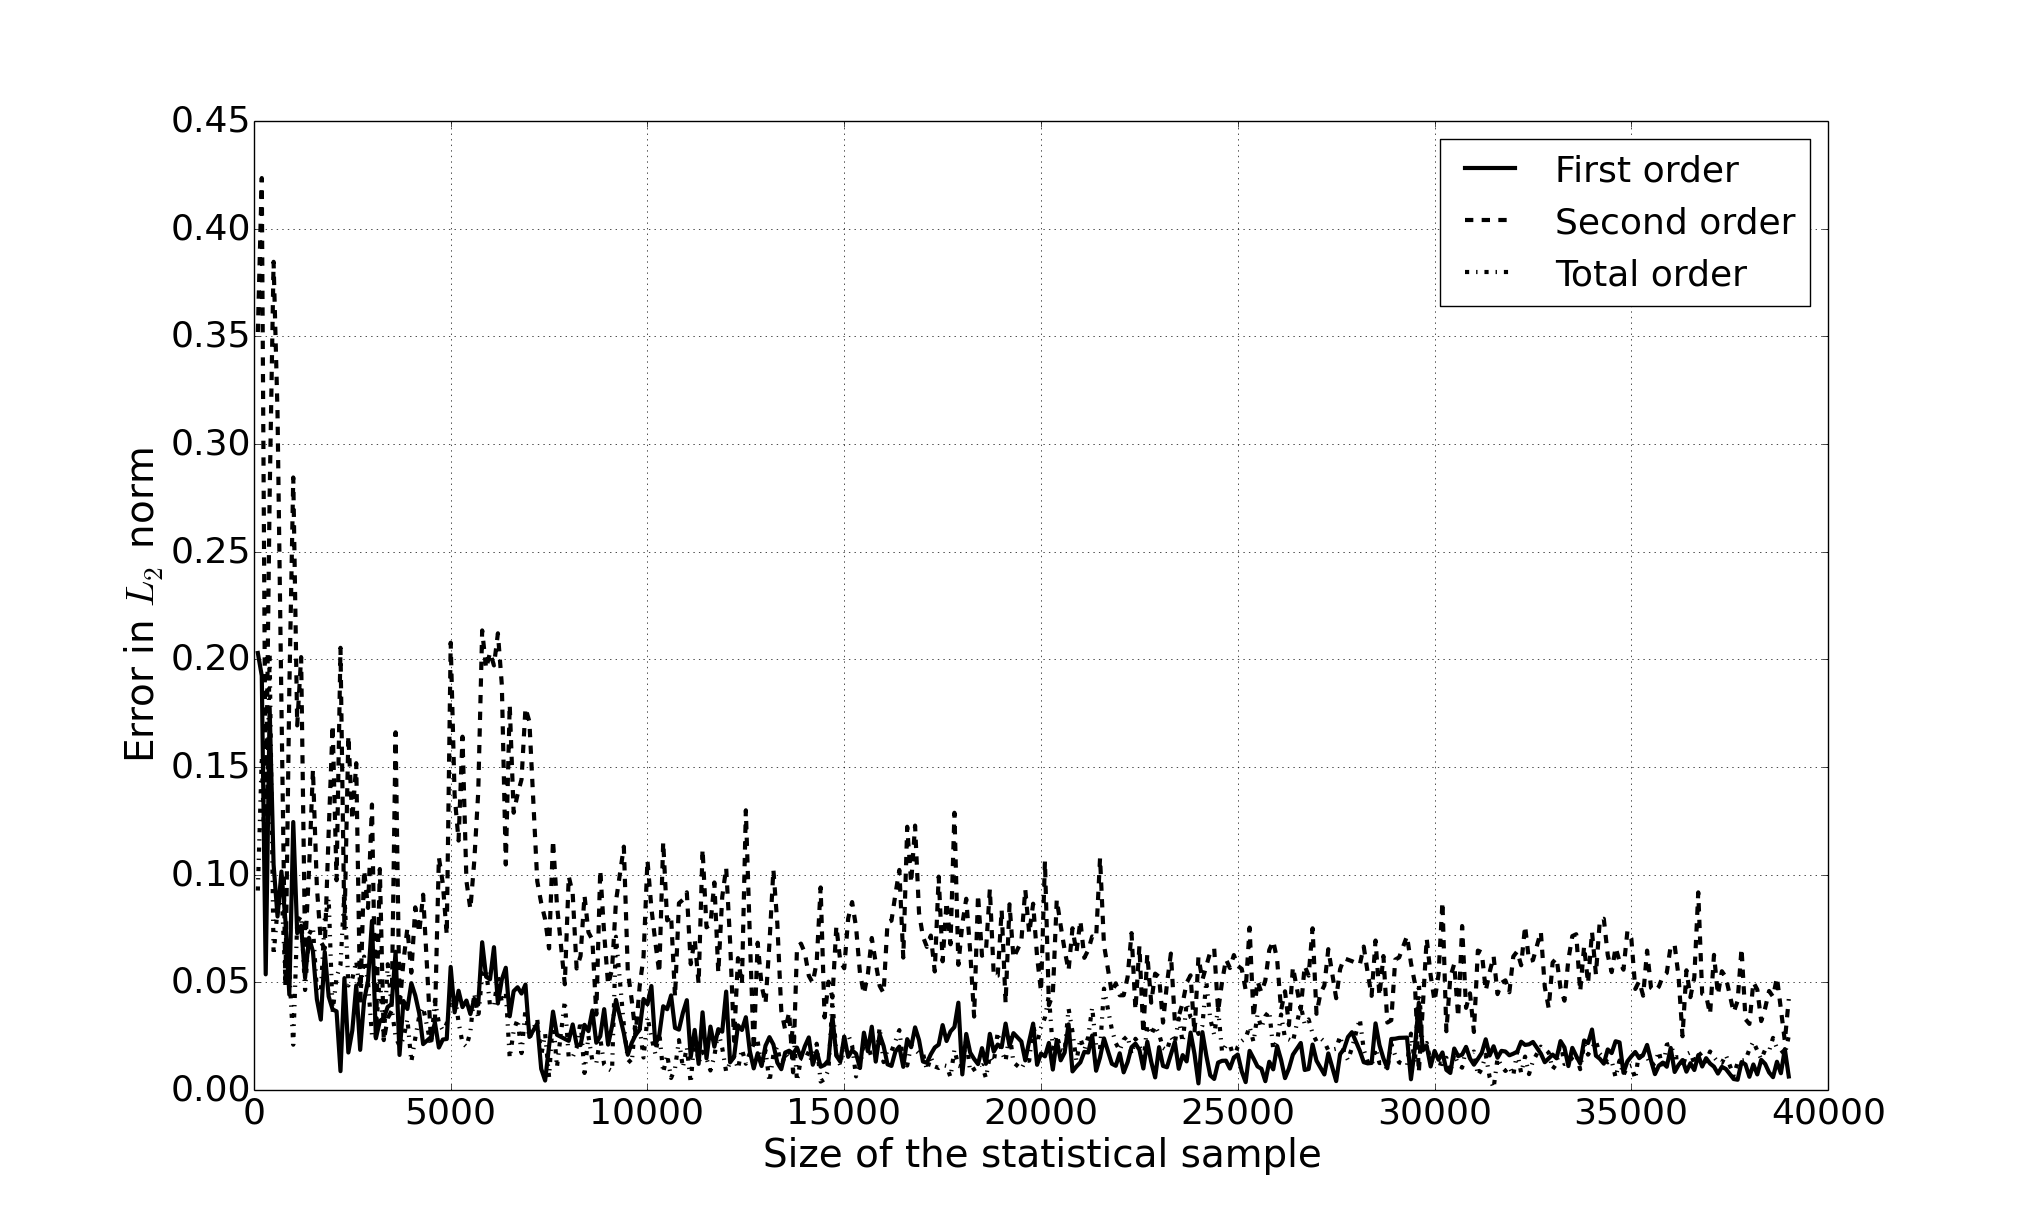
\includegraphics[width=0.6\linewidth,height=\textheight,keepaspectratio]{fig/literature/l2_sample.png}}
\caption{First and total \textit{Sobol'} indices with confidence intervals on the Ishigami function.}
\label{fig:sobol}
\end{figure}


\begin{figure}[!ht]
\centering
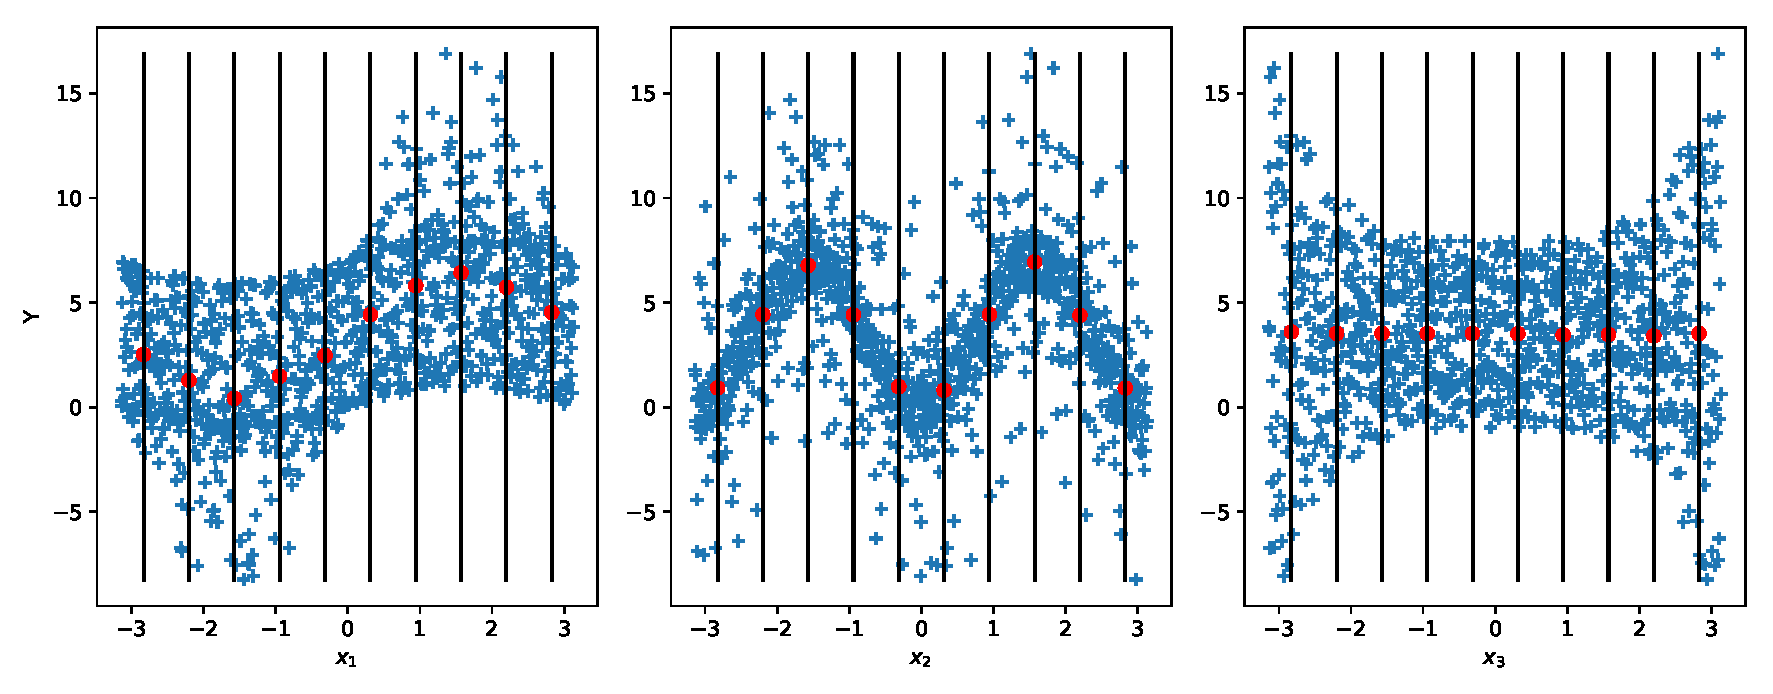
\includegraphics[width=\linewidth,keepaspectratio]{fig/literature/scatter_sobol.pdf}
\caption{Scatter plot per component of the \textit{Ishigami} function. \emph{Blue crosses} represent the outputs, \emph{black lines} the conditioning over a given parameter, \emph{red dots} the mean given a conditioning.}
\label{fig:scatter_sobol}
\end{figure}

Classical empirical formulations of \emph{Sobol'} indices require the use of 3 (resp. 4) matrices to compute first and total (resp. and second order indices)~\cite{Saltelli2010}. The computation requires two independent samplings $A$, $B$ of size $N$ and a matrix $AB$ which is a combination of both matrices (resp. $BA$). $AB_{n}$ corresponds to the matrix $A$ with the column $n$ from the matrix $B$. Hence the number of forward model evaluation is $N_s = N(d + 2)$. In~\citep{baudin2016}, they showed that \textit{Martinez}'s formulation is stable and provides asymptotic confidence intervals---approximated with Fisher's transformation---for first order and total order indices. \textit{Martinez}'s estimators write
\begin{align}
\hat{S_i} = \rho (Y(B), Y(AB_{n})) \quad \hat{S_{T_i}} = 1 - \rho (Y(A), Y(AB_n)),
\end{align}
\noindent where $\rho$ is the linear correlation coefficient.

For a functional output, as for the \textit{LS89} blade case---see~\cref{chap:ls89} and \cref{fig:map_sobol}---, \textit{Sobol'} indices can be computed all along the output vector and retrieve a map or create composite indices. As described by Marrel~\cite{marrel2015}, aggregated indices can also be computed as the mean of the indices weighted by the variance at each point or temporal step
\begin{align}
S_i = \frac{\displaystyle\sum_{l = 1}^{m} \mathbb{V} [\mathbf{Y}^l] S_i^{l}}{\displaystyle\sum_{l = 1}^{m} \mathbb{V} [\mathbf{Y}^l]}.
\end{align}

\begin{figure}[ht]
\centering
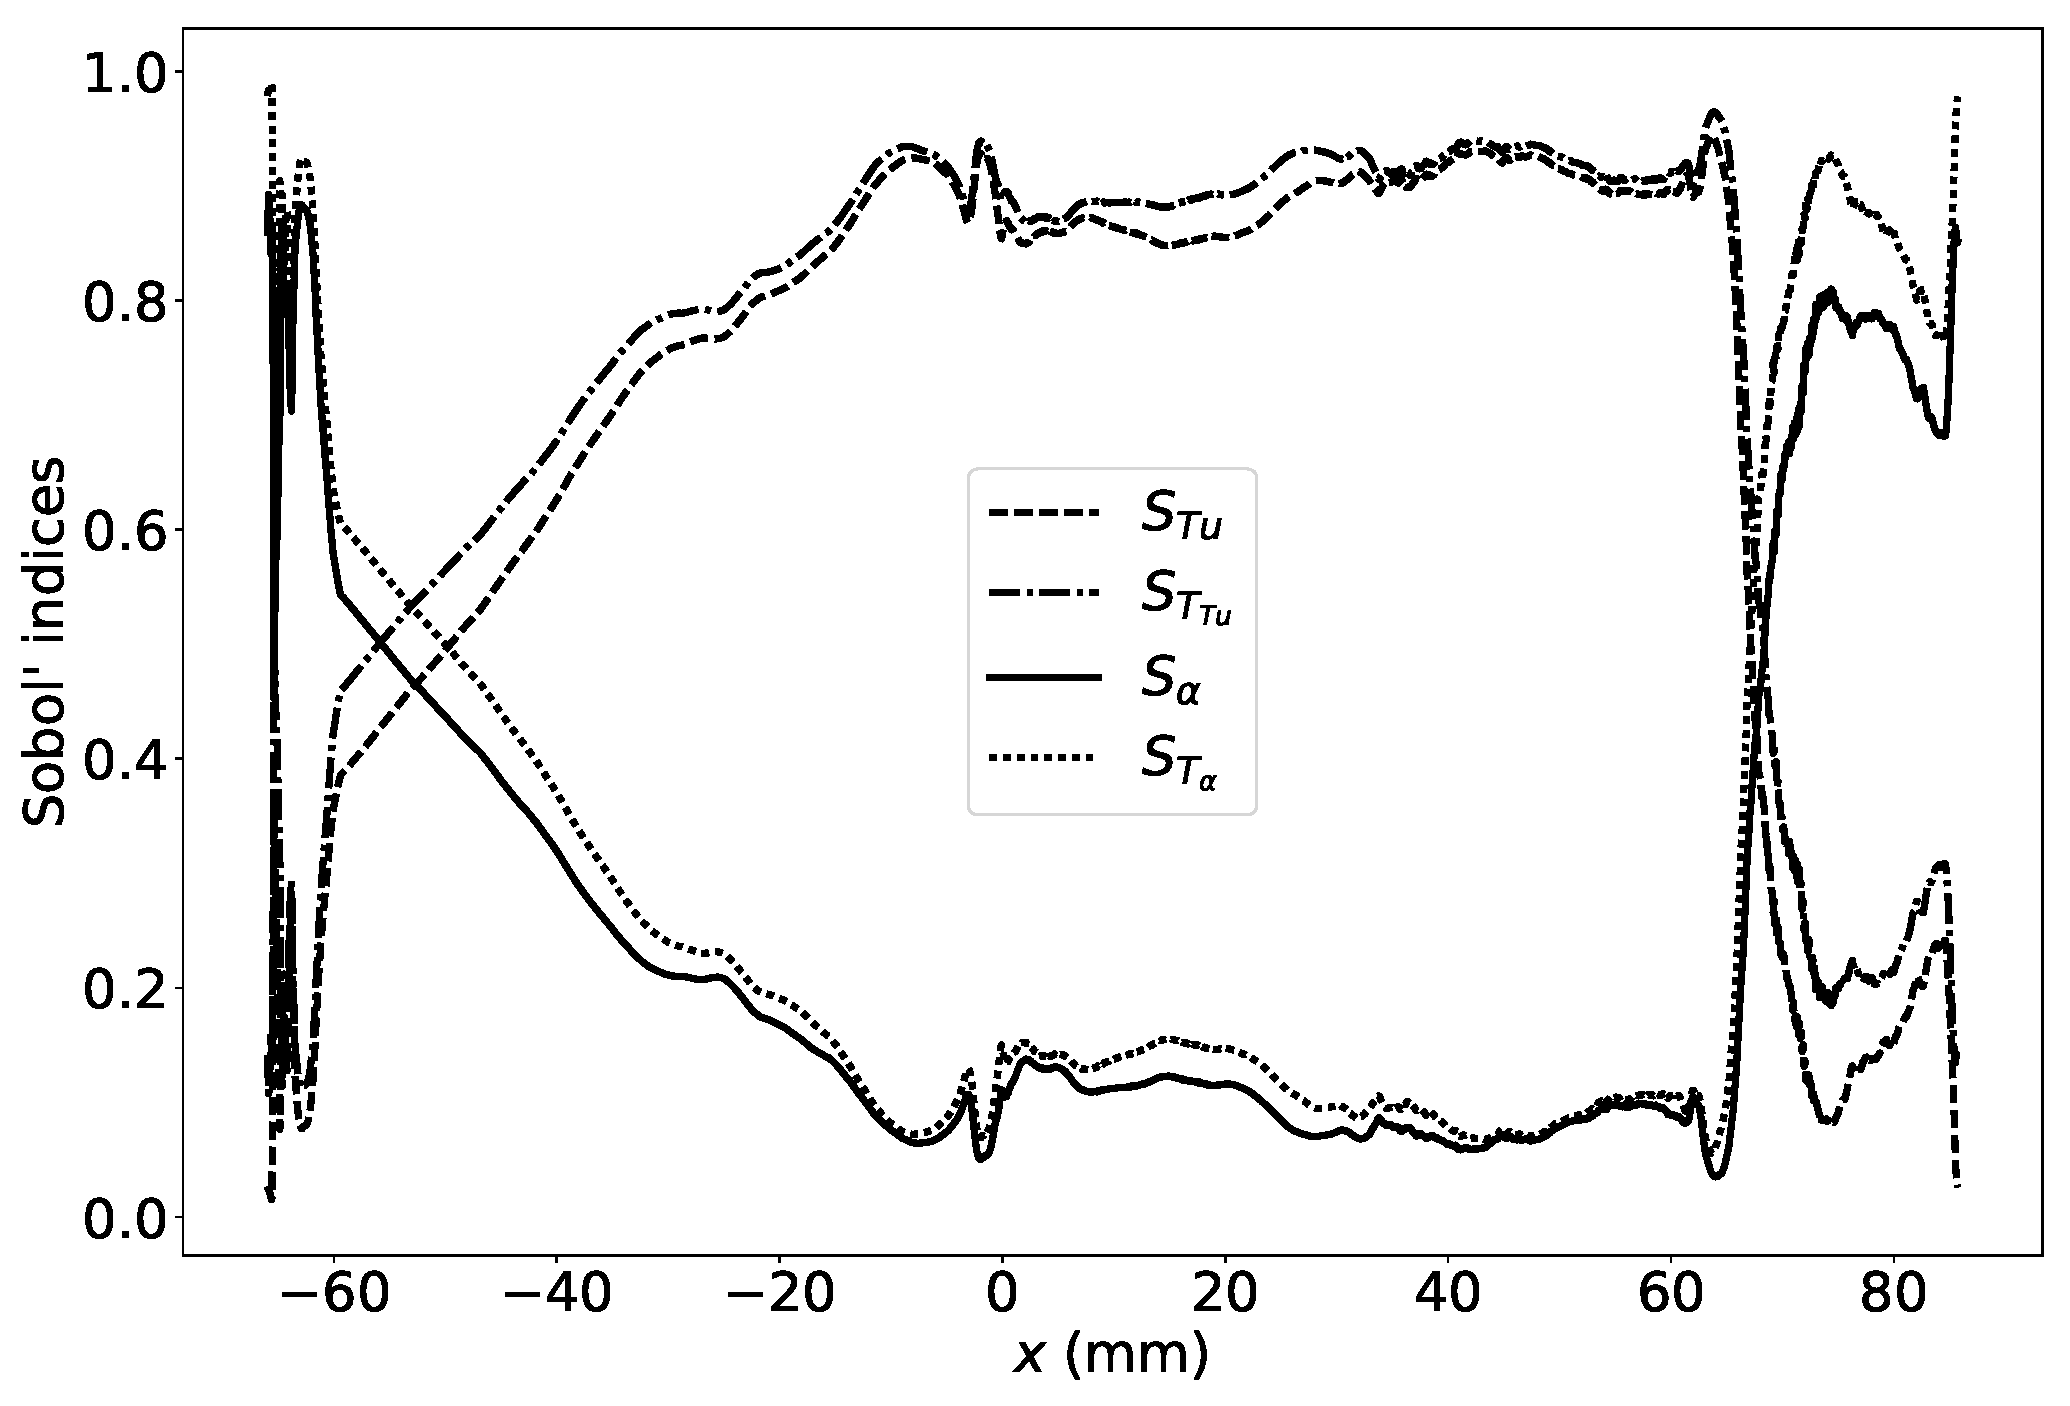
\includegraphics[width=0.8\linewidth,keepaspectratio]{fig/literature/sobol_map.pdf}
\caption{Map of \emph{Sobol'} indices of two input parameters $T_{u}$ and $\alpha$ along the curvilinear abscissa $x$ of the \textit{LS89} blade.}
\label{fig:map_sobol}
\end{figure}

A note regarding the independence of the input parameters. If the nature of the dependence in terms of probability distribution function is known---through copula-based approach for instance~\cite{caniou2012}---, the \emph{Sobol'} formulation can be extended~\cite{Kucherenko2012,Kucherenko2017,Iooss2017}.

\subsubsection{Moment-based Sensitivity Analysis}
Variance-based SA are standard methods (although elementary effects or classical regression are still commonly used among practitioners~\cite{ferretti2016}) but they do not come without flaws~\cite{borgonovo2016}:

\begin{itemize}
\item \emph{Only the second order moment is taken into account,}\\
It means that if the QoI's PDF is highly skewed, multimodal or with heteroscedastic data, this information will be lost. Hence, the variance is only a good measure if the distribution is close to normal.
\item \emph{The parameters need to be independent,}\\
This assumption can be mitigated by using some correlation matrices but the procedure is not really trivial.
\item \emph{Null first order indices does not imply that the parameter is independent with the QoI,}\\
Computation of high-order terms and total effect require a lot of samples to converge. It may be impractical to compute these quantities.
\end{itemize}

Moment-based methods are based on the whole PDF to mitigate these issues~\cite{borgonovo2007}. Based on the unconditional PDF, a conditional PDF per parameter is computed. The more the conditional PDF deviates from the unconditional PDF, the more the parameter has an impact on the quantity of interest. The same procedure can be done using the Empirical Cumulative Density Function (ECDF), respectively with the unconditional ECDF. \Cref{fig:scatter_moments} visually shows this procedure. Bins of samples (\emph{red circles}) are used to compute a conditional PDF of the output. This PDF is compared to the unconditional PDF.

\begin{figure}[!ht]
\centering
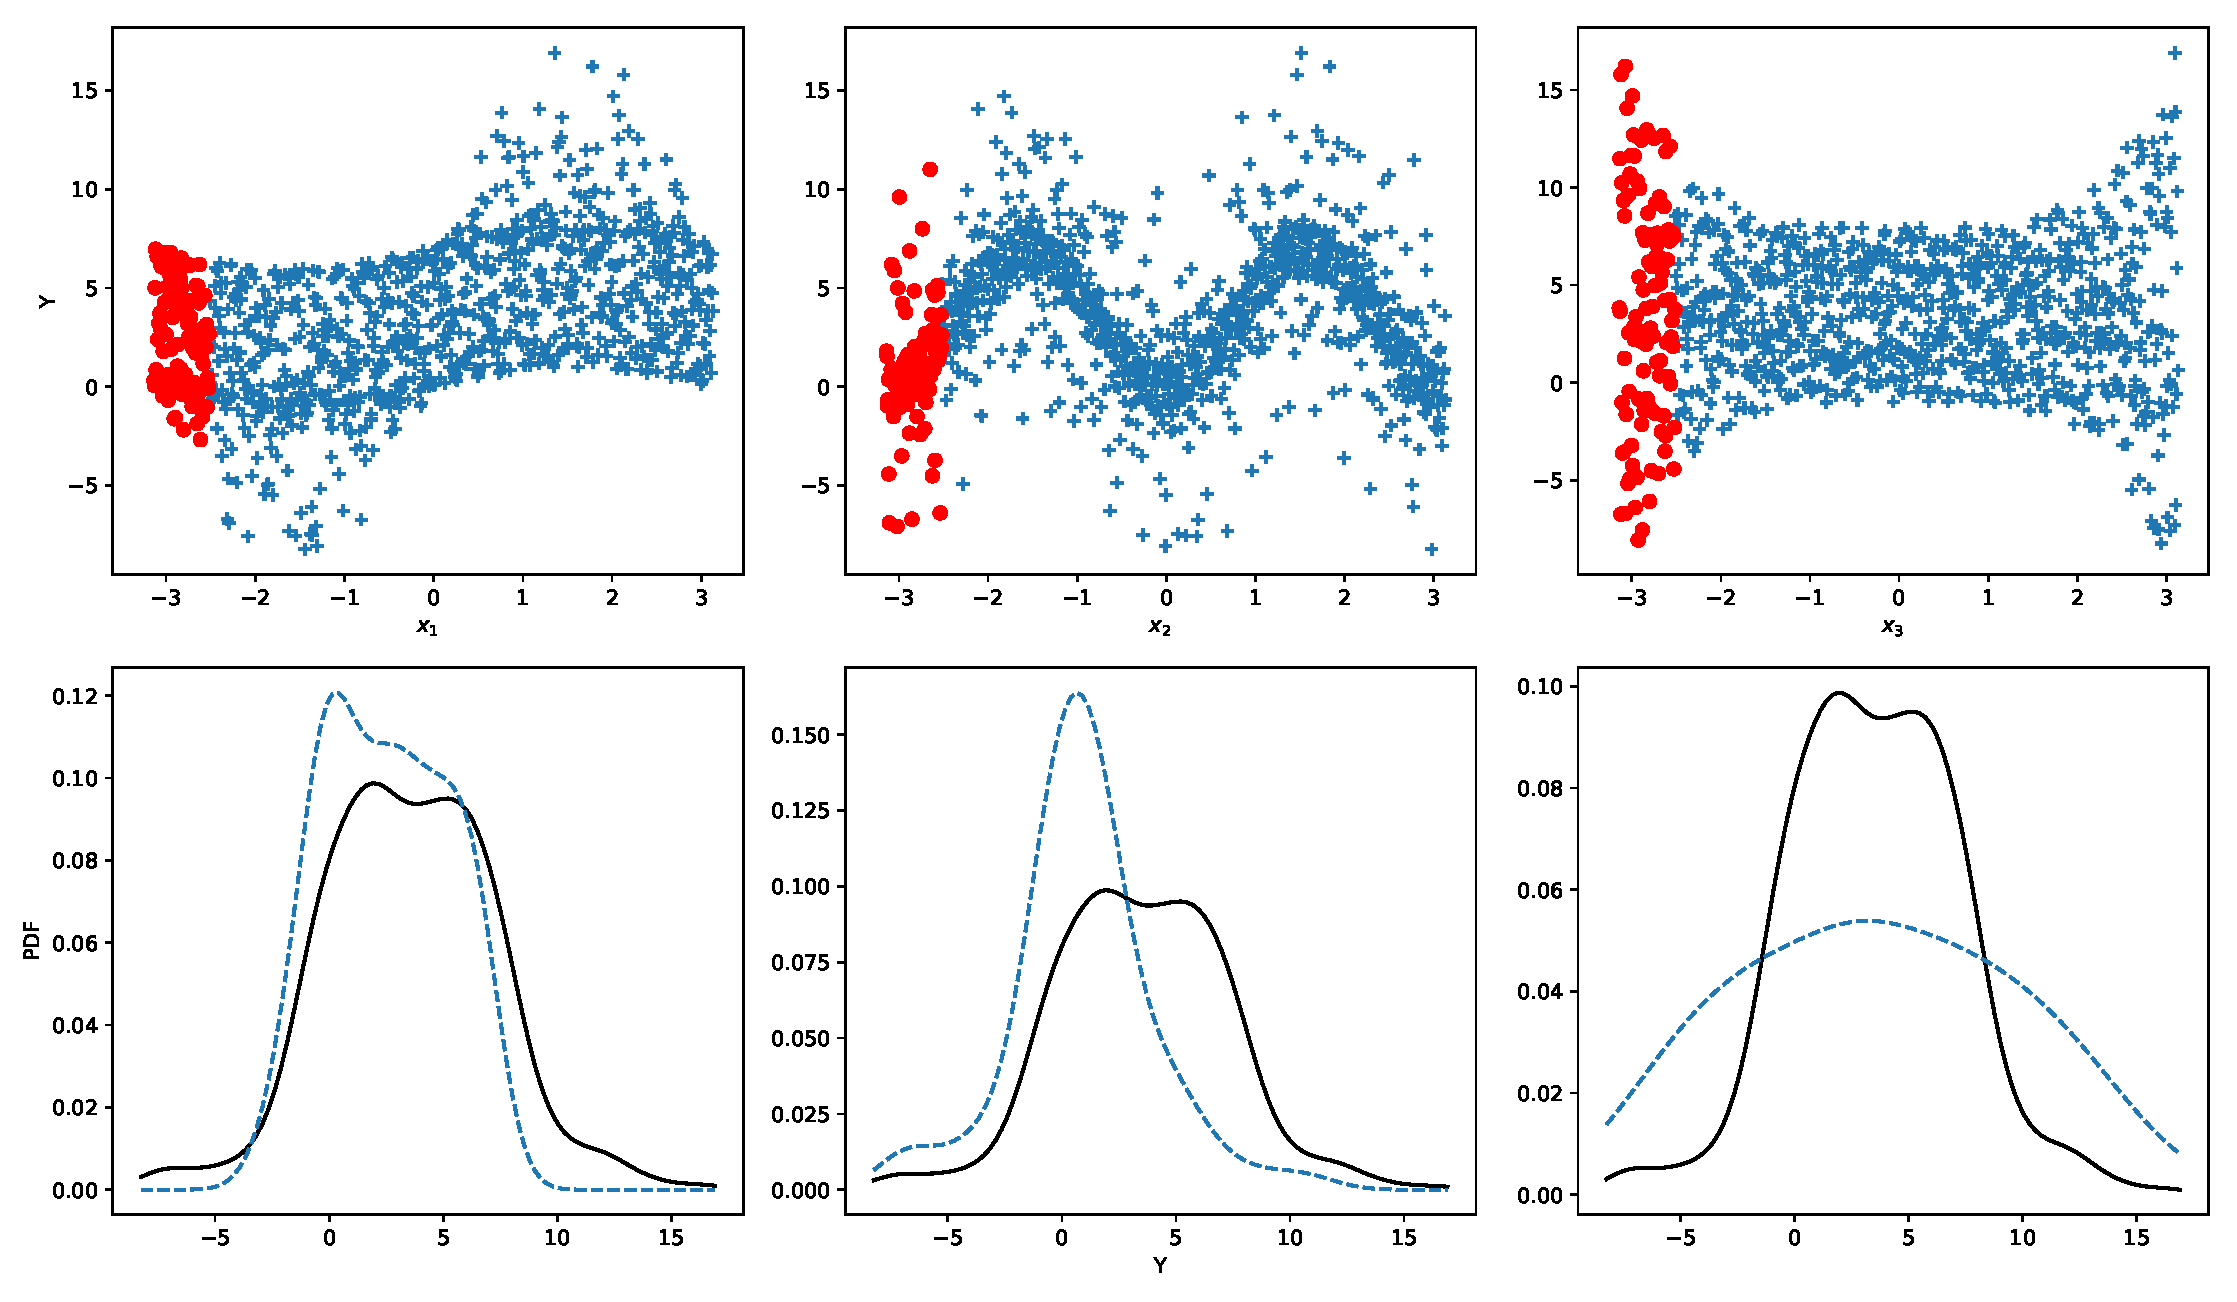
\includegraphics[width=\linewidth,keepaspectratio]{fig/literature/scatter_moments.pdf}
\caption{Scatter plot per component of the \textit{Ishigami} function. \emph{Black line} represents the unconditional PDF and \emph{red dots} the samples used to compute the conditioned PDF shown in \emph{dashed line}.}
\label{fig:scatter_moments}
\end{figure}

\Cref{fig:moment_sa} shows the computation of both conditional and unconditional PDF (resp. ECDF). Based on these moment estimations, distance criteria can be computed such as: $L_1$, \emph{Kolmogorov-Smirnov} or the \emph{Kuiper} distances. The method does not require any particular sampling nor do not require the parameters to be independent. The limitations comes from the ability to correctly estimate the density and from the interpretation of some metrics as they might not be adimensionalized as \emph{Sobol'} indices.

\begin{figure}[!ht]
\centering
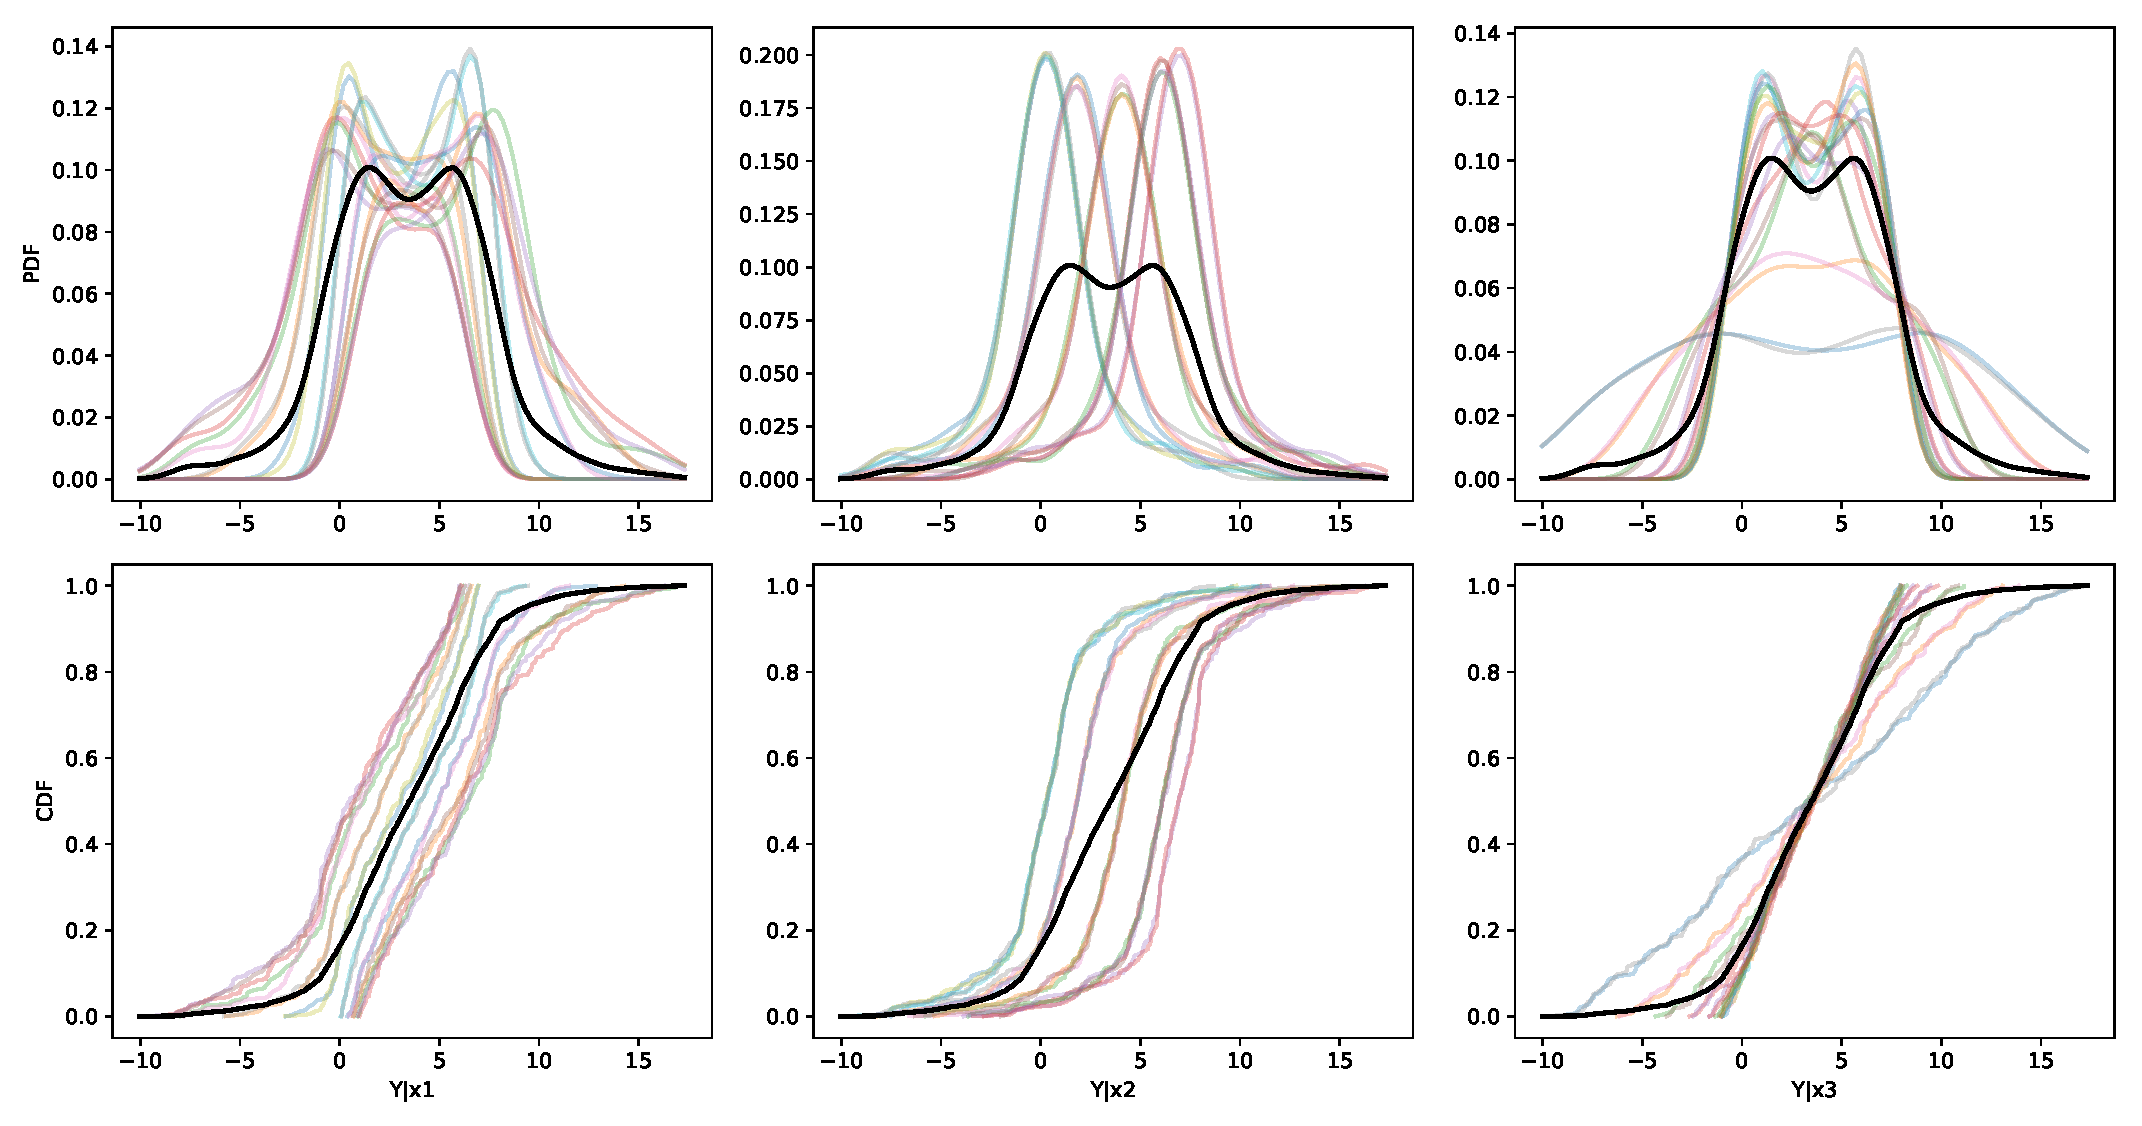
\includegraphics[width=\linewidth,keepaspectratio]{fig/literature/moment_independent-ishigami.pdf}
\caption{Moment independent SA on the \emph{Ishigami} function.}
\label{fig:moment_sa}
\end{figure}

Another visual approach is found with the Cumulative Sums Of NOrmalized Reordered Output method (CUSUNORO)~\cite{Plischke2012}. The output is normalized and ordered in function of a given parameter. Then, its cumulative sum vector is computed. In other words, this corresponds to the conditional ECDF after normalization. Here as well, the more the curve is far from the unconditional ECDF (a flat line after normalization), the more the output is sensitive to the parameter---see~\cref{fig:cusunoro}.

\begin{figure}[!ht]
\centering
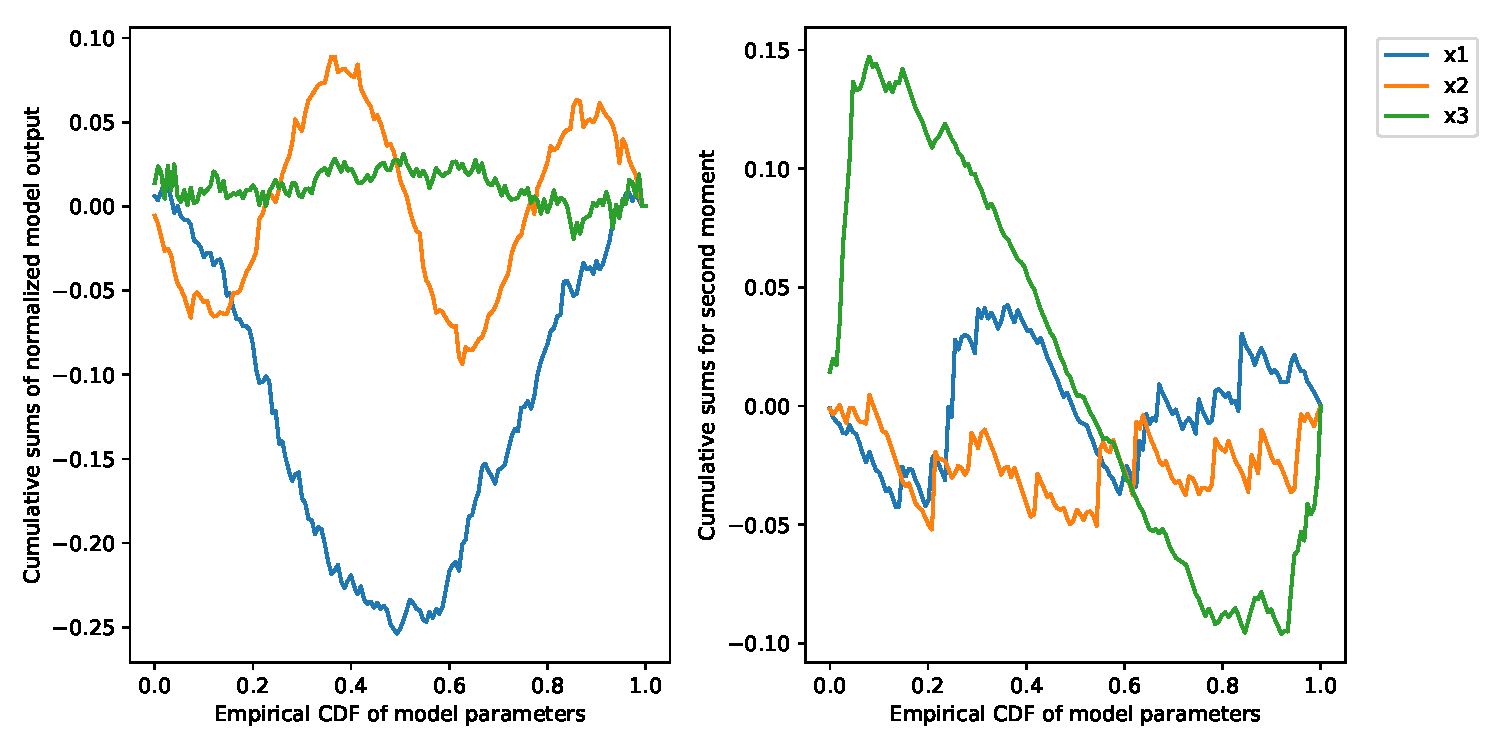
\includegraphics[width=\linewidth,keepaspectratio]{fig/literature/cusunoro-ishigami.pdf}
\caption{CUSUNORO on the \emph{Ishigami} function.}
\label{fig:cusunoro}
\end{figure}

\newpage

\section{Surrogate Models}\label{sec:surrogate}

\lettrine{C}{lassical} UQ methods, based on the Monte-Carlo approach, require a large number of experiments~\citep{iooss2010,iooss2016,lamboni2011,lemaitreknio2010,Saltelli2007,storlie2009}, which quickly go beyond the limits of available resources (CPU cost, budget). In the following, numerical simulations are considered and especially CFD simulations. These limits are especially true when it comes to large-dimensional problems, both with respect to the domain discretization and to the number of uncertain input parameters. Depending on the fidelity sought, one high fidelity simulation can cost millions hours of computing time. The cost of the UQ study can, however, be significantly reduced when the CFD code is replaced by a surrogate model which is formulated in a parameter space and which is fast to evaluate for any set of uncertain variables~\cite{martin2005}.

Before going further, let us clarify the nature of the forward model. The ensemble $\mathcal{Y}$ constitute a set of observed QoI. Each element can either be a scalar or a vectorial---or functional---QoI. When considering scalar QoI, a global physical parameter such as the mean temperature for instance, a single surrogate model mapping $Y^{(i)} := \mathcal{M}(\mathbf{x}^{(i)})$ can be constructed. In case of a multidimensional output, one can consider independent surrogate for each element but the computational cost can rapidly become intractable. Moreover, the elements of the vectorial QoI can be correlated. A classical solution is found through the use of a Proper Orthogonal Decomposition (POD)~\cite{AnindyaChatterjee2000}. By performing a POD on the QoI, each mode being orthogonal, they can be treated as independent and then a surrogate model can be built on a reduced space. In~\cite{braconnier2011,margheri2016}, this method was used to reduce the computational cost and conserve the spatial/temporal correlation of the QoI.

Formulating the surrogate model relies on a limited number of forward model integrations referred to as the DoE. Several surrogate models are found in the literature, among whom generalized linear models, polynomial models, splines, Polynomial Chaos (PC) expansions, artificial neural networks or Gaussian Process (GP) models. In this work, two types of surrogate models are used to approximate the behaviour of forward models. PC expansion on the one hand, GP regression on the other hand. 

PC approach has received much attention lately~\citep{dubreuil2014,sudret2008,xiu2010,xiu2002,Ciriello2013}. The PC surrogate model is formulated as a polynomial expansion, in which the basis is defined according to the distribution of the uncertain inputs $\mathbf{x}$ and the coefficients relate to the statistics of the output $\mathbf{Y}$. The coefficients are computed so as to fit the training set $(\mathbf{X}, \mathcal{Y})$, either using regression or spectral projection methods. The merits of PC surrogates were demonstrated in various fields, e.g.~structural mechanics~\citep{dubreuil2014,berveiller2005}, CFD~\citep{hosder2006,lucor2007,saad2007phd}, hydrology~\citep{deman2015}, hydraulics~\citep{ge2008,elmocaydphd}, wildfires~\citep{rochoux2014}. A complementary approach between PC and EnKF was presented in~\citet{lixiu2009} and tested in the framework of wildfire behaviour forecasting in~\citet{rochoux2014}. 

GP that is strongly related to Kriging in geostatistics also is of increasing interest~\citep{rasmussen2006,legratiet2017,lockwood2012,marrel2015}. The GP formalism treats the forward model response as a realization of a Gaussian stochastic process indexed by $\mathbf{x}$ and fully characterized with mean and covariance functions conditioned by the training set $(\mathbf{X}, \mathcal{Y})$. The GP surrogate is built first, by defining a covariance kernel function between output values and a trend function and then, by estimating the hyperparameters (e.g.~variance, characteristic length scale) that provide a good fit to the training set. GP surrogates were introduced in the context of SA for estimating \emph{Sobol'} indices~\citep{oakley2004,marrel2009,legratiet2014}. In an industrial context---which is the case here---, some benefits of this method are:\textit{(i)} it does not require any prior knowledge of the probability distribution of the uncertainties on the input parameters ; \textit{(ii)} it does not need a specific sampling of the parameter space which could lead to \textit{curse-of-dimensionality} or mis-evaluation of the space ; and \textit{(iii)} it provides an estimation of the predictive error.

PC and GP surrogate models have recently been compared for UQ and SA studies~\citep{legratiet2017,owen2015,Schoebi2015}. \citet{owen2015} evaluated the performance of each type of surrogate in terms of output mean, variance and PDF estimation. \citet{legratiet2017} compared \emph{Sobol'} indices with applications in structural mechanics; for a given size of the training set, PC and GP surrogate models were found to feature a similar predictive quality---with respect to the predictive coefficient $Q_2$, also called Nash-Sutcliffe model efficiency coefficient, which is equivalent to the coefficient of determination $R^2$ for residuals's prediction~\citep{krause2005} (see~\cref{sec:validation}). \citet{legratiet2017} also emphasized that the ranking between PC and GP approaches remains problem-dependent.

Considering the general case of a functional QoI, the common idea of PC and GP approaches is to design for each element (with or without considering a POD) $a \in \{a_1, \cdots, a_M\}$ a surrogate with a weighted finite sum of basis functions:
\begin{align}
\widehat{Y}_a\left(\mathbf{x}\right) = \displaystyle\sum_{i = 0}^{r}\,\gamma_{a,i}\,\Psi_{i}\left(\mathbf{x}\right),
\label{eq:SurrogateForm}
\end{align}
where the coefficients $\gamma_{a,i}$ and the basis functions $\Psi_i$ are calibrated by the training set $\mathbf{X}^{N_s}$. The main difference between PC (Sect.~\ref{sec:PC}) and GP (Sect.~\ref{sec:GP}) approaches stands in the nature of these models: GP interpolates the training points and captures local variations, while PC is a regression method focusing on the global behaviour of the model. Basis functions and calibration methods also differ between these two approaches.

\Cref{sec:POD} present the POD while \cref{sec:PC} and \cref{sec:GP} respectively defines the PC and the GP surrogate methods. An overview of methods combining several level of fidelity is done in~\cref{sec:evofusion}. Finally, in~\cref{sec:validation} we present quality metrics associated with surrogate models.

\subsection{Snapshot Method}\label{sec:POD}

% TODO Différence avec Kahrunen Loeve - SVD : maillage irrégulier

The key idea of the snapshot method~\citep{sirovich1987} is to achieve a POD of the centred snapshot matrix $\mathcal{Y} \in \mathbb{M}_{M,N}(\mathbb{R})$, which gathers the discretized QoI for the $N_{s}$ snapshots, from which the sample mean is subtracted. For simplicity purpose, the QoI anomaly element $a$ is denoted $y$ in the following. Thus, $\mathcal{Y} = \left(y_{a_i}^{(j)}\right)_{1\leq i \leq M \atop 1\leq j \leq N_{s}}$. The snapshots correspond to the column vectors; the $k$th snapshot of size $M$ is denoted by $\mathbf{y}^{(k)}$.

Based on many observations of a random vector, the POD gives the orthogonal directions of largest variances (or modes) in the probabilistic vector space in order to reduce the vector space dimension~\citep{chatterjee2000}. Note that for simplicity purpose, the adjective {\it centred} is dropped in the following when referring to the centred snapshot matrix $\mathcal{Y}$.

The POD of the snapshot covariance matrix $\mathbf{C} = N_{s}^{-1}\,\mathcal{Y}^{\mathrm{T}}\,\mathcal{Y}\in \mathbb{M}_{N_{s}}(\mathbb{R})$ is equivalent to the Singular Value Decomposition (SVD) of the snapshot matrix $\mathcal{Y}$:
\begin{align}
\mathcal{Y} = \mathbf{U}\,\mathbf{\Lambda}\,\mathbf{V}^{\mathrm{T}} = \displaystyle\sum_{k = 1}^{r_{p}}\,\lambda_k\,\mathbf{u}_k\,\mathbf{v}_k^{\mathrm{T}},
\end{align} 
where $\mathbf{U} \in \mathbb{M}_M(\mathbb{R})$ is an orthogonal matrix diagonalizing $\mathcal{Y}\mathcal{Y}^{\mathrm{T}}$ ($\mathbf{u}_k$, the $k$th column of $\mathbf{U}$, is a left singular vector of $\mathcal{Y}$), where $\mathcal{V} \in \mathbb{M}_{N_{s}}(\mathbb{R})$ is an orthogonal matrix diagonalizing $\mathcal{Y}^{\mathrm{T}}\mathbf{Y}$ ($\mathbf{v}_k$, the $k$th column of $\mathbf{V}$, is a right singular vector of $\mathcal{Y}$), and where $\mathbf{\Lambda} \in \mathbb{M}_{M,N_{s}}(\mathbb{R})$ is a rectangular diagonal matrix including $r_{p}=\min(M,N_{s})$ singular values on its diagonal. The singular values $\lbrace \lambda_k \rbrace_{1 \leq k \leq r_{p}}$ are the square roots of the eigenvalues of $\mathbf{C}$. 
Note that in the following, we do not reduce further the rank of the snapshot matrix $\mathcal{Y}$. 

For a given element $a$, any snapshot $h_a(\mathbf{x}^{(k)})$ can then be retrieved as a linear combination of $r_{p}$ modes $\{\Psi_i\}_{1\leq i \leq r_p}$:
\begin{align}\label{eq:gppod}
y_a(\mathbf{x}^{(k)}) 
= (\mathbf{U}\,\mathbf{\Lambda}\,\mathbf{V}^{\mathrm{T}})_{ak} 
= U_{a:}(\mathbf{\Lambda}\,\mathbf{V}^T)_{:k}=\sum_{i=1}^{r_{p}}\,\gamma_{a,i}\,\Psi_i(\mathbf{x}^{(k)}),
\end{align}
where for any $i\in\{1,\ldots,M\}$, $\gamma_{a,i}:=U_{a,i}$ and $\Psi_i(\mathbf{x}^{(k)}):=(\boldsymbol{\Lambda}\mathbf{V}^T)_{i,k}$. 

\Cref{fig:pod} is a visual explanation of the POD on the El Ni\~no dataset---see~\cref{sec:dataset}. A POD is performed on the dataset composed of $N_s=54$ curves. The first two modes account respectively for 73\% and 15\% of the variance of the data. \Cref{fig:pod}(a) presents a visualization of the same dataset in this 2-dimensional reduced space. Hence, each point of the reduced space is associated to a curve in the original space. \Cref{fig:pod}(c) shows the individual contribution of each modes for a given sample while \cref{fig:pod}(d) is the sum of these contributions (plus the sample mean). Due to the modal truncation, there is a loss of information.

\begin{figure}[!ht]               
\centering
\subfloat[Dataset]{
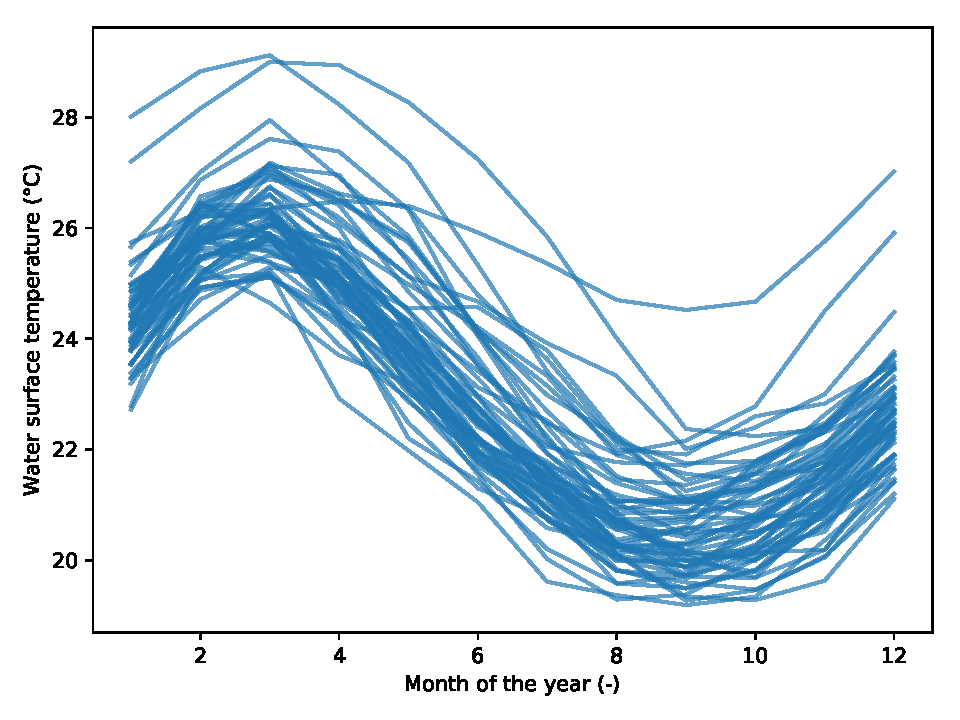
\includegraphics[width=0.48\linewidth,height=\textheight,keepaspectratio]{fig/literature/dataset_elnino.pdf}}
~
\subfloat[Reduced space]{
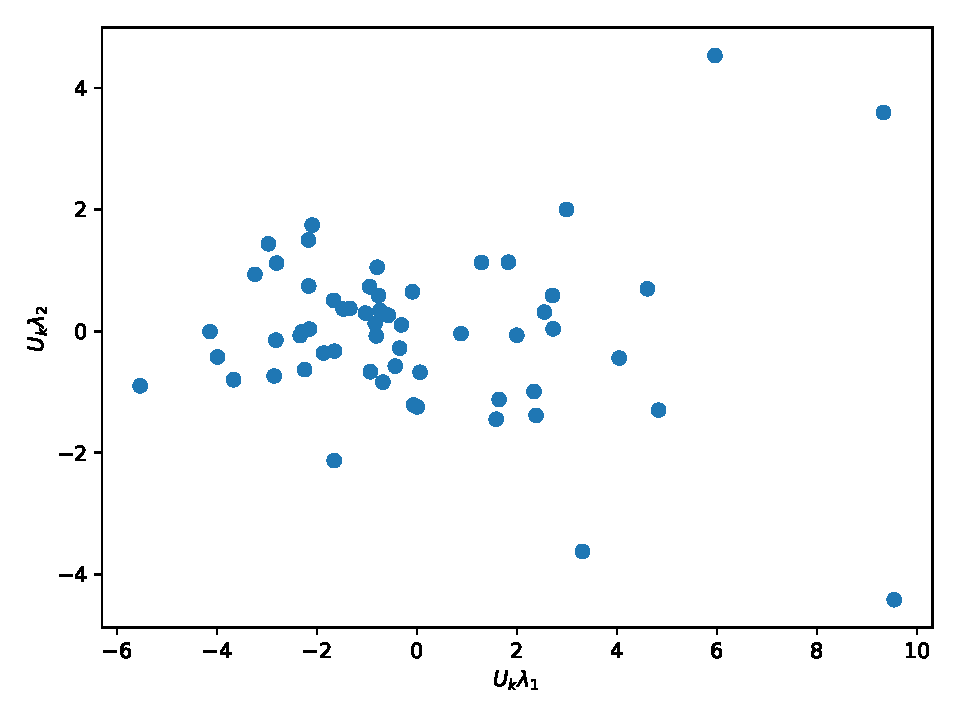
\includegraphics[width=0.48\linewidth,height=\textheight,keepaspectratio]{fig/literature/dataset_elnino-r.pdf}}

\subfloat[Modes]{
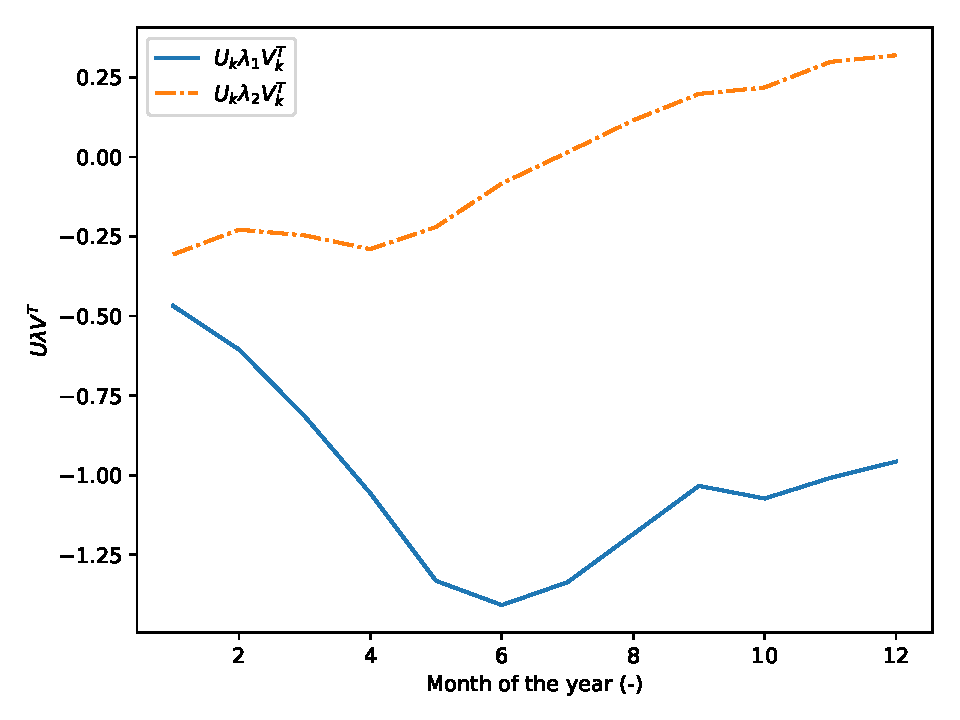
\includegraphics[width=0.48\linewidth,height=\textheight,keepaspectratio]{fig/literature/dataset_elnino-modes.pdf}}
~
\subfloat[Reconstruction]{
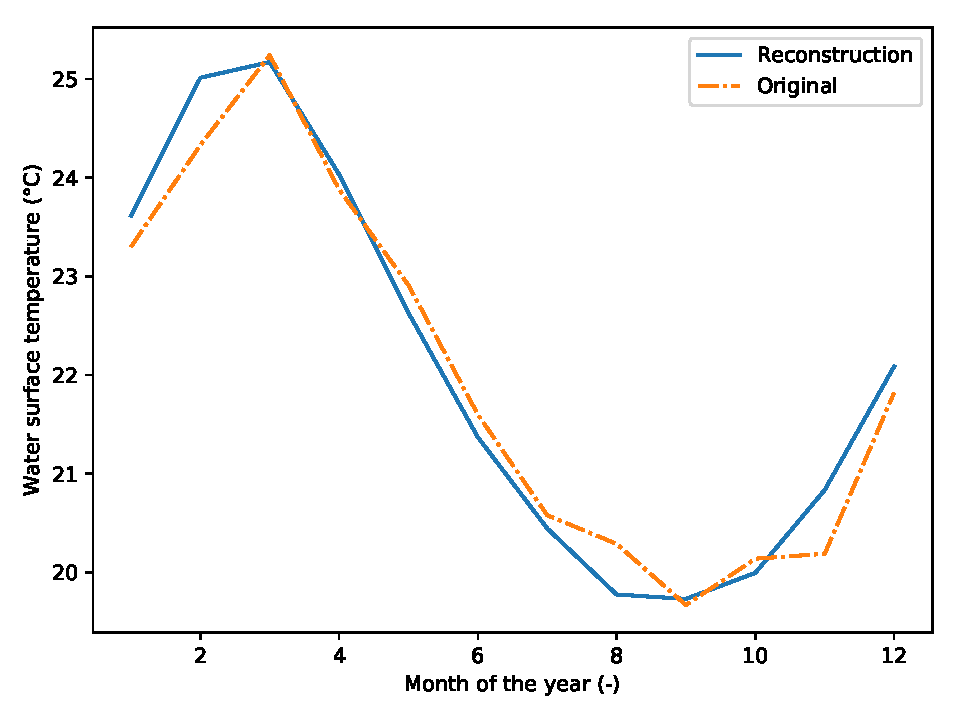
\includegraphics[width=0.48\linewidth,height=\textheight,keepaspectratio]{fig/literature/dataset_elnino-reconst.pdf}}
\caption{POD reconstruction principle applied to the El Ni\~no dataset. \emph{Top figures} present a decomposition of the dataset into a reduced space using two components. \emph{Bottom figures} present the reconstruction of a sample.}
\label{fig:pod}
\end{figure}

\bigskip
%----Polynomial Chaos
\subsection{Polynomial Chaos Surrogate Model}\label{sec:PC}

The algorithm to build the PC surrogate proceeds as follows:
\begin{enumerate}
\item choose the polynomial basis $\lbrace\Psi_{i}\rbrace_{i\geq 0}$ according to the assumed PDF of the inputs $\mathbf{x}$,
\item choose the total polynomial degree $P$ according to the complexity of the physical processes,
\item truncate the expansion to $r_{\text{pc}}$ terms to keep the predominant information given by the forward model using standard truncation strategy ($r_{\text{pc}}$ depends on $d$ and $P$ and is defined further on),
\item apply spectral projection strategy (i.e.~Gaussian quadrature rule) to compute the coefficients $\lbrace\gamma_{a,i}\rbrace_{i\in\mathbb{N}^d\atop|i|\leq P}$ for each element $a$ (can use a POD or not) using $N_{s} = (P+1)^{d}$ snapshots,
\item formulate the surrogate model $\mathcal{M}_{\text{pc}}$ at each element $a$, which can be evaluated for any new pair of parameters $\mathbf{x}^*$.
\end{enumerate}
Note that we use standard truncation and projection strategies presented in~\cite{lemaitreknio2010} and \cite{xiu2010}.

\subsubsection{Polynomial Basis}

Each component of the random vector $\mathbf{x}$ defined in the input physical space is standardized and noted by $\boldsymbol{\zeta}$ in the following way: $\zeta_i=\frac{x_i-\mu_i}{\sigma_i}$ where $\mu_i=N_{s}^{-1}\sum_{k=1}^{N_{s}}x_i^{(k)}$ and $\sigma_i=\sqrt{(N_{s}-1)^{-1}\sum_{k=1}^{N_{s}}\left(x_i^{(k)}-\mu_i\right)^2}$. 

%Assuming that the SWE solution is of finite variance, each component $h_a$ of the water level vector $\mathbf{h}$ can be considered as a random variable for which there exists a polynomial expansion of the form~\eqref{eq:SurrogateForm} that represents how the water level $h_a$ varies according to changes in $Q$ and $K_{s_3}$. 

$y_a$ is projected onto a stochastic space spanned by the orthonormal polynomial functions $\lbrace\Psi_{i}\rbrace_{i\geq 0}$. These functions are orthonormal with respect to the joint density $\rho(\boldsymbol{\zeta})$, i.e.
\begin{align}
\int_{Z}\,\Psi_i(\boldsymbol{\zeta})\,\Psi_j(\boldsymbol{\zeta})\,\rho(\boldsymbol{\zeta})\,\mathrm{d}\boldsymbol{\zeta} = \delta_{ij},
\label{eq:pc_innerproduct}
\end{align}
with $\delta_{ij}$ the Kronecker delta function and $Z \subseteq \mathbb{R}^d$ the space in which $\boldsymbol{\zeta}$ evolves.

In practice, the orthonormal basis is built using the tensor product of 1-D polynomial functions: $\Psi_i=\Psi_{i,1}\ldots\Psi_{i,d}$ where $i$ is the multi-index $(i_1,\ldots,i_d)\in\{0,1,\cdots,P\}^d$. The choice for the basis functions depends on the probability measure of the random variables. According to Askey's scheme, the Hermite polynomials form the optimal basis for random variables following the standard Gaussian distribution, and the Legendre polynomials are the counterpart for the standard uniform distribution~\citep{xiu2002}. 

\subsubsection{Truncation Strategy}

In practice, the sum in Eq.~\eqref{eq:SurrogateForm} is truncated to a finite number of terms $r_{\text{pc}}$. Using a standard truncation strategy $r_{\text{pc}}$ is constrained by the number of random variables $d$ and by the total polynomial degree $P$ as:
\begin{align}
r_{\text{pc}} = \frac{(d + P)!}{d!\,P!},
\label{eq:pc_order}
\end{align}
meaning that all polynomials involving the $d$ random variables of total degree less or equal to $P$ are retained in the PC expansion. The PC-approximated QoI at each element $y_{\text{pc}}(a)$ is formulated as:
\begin{align}
\widehat{y}_{\text{pc},a}(\mathbf{x}) := \mathcal{M}_{\text{pc},a}(\boldsymbol{\zeta}) = \displaystyle\sum_{i\in\mathbb{N}^d\atop|i|\leq P}\,\gamma_{a,i}\,\Psi_i\left(\boldsymbol{\zeta}\right).
\label{eq:SurrogatePC}
\end{align}
Note that for small $d$, advanced truncation strategies that consist in eliminating high-order interaction terms or using sparse structure~\citep{blatman2009phd,migliorati2013} are not necessary.

\subsubsection{Spectral Projection Strategy}

We focus here on non-intrusive approaches to numerically compute the coefficients $\lbrace\gamma_{a,i}\rbrace_{i\in\mathbb{N}^d\atop |i|<P}$  in Eq.~\eqref{eq:SurrogatePC} using $N_{s}$ snapshots from $\mathbf{X}^{N_s}$. The spectral projection relies on the orthonormality property of the polynomial basis. The $i$th coefficient $\gamma_{a,i}$ is computed using Gaussian quadrature as:
\begin{align}
\gamma_{a,i} = <y_a,\Psi_i> \,\cong\,\displaystyle\sum_{k = 1}^{N_{s}}\,y_a^{(k)}\,\Psi_i(\boldsymbol{\zeta}^{(k)})\,w^{(k)},
\label{eq:pc_quadrature}
\end{align}
where $\mathbf{y}^{(k)} = \mathcal{M}(\mathbf{x}^{(k)})$ is the snapshot corresponding to the $k$th quadrature root $\mathbf{x}^{(k)}$ of $\Psi_i$ (in the physical space), and where $w^{k}$ is the weight associated with $\mathbf{x}^{(k)}$. $(P+1)$ is the number of quadrature roots required in each uncertain direction to ensure an accurate calculation of the integral $<y_a,\Psi_i>$. Hence, $N_{s} = (P+1)^2$ at least for quadrature strategies.

More advanced technique have been developed in order to reduce the number of sample required using sparse approach~\cite{blatman2009phd,LeMaitre2010,migliorati2013,Shao2017}. Hence, only the most important terms of the expansion are kept in order to lower the sample budget.

% An extended review of the different approaches is out of the scope of this work.

%----Gaussian process
\subsection{Gaussian Process Surrogate Model}\label{sec:GP}

The algorithm to build a Gaussian Process surrogate proceeds as follows:
\begin{enumerate}
\item choose the size of the training set $N_{s}$,
\item draw $N_{s}$ samples (or snapshots) in the input random space $\mathbf{x}$,
%\item formulate the centred snapshot matrix $\mathcal{Y}$ from the $N_{s}$ snapshots,
%\item achieve a POD on $\mathbf{Y}$ using the snapshot method to derive the basis vectors $\lbrace\Psi_{i}\rbrace$ and the corresponding coefficients $\lbrace\gamma_{a,i}\rbrace$ (any snapshot can be expressed as a linear combination of the basis vectors and coefficients),
%\item replace each basis vector $\lbrace\Psi_i\rbrace$ associated to the $N_{s}$ snapshots by a basis function via Gaussian Process regression for any $\mathbf{x}^*$, 
\item formulate the surrogate model $\mathcal{M}_{\text{gp}}$ for the QoI at each element $a$ (can use a POD or not), which can be evaluated for any $\mathbf{x}^*$.
\end{enumerate}

\subsubsection{Regression Procedure}\label{sec:regression}

%In this case, the random variable being the POD coefficients computed for each random input vector $\mathbf{x}$ of $N_s$: $f(\mathbf{x}) = (\mathbf{\Sigma}_{k} \mathbf{V}^T_{k})_{\mathbf{x}}$. A new prediction consists in a new column of $\mathbf{\Sigma}_{k} \mathbf{V}^T_{k}$.

A Gaussian Process (GP) is a collection of random variables which have a joint Gaussian distribution~\cite{rasmussen2006}. GP is equivalent to \textit{Kriging}~\cite{krige1989}. A \textit{Gaussian Process} is described by its mean $\mu(\mathbf{x})$ and covariance $k(\mathbf{x},\mathbf{x}')$---where $\mathbf{x}, \mathbf{x}'$ are different sets of inputs

\begin{align}
Y_a(\mathbf{x})&\sim \mathcal{GP}(\mu(\mathbf{x}), k(\mathbf{x},\mathbf{x}')), \;\text{with} \\
m(\mathbf{x}) &= \mathbb{E}\left[ Y_a(\mathbf{x})  \right], \nonumber \\
k(\mathbf{x},\mathbf{x}') &= \mathbb{E}\left[ (Y_a(\mathbf{x}) -\mu(\mathbf{x}))(Y_a(\mathbf{x}')-\mu(\mathbf{x}')) \right] \nonumber.
\end{align}

Here the covariance function $k$ (or kernel) is chosen as a squared exponential
\begin{align} 
K = k(\mathbf{x}, \mathbf{x}') = \sqrt{\pi} \; \sigma_\mathbf{x}^2 \exp\left(-\frac{\|\mathbf{x} - \mathbf{x}'\|^2}{2\,\ell_i^2}\right), 
\end{align}
where $l$ is a length scale that describes the distance and strength of influence from one sample to another and $\sigma_\mathbf{x}$ is the variance of the output signal. Squared exponential kernel leads to satisfying results but other kernel functions could have been considered, such as a decreasing exponential one or a \emph{Matérn} one -- with their associated hyper-parameters. The choice of the kernel is still an open problem and can be mitigated using the available information on the problem. The square exponential kernel leads to very smooth, thus stable results. Furthermore, it implies that the model is exact at sample points; it does not introduce any other strong assumptions, hence its wide usage among practitioners.

Then the GP model consists of a regression providing an interpolation $\mathcal{M}_{\text{gp}}$ for a new set of input parameters $\mathbf{x^{*}}$:
\begin{align}
\mathcal{M}_{\text{gp}_{a}}(\mathbf{x}^*)&=\bar{Y_{a}}(\mathbf{x}^*) =  \sum_{i = 1}^{N_s}\alpha_i k (\mathbf{x}^i, \mathbf{x}^*), \;\text{with} \\
\mathbf{\alpha} &= (K + \sigma_n^2 I)^{-1}\mathcal{Y}_a, \nonumber
\end{align}
where $\bar{Y_a}$ is the mean realization, $\mathbf{x}^i$ the \textit{i-th} set of parameters, $\mathcal{Y}_{a}$ the snapshot matrix considering element $a$ and $\sigma_n$ is the nugget effect that prevent ill-conditioning issues for the matrix $K$. Indeed, it is the mean realization of the conditioned process considering an artificial noisy observation which gives the prediction. The learning phase of the GP consists in selecting $l$, $\sigma_n$ and $\sigma_\mathbf{x}$ so that $Y_a$ passes through or close to the dataset points. These hyperparameters are optimized by maximizing the log likelihood applied to the data set $\mathcal{Y}_a$ using a basin hopping technique~\citep{wales1997}. A key advantage of this predictor is that it provides an inference about its prediction variance
\begin{align}
\mathbb{V}[Y_{a}(\mathbf{x}^*)] = k(\mathbf{x}^*, \mathbf{x}^*)-\mathbf{k}(\mathbf{x}^*)^T(K + \sigma_n^2 I)^{-1}\mathbf{k}(\mathbf{x}^*).
\end{align}
The regression methodology is shown in~\cref{fig:gp_prior-post}. On \cref{fig:gp_prior-post}(a), the GP is sampled on the input parameter space. In this case, a GP with zero mean and unit variance is used. It means that for each $x^i$, the QoI is estimated as a Gaussian process of zero mean and unit variance. Thus along the parameter $x_{k}$, the GP is defined as an infinite collection of GPs. The link between each GP is assured through the correlation matrix defined by the kernel. Once some observations are added---see~\cref{fig:gp_prior-post}(b)---, the GP is conditioned so that each realization of the GP passes through the observations. This intrinsic property of the GP can be relaxed by changing the diagonal of the correlation matrix. This can be used to take into account some noise in the data for instance. Moreover, the matrix can be adapted per observation if the variance of the noise is known to be different---heteroscedastic noise.

As said beforehand, the hyperparameters are chosen as to maximize the marginal log likelihood. It is the integral of the likelihood times the prior marginalized over the function values:
\begin{align}
p(y|x) = \int p(y|\mathbf{f}, x)p(\mathbf{f}|x)d\mathbf{f}.
\end{align}
\noindent In other words, maximizing this quantity will tend to reduce the confidence interval between each point. It is to be noted that along each direction of the parameters space, having different set of hyperparameters  is possible so that anisotropy can be taken into account.
~
\begin{figure}[!ht]
\centering
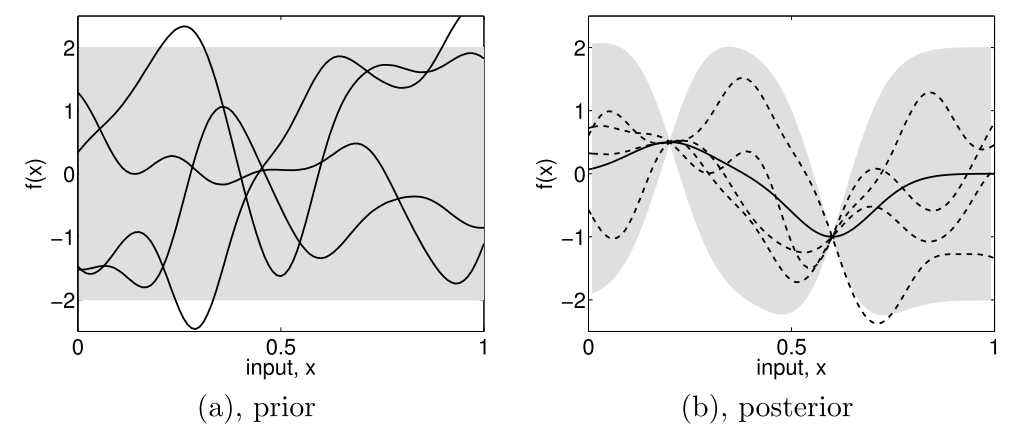
\includegraphics[width=\linewidth,keepaspectratio]{fig/literature/rasmussenGP.png}
\caption{Visualization of 4 Gaussian processes: \textbf{a} represents a sampling of the GP while in \textbf{b} these functions have been conditioned on two points. Shaded regions represent twice the standard deviation of the GPs. Source: \cite{rasmussen2006}.}
\label{fig:gp_prior-post}
\end{figure}

\bigskip
\subsection{Multifidelity}\label{sec:evofusion}

It is possible to combine several level of fidelity in order to lower the computational cost of the surrogate building process. The fidelity can be either expressed as a mesh difference, a convergence difference, or even a different set of solvers. Starting from~\cite{kennedy2000,kennedy2001}, there has been numerous studies on this topic---see these reviews~\cite{legratiet2013,peherstorfer2016,Fernandez2017}. All in all, multifidelity approaches are commonly used~\cite{padron2014,Wang2015,ahlfeld2016}.

In~\cite{courrier2016}, an extensive review of the principal methods is presented. They concluded that the approach proposed by \cite{forrester2006} was robust and performant. Their method uses a low fidelity model and corrects it using a model of the error:
\begin{align}
\mathcal{M}(x) = \mathcal{M}_c(x) + \mathcal{M}_{\epsilon}(Y_e(x), Y_c(x)),
\end{align}
\noindent with $\mathcal{M}_{\epsilon}$ the surrogate model representing the error between the two fidelity levels. For this method to perform optimally, nested design of experiments are required for the error model to be computed.

The process is explained in~\cref{fig:evofusion}. In this example, we seek to represent the model $\mathcal{M}_e$. We have at our disposal a limited number of evaluations $y_e$ of this model. Only using these sample produce a model which fails to predict the QoI for high values of the input parameter. On top of that, we have access to a model $Y_c$ with lots of samples due to its lower cost. Hence, we are able to predict with fidelity this model. Hence, the multifidelity approach allow to fix this low fidelity model with the few evaluations of the high fidelity model. This produces a surrogate model which exhibit the correct behaviour of the expensive model.

\begin{figure}[!ht]
\centering
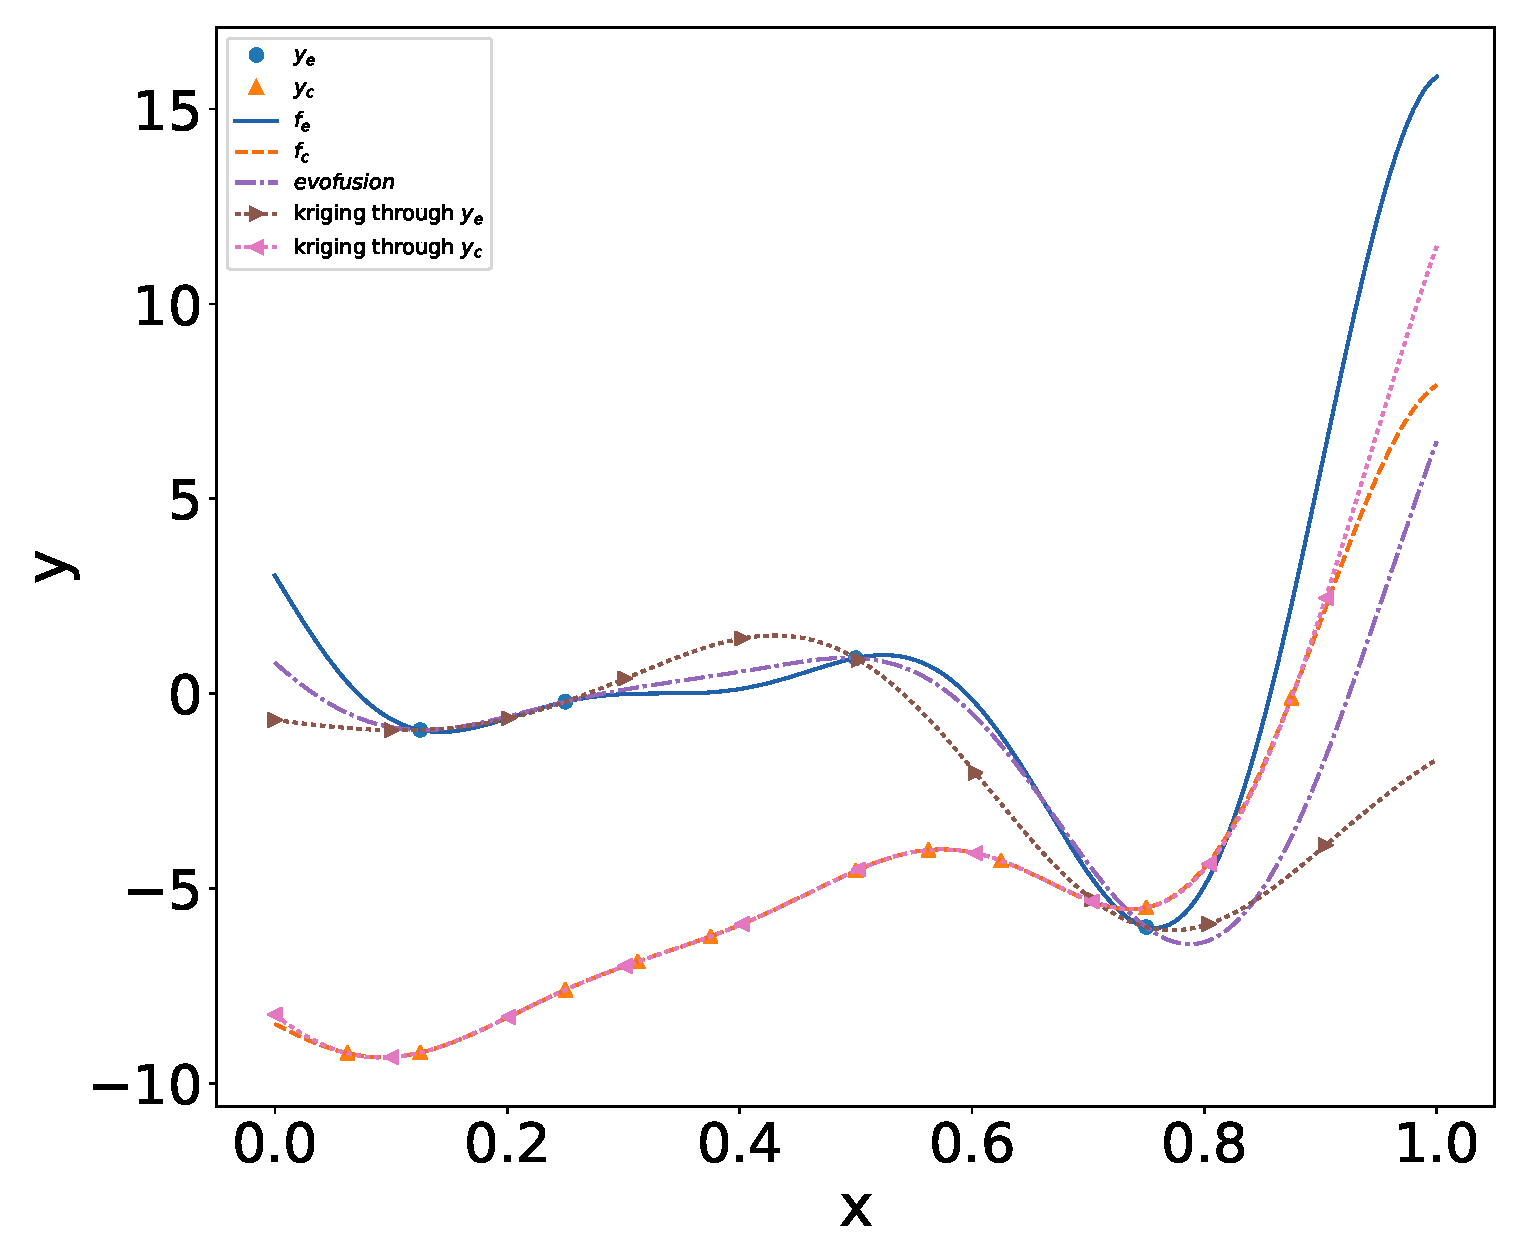
\includegraphics[width=0.8\linewidth,keepaspectratio]{fig/literature/evofusion_forrester.pdf}
\caption{Visualization of the multifidelity procedure on the analytical function of Forrester.}
\label{fig:evofusion}
\end{figure}

Considering two levels of fidelity $Y_e$ and $Y_c$, respectively an expensive and a cheap function expressed as a computational cost. A cost ratio $\alpha$ between the two can be defined as:
\begin{align}
\alpha = \frac{Y_e}{Y_c}.
\end{align}

Using this cost relationship an setting a computational budget $C$, it is possible to get a relation between the number of cheap and expensive realizations:
\begin{align}
C Y_e &= N_e Y_e + N_c Y_c,\\
C Y_e &= N_e Y_e + N_c\frac{\alpha}{Y_e},\\
C &= N_e + N_c\alpha, \\
N_c &= \frac{C - N_e}{\alpha}.
\end{align}

As the design being nested, the number of cheap experiments must be strictly superior to the number or expensive ones. Indeed, the opposite would result in no additional information to the system.

Multifidelity approaches have not been used in this thesis work as the focus was set on other aspects.

\subsection{Model Validation}\label{sec:validation}
An important step after having constructed a surrogate model is to assess its validity. There are lots of ways to do this and the common method consists in comparing with a metric the prediction of the model at a given point with the direct model output. The classical approach is to use a validation set which is different than the training set. This holdout procedure requires to split the entire dataset into two disjointed datasets---see~\cref{fig:validation}. There are no rules about the data sharing proportions. Things like the fitting time or the total number of samples lead to various splitting strategies. Depending on the number of simulations that can be afforded, the same dataset can be used to both construct the surrogate model and validate it. Independently of the strategy, various metrics can be used and common ones are given as follows. Note that only metrics used for regression are presented. The literature around classification metric is large and out of the scope of this work. 

\begin{figure}[!ht]
\centering
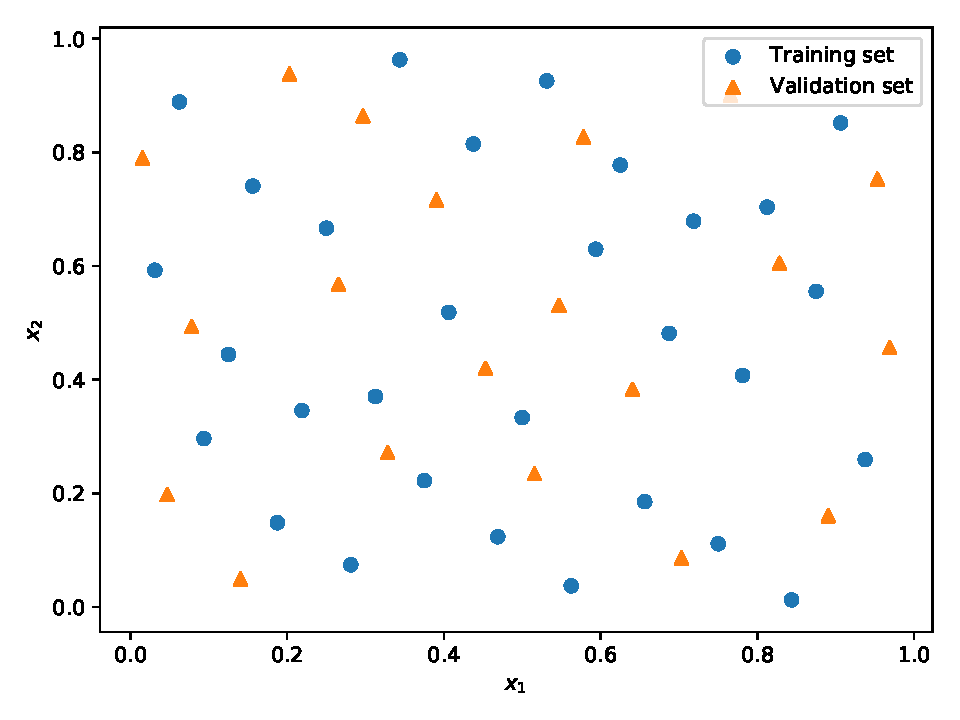
\includegraphics[width=0.7\linewidth,keepaspectratio]{fig/literature/validation_set.pdf}
\caption{3-dimensional parameter space canonical visualization of training (triangles) and validation (circles) sets.}
\label{fig:validation}
\end{figure}

\subsubsection{Mean Square Error and Alike}
Various metrics are used to compare the results of a known sample over the result of a prediction from a model. The Mean Square Error (MSE) basically computes the sum of the square differences. Taking its root allows conserving the dimensionality of the QoI
\begin{align}
\text{RMSE} = \sqrt{\frac{1}{N}\,
\displaystyle\sum_{i = 1}^{N}\,(Y_i - \hat{Y}_{i})^2}.
\end{align}
However, this method is not robust to outliers as one or two values can lead to large errors. Mean absolute error and median absolute error have a better behaviour toward this. In any case, the lower the error, the better the model.

\subsubsection{Coefficient of Determination: $Q_2$}
Another common indicator is the determination coefficient also called predictivity coefficient $Q_2$~\citep{marrel2009}. It is composed of both the mean square error and the variance of the output. It is a normalization of the MSE by the spread of the data. The variance normalization makes this indicator strictly lower than 1. This is handy for comparing models with each other as the QoI's units does not counts.
\begin{align} 
Q_{2} = 1 - \frac{\displaystyle\sum_{i = 1}^{N}\,\left(Y_i - \widehat{Y}_i\right)^2}{\displaystyle\sum_{i = 1}^{N}\,\left(Y_{i} - \overline{Y}_i\right)^2}.
\end{align}
A perfect model is characterized by a $Q_2=1$. With a constant model, $\hat{Y}$ is equal to the mean leading to $Q_2=0$. Finally, $Q_2=0$ can be negative, meaning that the model is arbitrary worse than a constant model.

\subsubsection{Kolmogorov-Smirnov Statistical Test}

The Kolmogorov-Smirnov test is a classical method used to evaluate the similarity between PDFs~\citep{clarke1992}. The difficulty of this method comes from the availability of the real PDF. Let $T_F$ (resp. $T_G$) be a random variable with cumulative distribution function (CDF) $F$ (resp. $G$). Let $F_n$ (resp. $G_m$) be its empirical CDF built from $n$ (resp. $m$) independent realizations of $T_F$ (resp. $T_G$). Then, let us define the test statistics:
\begin{align}
D = \sup_{x} \lvert F_n(x) - G_m(x)\rvert.
\end{align}
The null hypothesis for the Kolmogorov-Smirnov statistical test supposes that $T_F$ and $T_G$ are identically distributed, i.e.~$F=G$. The Kolmogorov-Smirnov test leads us to reject this hypothesis with a type I error $\alpha\in]0,1[$ when:
\begin{align}
D > c(\alpha)\,\sqrt{\frac{n+m}{nm}}, \label{eq:nullhypothesis}
\end{align}
with $c(\alpha)$ a tabulated value found in the literature~\citep{smirnov1939}. Considering $\alpha = 0.05$ and $n = m = N$, the null hypothesis is rejected if $D > \numprint{6.082e-3}$.

\subsubsection{Graphical Quality Assessment}
An easy way to visualize the quality of the model is to plot a joint plot. Its construction is simple. For a given sample, there is an observed value of QoI, let's say 5 (\cref{fig:qq_plot}). Then for the same sample, we take the predicted value of QoI, here also 5. These two values are used to construct a scatter plot. Thus, if the model is perfect, predicted values are equal to observed values leading to a line on this graph. On the right figure, the model is not as good as on the left, so an observed value of 5 is linked to a predicted value of 0.

A similar method consists in working on quantiles instead of absolute values of the output. Its interpretation is similar, a line would indicate a perfect fit.

\begin{figure}[!ht]
\centering
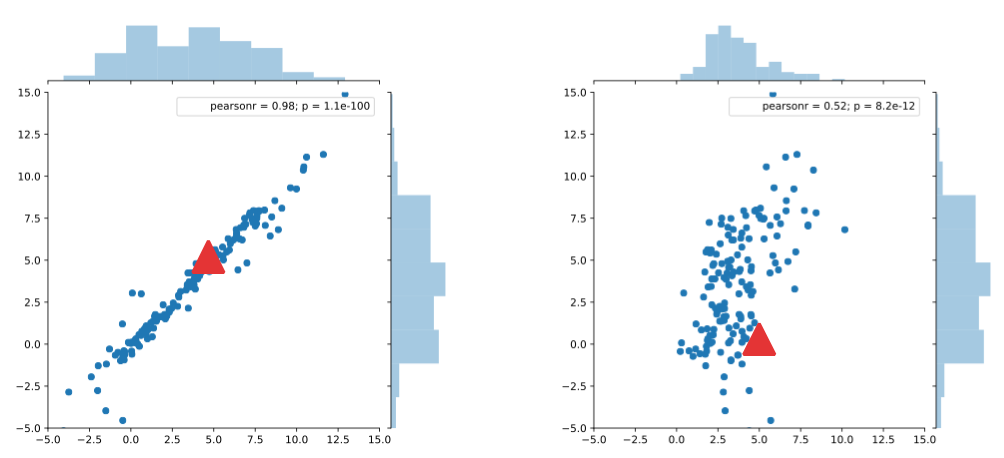
\includegraphics[width=\linewidth,keepaspectratio]{fig/literature/qq_plot.png}
\caption{Joint plot. QoI function of the predicted QoI given a parameter set. The triangle represents an observed value of 5.}
\label{fig:qq_plot}
\end{figure}

% TODO synthèse dans Barthelemy2017 de ROC etc.

\subsubsection{Holdout as Opposed to \emph{K-fold} or Cross Validation}
Another method is to keep the same sample set for both training and validation. It is called cross-validation or \emph{K-fold}~\cite{kohavi1995}. In this case, $K$ different models are constructed on subsets of the dataset and the metrics are computed on the points that are not used during the fitting of these different models. For \emph{K-fold} to work optimally, it assumes that the model is fairly stable to these points removal. In~\cref{fig:k_fold}, $K=3$ which leads to 3 subsets of 6 points being created. These 6 points are used for training a model while the other 3 points are used for computing a metric. These operations are repeated 3 times and all metrics results are aggregated. A particular case is found with $K$ being equal to the number of samples. This is called \emph{Leave-One-Out} (LOO).

\begin{figure}[!ht]
\centering

\includegraphics[width=0.6\linewidth,keepaspectratio]{fig/literature/k_fold.png}
\caption{Sketch of the \emph{K-fold} methodology. $K=3$ with $N=9$ which leads to 3 subsets of 6 points.}
\label{fig:k_fold}
\end{figure}


\section{Uncertainty Visualization}\label{sec:visu}
% Visualization issue
\lettrine{I}{n spite} of a wide literature on UQ, the community has yet to propose efficient ways to visualize uncertainties. Indeed, to the author's knowledge, there is no chapter dedicated to visualization in UQ reference books~\citep{Saltelli2007,sullivan2015,handbookUQ}. This remains to be investigated, especially for Computational Fluid Dynamics (CFD) and geosciences applications~\citep{Moreland2016} that involve complex fields of large dimensions. Classical ways of visualizing standard statistics can lead to misinterpretation~\citep{Anscombe1973}. The challenge for state-of-the-art visualization solutions stands in the dimension of the data. Assuming that the dimension of the data is limited (a set of scalars), for instance when dealing with input data, canonical subplots of subspaces are adapted. Parallel coordinate plots~\citep{Inselberg1985} or Kiviat plot (also referred to as the spider plot)~\citep{Hackstadt1994} that are represented in~\Cref{fig:sketch_Kiviat-parallel} offer an interesting alternative and share the same idea of dedicating one input variable (noted $x_i$) per axis; Kiviat (right panel) plot being the equivalent to parallel coordinates (left panel) plot in polar coordinates. 
\begin{figure}[!ht]
\centering
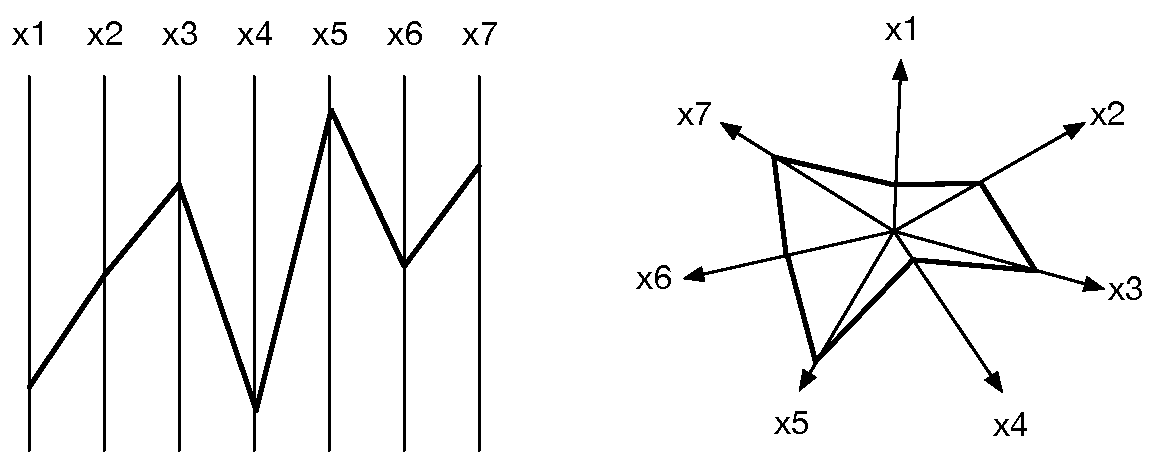
\includegraphics[width=0.9\linewidth,keepaspectratio]{fig/literature/parallel-kiviat.pdf}
\caption{Schematic representation of a parallel coordinate plot (\emph{left}) and a Kiviat plot (\emph{right}) for one sample.}
\label{fig:sketch_Kiviat-parallel}
\end{figure}
% Outputs

When the dimension of the data increases, for instance when dealing with \emph{functional} output fields discretized in both space and time on fine meshes, advanced strategies should be proposed. Different strategies are found in the literature to visualize statistics on the response variable~\citep{Potter2012a,Brodlie2012,Bonneau2014}. Beyond deterministic simulations, moving on to ensemble-based approaches, the dimension of the data further increases.

A first approach is to look at each realization of the data set individually, in the output space with curves, maps or 3D-graphs. In the early work of Sir Francis Galton and its bean machine, the sampling process illustrated the demonstration of the central limit theorem stating that the binomial distribution approximates the normal distribution. The animated version of the sampling procedure is referred to as the Hypothetical Outcome Plots (HOPs) technique~\citep{Ehlschlaeger1997} and was generalized by~\citep{Hullman2015} for a set of scalars as presented in~\cref{fig:pattern_hop}.

HOPs consists in animating a succession of possible outcomes sampled from the data. It was proven to enable the exploration and the understanding of the dataset general characteristic, even for people lacking statistical background~\citep{Belia2005} with the possibility to visually grasp correlations in the outputs. 

\begin{figure}[!ht]
\centering
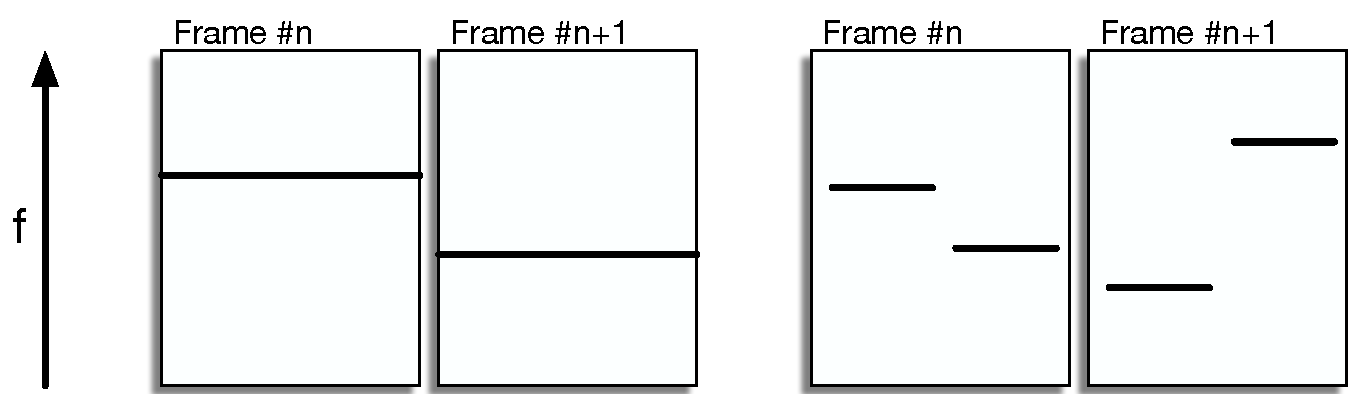
\includegraphics[width=0.9\linewidth,keepaspectratio]{fig/literature/pattern_hop.pdf}
\caption{Schematic representation of the HOPs method for single scalar output (\emph{left}) or multiple scalar outputs (\emph{right}).}
\label{fig:pattern_hop}
\end{figure}

Statistical moments and PDF plot are common tool for visualizing uncertainties in the context of ensemble simulation as illustrated in~\cref{fig:pattern_pdf}. They are useful for risk analysis as the probability of exceeding a threshold is directly observable. \Cref{fig:pattern_pdf}(a) displays the PDF for a scalar response variable (noted $f$) where the mean, the mode and extreme probabilities can be observed. \Cref{fig:pattern_pdf}(b) displays the principal mode of the PDF (solid black line) for a functional response variable discretized in the $x-$direction. The PDF standard deviation (added/removed to/from the mean) is plotted in dashed lines. These curves are computed for each $x$ independently and they do not represent a possible solution of the numerical solver. The box plot in \Cref{fig:pattern_pdf}(c) provides similar information while diminishing the false illusion of median/mean curves. It should be noted that users usually have a better understanding of frequency~\citep{Gigerenzer1995} than of PDFs and that there is a  general misinterpretation of confidence intervals~\citep{Belia2005}.
%augmenting 1-dimensional \emph{boxplot} visualizations 
\begin{figure}[!ht]
\centering
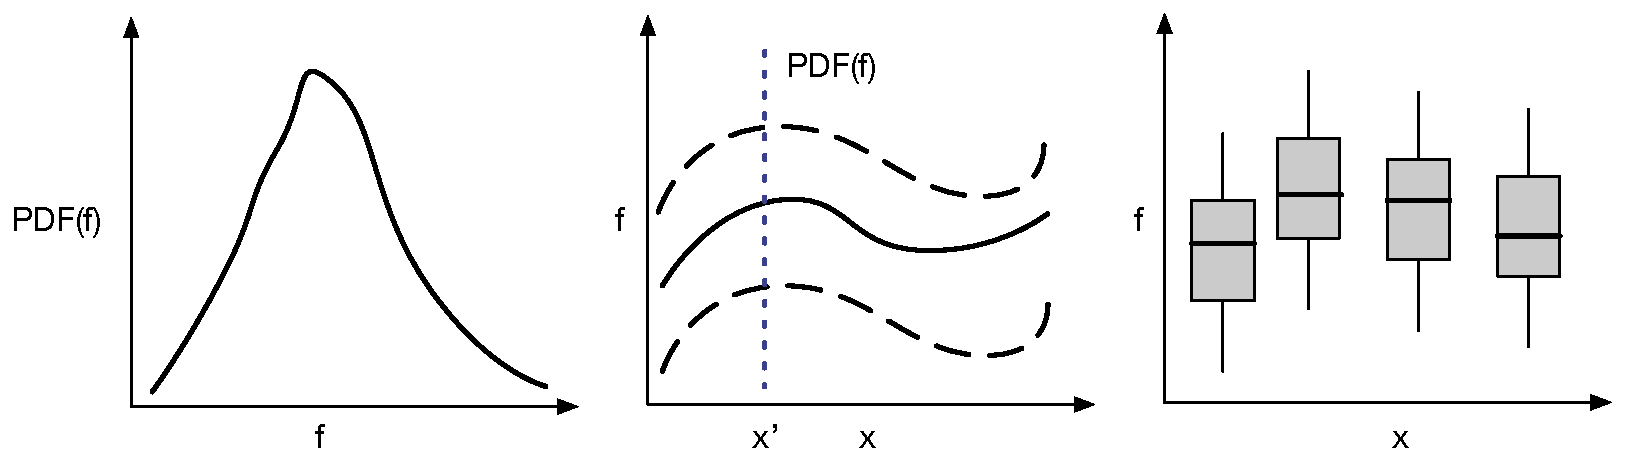
\includegraphics[width=\linewidth,keepaspectratio]{fig/literature/patterns_pdf.pdf}
\caption{Schematic representation of the PDF for a scalar output (\emph{left}), for a functional output (\emph{middle}) and with a boxplot solution (\emph{right}). The PDF mode is represented with a solid line, the standard deviation added/removed to/from the mean is represented with dashed lines.}
\label{fig:pattern_pdf}
\end{figure}

A complementary approach based on density criteria was proposed by~\citep{Hyndman2009,Sun2011}; it is noted HDR for Highest Density Region and represented in~\cref{fig:pattern_hdr}. It allows depicting some statistics (for instance median or outliers) taking into account the functional response variable as a whole and working in a reduced space (POD) spanned by the most significant directions of the output space. Within this reduced space, metrics for functional outputs are computed such as the distance to the median (blue curve) so that abnormal or outlier outputs (red and green curves) can be detected and quantiles can be estimated (blue envelope). Each curve represents either a realization within the data set or an additional realization sampled in the reduced space; thus functional characteristics such as spatial or temporal correlation are preserved.  From~\citep{Popelin2013,Ribes2015}, the HDR method is more robust to outlier detection than other methods such as functional boxplot~\citep{Sun2011,Whitaker2013}.

\begin{figure}[!ht]
\centering
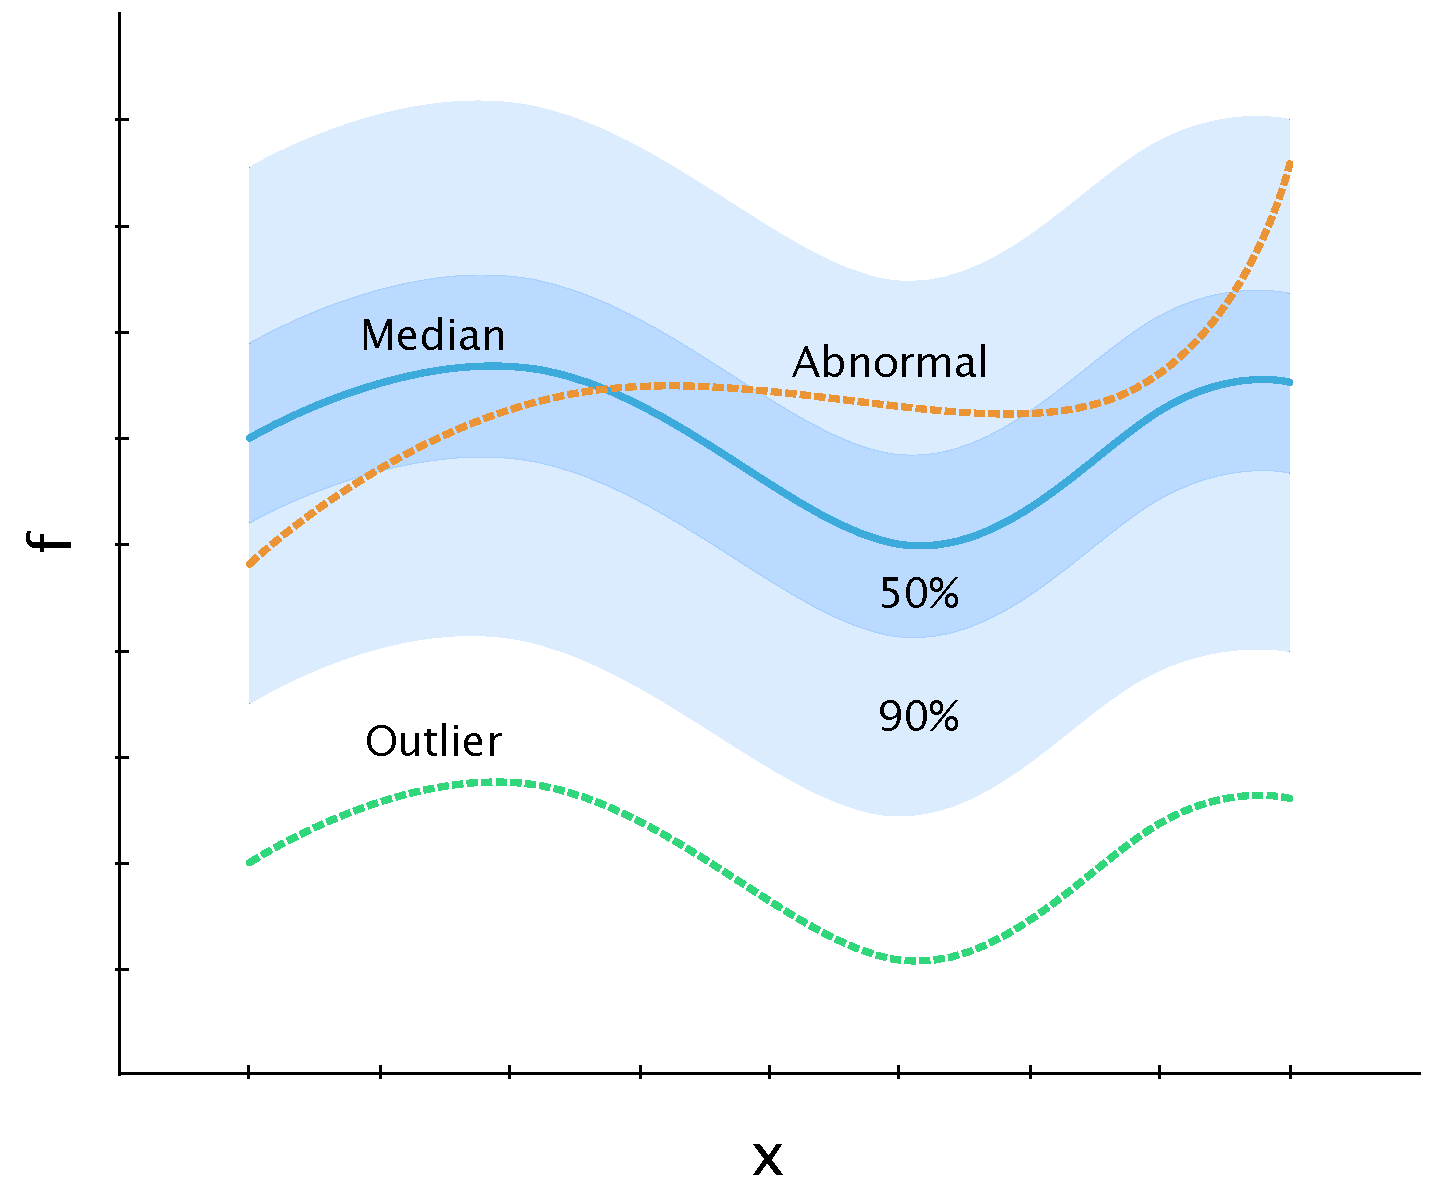
\includegraphics[width=0.6\linewidth,keepaspectratio]{fig/literature/pattern_hdr.pdf}
\caption{Schematic representation of data set functional realizations characterized with HDR metrics. The median is represented by the solid blue line, the abnormal and outliers are represented by the red and green lines and the 50\% and 90\% quantiles are represented by blue shaded envelopes.}
\label{fig:pattern_hdr}
\end{figure}

\subsection{Highest Density Region}
\label{sec:HDR}

The dataset output is considered as a matrix where each line corresponds to a realization. This matrix is decomposed by POD. The modes are ordered by decreasing importance in terms of contribution to the variance and only a finite number of modes are kept. In this reduced space, the functional dataset of large dimensions is conveniently represented by a limited number of scalars mapped onto most significant directions that maximizes the variance of the response variable. Within this reduced space, the classification of different patterns or the computation of metrics is eased~\citep{Ren2017}. Hence, within this reduced space, the median realization corresponds to the HDR location. The distance to this point is computed in the modal space; the further a point is from the HDR, the less probable is the realization~\footnote{The term \emph{median}, which is used in the literature, is restrictive if there are multiple clusters of point in the reduced space.}.

A multivariate KDE (see~\cref{sec:up}) technique is used to estimate the PDF $\hat{f}(\mathbf{x_r})$ of this multivariate space. From this KDE, the HDR reads
\begin{align}
R_\alpha = {x_r: \hat{f}(\mathbf{x_r}) \geq f_{\alpha}},
\end{align}
\noindent with $f_{\alpha}$ such that $\int_{R_\alpha} \hat{f}(\mathbf{x_r}) d x_r = 1 - \alpha$. With this definition, the HDR corresponds to the region of highest PDF with a cumulative probability of $1-\alpha$. The 50\% and 90\% HDR are computed, corresponding respectively to $\alpha=0.5$ and $\alpha=0.1$. By construction  a HDR develops around the maximum PDF $\max \{\hat{f}(\mathbf{x_r})\}$ which identifies the most probable mode. Transposed using the inverse transform from the reduced space to the original space, this most probable mode corresponds to the "central curve"---also referred to as the median curve. 

Except if the response variable of the system of interest is chaotic under the perturbation of its input parameters, the POD is expected to drastically reduce the dimensionality of the problem. Furthermore, as the system's response variable is also expected to oscillate around some modes, the points in the reduced space are likely to be relatively clustered around the modes. This mitigates the difficulty of the density estimation procedure.

\begin{figure*}[!ht]               
\centering
\subfloat[]{
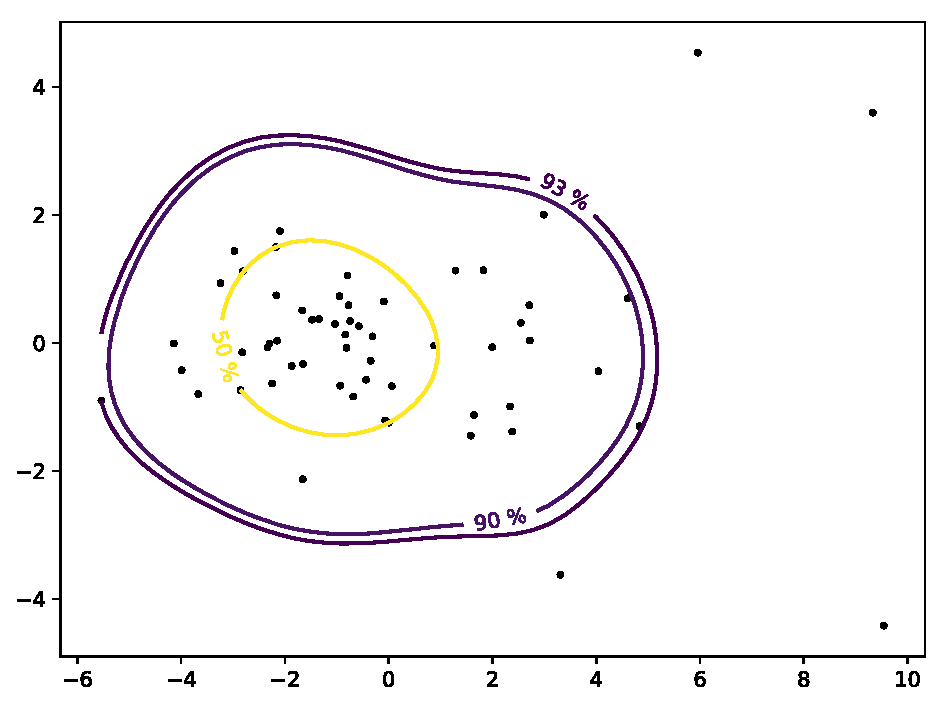
\includegraphics[width=0.47\linewidth,height=\textheight,keepaspectratio]{fig/contributions/visu/hdr_scatter.pdf}}
\subfloat[]{
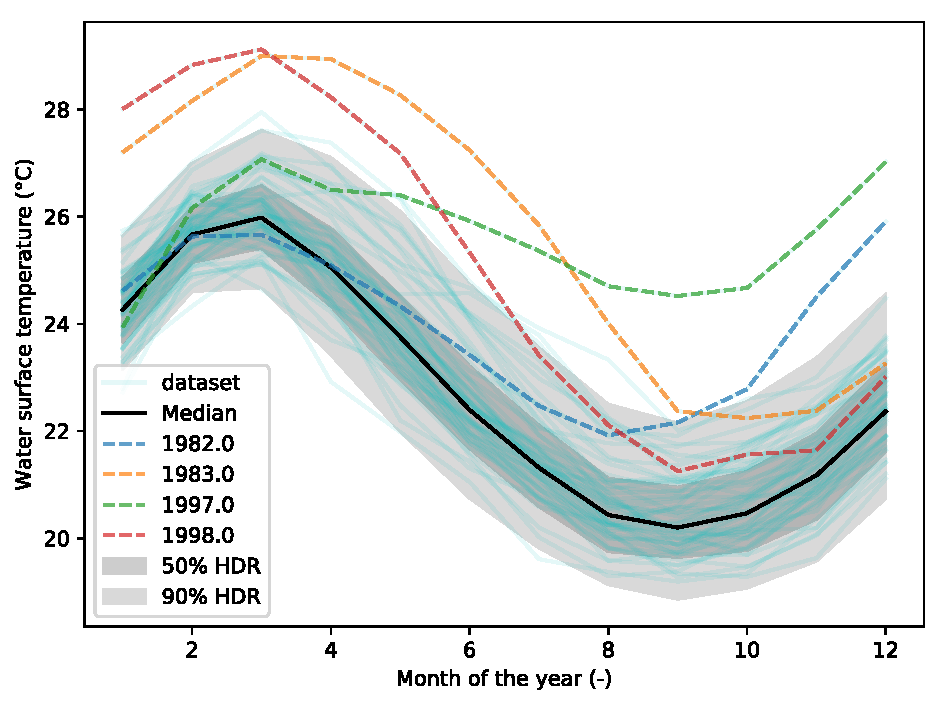
\includegraphics[width=0.47\linewidth,height=\textheight,keepaspectratio]{fig/contributions/visu/hdr_curves.pdf}} 
\caption{HDR boxplot on the El Ni\~no dataset. \textbf{a} scatter plot of the 2-dimensional reduced space with each dot as a realization. \textbf{b} dataset visualization with each curve as a realization from the database. Shaded areas are confidence intervals, \emph{thick solid black} line is the mean realization and \emph{highlighted-dashed} curves are outliers.}
\label{fig:elnino}
\end{figure*}

\cref{fig:elnino} illustrates the HDR boxplot for the El Ni\~no dataset in the reduced space \emph{(left)} when only two modes are retained ensuring that at least 80\% of the response variable variance is conserved. Each realization is characterized with respect to the HDR metric. In the modal space, each dot represents a realization within the dataset and the contouring represents the 50\% and 90\% quantiles. In the response variable physical space (\emph{right}), \emph{cyan curves} represent the realizations from the dataset, the outliers are \emph{coloured-dashed curves}, the \emph{thick black curve} is the median and the \emph{grey shaded areas} represent 50\% and 90\% quantiles envelopes. It should be noted that additional realizations with chosen characteristics on the outputs could be drawn by sampling the input for specific HDR criteria.


%\section{Software}\label{sec:software}



\chapter{Scientific Questions}\label{chap:questions}

\lettrine{F}{rom} this literature review, this thesis proposes to contribute to three axis:

\begin{itemize}
\item \emph{How to construct a DoE in a high-dimensional parameter space?}\hfill\\
	The number of simulations at hand is highly constrained by the computational power, the cost and the return time. A surrogate can only interpolate the physics which has already been seen, hence the need to explore uniformly the parameter space. When the number of parameters is high, controlling the sparsity in the DoE is challenging. I have developed a new sampling strategy that is versatile and performs well with such constrains.
	
\item \emph{How to resample a DoE by considering the QoI of already sampled experiments?}\hfill\\
	Using the aforementioned novel method, it is possible to iteratively complete the DoE. This method does not incorporate any prior information on the shape of the response of the system. Here I propose a method which combines a Gaussian Process surrogate model with a LOOCV procedure in order to add a new sample in the DoE. This method has proven good behaviour in high-dimensional parameter space.

\item \emph{How to visualize uncertainties in high-dimensional cases?}\hfill\\
    Analysing both input parameter space and QoI is challenging when the dimension is high. I present some new ways to help understand uncertainties in this context.
\end{itemize}

To support these methodological aspects, some industrial applications have been used.




\end{parttoc}

\part{Scientific Contributions}
\begin{parttoc}
    \chapter{Batman}

\section{Description}
Bayesian Analysis Tool for Modelling and uncertAinty quaNtification (batman) is an open source Python package dedicated to statistical analysis based on non-intrusive ensemble experiment.

\emph{batman} library provides a convenient, modular and efficient framework for design of experiments, surrogate model and uncertainty quantification. *batman* relies on open source python packages dedicated to statistics (*openTURNS* and *scikit-learn* [@openturns, @scikit-learn]). It also implements advanced methods for resampling, robust optimization and uncertainty visualization [@roy2017a].

*batman* handles the workflow for statistical analysis. It makes the most of HPC resources by managing asynchronous parallel tasks. The internal parallelism of each task does not conflict with *batman*'s parallel environment.

*batman* analysis is launched from a *command line interface* and a setting file. *batman* functionalities can also be accessed through an API.

*batman* is CECILL-B licensed; it is actively developed and maintained by researchers at CERFACS.

\section{Implementation}



\section{Dissemination}


\chapter{Constructing a Design of Experiments}
\section{Presentation of the method}\label{sec:method}

In its basis form, our adaptive sampling strategy consists in adding a point far from the existing points in the parameter space. The notion of distance corresponds to a measure of discrepancy. However, instead of considering the whole hypercube, the technique proposed only focuses on empty regions defined using an Exclusion Field (EF). This exclusion field describes the probability of selecting a new point depending on its position.

By means of utilizing EF, it becomes possible to generate new samples that are located preferentially in these empty regions. Then, out of the $n_{gen}$ generated samples from the EF, the one that leads to the best value of some criterion is selected. It is to be noted that there is no optimization process in the sense that it is just a selection process based on probable samples of the EF. The whole process ensures randomness in the generation of the parameter space. Its algorithm is shown in~\cref{alg:doe}. %Hereafter, this method is referred to as the KDOE method.

\Cref{sec:kde} introduces the EF, and \cref{sec:sample} describes the sampling procedure from the EF. Agorithm \ref{alg:doe} gives an overview of the method. In the following, it is referred to as the Kernel-DoE (KDOE) method. 

\begin{algorithm}
  \caption{Sampling Strategy: Kernel-DoE}
  \label{alg:doe}
  \begin{algorithmic}[1]
  \Require $\mathbf{X}^{N_s}_d$, $N_{max}$, $N_s$, $n_{gen}$
  \Comment{Start from a sample $\mathbf{X}^{N_s}_d$ composed of $N_s$ samples in dimension $d$}
  \While{$N_s < N_{max}$}
    \State $f \gets$ Construction of the Exclusions Field from $\mathbf{X}^{N_s}_d$
    \State $\mathbf{Y}^{n_{gen}}_d \gets$ pick $n_{gen}$ samples using Metropolis-Hasting MCMC
    \State $\mathbf{Y}^{j}_d \gets$ point in $N_{gen}$ which minimize the discrepancy
	\State $\mathbf{X}^{N_s + 1}_d \gets \left\{\mathbf{X}^{N_s}_d, \mathbf{Y}^{j}_d \right\}$
  \EndWhile
  \end{algorithmic}
\end{algorithm}




\subsection{Determination of the exclusion field}\label{sec:kde}

It is assumed that there are $N_s$ samples that have already been selected. The spatial probability density function used to draw a new sample is given by:
\begin{align}
f(\mathbf{x}) &= 1 - \sum_{i=1}^{N_{s}} K\left(\mathbf{x},\mathbf{x}^{(i)}\right) \, .
\end{align}
The $N_s$ samples that have already been chosen are noted $\mathbf{x}^{(i)}$, with $i$ between 1 and $N_s$. The dimension is noted $d$ and $K$ is a kernel expressed by:
\begin{align}
K\left(\mathbf{x},\mathbf{x}^{(i)}\right) = \exp\left( - \frac{D\left(\mathbf{x},\mathbf{x}^{(i)}\right)^2}{2h^2} \right),
\end{align}
$D$ is a distance function expressed latter. The general idea is to reduce the probability of selecting a new point close to the samples already drawn. Hence a zone of exclusion is created around each of the already selected points, with a width parametrized by $h$. The parameter $h$ has been set to $h = \frac{\sigma}{N_s^{1/d}}$ with $\sigma=0.3$. This allows us to have a width of exclusion that decreases as the number of samples increases.

Moreover, the probability is set to 0 outside of the unit hypercube in order to prevent sampling outside of the region of interest. Note that this probability is not normalized. This is not a problem because the sampling procedure does not requires this property, as it will be shown in the next section.

The expression of the distance function $D$ is used to generate many different shapes. In our case, alignment of samples on each axis should be avoided as done with Latin Hypercube Sampling designs. This is achieved by using a Minkowski distance~\citep{Cha2007} for $D$:
\begin{align}
D\left(\mathbf{x},\mathbf{x}^{(i)}\right)=\left(\sum_{j=1}^d |x_{j}-x_{ij}|^p\right)^{1/p},
\end{align}
where $p$ is the order of the distance. Setting $p < 1$ leads to a \emph{star shape}, as shown in~\cref{fig:minkowsky} where one sample has already been selected. In the following, $p=0.5$ is used. In~\cref{fig:3d_kde}, three samples have already been selected. The star shape is present in all dimensions. Moreover, these shapes interact with each other as they cross as shown in \cref{fig:inter_kde}. In this case $\sigma=0.8$ to highlight this property.

\begin{figure}[!h]               
\centering
%\subfloat[Wrap-around discrepancy]{
%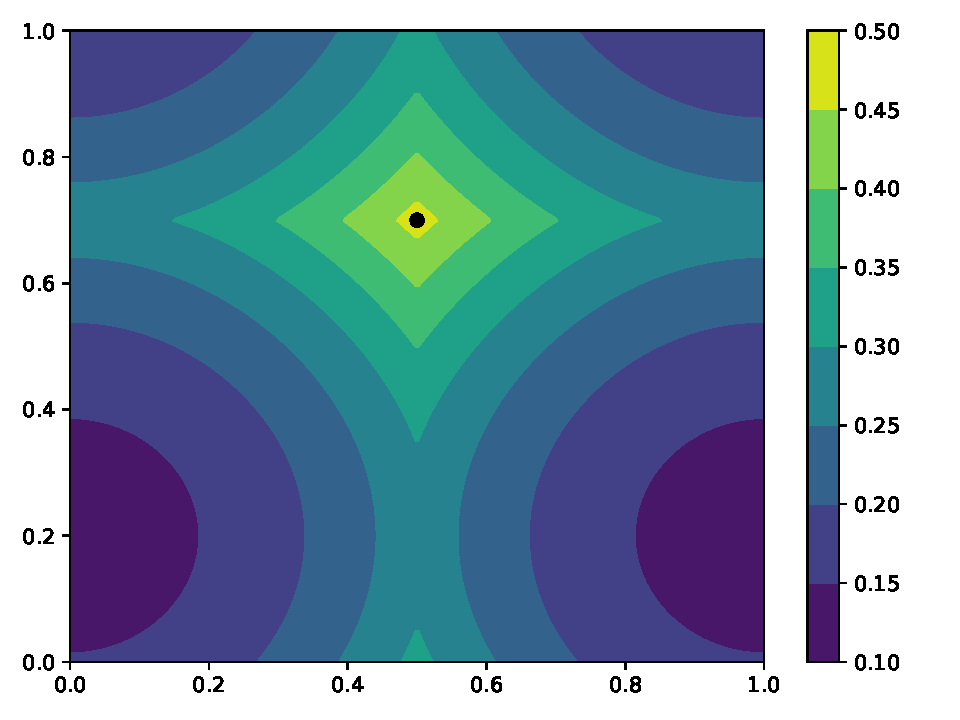
\includegraphics[width=0.49\linewidth,height=\textheight,keepaspectratio]{fig/contributions/doe/wrap_disc.pdf}}
%~
%\subfloat[Inverse Mindkowsky distance]{
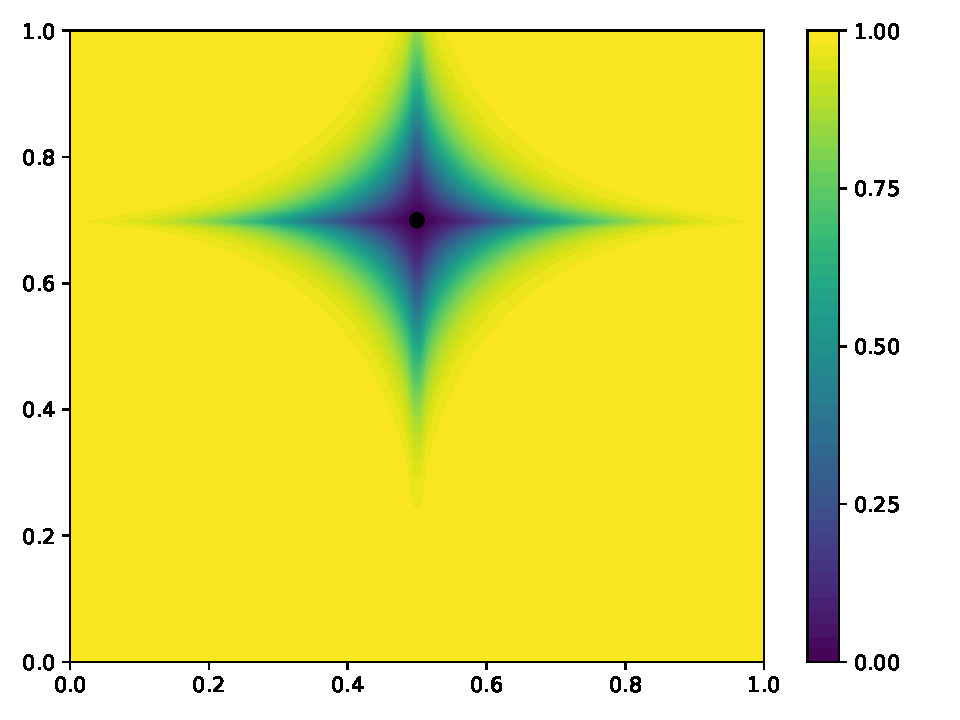
\includegraphics[width=0.8\linewidth,height=\textheight,keepaspectratio]{fig/contributions/doe/inv_minkowsky.pdf}
%}
\caption{Probability density in a 2-dimensional parameter space. \emph{Dot} represents the sample already drawn at (0.5, 0.7).}
 \label{fig:minkowsky}
\end{figure}

\begin{figure}[!h]
\centering
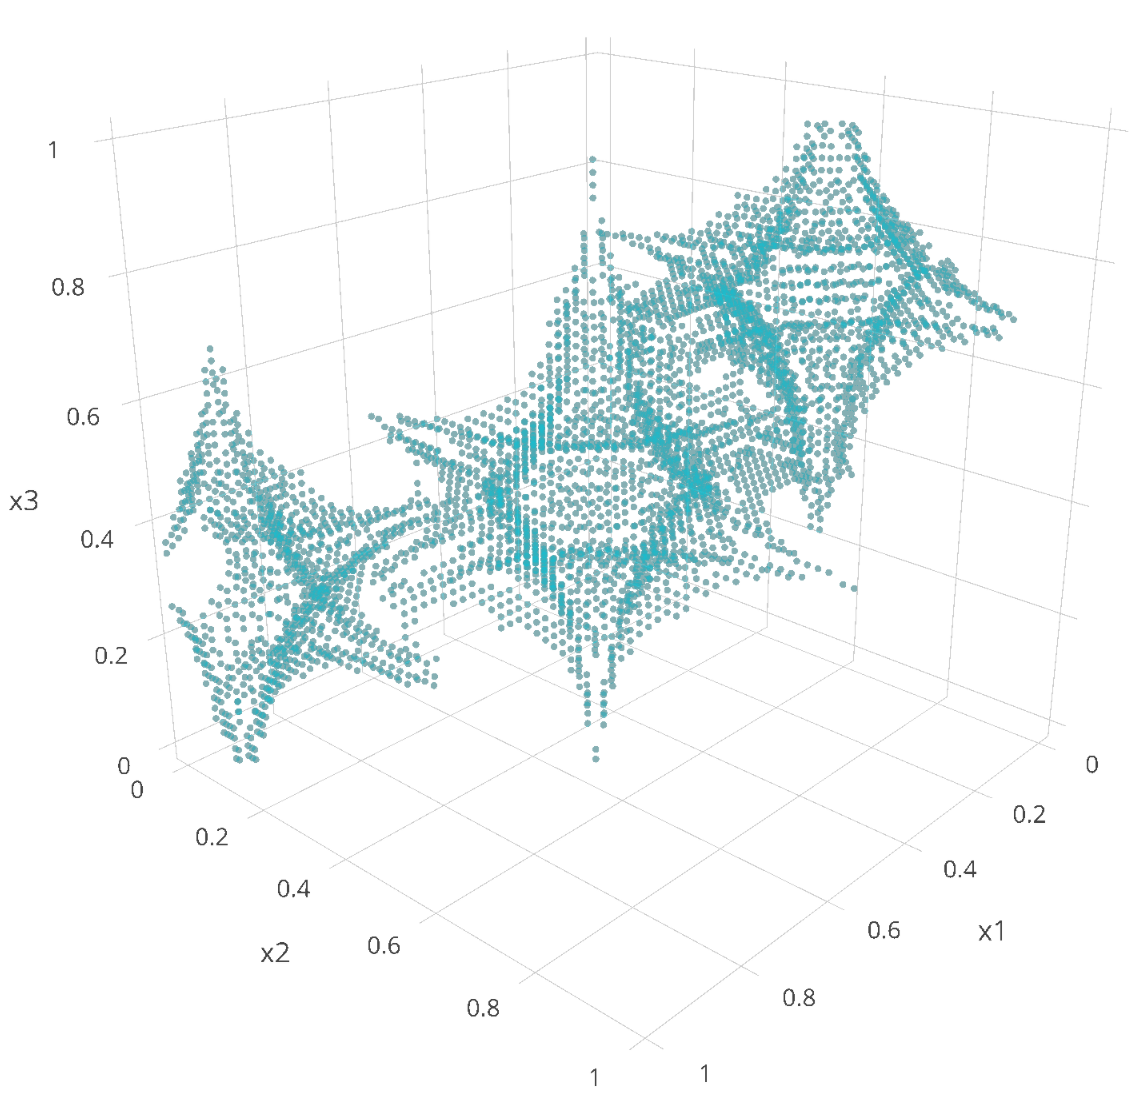
\includegraphics[width=0.8\linewidth,keepaspectratio]{fig/contributions/doe/3d_star.png}
\caption{Scatter plot representation of a 3-dimensional KDE with three points in the parameter space. Points represents an iso contour of probability.}
\label{fig:3d_kde}
\end{figure}

\cleardoublepage

\begin{figure}[!h]
\centering
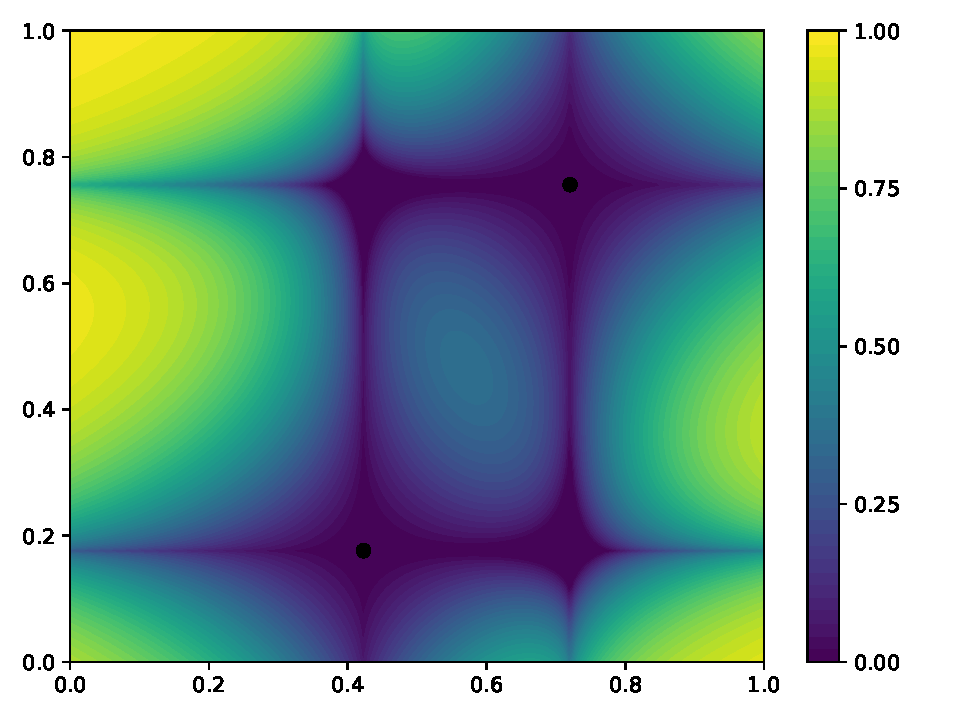
\includegraphics[width=0.8\linewidth,keepaspectratio]{fig/contributions/doe/kde_inter.pdf}
\caption{Interaction effects on the probability density in a 2-dimensional parameter space. \emph{Dots} represent 2 existing samples.}
\label{fig:inter_kde}
\end{figure}




\subsection{Sampling and selection procedures}\label{sec:sample}

%Using the modified version of the KDE, it is possible to generate samples following the posterior distribution.

The classical way to sample from a PDF is to use the inverse transform sampling method. However, finding the inverse cumulative distribution function of a complex PDF can be computationally intensive ---\thinspace the cost increases with dimensionality. The \emph{Metropolis-Hasting}~\citep{Hastings1979} algorithm was selected as an efficient way to sample from $f$. Contrary to methods such as HMC or NUTS~\citep{Hoffman2011}, it does not require the calculation of the gradient of the log-probability density function, which is a costly operation. This algorithm provides a random walk of the parameter space that converges toward the target PDF.

%Using an arbitrary distribution $g(\mathbf{x}|\mathbf{y})$, a new candidate $\mathbf{x}$ is evaluated based on the previous point $\mathbf{y}$. This property makes it a \emph{Markov Chain} as the current value is only conditioned by the previous one. The distribution $g$ is chosen as a Gaussian PDF so that samples close to the previous one are preferably sampled. This algorithm provides a random walk of the parameter space that converges toward the target PDF.


\Cref{fig:sample_kde} shows an example with two initial points already selected in the hypercube $[0, 1]^2$. Based on these two points (\emph{dots}), $f$ is build and new samples are drawn (\emph{squares}).

\begin{figure}[!h]
\centering
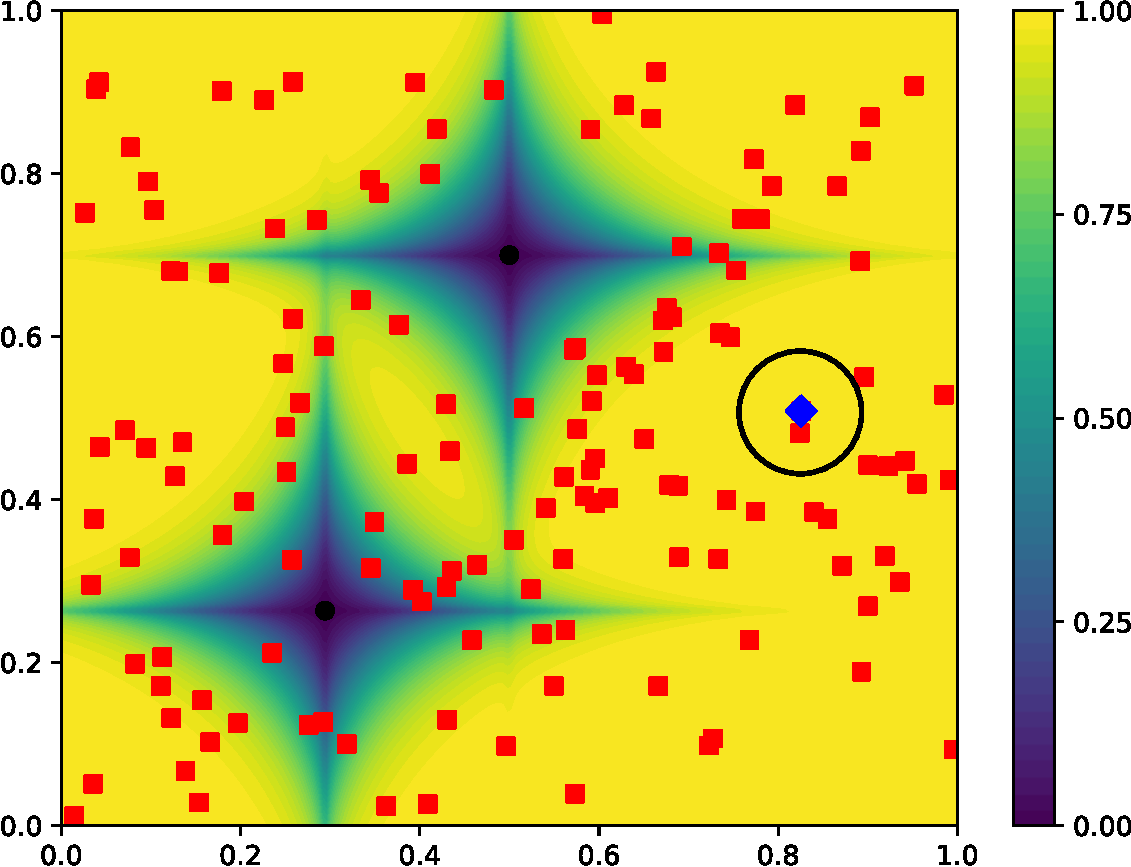
\includegraphics[width=0.7\linewidth,keepaspectratio]{fig/contributions/doe/sampling_KDE.pdf}
\caption{Probability density in a 2-dimensional parameter space. \emph{Dots} represent the samples already drawn, \emph{squares} are the result of the Metropolis-Hasting sampling and \emph{circled-diamond} is the sample selected based on the resulting centred discrepancy.}
\label{fig:sample_kde}
\end{figure}

The next step consists in choosing a new sample from these candidates. Any metric can be chosen here depending on the final objective. In the following, we focused on the uniformity of the DoE. Hence, the centred discrepancy $C^2$ is used~\citep{Fang2006}. It writes
\begin{align}
C^2(\mathbf{X}^{N_s}_d) =& \left( \frac{13}{12} \right)^d - \frac{2}{N_s}\displaystyle\sum_{i=1}^{N_s}\prod_{k=1}^{d} \left( 1 + \frac{1}{2} \mid  x_k^{(i)} - 0.5\mid - \frac{1}{2} \mid  x_k^{(i)} - 0.5\mid^2\right)\\ \nonumber
& + \frac{1}{N_s^2}\sum_{i,j=1}^{N_s}\prod_{k=1}^d \left( 1 + \frac{1}{2} \mid  x_k^{(i)} - 0.5\mid + \frac{1}{2} \mid  x_k^{(j)} - 0.5\mid - \frac{1}{2} \mid  x_k^{(i)} - x_k^{(j)}\mid \right).
\end{align}




\noindent Since the lowest values of $C^2$-discrepancy result in more uniform samples, the sample minimizing it is chosen (\emph{circled-diamond}). Thus, this iterative procedure acts like and optimizer on the $C^2$-discrepancy where the candidates are not drawn totally randomly but with the knowledge of the current samples. 

%TODO : COMPRENDS PAS : LE COUT EST A CHAQUE NOUVEAU TIRAGE The cost of the method is concentrated at the KDE step. Once the KDE is computed, sampling candidates and choosing the next sample is computationally inexpensive.

%\Cref{fig:star} shows an example with 10 points. The initial sample consisted of one point. The result is a low discrepancy sample constructed iteratively.

The method is not deterministic which is useful if one wants to generate a new independent set of experiments. To compute sensitivity indices of \emph{Sobol'}, two independent samples are required~\citep{Saltelli2010}. As stated in~\citep{Saltelli2010}, quasi-random sequences such as \emph{Sobol'} are classically used but, as they are deterministic, it is not possible to generate an independent sample directly. One possibility is to get these two samples as one sample of shape $X_{2d}^{N_s}$. Splitting the matrix column wise-like ensures independence of the samples. However, as the dimensionality increases, the quality of the sequence deteriorates ($d > 10$). Hence, this technique is limited to a small number of dimensions. Our method does not share this limitation.

%\begin{figure}[!h]
%\centering
%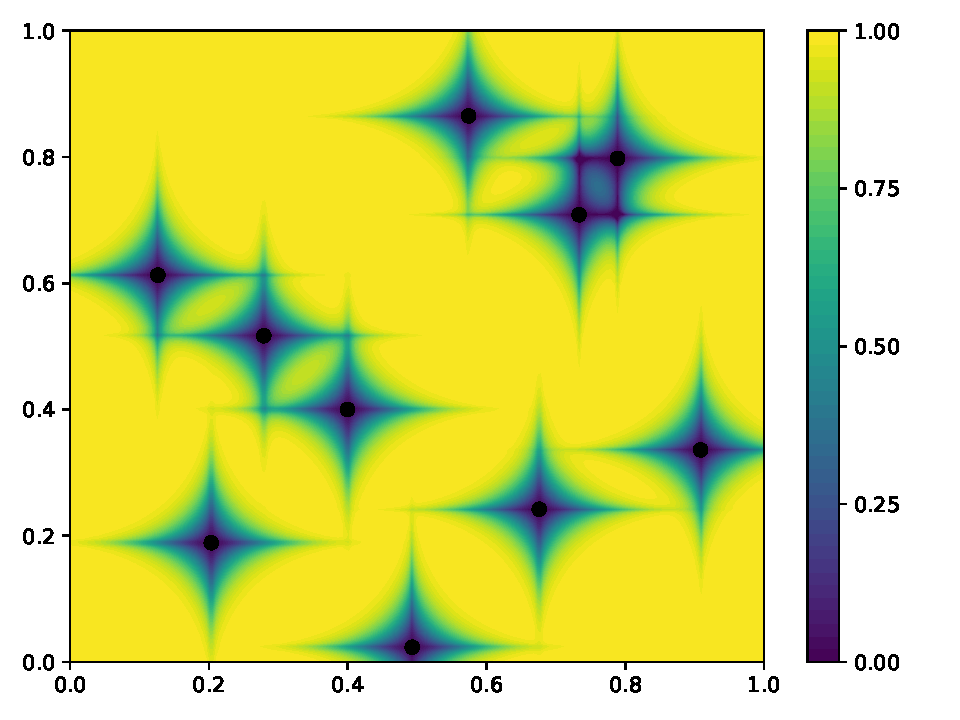
\includegraphics[width=0.9\linewidth,keepaspectratio]{fig/contributions/doe/10_star.pdf}
%\caption{Probability density in a 2-dimensional parameter space. The 10 \emph{dots} represent the samples used to fit the KDE.}
%\label{fig:star}
%\end{figure}

As stated, $n_{gen}$ candidate samples are generated through MCMC. \Cref{fig:conv-ngen} presents a convergence analysis of the quality of the final design $X_2^{40}$ depending on the size of the MCMC sample at each iteration. Confidence intervals are calculated using 100 realizations of the same parametrization. The discrepancy converges to its final value after $n_{gen}>100$. This allows to control the computational cost required to generate the DoE. Various configurations of $X_d^{N_s}$ have been tested and results are similar. In the following, $n_{gen}$ was fixed to 100.

\begin{figure}[!h]
\centering
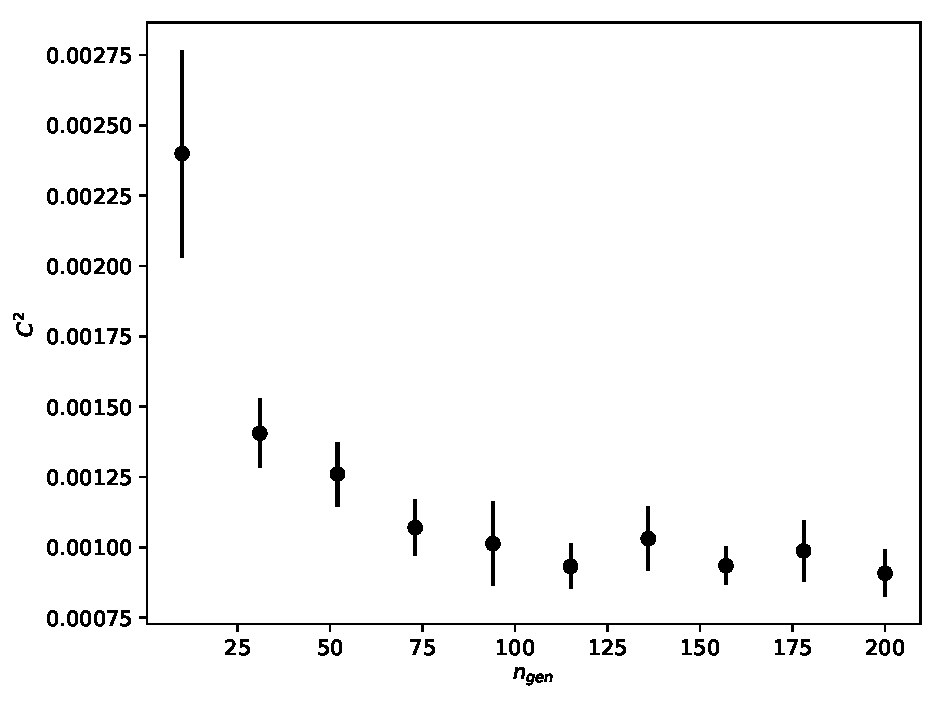
\includegraphics[width=0.9\linewidth,keepaspectratio]{fig/contributions/doe/conv_C2-Ngen-Kdoe2-40.pdf}
\caption{Convergence of the $C^2$-discrepancy function of $n_{gen}$ the size of sample using Metropolis-Hasting for $X_2^{40}$.}
\label{fig:conv-ngen}
\end{figure}


% TODO also good for multifidelity designs


% TODO property A, B with star. Do plot

%\newpage
\section{Results}\label{sec:results}

\subsection{Uniformity of the Design}
As stated previously, the uniformity of the DoE is paramount to ensure that the physics of interest are well captured. \Cref{fig:conv-dim-ns} presents a convergence study of the KDOE method versus \emph{Sobol'} sequences~\citep{Sobol1967}, classical LHS~\citep{Mckay1979}, and optimized LHS as proposed in~\citep{Baudin2015a}. Each point corresponds to a given sample size $N_s$ for a given number of dimensions $n_{dim}$. Due to the stochastic nature of the LHS algorithms and of the KDOE, confidence intervals are computed based on 100 realizations. To measure the improvement of a method with respect to one another, the $C^2$-discrepancy is used~\citep{Fang2006,Androulakis2016} and values are normalized by crude \emph{Monte Carlo} results. This transformation shows that a uniform improvement factor is obtained in comparison to MC. Looking for instance at $n_{dim} = 20$, LHS enables a 20\% improvement in terms of $C^2$-discrepancy over MC, \emph{Sobol'} sequence gives 30\% and both OLHS and KDOE roughly give 40\%.

Looking only at the contestants' methods, their hierarchy is quite stable. OLHS is the best method followed by \emph{Sobol'} sequence and finally LHS. For KDOE, it performs closely to \emph{Sobol'} sequence up to $n_{dim} \lesssim 20$. For $n_{dim} \gtrsim 20$, KDOE performs better than the other methods tested. Moving on to the standard deviation at $2\sigma$ ---\thinspace see~\cref{fig:conv-dim-ns_err}\thinspace---, the variation of the $C^2$-discrepancy is contained between LHS’s and OLHS’s.

\newpage
\begin{figure}[!h]               
\centering
\subfloat[]{
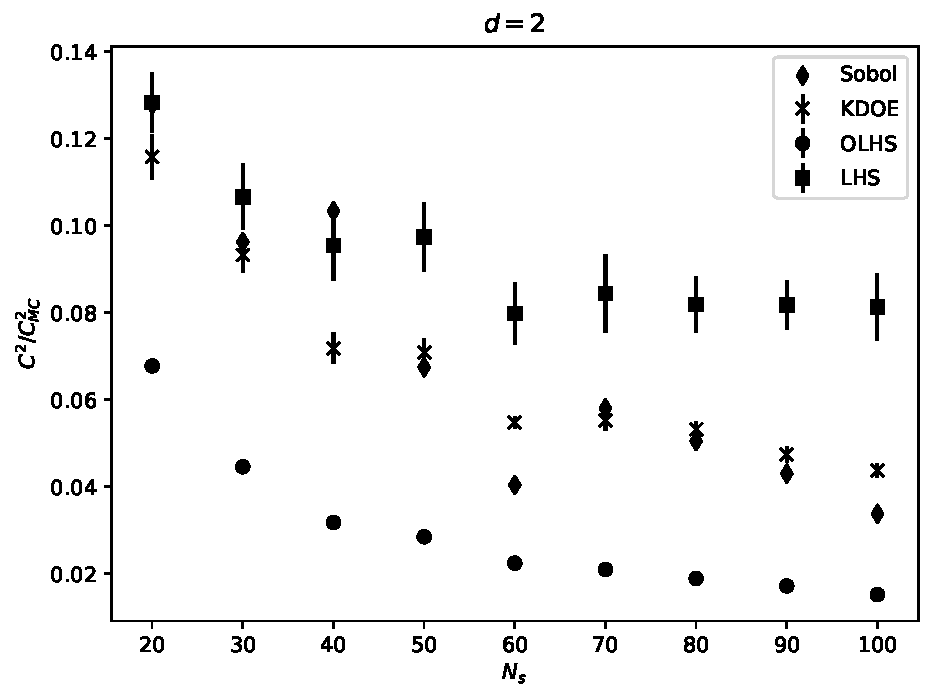
\includegraphics[width=0.48\linewidth,height=\textheight,keepaspectratio]{fig/contributions/doe/kde_2_C.pdf}}
 ~       
\subfloat[]{
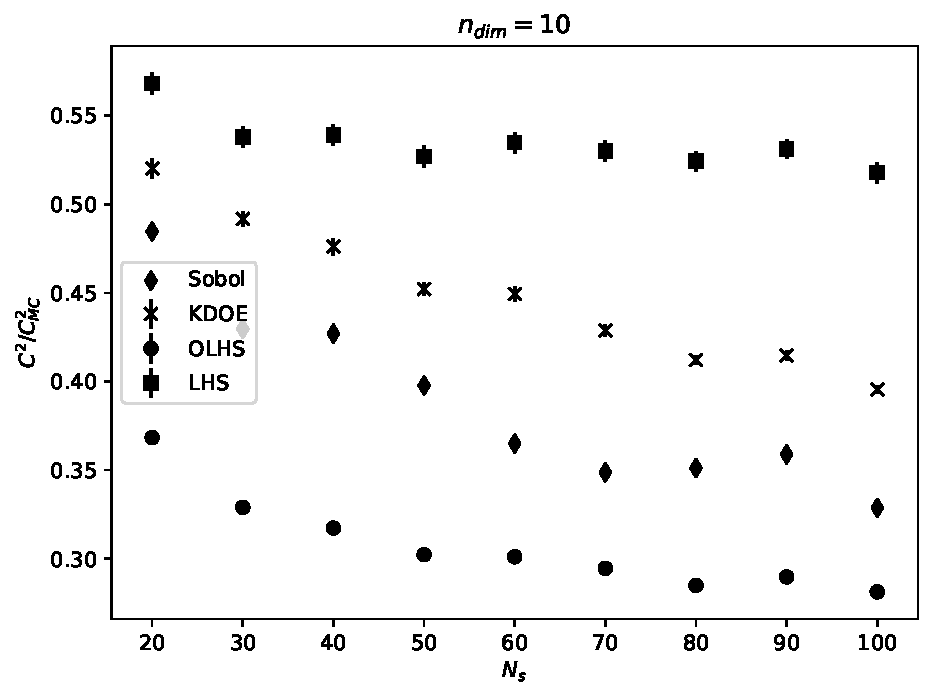
\includegraphics[width=0.48\linewidth,height=\textheight,keepaspectratio]{fig/contributions/doe/kde_10_C.pdf}}

\subfloat[]{
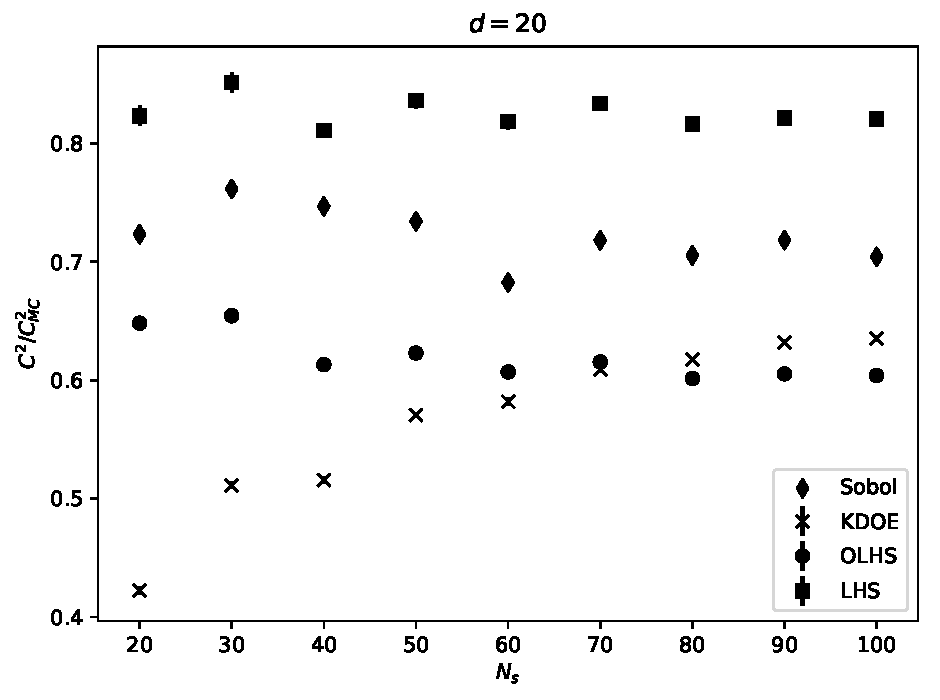
\includegraphics[width=0.48\linewidth,height=\textheight,keepaspectratio]{fig/contributions/doe/kde_20_C.pdf}}
 ~       
\subfloat[]{
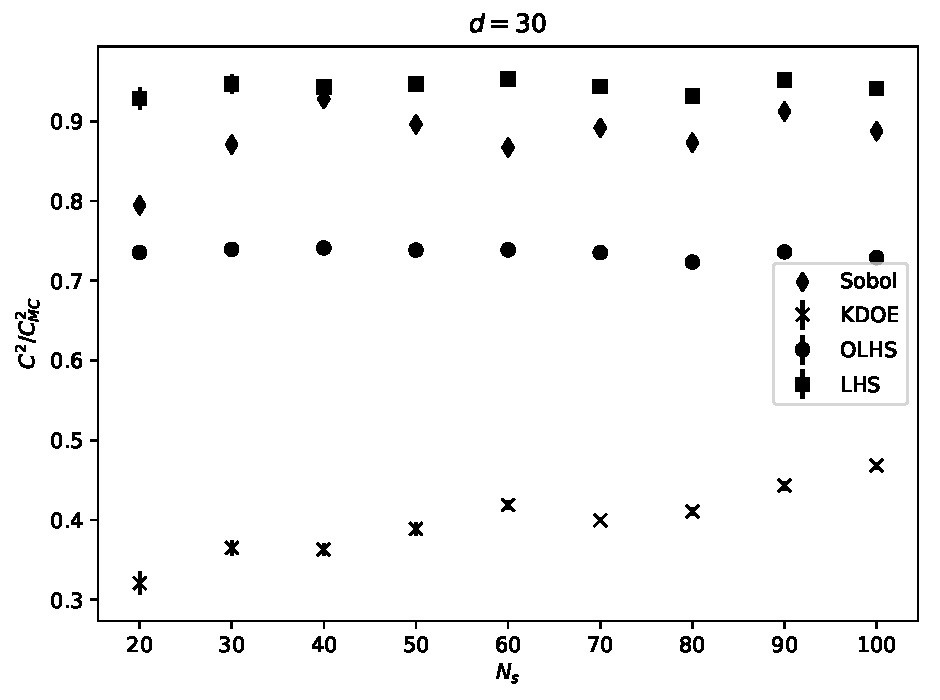
\includegraphics[width=0.48\linewidth,height=\textheight,keepaspectratio]{fig/contributions/doe/kde_30_C.pdf}}
\caption{Adimonsionalized $C^2$-discrepancy function of the number of dimensions $n_{dim}$ of the parameter space and of the size $N_s$ of the design for various DoE methods.}
\label{fig:conv-dim-ns}
\end{figure}
\begin{figure}[!h]               
\centering
\subfloat[]{
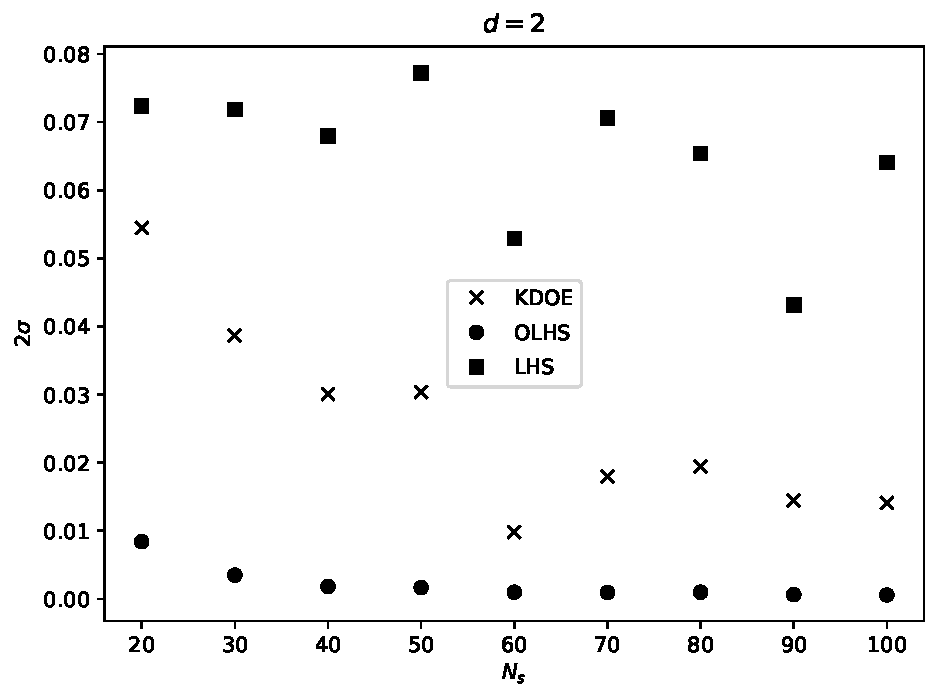
\includegraphics[width=0.48\linewidth,height=\textheight,keepaspectratio]{fig/contributions/doe/kde_err_2_C.pdf}}
 ~       
\subfloat[]{
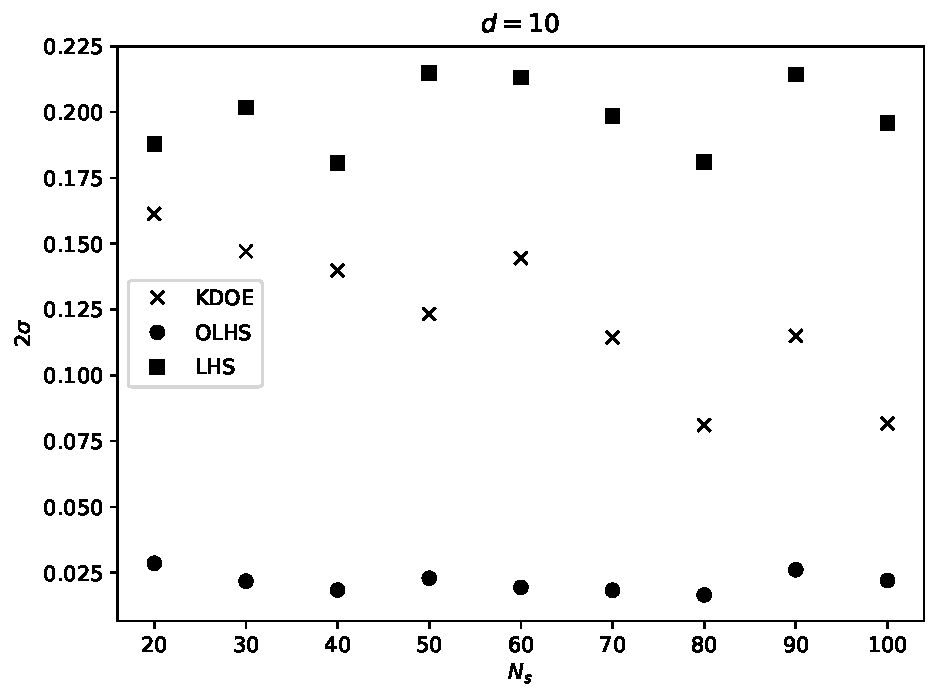
\includegraphics[width=0.48\linewidth,height=\textheight,keepaspectratio]{fig/contributions/doe/kde_err_10_C.pdf}}

\subfloat[]{
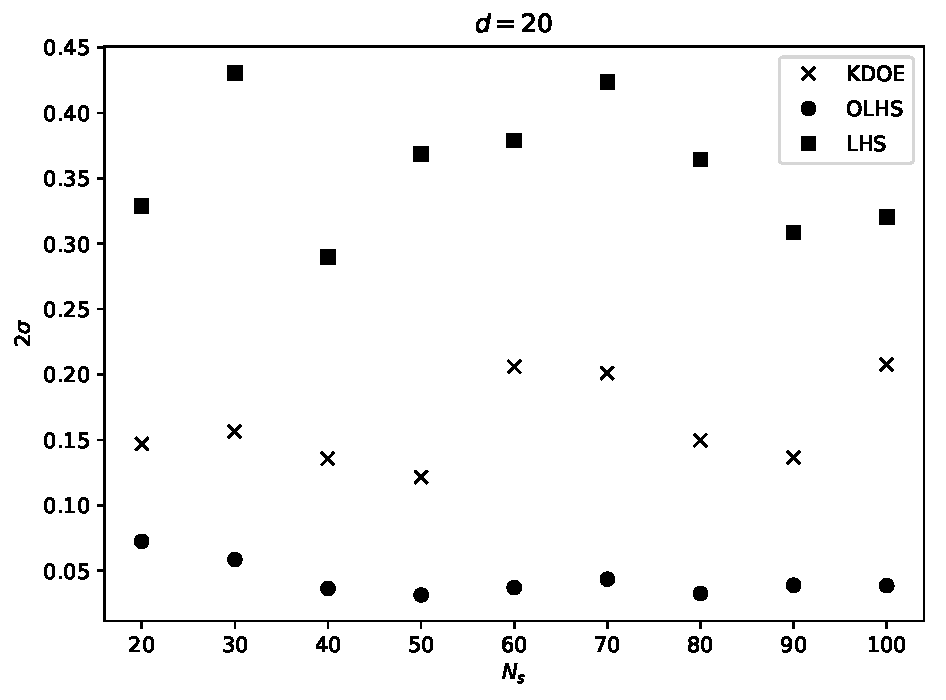
\includegraphics[width=0.48\linewidth,height=\textheight,keepaspectratio]{fig/contributions/doe/kde_err_20_C.pdf}}
 ~       
\subfloat[]{
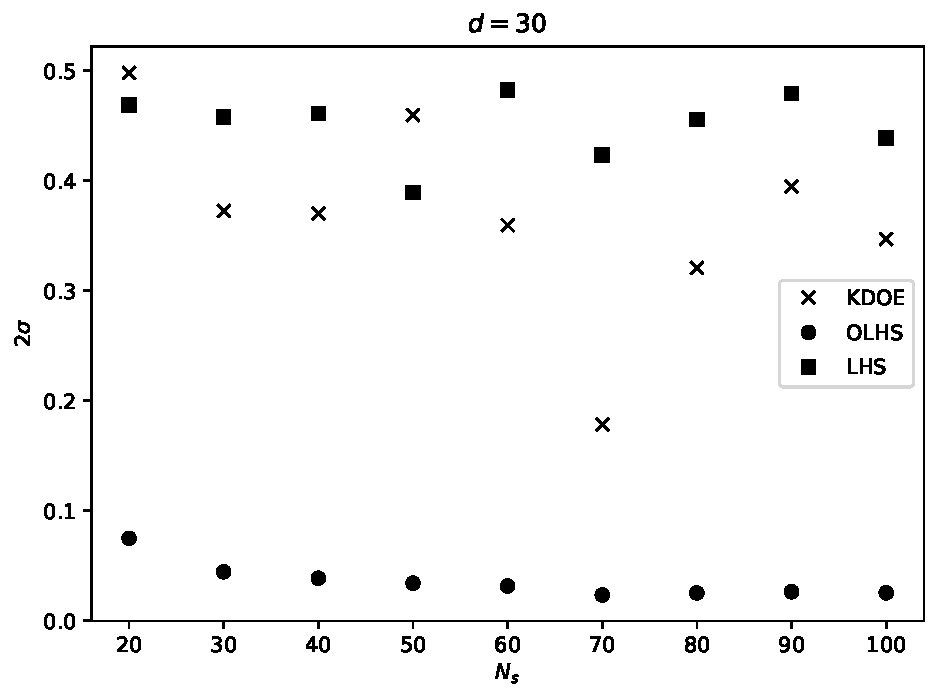
\includegraphics[width=0.48\linewidth,height=\textheight,keepaspectratio]{fig/contributions/doe/kde_err_30_C.pdf}}
\caption{Adimonsionalized $2\sigma$ deviation on the $C^2$-discrepancy function of the number of dimensions $n_{dim}$ of the parameter space and of the size $N_s$ of the design for various DoE methods.}
\label{fig:conv-dim-ns_err}
\end{figure}

\newpage


\Cref{fig:conv-dim-100} presents the convergence analysis of the $C^2$-discrepancy as function of the number of dimensions for $N_s = 100$. When the dimensionality increases, the gain with both LHS and \emph{Sobol'} sequences is close to zero. On the contrary, OLHS seems to stabilize around a 30\% improvement. Regarding KDOE, it performs equally with other methods up to $n_{dim} \lesssim 20$, while for $n_{dim} \gtrsim 20$ it becomes more performant. It can be seen that the method has yet to converge at $n_{dim} = 40$.

\begin{figure}[!h]
\centering
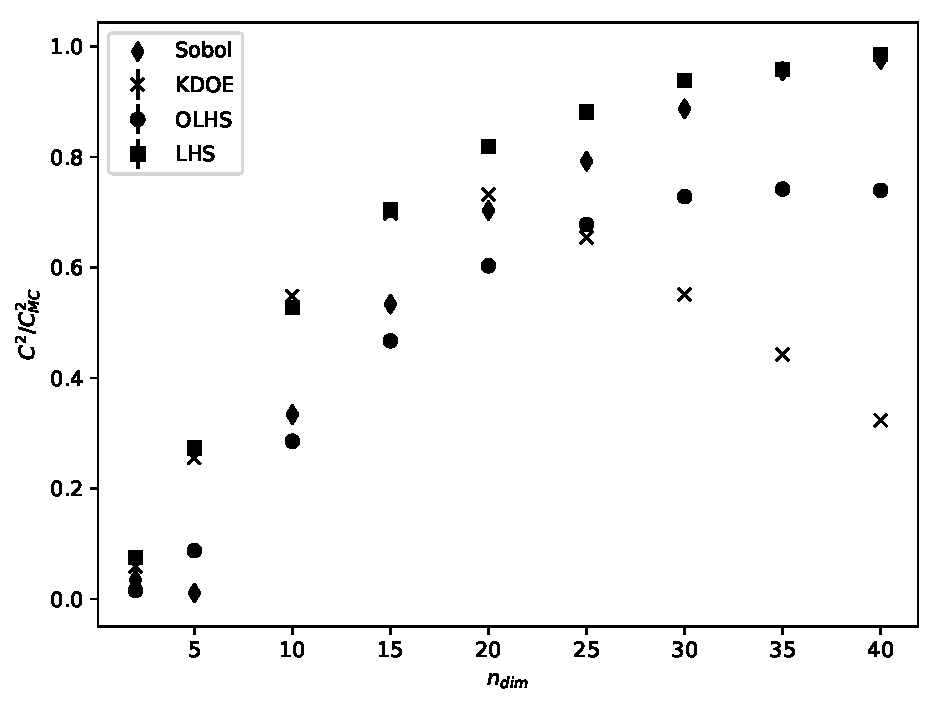
\includegraphics[width=0.9\linewidth,keepaspectratio]{fig/contributions/doe/kde_dim.pdf}
\caption{Adimonsionalized $C^2$ discrepancy function of the number of dimensions $n_{dim}$ of the parameter space with a design of size $N_s = 100$ for various DoE methods.}
\label{fig:conv-dim-100}
\end{figure}

In terms of $C^2$-discrepancy, KDOE appears to perform better with respect to crude \emph{Monte Carlo}, LHS, OLHS and \emph{Sobol'} sequence. \Cref{fig:comp-subspace} shows an example of a sample of size $N_s = 50$ in dimension $n_{dim}=30$. The subprojection $x_{20}/x_8$ is represented. \Cref{fig:comp-subspace}(d) depicts the principal challenge with classical \emph{Sobol'} sequences. In high dimensional parameter space, clear patterns may appear in some subprojections. This behaviour was not observed with KDOE. In this case, the result of the KDOE may not appear optimized for 2-dimensional subprojections. This is due to the fact that the objective is to optimize the total discrepancy of the parameter space.

%C^2\left(\mathbf{X}^{N_s}_{d}
\begin{figure}[!h]               
\centering
\subfloat[KDOE---$C^2=2.18$]{
\includegraphics[width=0.47\linewidth,height=\textheight,keepaspectratio]{fig/contributions/doe/20_8_kde.pdf}}
 ~       
\subfloat[OLHS---$C^2=3.43$]{
\includegraphics[width=0.47\linewidth,height=\textheight,keepaspectratio]{fig/contributions/doe/20_8_olhs.pdf}}

\subfloat[LHS---$C^2=3.81$]{
\includegraphics[width=0.47\linewidth,height=\textheight,keepaspectratio]{fig/contributions/doe/20_8_lhs.pdf}}
 ~       
\subfloat[Sobol'---$C^2=3.76$]{
\includegraphics[width=0.47\linewidth,height=\textheight,keepaspectratio]{fig/contributions/doe/20_8_sobol.pdf}}
\caption{Example of a 2-dimensional subprojection of the sample of size $N_s=50$ in dimension $n_{dim}=30$.}
\label{fig:comp-subspace}
\end{figure}


\subsection{Integration Convergence}

Even if this method is not designed for integral evaluation, its performance is evaluated on small numbers of samples up to 512. The number of evaluations has been restricted as the purpose of the method is to generate a small design in high dimensions. Also, the use of an iterative method to generate such sample can be questioned due to the resulting computational cost. Moreover, although this method can be used to continue an existing design created using another technique, such possibility was not evaluated in the following. In~\citep{Kucherenko2015}, convergence plots are presented in order to assess the performance of \emph{Sobol'} sequence versus LHS and \emph{Monte-Carlo} sampling. The functions used are categorized into types A, B and C. These categories state how the variables are important with respect to the function output:
\begin{description}
\item[Type A:] Functions with a low number of important variables,
\item[Type B:] Functions with almost equally important variables but with low interactions with each other,
\item[Type C:] Functions with almost equally important variables and with high interactions with each other.
\end{description}
Type C functions represent the most challenging case. In this work, one function per group is considered as detailed in~\cref{tab:conv_int}. The theoretical integral for all these function in the unit hypercube is 1. Quality of the integration is computed using the Root Mean Square Error (RMSE) defined as
\begin{align}
\epsilon = \left( \frac{1}{K} \displaystyle \sum_{k=1}^{K} \left(I[f] - I_{N_s}^k [f]\right)^2 \right)^{1/2},
\end{align}
\noindent with $K=50$ the number of independent trials and the estimate integral defined as
\begin{align}
I_{N_s}^k [f] = \frac{1}{N_s} \sum_{i=1}^{N_s} f(\mathbf{X}^{i}_d),
\end{align}
\noindent with $f$ the function to integrate. %In each case, the RMSE's evolution is approximated by $cN_s^\alpha$, with $0 < \alpha < 1$ the rate of convergence.

\begin{table}[!h]
\centering
\caption{Type A, B and C functions used in the convergence analysis.}
\begin{tabular}{clc}
\toprule
Type &  Function $f(x)$ & Dim $n$\\
 &   &  \\
\midrule % \cmidrule{2-3}
A & $\displaystyle\prod_{i=1}^n \frac{\mid 4x_i - 2 \mid + a_i}{1 + a_i}$& 30\\
B & $\displaystyle\prod_{i=1}^n \frac{n-x_i}{n-0.5}$ & 30\\
C & $2^n \displaystyle\prod_{i=1}^n x_i$ & 10\\
\bottomrule
\end{tabular}
\label{tab:conv_int}
\end{table}

%\begin{table}[!h]
%\centering
%\caption{Convergence results for type A, B and C functions.}
%\begin{tabular}{clccccc}
%\toprule
%Type &  Function $f(x)$ & Dim $n$ & \multicolumn{4}{c}{Slope $\alpha$} \\
% &   &  & MC & LHS & \emph{Sobol'} & KDOE\\
%\midrule % \cmidrule{2-3}
%A & $\displaystyle\prod_{i=1}^n \frac{\mid 4x_i - 2 \mid + a_i}{1 + a_i}$ & 30 & 0.55 & 0.55 & 0.42& 0.42\\
%B & $\displaystyle\prod_{i=1}^n \frac{n-x_i}{n-0.5}$ & 30 & 0.48& 0.66& 0.46& 0.72\\
%C & $2^n \displaystyle\prod_{i=1}^n x_i$& 10 & 0.47& 0.47& 0.31& 0.39\\
%\bottomrule
%\end{tabular}
%\label{tab:conv_int}
%\end{table}

\Cref{fig:conv_int} presents the convergence study. KDOE is not the best method but seems to compare to both LHS and \emph{Sobol'} sequence. The convergence rates are correct for every function type.


\begin{figure}[!h]               
\centering
\subfloat[Type A]{
\includegraphics[width=0.6\linewidth,height=\textheight,keepaspectratio]{fig/contributions/doe/kde_int_2A.pdf}}
   
\subfloat[Type B]{
\includegraphics[width=0.6\linewidth,height=\textheight,keepaspectratio]{fig/contributions/doe/kde_int_1B.pdf}}

\subfloat[Type C]{
\includegraphics[width=0.6\linewidth,height=\textheight,keepaspectratio]{fig/contributions/doe/kde_int_2C.pdf}}
\caption{RMSE function of the sample size $N_s$ for type A, B and C functions. The trend line corresponds to the RMSE evolution for Monte Carlo's method.}
\label{fig:conv_int}
\end{figure}

\cleardoublepage

\section{Perspectives}

Depending on the property sought, the combination of a Kernel and a metric allows an infinite customization of the method.

Using the Minkowsky distance as a metric, the LHS constrain is not strict which can be useful when dealing with discrete parameters. Indeed, strict LHS would prevent having more than one sample per discreet parameter. In~\cref{fig:lhs_const}(a), an additional constrain is added to strongly limit the probability to 0 when the $L_{-\infty}$-norm is inferior to a threshold. This limitation can be restricted to a domain of influence using an additional $L_2$-norm constrain (\cref{fig:lhs_const}(b)). Hence, this method acts as an iterative LHS strategy.



\begin{figure}[!h]               
\centering
\subfloat[Inverse Mindkowsky distance with LHS properties]{
\includegraphics[width=0.49\linewidth,height=\textheight,keepaspectratio]{fig/contributions/doe/kde_minkowsky_LHS.pdf}}
~
\subfloat[Inverse Mindkowsky distance with LHS properties and constrain]{
\includegraphics[width=0.49\linewidth,height=\textheight,keepaspectratio]{fig/contributions/doe/kde_minkowsky_LHS-const.pdf}}

\caption{Probability density in a 2-dimensional parameter space. \emph{Dot} represents the sample used to fit the KDE.}
 \label{fig:lhs_const}
\end{figure}

%\begin{figure}[!h]
%\centering
%\includegraphics[width=0.9\linewidth,keepaspectratio]{fig/contributions/doe/kde_constrain.pdf}
%\caption{Probability density in a non-rectangular 2-dimensional parameter space. \emph{Dot} represents the sample used to fit the KDE.}
%\label{fig:const_kde}
%\end{figure}


Using this method, it is also possible to consider non-rectangular domains~\citep{Lekivetz2015}. This example presents a 2-dimensional domain with the constrain $0.5 < x_1 \times x_2 < 1$. In this case, the selection of the point criterion has to be changed as the $C^2$-discrepancy assumes rectangular domains. \Cref{fig:constrain} shows a sampling of the aforementioned constrained design using a \emph{maximin} criterion~\citep{Fang2006}. This criterion only considers the points of the sample resulting in an optimal sphere packing problem. The criterion seeks to maximize the minimal distance between the new point and the existing samples. This adaptation is to ensure that the new point is not penalized by existing samples that would be ill positioned in the parameter space.

\begin{figure}[!h]
\centering
\includegraphics[width=0.9\linewidth,keepaspectratio]{fig/contributions/doe/10_star_constrain.pdf}
\caption{Probability density in a non-rectangular 2-dimensional parameter space. The 10 \emph{dots} represent the samples used to fit the KDE.}
\label{fig:constrain}
\end{figure}

The ability to change the selection criterion is even more useful. With a prior knowledge on the sensitivity of the parameters to the quantity of interest~\citep{Saltelli2007}, it is possible to bias the design. Considering a 2-dimensional space ---\thinspace as the example in~\cref{fig:sensitivity}\thinspace---, if the parameter $x_2$ is known to have a small impact, it might be more interesting to optimize the $C^2$-discrepancy on the parameter $x_1$. More complicated things can be performed if one wants to optimize a particular subprojection as in~\citep{Joseph2015}. This is referred to as \emph{Maximum Projection Design}.

\begin{figure}[!h]
\centering
\includegraphics[width=0.9\linewidth,keepaspectratio]{fig/contributions/doe/kde_sensitivity.pdf}
\caption{2-dimensional parameter space with $x_0$ the highest . \emph{Dots} represent the sample. Sample distributions for each parameter are plotted along the diagonal.}
\label{fig:sensitivity}
\end{figure}

Last but not least, this method can be used to generate designs by mixing continuous and discrete variables. The star shape of the kernel does not forbid the presence of a new sample along a given axis, it lower its probability of being sampled up to a certain distance. In this case, a Gaussian kernel might be more appropriate in order to relax some constrains on the axes. Another option would be to modify the kernel to limit the point influence along the discrete axis.

The ability to play both with the kernel and the selection criteria is really powerful as it allows to manage most of the challenges in constrained optimization problems, use sensitivity information, and sample by means of following individual PDFs for each parameter.


\chapter{Resampling the Design of Experiments}
\section{Introduction}

Aside from sequence designs that are intrinsically iterative, all designs can be increased step-by-step through several techniques. A natural way is to optimize the discrepancy or some other criteria such as the entropy or the distance between points~\cite{fang2006}. These kinds of methods only take advantage of the position of the points in the parameter space. The expected quality of such method is, as expected (and from our testing, not presented in this work), at best close to a low discrepancy sequence. A complementary strategy consists in exploring the space using as few points as possible and then refine the exploration around interesting zones. In the work of~\cite{scheidt2006,braconnier2011}, they used detection of optima, nul gradients and also information about the Gaussian processes variance. This method is denoted hereafter $\sigma$ method. One caveat with crude $\sigma$ method is that points are preferentially added at boundaries of the parameter space. This is further described in~\cref{sec:delta-space}. This behaviour motivates the research of new refinement methods that would use this information without being constrained to boundaries.

Aside from this baseline, two novel strategies---LOO-$\sigma$ and LOO-\textit{Sobol'}---have been developed and are presented in this work. The common strategy is detailed in~\cref{alg:refine}.

\begin{algorithm}
  \caption{Refinement strategy}
  \label{alg:refine}
  \begin{algorithmic}[1]
  \Require $N_{max}$, $threshold$, $\mathcal{M}_{gp}$, $N_s$
%  \Ensure $N_c = \frac{C - N_e}{\alpha}$
% \Comment{a test comment}
  \While{$LOO-quality < threshold$ and $N_s < N_{max}$}
    \State $\mathbf{x}_{L} \gets$ least stable point of the design
    \State $\mathcal{H_{L}} \gets$ hypercube around $\mathbf{x}_{L}$
    \State $\mathbf{x}_o \gets \max \mathbb{V}[\mathcal{M}_{gp}]$, within $\mathcal{H_{L}}$
    \State Compute a new snapshot at $\mathbf{x}_o$
    \State Update pGP surrogate $\mathcal{M}_{gp}(\mathbf{x}_*)$
  \EndWhile
  \end{algorithmic}
\end{algorithm}

Starting from an initial parameter space, the quality of the current model gives the most sensitive point of the design. Around this point, a hypercube is constructed. Within this hypercube the model's variance is maximized which gives a new point. Each strategy is described hereafter:

\begin{itemize}
\item Variance ($\sigma$), \hfill\\
As stated in \cref{sec:GP}, one of the main advantages of Gaussian processes over other surrogates is to provide an insight into the variance of the solution. The first method consists in using this data and weight it with the eigenvalues of the POD:
\begin{align}
\sum_{i=1}^k \lambda_i^2 \times \mathbb{V}[\mathcal{M}_{gp}(\mathbf{x}_*)]_{i}.
\end{align}

Global optimization of this indicator gives the new point to simulate~\cite{wales1997}.

\item Leave-One-Out (LOO) and $\sigma$, \hfill\\
A LOO is performed on the model and highlights the point where the model is the most sensitive. The strategy here is to add a new point around it. The creation of the hypercube is described in \cref{sec:hypercube}. Within this hypercube, a global optimization over $\sigma$ is conduced giving the new point.

\item  LOO-\textit{Sobol'}, \hfill\\
Using the same steps as with the LOO-$\sigma$ method, the hypercube around the point is here truncated using prior information about \textit{Sobol'} total indices---see \cref{sec:uq}. For instance, in a 2-dimensional case if $S_{T_{x_1}} = 0.8, S_{T_{x_2}} = 0.2$, the hypercube will be shrunk by 80\% along $x_1$'s axis and by 20\% along $x_2$'s axis. The algorithm ensures indices to be bounded between 0.1 and 1. This prevents some dimensions to be squashed prematurely. The method requires that indices be close to convergence not to bias the result. However, the bias can be intentional depending on the insight we have about the case. 

\item  Hybrid.\hfill\\
This last method consists of a navigator composed by any combination of the previous methods.
\end{itemize}

The evaluation of the latter composite method is not presented in this work. Although the computation of the LOO metric is merely an attempt to characterize the model's global quality, this mainly serves to assess the surrogate model's stability. If the model's response surface is not affected by the removal of a particular point, it is interpreted as stability---or a non-sensitivity---of the model to this action. This technique aims at stabilizing the model.

\section{Construction of the Hypercube}
\label{sec:hypercube}

To resample locally the parameter space, a hypercube is constructed around point $p$ which is the most sensitive in the construction of the surrogate model---LOO point, see \cref{sec:error}. An optimization problem is defined to construct the largest hypercube bounded by the surrounding points $\mathcal{P}$ as shown in \cref{fig:hypercube}. This allows to only consider the vicinity of the point.

\begin{figure}[h]
\centering
\includegraphics[width=0.8\linewidth,keepaspectratio]{fig/contributions/resample/2_1column_color-online-only_hypercube.pdf}
\caption{Sketch of a hypercube of size $[a_i, b_i]^2$. The grey dot is the LOO point $p$, the black dots are the surrounding points $\mathcal{P}$ and the white dot is the new point to evaluate.}
\label{fig:hypercube}
\end{figure}

The hypercube is defined by the cartesian product of the intervals of the ${n_{dim}}$ parameters \textit{i.e.} $[a_i, b_i]^{n_{dim}}$. The constrained optimization problem consists in finding the coordinates of the hypercube, hence the problem writes
\begin{align}
\left\{\begin{array}{rc} \max  &\parallel (\mathbf{b} - \mathbf{a}) \parallel_{2} \\\mathcal{P} &\notin [a_i, b_i]^{n_{dim}} \\ p &\in [a_i, b_i]^{n_{dim}} \end{array}\right. .
\end{align}
A maximum cube-volume aspect ratio~\cite{smith1998} is also defined in order to preserve the locality. This gives the new constrain
\begin{align}
C : \sqrt[n]{\frac{\max (\mathbf{b} - \mathbf{a})}{\displaystyle\prod_{i = 1}^{n_{dim}} \max (b_i - a_i)}} < \epsilon ,
\end{align}
with $\epsilon = 1.5$, set arbitrarily to prevent too elongated hypercubes. The global optimum is found using a two-step strategy: first, a discrete optimization using $\mathcal{P}$ gives an initial solution; second a basin-hopping algorithm~\cite{wales1997} finds the optimum coordinates of the hypercube.


\section{Results}
\label{sec:results}

The benefits and mechanisms of the methods are first evaluated on complex analytical functions. The chosen functions are defined in~\cref{sec:functions}. Then, the treatment of the parameter space's boundary is presented in~\cref{sec:delta-space}. Taking into account this issue, the analytical functions are tested in~\cref{sec:res-functions}. Finally, the methods are evaluated on a realistic application in~\cref{sec:ls89} with the LES of the LS89 test case~\cite{arts1990}.

\subsection{Analytical functions}
\label{sec:functions}

In order to test the new resampling methods, three analytical functions---see~\cref{tab:functions}---with increasing numbers of input dimensions are presented, namely: \textit{(i)} \textit{Rosenbrock} ; \textit{(ii)} \textit{Ishigami} ; and \textit{(iii)} \textit{g-function}~\cite{molga2005,ishigami1990,saltelli2007,legratiet2016}. They are all widely used because they are nonlinear and nonmonotonic. Note that similar results were obtained on other functions. Moreover, two versions of the \emph{g-function} 11-D are assessed. \textit{g-function (i)} 11-D demonstrates the behaviour of the methods whith a small number of input parameters contributing to the QoI, whereas \textit{g-function (ii)} 11-D exhibits more influent input parameters---see~\cref{tab:cv-budget-q2} for \emph{Sobol'} indices.

\begin{table*}[h]
\centering
\begin{tabular}{lll}
\toprule
Function&Hypercube & Definition \\
\cmidrule{1-3}
\textit{Rosenbrock} 2-D& $[-2.048, 2.048]^2$ & $
f(X_1, X_2) = \sum_{i = 1}^{d-1}[100(x_{i+1} - x_i^2)^2  +(x_i -1)^2].$\\
\textit{Ishigami} 3-D& $[-\pi, \pi]^3$ & $ f(X_1, X_2, X_3) = \sin X_1 + 7 \sin^2 X_2 + 0.1 X_3^4 \sin X_1. $\\
\textit{g-function} 4-D& $[0, 1]^4$ & $
f(X_1, X_2, X_3, X_4) = \prod_{i=1}^4 \frac{\lvert 4X_i - 2\rvert + a_i}{1 + a_i}, \quad a_{i} = i.$\\
\textit{g-function (i)} 11-D & $[0, 1]^{11}$ & $
f(X_1, ..., X_{11}) = \prod_{i=1}^{11} \frac{\lvert 4X_i - 2\rvert + a_i}{1 + a_i}, \quad \mathbf{a} = [1, 2, 5, 10, 20, 50, 100, 500, 1000, 1000, 1000]$\\
\textit{g-function (ii)} 11-D & $[0, 1]^{11}$ & $
f(X_1, ..., X_{11}) = \prod_{i=1}^{11} \frac{\lvert 4X_i - 2\rvert + a_i}{1 + a_i}, \quad \mathbf{a} = [1, 2, 2, 3, 3, 10, 50, 50, 50, 100, 100]$\\
\bottomrule
\end{tabular}
\caption{Analytical functions considered sorted by increasing number of input parameters.}
\label{tab:functions}
\end{table*}

\subsection{Restriction of the DoE}
\label{sec:delta-space}

The first step when constructing a model is to define the DoE. This is done by defining the range of each input parameter, the boundaries that describe a hypercube. Then, using a low discrepancy sequence as described in \cref{sec:doe}, an initial pool of snapshots is computed within the hypercube. However, when constructing a model based on Gaussian Process regression, the error is important at the boundaries of the DoE due to the lack of information. The model is thus not able to extrapolate accurately at these locations. If using the variance technique as it is, the algorithm tends to add points around the corners and only after it considers other parts of the domain. When dealing with a low dimensional case---fewer than three parameters as with the \textit{Michalewicz} function which uses two input parameters, see \cref{fig:rs-michalewicz}---, a few iterations are "wasted" in the process.

\begin{figure}[h]
\centering
\includegraphics[width=\linewidth,keepaspectratio]{fig/contributions/resample/3_1column_color-online-only_response_Michalewicz_sigma.pdf}
\caption{\textit{Michalewicz} function: dots represent the initial sample of 50 points and diamonds represent the 20 resampled points. The function was evaluated on the hypercube $[1, \pi]^2$}
\label{fig:rs-michalewicz}
\end{figure}

When increasing the number of parameters, there is a larger number of boundaries to cover. This has been confirmed on the \textit{Ishigami} function (3 input parameters) for which the reported $Q_2$ values are even worse. As shown in \cref{tab:size-q2-ishigami}, the optimization process is being over constrained in these regions and the global predictions are degraded. To obtain this Table, the initial sample was increased using a constant number of resampling points (10 points) and the error was measured using a uniform distribution on the domain, confirming the importance of the boundary treatment.

\begin{table}[h]
\centering
\begin{tabular}{lcc}
\toprule
Initial sample&Total size & $Q_2$ \\
\cmidrule{1-3}
30 & 40 & 0.05  \\
35 & 45 & -0.02 \\
40 & 50 & -0.13 \\
45 & 55 & -0.19 \\
50 & 60 & -0.04 \\
55 & 65 & 0.43  \\
60 & 70 & 0.51  \\
65 & 75 & 0.87  \\
70 & 80 & 0.54  \\
75 & 85 & 0.86  \\
\bottomrule
\end{tabular}
\caption{Error $Q_2$ on the \textit{Ishigami} function of the size of the initial sample using a variance strategy with 10 points.}
\label{tab:size-q2-ishigami}
\end{table}

The possibility to widen the space by a delta space has been evaluated to address this question. The objective is to condition the predictor around the boundaries by adding information outside the domain of interest. A Halton sequence has been used to generate a sample of size $N_s =80$ from the space
\begin{align}
N_i\sim\mathcal{U} (20, 80) \quad \Delta_{space}\sim\mathcal{U} (0, 20\%),
\end{align}

with $N_i$ the number of initial snapshots and $\Delta_{space}$ the widening factor, the outer delta space. For each case $N_{i}$, it is only the proportion of the initial sample over the number of resample point that varies (see~\cref{fig:jpod-delta}). A fixed budget of $N_b = 80$ snapshots was considered. Then, the number of resampling points is equal to $N_{rs} = N_b - N_i$. The strategy used here was the $\sigma$ model (see~\cref{sec:doe}). After the resampling phase has been completed, the quality $Q_2$ of the model is computed. Applied to the \textit{Ishigami} function, $N_s$ simulations each performing $N_{b}$ evaluations have been used to construct the response surface. These results were compared to a case without resampling: $N_i = N_S = 80$. The resulting predictivity quality being $Q_2\simeq0.8$.

\begin{figure}[!h]
\centering
\includegraphics[width=0.8\linewidth,keepaspectratio]{fig/contributions/resample/4_1column_color-online-only_jpod-delta.pdf}
\caption{Example showing a computation of $Q_2$ with $N_i = 35, N_{rs} = 45$.}
\label{fig:jpod-delta}
\end{figure}

As shown in~\cref{fig:outer-delta}, there is no benefit of adding points outside the domain. Aside from the uniform distributions usually employed on this function, a standard arcsine distribution was also tested to assess the quality around boundaries but no enhancement was observed. When the delta space is increased, there is a loss of quality due to the presence of points in non-interesting regions.

\begin{figure*}[h]               
\centering
\subfloat[Uniform distribution]{
\includegraphics[width=0.47\linewidth,height=\textheight,keepaspectratio]{fig/contributions/resample/5a_2column_color-online-only_response_outer-delta_uniform.pdf}}
 ~       
\subfloat[Arcsine distribution]{
\includegraphics[width=0.47\linewidth,height=\textheight,keepaspectratio]{fig/contributions/resample/5b_2column_color-online-only_response_outer-delta_arcsine.pdf}}
\caption{Response surface of $Q_2$ function of the initial sample and the \textit{outer delta space}. Dots represent the simulations.}
\label{fig:outer-delta}
\end{figure*}

\begin{figure*}[h]               
\centering
\subfloat[Uniform distribution]{
\includegraphics[width=0.47\linewidth,height=\textheight,keepaspectratio]{fig/contributions/resample/6a_2column_color-online-only_response_inner-delta_uniform.pdf}}
 ~       
\subfloat[Arcsine distribution]{
\includegraphics[width=0.47\linewidth,height=\textheight,keepaspectratio]{fig/contributions/resample/6b_2column_color-online-only_response_inner-delta_arcsine.pdf}}
\caption{Response surface of $Q_2$ function of the initial sample and the \textit{inner delta space}. Dots represent the simulations.}
\label{fig:inner-delta}
\end{figure*}

Complementary to this analysis using an outer delta space, an inner delta space factor has also been considered. The same methodology was used. Results are shown in \cref{fig:inner-delta}. On the uniform case, the model was not correctly computed due to high discontinuities caused by the ~0\% inner delta space cases. In~\cite{dette2010}, optimal design that tends to put more points near the boundaries was shown to be more effective. Our results are coherent with their findings as we observed an improvement of the quality when using a low inner delta space. Indeed, a small value of the parameter limits the trend to add points close to the boundaries.

This work has shown that setting an inner delta space comprised between 5 and 10\% is required to ensure the robustness of the model construction. Based on this observation, in the following the inner delta space is set to an arbitrary value of 8\%.

\subsection{Application on analytical functions}
\label{sec:res-functions}

The operating mechanism and catches of the methods can be visualized on the \textit{Rosenbrock} function---see~\cref{fig:methods-rosenbrock}. Starting from the $\sigma$ method: points are first added close to the top boundary despite the inner delta space parameter. However, the lack of surrounding points made this choice fairly legitimate. Other points seem to be located in interesting regions---where there is a gradient and no points. It can be seen as a low discrepancy sequence, which made its use relevant for studying the delta space impact in \cref{sec:delta-space}. On the other hand, the LOO-$\sigma$ method does not seem to exhibit a boundary preference. But, on the bottom left-hand corner, there is an accumulation of points. Indeed, this method relies on the location of the most sensitive point. Considering the surroundings of a strong extremum---as it is the case here---, the method tends to add points first in this zone preventing further exploration of the domain and, in this case, totally misses the second extremum. Lastly, the LOO-\textit{Sobol'} method seems more balanced. Points have been added preferentially on the $X_1$ parameter axis, as it is slightly the most influent parameter ($S_{T_{X_1}} \simeq 0.7$). 

\begin{figure*}[!h]               
\centering
\subfloat[$\sigma$: $Q_2 = 0.75$]{
\includegraphics[width=0.47\linewidth,height=\textheight,keepaspectratio]{fig/contributions/resample/7a_2column_color-online-only_response_rosen_Ns12_sigma.pdf}}
 ~       
\subfloat[LOO-$\sigma$: $Q_2 = 0.68$]{
\includegraphics[width=0.47\linewidth,height=\textheight,keepaspectratio]{fig/contributions/resample/7b_2column_color-online-only_response_rosen_Ns12_loo-sigma.pdf}}
      
\subfloat[LOO-\textit{Sobol'}: $Q_2 = 0.86$]{
\includegraphics[width=0.47\linewidth,height=\textheight,keepaspectratio]{fig/contributions/resample/7c_2column_color-online-only_response_rosen_Ns12_loo-sobol.pdf}}
\caption{Response surface of the \textit{Rosenbrock} function. In each case, the initial learning sample is composed of 12 simulations and there are 13 resampling points---respectively represented in dots and diamonds.}
\label{fig:methods-rosenbrock}
\end{figure*}

A convergence study has also been performed. With a fixed total number of simulations, the size of the initial learning sample was changed to evaluate the impact of the ratio of the initial sampling over the total number of samples on the quality of the model. As in~\cref{sec:delta-space}, a \textit{Halton} sequence was used. The respective parameters are reported in~\cref{tab:cv-budget-q2}. The \textit{Sobol'} indices: for the \textit{Ishigami} function are found in~\cite{marrel2012}; for the \textit{g-function} function are found in~\cite{kucherenko2016}; while for the \textit{Rosenbrock} function, a stochastic sample of $\numprint{100000}$ evaluations was used.

\begin{table*}
\centering
\begin{tabular}{lccl}
\toprule
Function &Sample Budget & $Q_2$ & Total order \textit{Sobol'} indices \\
\cmidrule{1-3}
\textit{Rosenbrock} 2-D & 25 & 0.82 & [0.71, 0.50]\\
\textit{Ishigami} 3-D & 80 & 0.85 & [0.557, 0.443, 0.244]\\
\textit{g-function} 4-D & 65 & 0.66& [0.60,  0.27,  0.15,  0.10]\\
\textit{g-function} 11-D (i)& 80 & 0.84& [0.69, 0.31, 0, ..., 0]\\
\textit{g-function} 11-D (ii)& 80 & 0.66 & [0.47, 0.21, 0.21, 0.12, 0.12, 0.02, 0, ..., 0]\\
\bottomrule
\end{tabular}
\caption{Reference $Q_2$ and Total order \textit{Sobol'} indices. Theoretical values for both \emph{Ishigami} and \emph{g-function} and computed for \emph{Rosenbrock}.}
\label{tab:cv-budget-q2}
\end{table*}

\begin{figure*}[!h]
\centering
\subfloat[\textit{Rosenbrock}]{
\includegraphics[width=0.47\linewidth,height=\textheight,keepaspectratio]{fig/contributions/resample/8a_2column_color-online-only_conv_q2_Rosenbrock.pdf}}
 ~       
\subfloat[\textit{Ishigami}]{
\includegraphics[width=0.47\linewidth,height=\textheight,keepaspectratio]{fig/contributions/resample/8b_2column_color-online-only_conv_q2_Ishigami.pdf}}
        
\subfloat[\textit{4-D g-function}]{
\includegraphics[width=0.46\linewidth,height=\textheight,keepaspectratio]{fig/contributions/resample/8c_2column_color-online-only_conv_q2_Gfunction.pdf}}

\subfloat[\textit{11-D g-function (i)}]{
\includegraphics[width=0.47\linewidth,height=\textheight,keepaspectratio]{fig/contributions/resample/8d_2column_color-online-only_conv_q2_Gfunction11.pdf}}
~
\subfloat[\textit{11-D g-function (ii)}]{
\includegraphics[width=0.47\linewidth,height=\textheight,keepaspectratio]{fig/contributions/resample/8e_2column_color-online-only_conv_q2_Gfunction11.pdf}}
\caption{Convergence of $Q_2$ of the different methods on each function by varying the initial learning sample size with a fixed budget.}
\label{fig:methods-cv}
\end{figure*}

Results are shown in~\cref{fig:methods-cv}. The $\sigma$ method appears to be one of the most, in some cases the most, effective method but it also exhibits more variability. Increasing dimensionality seems only to improve slightly this behaviour. There are multiple explanations to this phenomenon. The method relies on the use of an inference about the variance of the model. Starting from a given sample, if the fitting process does not converge, the prediction of the variance will be far from correct leading to a wrong resampling. Of course, there is a chance for this new point location to be relevant. This can lead to an even worse model or an overfitting where the model is too closely linked to the outputs, so the model has memorized only the feature but not learned the underlining correlation between the data. Lastly, looking at~\cref{fig:methods-rosenbrock-nofit}, even if the points look well distributed over the parameter space, the pGP model is absolutely wrong. The Gaussian Process reconstruction failed to recover the response surface of the function whereas a Radial Basis Function Networks model successfully did it.

\begin{figure*}[!h]               
\centering
\subfloat[Gaussian Process: $Q_2 = 0$]{
\includegraphics[width=0.47\linewidth,height=\textheight,keepaspectratio]{fig/contributions/resample/9a_2column_color-online-only_response_rosen_Ns13_sigma.pdf}}
 ~       
\subfloat[RBF: $Q_2 = 0.83$]{
\includegraphics[width=0.47\linewidth,height=\textheight,keepaspectratio]{fig/contributions/resample/9b_2column_color-online-only_response_rosen_Ns13_sigma-RBF.pdf}}
\caption{Response surface of the \textit{Rosenbrock} function. Comparison between two models. The initial sample is composed of 13 simulations and 12 resampling points---respectively represented in dots and diamonds.}
\label{fig:methods-rosenbrock-nofit}
\end{figure*}

The other two methods share the $\sigma$ strategy, but the variability is conditioned by the LOO point. Indeed, the former only uses inference about the predictive variance whereas LOO's methods take into account the observed quality of the model.
LOO-\textit{Sobol'} is even more stable especially when the contribution of the parameters to the QoI is not even. The quality evolves quasi-linearly with the initial sample size. This is due to the initial guess on the indices. The closer the indices are converged, the better the sizing of the hypercube used by the $\sigma$ strategy. Indeed, some dimension of the hypercube could be neglected due to the indices. In the \textit{Rosenbrock} case the method behaves like LOO-$\sigma$, the importance factors are close enough so that this collapse of dimension does not occur. On the other hand, with the \textit{g-function} 4-D and \textit{g-function (i)} 11-D, the total order \textit{Sobol'} indices of the last input parameters are so small that the algorithm tends not to take into account these dimensions. Finally, for the \textit{g-function (ii)} 11-D case, more input parameters are active---meaning that their total order \textit{Sobol'} indices are greater than 0.1---, so that the improvement is not as important as with the \textit{g-function (i)} 11-D case. Still, better results are found compared to the $\sigma$ strategy. These results are comparable to the \textit{Rosenbrock} case where LOO-\textit{Sobol'} perform similarly to LOO-$\sigma$. Indeed, as the number of active parameters grows, improving the $Q_2$ would imply a better coverage of the parameter space. Thus, as the number of active dimension increases, it is expected that the optimal $Q_2$, for a given number of samples, would converge to the $Q_2$ given by the use of a low discrepancy sampling. At worst the low discrepancy sampling's $Q_2$ will be a lower bound for these methods. In realistic engineering applications, the importance of the relative contributions of the input parameters being most of the time unknown, these methods seem promising.
For each function, as the initial sample gets close to the budget, the expected improvement is reduced. This is clear with the \textit{Ishigami} function. When the initial sample is too small, the model is so poor that the points are not added efficiently. On the contrary, if we add an insufficient number of points, the impact is close to none but still there is an improvement. From the other cases, the effect of the ratio of the initial learning sample size over the total budget is not so clear. In 2-D the impact is null and after that, a ratio $>0.5$ seems appropriate.

Thus, setting aside the possible non-fitting of the data, improving the quality of the surrogate model by resampling the parameter space appears to be guaranteed in high dimensional cases and using no more than half of the budget.


\chapter{Uncertainty Visualization}

\subsection{Highest Density Region}
\label{sec:HDR}

The dataset output is considered as a matrix where each line corresponds to a realization. This matrix is decomposed by principal component analysis (PCA)~\citep{AnindyaChatterjee2000}. The modes are ordered by decreasing importance in terms of contribution to the variance and only a finite number of modes are kept. In this reduced space, the functional dataset of large dimension is conveniently represented by a limited number of scalars mapped onto most significant directions that maximizes the variance of the response variable. Within this reduced space, the classification of different patterns or the computation of metrics is eased~\citep{Ren2017}. Hence, within this reduced space, the median realization corresponds to the HDR location. The distance to this point is computed in the modal space; the farther a point is from the HDR, the less probable is the realization.

A multivariate Kernel Density Estimation (KDE)~\citep{Wand1995} technique is used to estimate the Probability Density Function (PDF) $\hat{f}(\mathbf{x_r})$ of this multivariate space. The density estimator is given by
\begin{align}
\hat{f}(\mathbf{x_r})&= \frac{1}{N_{s}}\sum_{i=1}^{N_{s}} K_{h_i}(\mathbf{x_r}-\mathbf{x_r}_i),
\end{align}
\noindent with $h_{i}$ the bandwidth for the \emph{i}th component and $K_{h_i}(.) = K(./h_i)/h_i$ the kernel chosen as a modal probability density centred and symmetric function. $K$ is the Gaussian kernel and $h_{i}$ are optimized given the data. From this KDE, the HDR reads
\begin{align}
R_\alpha = {x_r: \hat{f}(\mathbf{x_r}) \geq f_{\alpha}},
\end{align}
\noindent with $f_{\alpha}$ such that $\int_{R_\alpha} \hat{f}(\mathbf{x_r}) d x_r = 1 - \alpha$. The region has a probability of containing $1-\alpha$ points that verify the highest density estimate. Thus the median curve is defined as the inverse transform---from the reduced space into the original space---of $\arg \sup \hat{f}(\mathbf{x_r})$. Also 50\% and 90\% highest density regions are computed---with respectively $\alpha=0.5$ and $\alpha=0.1$.

Except if the response variable of the system of interest is chaotic under the perturbation of its input parameters, the PCA is expected to drastically reduce the dimensionality of the problem. Furthermore, as the system's response variable is also expected to oscillate around some modes, the points in the reduced space are likely to be relatively clustered around the modes. This mitigates the difficulty of the density estimation procedure.

\begin{figure*}[!h]               
\centering
\subfloat[]{
\includegraphics[width=0.45\linewidth,height=\textheight,keepaspectratio]{fig/contributions/visu/hdr_scatter.pdf}}
\subfloat[]{
\includegraphics[width=0.45\linewidth,height=\textheight,keepaspectratio]{fig/contributions/visu/hdr_curves.pdf}} 
\caption{HDR boxplot on the El Ni\~no dataset. \textbf{a} scatter plot of the 2-dimensional reduced space with each dot as a realization. \textbf{b} dataset visualization with each curve as a realization from the database. Shaded areas are confidence intervals, \emph{thick solid black} line is the mean realization and \emph{highlighted-dashed} curves are outliers.}
\label{fig:elnino}
\end{figure*}

\cref{fig:elnino} illustrates the HDR boxplot for the El Ni\~no dataset in the reduced space (left panel) when only two modes are retained ensuring that at least 80\% of the response variable variance is conserved and in the output space (right) panel. Each realization is characterized with respect to the HDR metric. In the modal space, each dot represents a realization within the dataset and the contouring represents the 50\% and 90\% quantiles. In the response variable physical space, cyan curves represent the realizations from the dataset, the outliers are coloured-dashed curves, the thick black curve is the median and the grey shaded areas represent 50\% and 90\% quantiles envelopes. It should be noted that additional realizations with chosen characteristics on the outputs could be drawn by sampling the input for specific HDR criteria.
%Specific realizations can be discriminated in the sense of the HDR. For instance, the outliers, in the statistical sense computed using the HDR, are represented in dashed lines. Shaded area and the thick-black line give statistical information on the ensemble, interpreted with HDR. In the present case, respectively, the 50 and 90\% envelope as well as the median curve are shown. This median curve does not correspond to a real realization but it is a statistically representative description of a median realization.
%This is done through an inverse transformation from a new member randomly sampled in the reduced space. Thus as any other member, this new member can be compared to the median realization. This generation ability is handy in an ensembliste framework for instance.

\section{Uncertainty Visualization of Functional Output Data}
\label{sec:uqvisu}
%In the following, the focus is put on the dimensionality of the response variable. The dimensionality of the parameter space is not taken into account as it will be treated in~\cref{sec:input}. When dealing with functional response variable, we are interested in finding the median outcome as well as to have some sort of measure of how the data spreads. 

\subsection{Dynamic Visualization of Functional Outputs' Statistics}
\label{subsec:fhop}

%A good visualization system should be expressive and effective which is to say be able:
%
%\begin{itemize}
%\item To lead a natural and accurate interpretation,
%\item Not to interfere with the data values reading.
%\end{itemize}

%Area, gradient and opacity are less effective channels as opposed to position (scatter plot) or .

%Hypothetical Outcome Plots (HOPs)~\citep{Hullman2015} is a dynamic visualization technique which consists in presenting hypothetical outcomes, sampled from the data distribution. From each outcome a plot is made and the result is presented as an animation or as several static plots. Compared to traditional static representations such as error bars, violin plots or boxplot, they showed that people make better judgment about plot containing two or three response variables.

The HOPs dynamic visualization can be applied to functional outputs~\citep{Kale2018} as in~\cref{fig:f-hops} animating successive realizations of the data (for the El Ni\~no dataset), it is noted f-HOPs. When combined to HDR criteria, each realization is discriminated taking into account the functional characteristics of the output and outliers are easily detected. This solution is complementary to the classical PDF plot for functional outputs shown in~\cref{fig:pdf} that displays the probability of monthly sea surface temperature. The median and standard deviation curves are shown but these statistics are computed point by point independently and the outliers cannot be represented. Yet, f-HOPs does not allow to exhibit multiple modes statistics that are shown by the PDF at a given location. For instance, \Cref{fig:pdf_MASCARET} shows both the functional PDF and a PDF at a precise location of the Hydrodynamics dataset. It can be noted that there are multiple modes.

%This method is to be compared with the common way of looking at such data, by mean of a PDF. \Cref{fig:pdf} shows a common static functional PDF from the same dataset. The information that can be extracted from this last figure is not as complete as the f-HOPs method in the sense that spatial correlation is not present. Indeed, the outliers as the one shown in~\cref{fig:f-hops}(b) cannot be seen in the PDF. All moments are computed without taking into account the spatial and temporal correlation. But they are computed per element of the functional output vector. In this case, the PDF does not provide additional information as it only exhibit one mode. But if looking at a more complex case as Hydrodynamics---see~\cref{sec:dataset} and ~\cref{fig:pdf_MASCARET}(a)---, the PDF plot contains a multi-modale structure---as seen in~\cref{fig:pdf_MASCARET}(b)---that is shadowed by an HDR visualization. Thus both technique are complementary.

\begin{figure*}[!h]               
\centering
\subfloat[Frame \#$n$]{
\includegraphics[width=0.45\linewidth,height=\textheight,keepaspectratio]{fig/contributions/visu/f-hops_nominal.png}}
\subfloat[Frame \#$n+1$]{
\includegraphics[width=0.45\linewidth,height=\textheight,keepaspectratio]{fig/contributions/visu/f-hops_outlier.png}} 
\caption{Functional-HOPs. \textbf{a} close to median realization. \textbf{b} outlier realization. An animated version of this figure is available as supplementary material (\hyperref[S1]{S1}).}
\label{fig:f-hops}
\end{figure*}

\begin{figure}[!h]
\centering
\includegraphics[width=0.8\linewidth,keepaspectratio]{fig/contributions/visu/pdf.pdf}
\caption{Functional PDF of monthly sea surface temperature. Moments are computed with respect to the 58 realizations per month of the year.}
\label{fig:pdf}
\end{figure}

\begin{figure*}[!h]               
\centering
\subfloat[]{
\includegraphics[width=0.45\linewidth,height=\textheight,keepaspectratio]{fig/contributions/visu/mascaret_pdf.pdf}}
\subfloat[]{
\includegraphics[width=0.45\linewidth,height=\textheight,keepaspectratio]{fig/contributions/visu/mascaret_pdf_marmande.pdf}} 
\caption{Functional PDF of the water elevation, \textbf{a} along the 463 nodes along the river reach; \textbf{b} at Marmande station (36~km) revealing a bimodal PDF.}
\label{fig:pdf_MASCARET}
\end{figure*}

\subsection{Sonification of Functional Outputs' Statistics}
\label{subsec:sound}

When the number of realizations in the dataset is limited, a static or an animated visualization, using f-HOPs and HDR metrics, allow to depict the most significant characteristics of the ensemble members. When this number increases, the animation time increases and the analysis becomes harder. Sonification comes as an alternative for meaningful analysis of the dataset: it conveniently allows to draw the attention on specific realization discriminated by the HDR metric. We propose to compute the $L_2$-norm between each realization and a reference realization within the reduced modal space.  The reference realization is here chosen as the median and is mapped into a base sound. The frequency associated with each realization increases, and the sound becomes higher as the distance between each realization and the reference increases. Evidently, the reference can differ from the median. 
\citep{Alexander2014} presents that sonification allows for well-informed understanding of a large dataset and that practitioners usually develop a physics-dependent vocabulary that is adapted to specific need as in~\citep{Hughes2003} where sound is used to discriminate the types of gravitational waves. In this context, sonification serves data exploration. It  can also be an alert system: f-HOPs augmented with HDR metric sonification allows to get a fairly monotonous sound for realizations that are close to the median, while outliers are clearly spotted as proposed in~\hyperref[S1]{S1} for the El Ni\~no dataset.

\section{Uncertainty Visualization of Large Number of Input Variables}
\label{sec:input}

\begin{figure}[!h]
\centering
\includegraphics[width=0.8\linewidth,keepaspectratio]{fig/contributions/visu/mascaret_2D.pdf}
\caption{Kiviat plot on the Hydrodynamics dataset: 2-dimensional Kiviat plane represents one sample of the data set. Colour maps the water level response variable value at Marmande (one location and one time).}
\label{fig:Kiviat_color}
\end{figure}

In the previous section, the focus was made on visualizing the response variable, not taking into account the relation between inputs and outputs. As visualizing the input alone, especially in case of small input dimension, is classical, the dual representation of input and output data remains challenging especially for large dimension functional outputs. The response surface plot is adapted when the input space is 2D or 3D. When the input space dimensions further increases, other solutions should be preferred such as parallel coordinates plot~\cite{Inselberg1985,Inselberg2009} or 3D-\emph{Kiviat} proposed by~\citep{Hackstadt1994}. In the literature, \emph{Kiviat} plot were used to map uncertainties with density criteria~\citep{VanSomeren2016} and confidence intervals are represented on a 2D plot.

In this paper, we propose to adapt the 3D-\emph{Kiviat} plot to the visualization of both input and response variable spaces. Each plane of the Kiviat represents a realization within the dataset with as many directions as the input dimensions as shown in~\cref{fig:Kiviat_color} for the hydrodynamics dataset. The input variables here correspond to the friction coefficients ($Ks1$, $Ks2$, $Ks3$) and the constant inflow $Q$; the output variable is the water level at Marmande, it is colour-coded onto the Kiviat plane. For the 3D-Kiviat, planes are stacked into a 3D object with respect to the response variable (scalar or functional) related value that is colour-coded. It should be noted that each plane is filled with only one colour to preserve readability. The benefit of 3D-Kiviat stands in the choice of both the stacking and the colouring strategies as shown in~\cref{fig:Kiviat_order} for the hydrodynamics dataset. Additionally, the 3D-Kiviat can be augmented with sound---as described in~\cref{subsec:sound}.

When representing functional output data, different stacking and colouring strategies allow to highlight different information in the dataset. Four choices of stacking and colouring are illustrated in~\cref{fig:Kiviat_order}; the stacking and colouring choices are indicated in the legend, they are achieved with respect to the response variable at a given location and time, with respect to the HDR metric or with respect to one of the input variables. In~\cref{fig:Kiviat_order}(a), stacking is done with respect to the response variable at a given location and time while the colouring is done with respect to the difference to the median realization computed with the HDR metric. This allows to get a sense of the spatial PDF represented in~\cref{fig:pdf_MASCARET} augmented with the input parameter mapping. Another possibility in~\cref{fig:Kiviat_order}(b) consists in stacking with respect to the HDR metric and colouring with respect to the response variable value. In~\cref{fig:Kiviat_order}(c), stacking is done with respect to one of the input variable (in the present case $Q$) and the colouring is done with respect to the HDR metrics. Finally, \cref{fig:Kiviat_order}(d) displays both stacking and colouring with respect to the response variable value. It should be noted that an animated version of~\cref{fig:Kiviat_order}(a) is provided in supplementary material~\cref{S2} with sounding for the HDR metric that represents the distance to the median realization and allows for a convenient analysis of the data set especially when its dimension increases.

From~\cref{fig:Kiviat_order}(a, c, d), the impact of $Q$ on the water level is easily readable; water level increases with $Q$. High water level values are also obtained for low $Ks3$ values while other parameters seem to have no significant impact on the response variable. $Ks1$ and $Ks2$ have barely any impact on the response variable. The manipulation of the animated 3D-Kiviat (\cref{S2}) is even more adapted to data analysis. The coloured HDR in~\cref{fig:Kiviat_order}(a, c) indicates how each realization differs from the median realization. It appears that stacking for colouring with respect to response variable or HDR serves different purposes. Ordering by response variable allows to discriminate which input lead to specific response variable value while ordering by HDR illustrated the dispersion of the dataset with respect to a reference realization. Sounding is a supplementary way to emphasis the information, especially for large datasets.
%To introduce its use, the Hydrodynamics dataset is used---see~\cref{sec:dataset}. Considering a sample $\mathbf{x}_{*}$ of the parameter space in $\mathcal{R}^4$, \cref{fig:Kiviat_color} shows its representation as a Kiviat plot. Nodes of the surface are positioned at values of the sample, while color maps a particular value of the model at the sample. \Cref{fig:Kiviat_order} shows 200 samples as a stack of 200 individual 2-dimensional Kiviat plot. Different stacking strategies are explored. 

%When representing functional data, the information can be conveyed by both sound and coloring sound or using particular stacking and coloring strategies. For instance, stacking can be colored by their difference to the median realization computed by HDR. Indeed, to preserve usability, the surface can only be filled using one color. Using this stacking scheme could add this functional information. }


%Thus, each sample is treated as a 2-dimensional planar Kiviat plot, with as many direction as the number of inputs. The surface is uniformly colored to transmit extra information. \Cref{fig:Kiviat_color} presents the extension of the 2-dimensional Kiviat plot colored by the response variable. Finally, all Kiviats from the samples are stacked together forming a 3-dimensional object.}

%Visualizing the input parameter space itself is classically done by looking at 2-dimensional subprojections which is not specially challenging. But, if we are interested in both the response variable and the sample, this can be challenging. And the problem is even worse when considering functional response variable.

%In this case, there are 5 axis (one per parameter and one for the response variable) and each line corresponds to a realization. By filtering out the response variable, one can arrive to the same conclusion that highest values of the response variable are conditioned by lowest values of $Ks3$, no matter the values of $Ks1$ and $Ks2$. However, the monotonous relationship found on $Q$ is difficult to grasp as well as the structure on $Ks3$. Thus, both methods are able to observe some clustering but particular behaviours---as the monotonous relationship on $Q$---are harder if not impossible to get.

\begin{figure*}[!h]               
\centering
\subfloat[Stacking: response variable - Colouring: HDR]{
\includegraphics[width=0.47\linewidth,height=\textheight,keepaspectratio]{fig/contributions/visu/mascaret_kiviat_qoi_hdr.pdf}}
 ~       
\subfloat[Stacking: HDR - Colouring: response variable]{
\includegraphics[width=0.47\linewidth,height=\textheight,keepaspectratio]{fig/contributions/visu/mascaret_kiviat_hdr_qoi.pdf}}

\subfloat[Stacking: $Q$ - Colouring: HDR]{
\includegraphics[width=0.47\linewidth,height=\textheight,keepaspectratio]{fig/contributions/visu/mascaret_kiviat_q_hdr.pdf}}
~
\subfloat[Stacking: response variable - Colouring: response variable]{
\includegraphics[width=0.42\linewidth,height=\textheight,keepaspectratio]{fig/contributions/visu/mascaret_kiviat_qoi_qoi.pdf}}
\caption{Kiviat plot on the Hydrodynamics dataset: comparison of different stacking orders and colour map strategies. \textbf{a} samples stacked by response variable and coloured by HDR. \textbf{b} samples stacked by HDR and coloured by response variable. \textbf{c} samples stacked by $Q$ and coloured by HDR. \textbf{d samples} stacked by response variable and coloured by response variable. An animated version of \textbf{a} is available (\hyperref[S2]{S2}).}
\label{fig:Kiviat_order}
\end{figure*}

3D-Kiviat comes as a complementary tool to classical sensitivity analysis criteria such as \emph{Sobol'} indices~\citep{Saltelli2007}. When computed on a large dataset (100 000 members) for the hydrodynamics example and averaged over space, these indices show that most of the variance of the water level is explained by $Q$ with $S_Q=0.98$. A small part of the variance is explained by $Ks3$ as $S_{Ks3} = 0.14$ and even smaller by $Ks1$ and $Ks2$ with $S_{Ks1}=0.01$ and $S_{Ks2} = 0.07$.

While the \emph{Sobol'} indices quantify the importance of each parameter on the response variable's variance, they do not indicate the nature of these contributions. Indeed, it is stated that $Q$ has a significant impact but from~\cref{fig:Kiviat_order}(a, c, d), we can also add that the contribution is monotonous. Additionally, the weak impact of $Ks1$ and $Ks2$ is confirmed by the lack of a pattern in the 3D-Kiviat along these axes. Finally, while the $Ks3$ Sobol index is weak, the 3D-Kiviat indicates that small $Ks3$ values lead to high-water level values.

It appears that 3D-Kiviat plot becomes difficult to manipulate when the dimension of the input parameter increases ($>10$). To overcome this caveat, we have designed a method to generate a surface mesh of the Kiviat plot as shown in~\cref{fig:mesh}. This allows the use of regular CAD viewers and thus facilitates the manipulation of the 3D object as well as the comprehension of the data structure. The construction is based on a vertex-vertex representation using quadrilateral elements. An animated version of~\cref{fig:mesh} is provided in~\cref{S3} with stacking with respect to the response variable value, colouring with respect to the HDR metric, then colouring with respect to the input parameters in~\cref{S4}. 

%\pamphile{OK on peut enlever si tu veux}
%\sophie{JE NE PENSE PAS QUE CES 2 PHRASES AIENT UN INTERET  : As it can be seen in~\cref{fig:mesh}, this technique is not only convenient but it allows different kind of post-treatment. Another thing to notice is that as the number of parameter increases, the order in which the parameters are arranged can help. Correlations between parameters are more likely to exists with parameters linked with each other.}

\begin{figure}[!h]
\centering
\includegraphics[width=0.6\linewidth,keepaspectratio]{fig/contributions/visu/mascaret_mesh_points.pdf}
\caption{3-dimensional Kiviat in point representation stacking with respect to the response variable and colouring with respect to the input parameter. An animated version of this figure is available with stacking with respect to the response variable and colouring with respect to the HDR metric in~\hyperref[S3]{S3} and with respect to the input parameter in ~\hyperref[S4]{S4}.}
\label{fig:mesh}
\end{figure}

The analysis from 3D-Kiviat is similar to that drawn from the parallel coordinates plot in~\Cref{fig:cobweb-Kiviat}. The latter consists of $n+1$ parallel axes, with $n=4$ the number of input parameters for the hydrodynamics dataset. The last axis is dedicated to the output value, here water level at Marmande. Each grey line corresponds to one realization in the dataset; the red lines are discriminated for high-water level values resulting from high $Q$ and small $Ks3$, independently of $Ks1$ and $Ks2$. It should be noted that parallel coordinate plot is not adapted to simultaneous representation of response variable and HDR metrics contrary to 3D-Kiviat. Finally, the linear relationship between water level and $Q$ that was clear on the 3D-Kiviat in not readable on the parallel coordinate plot that is more adapted to clustering with the possibility of advanced strategies proposed by~\citep{Claessen2011,Raidou2016}.

\begin{figure}[!h]
\centering
\includegraphics[width=0.8\linewidth,keepaspectratio]{fig/contributions/visu/mascaret_cobweb.pdf}
\caption{Parallel coordinates plot for the hydrodynamics dataset with 80\% of the lowest values of response variable filtered out (in grey) and high values in red.}
\label{fig:cobweb-Kiviat}
\end{figure}

The specific case of a 2D input space is treated with a \emph{Tree plot} solution where Kiviat coloured planes are replaced by coloured segments that are stacked and coloured regarding to response variable related value. The vertical stacking and colouring are achieved with respect to the response variable value. The HDR metric is encoded as an azimutal component: the angle is null if the realization corresponds to the median and the angle increases as the realization differs to the median. \Cref{fig:tree} displays a tree plot for the hydrodynamics dataset where $Ks1$ and $Ks2$ are not accounted for (since they were previously shown to have barely any impact on the response variable) and the response variable is the water level at Marmande. Here again, stacking, colouring, angle and eventually sounding strategies can be adapted to convey information on a dataset and efficiently enhance meaningful information.

%** To overcome this issue, we derived from the 3-dimensional Kiviat plot to only show a succession of segments instead of plane. Appart from showing only existing dimensions, the third dimension is used to encode the functional information of the response variable otherwise encoded with sound. This information is encoded as an azimutal component. This visualization method is hereafter referred to as the Tree plot. \Cref{fig:tree} shows the same data as~\cref{fig:Kiviat_order} but here only $Ks3$ and $Q$ are considered. $Q$ can still be seen as the most impacting parameter on the response variable but this visualization allows to also perceive at the same time the functional information of the case. 
%By playing with the stacking order, the coloring scheme and selecting only a subset of parameters, one can introduce repetition to encode the same information. This can help to convey a particular information and even help people with disabilities.
%Hence, for 2-dimensional cases, it allows to return to a static visualization technique.
%This technique can also be applied to lower dimensional cases. But 3-dimensions being required to create a surface, dummy dimensions set to constant values are added to have at least 3-dimensions. This approach works but can be misleading as it shows dimensions that does not exists.

\begin{figure}[!h]
\centering
\includegraphics[width=0.6\linewidth,keepaspectratio]{fig/contributions/visu/mascaret_tree.pdf}
\caption{Tree plot for the hydrodynamics dataset considering the most significant parameters $Ks3$ and $Q$. Here the response variable (water level at Marmande) is represented by stacked and coloured segments and HDR metric is represented by the azimutal component.}
\label{fig:tree}
\end{figure}

\chapter{Scientific Dissemination}

\nociteJbib*
\bibliographystyleJbib{unsrt}
\bibliographyJbib{my_biblio_article}

\nociteCbib*
\bibliographystyleCbib{unsrt}
\bibliographyCbib{my_biblio_communication}

%\nociteGlobal*
%\bibliographystyleGlobal{unsrt}
%\bibliographyGlobal{global_these}

%\section{Articles}
%
%\begin{itemize}
%  \item Romain Dupuis, Jean-Christophe Jouhaud, and Pierre Sagaut. "Aerodynamic
%  Data Predictions for Transonic Flows via a Machine-Learning-based Surrogate
%  Model", proceedings of the 2018 AIAA/ASCE/AHS/ASC Structures, Structural
%  Dynamics, and Materials Conference, AIAA SciTech Forum, (AIAA 2018-1905)
%\end{itemize} 
%
%\section{Conferences}
%
%
%\section{Reviews }




\end{parttoc}

\part{Realistic Applications}
\begin{parttoc}
    \chapter{Comparison of PC and GP surrogates for UQ and correlation estimation of spatially distributed open-channel steady flows}\label{chap:mascaret}
%\chaptermark{Comparison of PC and GP surrogates for UQ and correlation estimation of spatially distributed open-channel steady flows}

\section{Introduction}

\lettrine{T}{he predictive} skills of hydraulic models have greatly increased with advances in free surface flow numerical modelling and computational resources. Real-time flood forecasting relies on the use of sparse in situ observations as well as imperfect hydrology or hydraulic models usually solving the 1-D Shallow Water Equations (SWE). Assessing the predictive capabilities of these hyperbolic partial differential equations remains an important challenge as public safety and water resource management are at stake~\citep{weerts2011}. SWE solve for spatially varying water level and river discharge (referred to as the river state) using physical parameters (e.g.~friction coefficients, bathymetry), initial conditions and boundary conditions described as a hydrograph or water level time series. These input data are subject to epistemic uncertainties due to an imperfect knowledge of the river properties as well as to aleatory uncertainties related to environmental and meteorological intrinsic hazards. Both types of errors translate into uncertainties in the simulated river state, thus preventing the hydraulic model from being effective in forecast mode. In practice, these uncertainties can be reduced when complementary data become available.

%---Intro to data assimilation 
Data assimilation (DA) offers a convenient framework to reduce model uncertainties by combining observations with the model simulation taking into account errors in both sources of information. Prior to DA, the main sources of uncertainties should be identified and included in the control vector; this is achieved with a sensitivity analysis (SA) study that allows to classify uncertainties in the inputs with respect to their impact on the model outputs, for instance in terms of variance using Sobol' indices~\citep{iooss2016,DeLozzo2017}. Several studies in the framework of hydraulics demonstrated the merits of DA~\citep{barthelemy2015,cloke2009,dechant2011,habert2016,moradkhani2005} to provide a more accurate river state.
This is achieved by inferring an optimal set of parameters (e.g.~river and floodplain friction coefficients, upstream and lateral river discharge, bathymetry) and/or by directly correcting the river state.

%---Ensemble-based data assimilation 
Ensemble-based methods such as the Ensemble Kalman Filter (EnKF)~\citep{durand2008,moradkhani2005,ELSheikh2013} and the Particle Filter (PF)~\citep{matgen2010,parrish2012} are popular algorithms; they articulate as a two-step procedure derived from Bayesian inference: (1)~a forecast step to sample the uncertain inputs and propagate the uncertainty through the model, thus providing an ensemble of river states; and (2)~an analysis step to weight each member or particle of the ensemble based on its discrepancies to the available observations and to derive in the case of parameter estimation, a correction on the inputs that is then propagated to the river states by model integration. In the EnKF algorithm, the weights are provided by the stochastic estimation of covariance matrices between errors in model inputs and outputs. In contrast, in the PF algorithm, the weights correspond to likelihoods associated with the probability density function (PDF) of the control vector conditioned upon the observations; PF provides an alternative to EnKF when the model is subject to strong non-linearity and non-Gaussian errors. 

%---Monte Carlo sampling, issue
Both PF and EnKF algorithms usually rely on Monte Carlo (MC) random sampling techniques to carry out the forecast step, i.e.~sample the uncertain input space and obtain the sample of output variables through the integration of the forward model. Provided these input and output samples, they rely on the stochastic estimation of error statistics such as PDF for PF, covariances between spatially distributed model outputs or covariances between model inputs and outputs for EnKF. MC techniques are generic, robust and easily portable on massively parallel supercomputers; yet they remain computationally expensive due to their slow convergence rate scaling as the inverse of the square root of the number of particles~\citep{lixiu2008}. As shown in~\citet{barthelemy2015} and \citet{bozzi2015}, a large number of forward model evaluations should be carried out to converge the stochastic evaluation of error statistics such as PDFs, Sobol' indices and covariance matrices. This is often not compatible with operational constraints or high-dimensional problems. 

%---How to go beyond Monte Carlo random sampling
To overcome the issue of crude MC techniques, there is a need to develop efficient and robust uncertainty quantification (UQ) methods in the context of DA for hydraulics to limit (1)~the number of significant sources of uncertainties and (2)~the computational cost of quantifying uncertainties on the river state, e.g.~moments (mean, covariance) and PDF, while preserving the accuracy of the mapping $\mathcal{M}$ between the uncertain inputs $\mathbf{x}$ and the vector of $M$ river water heights $\mathbf{h}$:
\begin{equation}
\mathbf{x} \in \mathbb{R}^d \quad \rightarrow \quad \mathbf{h} = \mathcal{M}(\mathbf{x})\in\mathbb{R}^M.
\end{equation}
The key idea of non-intrusive UQ methods is to build a cost-effective surrogate to perform UQ and SA steps~\citep{iooss2010,iooss2016,lamboni2011,lemaitreknio2010,saltelli2007,storlie2009} (see~\cref{sec:surrogate}).

The objective is to evaluate the performance of PC and GP surrogates mimicking the behaviour of 1-D open-channel flows for UQ and SA steps that are important in the design of EnKF and PF algorithms. The quantity of interest is the 1-D water level discretized along 50~km of the Garonne River (South-West France). As a preliminary step, the focus is made on steady flows and the flow remains fluvial. The treatment of strong non-linearity and discontinuity induce by fluvial/super-critical transitions is beyond the scope of this study. The main sources of uncertainties are the upstream discharge that is constant in steady state conditions and the friction coefficient that is a piecewise constant function. Under these hypotheses, the present work features scalar inputs and spatially varying outputs due to the heterogeneous bathymetry of the Garonne River. A convergence study is first carried out to determine the size of the training set $N$ that is required to build a valid surrogate using either PC expansion or GP model. GP and PC surrogates are then compared when a computational budget is set, i.e.~for the same number of snapshots (also called simulations here) $N$ used to construct each surrogate. The comparison is carried out with respect to the following metrics on $\mathbf{h}$: PDF that is of interest for Bayesian inference and PF algorithms; spatially varying Sobol' indices (associated with the correlation between each uncertain input and the spatially distributed output) and correlation matrix (associated with the spatial correlation of the output) that are of interest for variational and EnKF algorithms.

The structure of the chapter is as follows. \Cref{sec:hydrau} introduces the 1-D SWE solved using MASCARET and the Garonne River case study. \Cref{sec:UQresults} presents the results of the comparative study between PC and GP with respect to a MC reference. Conclusions and perspectives are given in~\cref{sec:ccl}.

\section{Hydraulic Modelling}\label{sec:hydrau}

The SWE represent the dynamics of open-channel flows, typically in rivers with small bathymetry variations~\citep{horritt2002}. They form a hyperbolic system of partial differential equations that characterize subcritical and supercritical flows subject to hydraulic jumps. Here, we only deal with subcritical flows, in the plain.

%------> Equations
\subsection{1-D Shallow Water Equations (SWE)}

We consider a 1-D hydraulic model commonly used in hydraulic engineering and flood forecasting. The stream channel is described by a hydraulic axis corresponding to the main flow direction, implying that the river channel is represented by a series of cross-sections (or profiles) identified by a curvilinear abscissa $a$ ranging from $a_{\text{in}}$ upstream of the river to $a_{\text{out}}$ downstream. 1-D SWE are derived from mass conservation and momentum conservation. The equations are written in terms of discharge (or flow rate) $Q$~(m$^3$\,s$^{-1}$) and hydraulic section $A$~(m$^2$) that relates to water level (or water height) $h$~(m) such that $A \equiv A(h)$. The non-conservative form of the 1-D SWE for non-stationary flow reads~\citep{thual2010} 
\begin{eqnarray}
\left\{
\begin{array}{l}
\displaystyle{\partial_t A(h) + \partial_a Q=0} \\
\displaystyle{\partial_t Q +  \partial_a\left(\frac{Q(h)^2}{A(h)}\right) + g\,A(h)\,\partial_a h - g\,A(h)\,(S_0-S_f) = 0} \\
\end{array}
\right.
\label{eq:SWE}
\end{eqnarray}
with $g$ the gravity, $S_0$ the channel slope and $S_f$ the friction slope. In the present study, the SWE are combined with the Manning-Strickler formula to parameterize the friction slope $S_f$ such as:
\begin{equation}
S_f = \frac{Q^2}{K_s^2\,A(h)^{2}\,R(h)^{4/3}},   
\label{eq:friction}
\end{equation}
where $R(h) =A(h)/P(h)$~(m) is the hydraulic radius written as a function of the wet perimeter $P(h)$, and where $K_s$~(m$^{1/3}$\,s$^{-1})$ is the Strickler friction coefficient. The pair $(h,Q)$ forms the hydraulic state varying in time and space. For steady flows in case of smooth solutions, \cref{eq:SWE} simplifies to: 
\begin{eqnarray}
\left\{
\begin{array}{l}
\displaystyle{\partial_a Q=0} \\ \\
\displaystyle{\partial_a h =\frac{(S_0-S_f)}{1-Fr^ 2}}\\
\end{array}
\right.
\label{eq:backwater}
\end{eqnarray}
where $Fr$ is the dimensionless Froude number 
\begin{equation}
Fr^2 = \frac{Q^2}{gA^3} \frac{\partial{A}}{\partial{h}}.
\label{eq:froude}
\end{equation}

The solutions for~\cref{eq:backwater} are called {\it backwater curves} when the downstream boundary condition is prescribed in a deterministic way for subcritical flow. To solve~\cref{eq:backwater}, the following input data are required: bathymetry, upstream or downstream boundary conditions, lateral inflows and roughness coefficients. It should be noted that the evolution in time of the bathymetry or the roughness coefficient is not taken into account in this study. The imperfect description of this data translates into errors in the simulated hydraulic state $h$. To understand the structure of these errors, it is of prime importance to determine which input variables contribute, and to what extent, to the variability in the hydraulic state at different curvilinear abscissas $a$ along the river channel, for instance via a SA study.

We use the MASCARET software to simulate the 1-D SWE in~\cref{eq:SWE} and predict $(h, Q)$ along the discretized curvilinear abscissa of the hydraulic network $a \in [a_{\text{in}}, a_{\text{out}}]$. The SWE are solved here with the steady kernel of MASCARET based on a finite difference scheme~\citep{goutal2002,goutal2012}, meaning that $(h,Q)$ only varies in space. MASCARET is part of the TELEMAC-MASCARET open-source modelling package developed at EDF (\textit{Électricité de France} R\&D) in collaboration with CEREMA (\textit{Centre d'Étude et d'expertise sur les Risques, l'Environnement, la Mobilité et l'Aménagement}); it is commonly used for dam-break wave simulation, reservoirs flushing and flooding. 

%------> Hydraulic model
\subsection{Garonne River Case Study}

The present study is carried out on a real hydraulic network over the Garonne River in South-West France. The Garonne river flows along 647~km from the Pyrenees to the Atlantic Ocean draining an area of $55,000$~km$^2$ (corresponding to the fourth-largest river in France). The present study focuses on a 50 km reach from Tonneins ($a_{\text{in}} = 13$~km) to La Réole ($a_{\text{out}} = 62$~km) with one observing station at Marmande ($a = 36$~km) as presented in~\cref{fig:garonne}a. The mean slope over the reach is $S_0 = 3.3$~m\,km$^{-1}$; the mean width of the river is $W = 250$~m; the bank-full discharge is approximately $\overline{Q} = 2550$~m$^3$\,s$^{-1}$. Despite the existence of active floodplains, this reach can be accurately modelled by a 1-D hydraulic model using~\cref{eq:SWE}~\citep{besnard2011}.

\Cref{fig:garonne}b presents the non-uniform bathymetry profile along the 50-km reach, interpolated from $83$ on-site bathymetry cross-sections. Friction for the river channel and its floodplain is prescribed over three zones separated by dashed lines. The Strickler coefficients $K_{s_1}$, $K_{s_2}$ and $K_{s_3}$ are used to characterize friction through~\cref{eq:friction} and are uniform per zone. The observing station at Marmande is located at the beginning of the third zone associated with $K_{s_3}$. 

\begin{figure}[!h]
\centering
\subfloat[]{
\includegraphics[width=0.9\linewidth,height=\textheight,keepaspectratio]{fig/applications/mascaret/Fig1a.pdf}}
     
\subfloat[]{
\includegraphics[width=0.9\linewidth,height=\textheight,keepaspectratio]{fig/applications/mascaret/Fig1b.pdf}}
\caption{Garonne River case study (South-West France). (a)~Reach between Tonneins (upstream, $a_{\text{in}} = 13$~km) and La Réole (downstream, $a_{\text{out}} = 62$~km) with Marmande located at $a = 36$~km. (b)~Bathymetry profile along the curvilinear abscissa $a$~(km) between Tonneins and La Réole. The Strickler friction coefficient $K_s$ spatially varies as a constant piecewise function; the changes in the value of $K_s$ are indicated by vertical dashed lines.}
\label{fig:garonne}
\end{figure}

The upstream steady boundary condition is prescribed by $Q(a_{\text{in}}) = Q_{\text{in}}$; the discharge $Q$ is constant along the reach ($Q = Q_{\text{in}}$). The downstream boundary condition is prescribed with a local rating curve $RC$ established at La R\'eole that sets $h(a_{\text{out}}) = RC(Q_{\text{out}}) = h_{\text{out}}$. The hydraulic model has been calibrated using channel and floodplain roughness coefficients as free parameters~\citep{besnard2011}. 

\subsection{Sources of Uncertainties and Quantity of Interest}\label{sec:database}

UQ and DA for flood forecasting are essential to ensure the predictive capability of the surrogate model at the observing stations such as Marmande. Previous work~\citep{elmocaydEMA} has shown that in steady state conditions and given some assumptions on the statistics of the input uncertain variables, the sensitivity of the hydraulic state at Marmande to $K_{s_3}$ is predominant; the sensitivity at Marmande to $K_{s_1}$ and $K_{s_2}$ is null because of the steady state assumption and given the present hydraulic model. Hence, the main sources of uncertainties taken into account here are the upstream mass flow rate $Q$ and the Strickler coefficient $K_{s_3}$. We denote by $\mathbf{x} = (Q, K_{s_3})$ the random vector of size $d = 2$. From expert knowledge, $Q$ and $K_{s_3}$ are considered as independent random variables. $Q$~(m$^3$\,s$^{-1}$) follows the normal distribution $\mathcal{N}(4031,400)$: the mean is set to the average flow in the Garonne River; the standard deviation (STD) is chosen in order to remain in subcritical flow. $K_{s_3}$~(m$^{1/3}$\,s$^{-1}$) follows the uniform distribution $\mathcal{U}(15,60)$: the range of the uniform distribution is chosen following calibration results. This range for the variables $Q$ and $K_{s_3}$ allows to test how the surrogates are affected by non-linearities. 

MASCARET provides as output the water height over 463 cross-sections for the Garonne case. In this work, we focus on the water height at $M = 14$ stations evenly distributed along the 50-km reach, among which Marmande at $a = 36$~km. Even though the surrogate models are formulated with respect to the predominant uncertain variables for water level at Marmande and downstream, the surrogates are computed over the entire network. On this hydraulic network, in-situ observations are only available at Marmande and the improvement of the water level at Marmande and downstream of Marmande
relies on the improvement of $Q$ and $K_{s_3}$ only. Yet, the correlation function between the water level error at Marmande and the other locations is needed in the DA algorithm. We denote by $\mathbf{h}$ the vector of $M$ observed water levels for one realization of MASCARET.

A database noted $\mathcal{D}_{N_{\text{ref}}}$ and containing $N_{\text{ref}} = \numprint{100,000}$ MASCARET simulations was compiled as a reference for the study. Each simulation corresponds to a different pair of inputs ($Q, K_{s_3}$) resulting from a MC random sampling following $Q\sim\mathcal{N}(4031,400)$ and $K_{s_3} \sim \mathcal{U}(15,60)$. In the present study, $D_{N_{\text{ref}}}$ is partly used to build the PC and GP surrogates via the training set 
$\mathcal{D}_N = (\mathcal{X}$, $\mathcal{Y})\subset \mathcal{D}_{N_{\text{ref}}}$ of size $N$; it is fully used to validate them a posteriori over a large ensemble (\cref{sec:validation}).


\section{Comparison of Polynomial Chaos (PC) and Gaussian Process (pGP) Surrogates}\label{sec:UQresults}

\subsection{Reference Monte Carlo (MC) Results}
\label{sec:UQresults_ref}

We first present the results obtained using the MC reference sampling ($N_{\text{ref}} = 100,000$ in $\mathcal{D}_{N_{\text{ref}}}$) in terms of water level mean, STD, PDF, correlation matrix as well as Sobol' indices associated with $Q$ and $K_{s_3}$. These results are used as reference to evaluate the accuracy of the PC and pGP surrogate models.

\Cref{fig:monte-carlo_pdf}a displays the water level PDF computed from $\mathcal{D}_{N_{\text{ref}}}$ data set integrated with a MC approach for the $M = 14$ stations along the curvilinear abscissa $a \in [a_{\text{in}}, a_{\text{out}}]$. The mean water level is represented with a thick black line; the interval between two STD is represented with dotted lines; and the minimum and maximum water level values are represented with dashed lines. In steady state, water level of the upstream part is mostly sensitive to $Q$. The dispersion of the ensemble is thus mostly driven by the dispersion of $Q$. At the very downstream part of the river ($a=60$~km), the dynamics is driven by the downstream boundary condition where the water level and discharge are related by the local rating curve $RC$. The water level is a function only of discharge and the roughness coefficient has no influence; thus the spread of the ensemble tends to decrease near the downstream boundary condition. After Marmande, the flow is driven both by $K_{s_3}$ and $Q$, the dispersion of the ensemble is larger than upstream of Marmande. At Marmande ($a = 36$~km), the flow is complex due to strong variation of the local bathymetry (\cref{fig:garonne}b), the ensemble spread is larger and the PDF plotted in~\cref{fig:monte-carlo_pdf}b features two main modes due to the change in backwater curves solutions for subcritical flow.
 
\begin{figure*}[!h]               
\centering
\subfloat[Along the 50 km reach.]{
\includegraphics[width=0.47\linewidth,height=\textheight,keepaspectratio]{fig/applications/mascaret/Fig2a.pdf}} 
\subfloat[At Marmande ($a = 36$~km).]{
\includegraphics[width=0.47\linewidth,height=\textheight,keepaspectratio]{fig/applications/mascaret/Fig2b.pdf}}
\caption{Reference PDF of the water elevation obtained with the $N_{\text{ref}} = 100,000$ snapshots in $\mathcal{D}_{N_{\text{ref}}}$ derived from MC random sampling: (a)~at the $M = 14$ stations along the 50 km river reach; (b)~at Marmande. The solid line indicates the mean water level with respect to the curvilinear abscissa; the dotted lines indicate the spread corresponding to 2~STD; the dashed lines indicate the maximum and minimum water level values; and the vertical dotted line indicates Marmande's location.}
\label{fig:monte-carlo_pdf}
\end{figure*}

The Sobol' indices for the water level $S_Q$ and $S_{K_{s_3}}$ computed from $\mathcal{D}_{N_{\text{ref}}}$ with respect to $Q$ and $K_{s_3}$ are presented in~\cref{fig:monte-carlo_sobol_corr}a along the curvilinear abscissa $a$. These indices confirm the previously mentioned spatial sensitivity. The water level variance is mostly explained by the upstream discharge variability for $a = [0; 30~\text{km}]$---the variability of $K_{s_3}$ has a small impact in the upstream part of the river in steady state conditions. It is then mostly explained by the Strickler coefficient variance for $a = [30; 60~\text{km}]$. Near the downstream boundary condition, the water level is related to the discharge by the local rating curve $RC$, the very last part of the network is thus under the influence of the discharge. First and total order indices are almost equal, meaning that the correlation between the variability in the input parameters is weak. One should keep in mind that these observations are the results of the PDFs and hydraulic regime assumptions that were made.

\Cref{fig:monte-carlo_sobol_corr}b displays the water level correlation matrix along the 50 km reach that is estimated from $\mathcal{D}_{N_{\text{ref}}}$. The $n$th column of the matrix describes the water level error correlations between one given location on the channel $a_n$ and the rest of the channel $a_m$ with $a_m \in [a_{\text{in}}, a_{\text{out}}]$. By definition, the correlation is equal to 1 on the diagonal, it decreases when the distance between $a_n$ and $a_m$ increases. We first analyse the correlation function for a point located upstream of the river ($a_i = 15~\text{km}$) where $S_Q = 0.9$ and $S_{K_{s_3}}= 0.1$. Water level errors are strongly correlated in the upstream part of the river, which is under the influence of the upstream discharge boundary condition, where $S_Q$ is large. Errors between $a = 15$~km and the rest of the river tends to decorrelate when the influence of $K_{s_3}$ increases (i.e.~where $S_{K_{s_3}}$ is larger). We then analyse the correlation function for Marmande ($a = 36~\text{km}$) where $S_Q= 0.15$ and $S_{K_{s_3}}= 0.85$. The correlation between water level errors at Marmande and the rest of the river is large in the vicinity of Marmande, where the influence of $K_{s_3}$ prevails. It then decreases for upstream and downstream locations that are under the influence of the upstream discharge and the downstream rating curve $RC$ (where $S_Q$ is large), respectively.
\begin{figure*}[!h]               
\centering
\subfloat[]{
\includegraphics[width=0.45\linewidth,height=\textheight,keepaspectratio]{fig/applications/mascaret/Fig3a.pdf}} 
\subfloat[]{
\includegraphics[width=0.45\linewidth,height=\textheight,keepaspectratio]{fig/applications/mascaret/Fig3b.pdf}}
\caption{Measures of importance using MC random sampling. (a)~Reference Sobol' first order indices along the 50 km reach. Dashed-dotted line corresponds to the Sobol' index associated with the Strickler coefficient $K_{s_3}$. Dotted line corresponds to that associated with the upstream discharge $Q$. (b)~Reference spatial correlation matrix $\mathbf{C}_{\text{mc}}$ associated with the spatially distributed water level $\mathbf{h}$.}
\label{fig:monte-carlo_sobol_corr}
\end{figure*}

\subsection{Convergence Analysis for Surrogates}

We now use the same metrics as for the MC random sampling approach in~\cref{sec:UQresults_ref} to evaluate the accuracy of both PC and pGP surrogates. The surrogate models are built using a training set $(\mathcal{X}, \mathcal{Y})$ of size $N$ that is much smaller than that of the reference sample $N_{\text{ref}}$; they are then validated with respect to the reference MC results. The PC surrogate is built using a Gaussian quadrature rule with $N = (P+1)^2$ particles in the training set ($P$ is the total polynomial degree to be determined). The pGP approach is built using an approximate low-discrepancy Halton's sequence of the same budget as for the PC approach. This is approximate in the sense that we consider the closest values to the standard Halton's sequence that are part of the data set $\mathcal{D}_{N_{\text{ref}}}$. The sensitivity to the value of $P$ and thus to the size of the training set $N$ is investigated.

Both surrogates are computed with a fixed budget $N$ of 49, 121 and 256 MASCARET evaluations. For PC, this value of $N$ corresponds respectively to $P = 6$, $P = 10$ and $P = 15$. The pGP and PC response surfaces at Marmande are presented in~\cref{fig:response-surface-pgp-pc} for $N = 49$ and $N = 121$. The design of experiment is represented by black dots. The colour map is evaluated by sampling each surrogate over the full data set $\mathcal{D}_{N_{\text{ref}}}$ made of $N_{\text{ref}} = 100,000$ particles. It is found that the water level increases with increasing discharge $Q$ and decreasing Strickler coefficient $K_{s_3}$, consistently with MASCARET behaviour. Due to the quadrature rule, increasing the number of snapshots (from $P = 6$ in~\cref{fig:response-surface-pgp-pc}c to $P = 10$ in~\cref{fig:response-surface-pgp-pc}d) allows to build a higher order PC surrogate valid on a wider input range for $Q$ that is described by a Gaussian PDF. For $P = 10$, some of the quadrature roots are outside of the MC sample and require additional MASCARET evaluations to build the PC surrogate $\mathcal{M}_{\text{pc}}$. Looking at the pGP design of experiments, the input space interval for $Q$ has been arbitrarily fixed to optimally represent the PDF. Since we consider a Gaussian distribution, its range has been bounded to $[3000;5000~\unit{m^3\,s^{-1}}]$. Following Chebyshev's theorem, this leads to a~90~\% confidence interval.

The distribution of the particles in the design of experiments used by PC and pGP differs. This is done on purpose based on previous performance tests carried out with respect to the training set size $N$ and evaluating the surrogate accuracy, see~\cite{elmocaydEMA} and~\cite{roy2016}, respectively. On the one hand, the design of experiments for the PC surrogate is constrained by the PDF of the uncertain inputs. We use here a quadrature-based PC since it was found to be more cost-effective than regression-based PC for a small dimensional problem ($d = 2$) on the Garonne case~\citep{elmocaydEMA}. On the other hand, using the approximate Halton's sequence is known to be accurate for pGP surrogate~\citep{Damblin2013}. This is indeed useful to cover the uncertain space without any bias and to have low discrepancy, meaning that most of the quantity of interest variance is captured and that a good $Q_2$ criterion is achieved. The choice of the design of experiment will be driven in future work according to the study objectives. For instance, DA usually relies on the assumption of Gaussian PDF for the input parameters, so the design of experiments can use this prior information. For risk analysis, threshold values are paramount and a design of experiment accounting for parameter space extrema is required.

\begin{figure}[!h]               
\centering
\subfloat[pGP - 49 snapshots.]{
\includegraphics[width=0.47\linewidth,height=\textheight,keepaspectratio]{fig/applications/mascaret/Fig4a.pdf}}          
\subfloat[pGP - 121 snapshots.]{
\includegraphics[width=0.47\linewidth,height=\textheight,keepaspectratio]{fig/applications/mascaret/Fig4b.pdf}}

\subfloat[PC - 49 snapshots.]{
\includegraphics[width=0.47\linewidth,height=\textheight,keepaspectratio]{fig/applications/mascaret/Fig4c.pdf}}           
\subfloat[PC - 121 snapshots.]{
\includegraphics[width=0.47\linewidth,height=\textheight,keepaspectratio]{fig/applications/mascaret/Fig4d.pdf}}
\caption{Water level response surface at Marmande computed at $\mathcal{D}_{N_{\text{ref}}}$. Top: pGP using (a)~$N = 49$ snapshots and (b)~$N = 121$ snapshots. Bottom~: PC using (c)~$N=49$ snapshots and (d)~$N=121$ snapshots. Black dots represent the design of experiments used to construct the surrogate models. The colour map corresponds to the evaluation of the surrogate over the full data set $\mathcal{D}_{N_{\text{ref}}}$.}
\label{fig:response-surface-pgp-pc}
\end{figure}

\footnotetext{Scaling of (d) was set in order to show the entire design of experiments. This allows to grasp the fact that the parameter space is evaluated in regions that are not evaluated by the MC sampling.}

The $Q_2$ error between the surrogate water level and the forward model water level for $D_{N_{\text{ref}}}$ averaged over the river is given in~\cref{tab:valid_model} for different  sizes of training set $N$ varying between 49 and 256. The error remains below $\numprint{e-3}$, even for $N = 49$ snapshots; it is only slightly improved when the number of snapshots $N$ increases to 256 and beyond. 
\begin{table}[H]
\centering
\caption{$Q_2$ error for pGP and PC surrogates computed with respect to the MC reference. The error corresponds to the average over the $M$ stations with increasing number of snapshots $N$ from 49 to 256.}
\begin{tabular}{lcc}
\toprule
$N$ & pGP & PC \\
\cmidrule{2-3}
49  & 0.99965 & 0.99983\\
121 & 0.99514 & 0.99993\\
256 & 0.99143 & 0.99962\\
\bottomrule
\end{tabular}
\label{tab:valid_model}
\end{table}

The water level PDF estimated with the PC and the pGP surrogate models based on $49, 121, 256$ snapshots are compared in~\cref{fig:pdf-station-0_9} at the curvilinear abscissa $a = 15~\text{km}$ (near upstream boundary condition) and $a = 36~\text{km}$ (Marmande). In the upstream part of the river, the PDF is uni-modal and is well represented with a small number of snapshots for both surrogates. On the contrary, at Marmande, the dynamics of the flow is more complex and the PDF is bimodal. Both PC and pGP surrogates are able to retrieve the overall shape of the PDF at $a = 15~\text{km}$ and $a = 36~\text{km}$. The shape is more accurate when the number of snapshots $N$ increases. This is quantified using a Kolmogorov-Smirnov statistical test, which measures the fit between the water level CDF computed from each surrogate model and that computed from the reference MC.~\cref{tab:ks} indicates that the null hypothesis (\cref{eq:nullhypothesis}) is rejected for both surrogates computed with 49 snapshots (when $D > \numprint{6.082e-3}$) and accepted when at least 121 snapshots are used. For $N = 49$, \cref{fig:pdf-station-0_9}b--d show that the location of the first mode is shifted compared to MC reference. Increasing $N$ to 121 enables the PC approach to correctly locate this mode, while it enables the pGP approach to represent the second mode with an accurate amplitude, leading to an accepted null hypothesis. Each approach presents a particular limitation: the first mode is not well positioned by the pGP approach; the second mode is not captured by the PC approach. As for the tail of the PDF, it is correctly represented by the PC surrogate, while the pGP surrogate slightly oscillates around the shape of the reference MC PDF.

\begin{figure*}[!h]               
\centering
\subfloat[pGP -- $a = 15~\text{km}$]{
\includegraphics[width=0.47\linewidth,height=\textheight,keepaspectratio]{fig/applications/mascaret/Fig5a.pdf}}
\subfloat[pGP -- $a = 36~\text{km}$]{
\includegraphics[width=0.47\linewidth,height=\textheight,keepaspectratio]{fig/applications/mascaret/Fig5b.pdf}}

\subfloat[PC -- $a = 15~\text{km}$]{
\includegraphics[width=0.47\linewidth,height=\textheight,keepaspectratio]{fig/applications/mascaret/Fig5c.pdf}}
\subfloat[PC -- $a = 36~\text{km}$]{
\includegraphics[width=0.47\linewidth,height=\textheight,keepaspectratio]{fig/applications/mascaret/Fig5d.pdf}}
\caption{Comparison of water level PDF obtained with pGP (top panel) and PC (bottom panel) (a)--(c)~At $a = 15~\text{km}$ (near upstream boundary condition). (b)--(d)~At $a=36~\text{km}$ (Marmande). The comparison is carried out for different sizes of training set $N$ (49, 121, 256); the MC result is provided as reference in solid black line.}
\label{fig:pdf-station-0_9}
\end{figure*}

\begin{table}[H]
\centering
\caption{Two-sample Kolmogorov-Smirnov statistical test for pGP and PC surrogates with respect to the MC reference at Marmande with increasing number of snapshots $N$ (49, 121, 256). The null hypothesis is rejected if $D > \numprint{6.082e-3}$.}
\begin{tabular}{llcc}
\toprule
Surrogate & Snapshots & Statistics \emph{D} & \emph{p}-value \\
\cmidrule{3-4}
&49  & $\numprint{7.95e-3}$ & 0.004 \\
pGP&121 & $\numprint{3.97e-3}$ & 0.409 \\
&256 & $\numprint{3.02e-3}$& 0.751\\
\cmidrule{3-4}
&49  & $\numprint{7.15e-3}$ & 0.012 \\
PC&121 & $\numprint{4.95e-3}$ & 0.172  \\
&256 & $\numprint{4.93e-3}$ & 0.175\\
\bottomrule
\end{tabular}
\label{tab:ks}
\end{table}

The RMSE for the Sobol' indices for both pGP and PC with a fixed computational budget of $N = 121$ simulations is of the order of $10^{-2}$ when computed over the 50 km reach. \Cref{fig:sobol-map} displays the squared error for the Sobol' indices along the curvilinear abscissa; the spatial pattern is similar for both surrogates and the squared error for each index is larger where the Sobol' indices are larger. The RMSE for the correlation matrix for both pGP and PC with $N = 121$ simulations are equal to $\text{RMSE}_{\text{pc}} = \numprint{3.67e-4}$ and $\text{RMSE}_{\text{gp}} = \numprint{4.59e-3}$. The spatial distribution of the squared error is plotted in~\cref{fig:corr-mse}. These results confirm the good behaviour of both PC and pGP surrogates with respect to MASCARET. For both Sobol' indices and correlation matrices, the PC surrogate slightly outperforms pGP. 

\begin{figure*}[!h]               
\centering
\subfloat[pGP -- 121 snapshots]{
\includegraphics[width=0.47\linewidth,height=\textheight,keepaspectratio]{fig/applications/mascaret/Fig6a.pdf}}
\subfloat[PC -- 121 snapshots]{
\includegraphics[width=0.47\linewidth,height=\textheight,keepaspectratio]{fig/applications/mascaret/Fig6b.pdf}}
\caption{Squared error of the spatial Sobol' indices along the 50 km reach for (a)~pGP and (b)~PC surrogate models built using $N = 121$ snapshots in the training set. Dashed lines correspond to the Sobol' index associated with $K_{s_3}$; solid lines correspond to that associated with the upstream discharge $Q$.}
\label{fig:sobol-map}
\end{figure*}

\begin{figure*}[!h]               
\centering
\subfloat[pGP -- 121 snapshots]{
\includegraphics[width=0.47\linewidth,height=\textheight,keepaspectratio]{fig/applications/mascaret/Fig7a.png}}
 ~ 
\subfloat[PC -- 121 snapshots]{
\includegraphics[width=0.47\linewidth,height=\textheight,keepaspectratio]{fig/applications/mascaret/Fig7b.png}}
\caption{Squared error of the correlation matrix for (a)~pGP and (b)~PC surrogate models built using $N = 121$ snapshots.}
\label{fig:corr-mse}
\end{figure*}

\section{Conclusion}\label{sec:ccl}

The purpose of this work was to compare two popular strategies for building surrogate models, Polynomial Chaos (PC) and POD-based Gaussian Process (pGP). Both methods were applied to a hydraulic case corresponding to a spatially distributed open-channel steady flow along the Garonne River depending on the upstream discharge $Q$ and on the Strickler friction coefficient $K_{s_3}$, with the long-term objective to determine which surrogate strategy could be useful in the framework of ensemble-based data assimilation. It is important to show how surrogate models could be used to estimate some statistical quantities in a cost-effective way. This is useful for sensitivity analysis studies to evaluate the impact of physical parameters and external forcing on the river state. This is also useful for data assimilation to estimate correlation matrix and PDF related to the spatially distributed river state for the Ensemble Kalman Filter (EnKF) and the Particle Filter (PF), respectively.

We carried out a convergence study based on the following metrics: water level statistical moments, correlation matrix, PDF as well as Sobol' indices representing the contribution of the upstream discharge and the Strickler friction coefficient on the water level variance. The accuracy of the PC and pGP surrogates were measured by their ability to retrieve the reference metrics obtained with a converged Monte Carlo (MC) random sample (including $\numprint{100,000}$ MASCARET simulations). An in-depth comparison of these metrics was done using the same computational budget: 121 MASCARET snapshots. The sensitivity to the number of snapshots was carried out to ensure that 121 simulations were enough to make this comparison valuable.

Results showed that both surrogate models can be used in place of the MASCARET forward model for uncertainty propagation without loss of accuracy. None of the two surrogate models clearly outperforms the other. In both cases, the PC and pGP surrogate models are able to correctly retrieve all physical information. The PC strategy seems to be more precise to compute the spatially distributed correlations as well as the Sobol' indices, with the advantage that these indices do not need any further MASCARET evaluation as they are analytically computed from the PC expansion. Still, the multimodal water level PDF at Marmande (which is an important observation station along the Garonne River in operational context) was better captured by the pGP strategy that requires an additional sampling of the surrogate. Indeed, even increasing the number of snapshots to 256 and beyond was not enough to retrieve the second mode of the PDF using the PC surrogate model, while this was already captured with 121 snapshots by the pGP surrogate model. Still, it should be mentioned that the PC model better positions the first mode than the pGP model when using the MC approach as reference. Last but not least, the PC strategy requires some insight about the uncertain inputs of the system. We may not have access to this information in practice, leading potentially to a poor robustness of the PC surrogate. The quantity of interest may also feature non-linearity and exhibit extrema, which could be difficult to account for using quadrature points that could miss some physics. Alternative (for instance sparse) projection strategies could be investigated in the future to overcome these limitations. 

Conclusions for the present test case highlight the validity of both quadrature-based PC and POD-based GP surrogate strategies for SWE in permanent flow for a small dimensional problem (the size of the uncertain space is $d = 2$). The ranking between PC and pGP approaches will need to be further investigated when moving to open-channel unsteady flow modelling used for instance in the context of operational flood forecasting. The first challenge lies in the extension of the PC and pGP surrogates to larger uncertain dimension $d$, especially to address parameters that vary in space or over time or both, such as the bathymetry spatial field and the time series of the upstream discharge. This may require the evaluation of more advanced strategies to reduce the size of the basis, the uncertain dimension (for instance through the Karhunen-Loève transformation) and the number of snapshots $N$ in the training set. For instance, the quadrature method used to build the PC surrogate is known to suffer from the \emph{curse-of-dimensionality}. This will have to be revisited for a larger size $d$ of the uncertain space. The second challenge lies in the validity of the surrogate model over successive data assimilation cycles, implying that the flow is now unsteady. First, it is expected that the SA shows that the roughness coefficients from upstream and downstream locations have an influence on the flow at a given location in subcritical flow. Secondly, it may be necessary to adjust the coefficients of the surrogates to track the changes in the river state behaviour over time. The cycled data assimilation analysis will then allow to correct physical parameters over time, such as the roughness coefficient that may vary seasonally or between flood events. The uncertainty quantification and data assimilation strategies could also be extended to the bathymetry and thus allow for a time-varying correction of the river geometry that is usually fixed in a hydraulic model. Such solution would mimic the evolution of the river bed and flood plain at a much lower computational cost than when using a hydro-sediment coupled model.

Those are crucial steps for the complementary use of surrogate models within data assimilation algorithms.


\chapter{The Aerothermal Flow Around the \textit{LS89} Blade Cascade}\label{chap:ls89}

\section{Introduction}

\lettrine{T}{he number} of CFD simulations that is required for the formulation of the surrogate model is defined by the complexity of the physics and the number of input parameters to take into account. This factor is paramount when considering costly numerical simulations. As the accuracy of an uncertainty quantification being directly correlated to the quality of the surrogate~\cite{iooss2010}, the present study aims at improving its construction by using the two new strategies for resampling the parameter space (see~\cref{chap:resample}). An industrial application is targeted: the aerothermal analysis around the \textit{LS89} vane~\cite{arts1990}. An Uncertainty Quantification study has already been performed using Reynolds Averaged Navier-Stokes (RANS)~\cite{Gourdain2010,emory2016} but the first UQ analysis using Large Eddy Simulation (LES) is here presented. LES are high-fidelity full 3D unsteady simulations. This approach comes at a high CPU cost which requires the use of High Performance Computing (HPC) resources.

The chapter is tailored as follows; \cref{sec:ls89_case} presents the experimental setup while \cref{sec:ls89_num} presents its numerical simulation configuration. Finally, \cref{sec:ls89_results}  presents the results of the UQ.

\section{Case Description}\label{sec:ls89_case}
The \textit{LS89} case is a blade cascade designed and tested experimentally at the Von Karman Institute for Fluid Dynamics (VKI)~\cite{arts1990}. The linear cascade consists of five high-pressure turbine vanes although only the centre vane is studied---see~\cref{fig:vki-setup}. The vane is a 2D extruded profile unlike most industrial vanes that are much more complex geometrically. It, however, remains of great interest because the operating points are representative of values found in real engines today. This test case represents one of the largest turbomachinery databases available for the validation of CFD models in complex geometries.

\begin{figure}[!h]               
\centering
\subfloat[VKI installation]{
\includegraphics[width=0.7\linewidth,height=\textheight,keepaspectratio]{fig/applications/ls89/VKI.png}}
 ~       
\subfloat[Blade profile]{
\includegraphics[width=0.3\linewidth,height=\textheight,keepaspectratio]{fig/applications/ls89/blade.png}}
\qquad       
\subfloat[Geometrical Characteristics]{

%\begin{table}[H]
%\centering
\begin{tabular}[b]{lc}
\toprule
 $c$ (mm) &  67,647 \\
 $g/c$& 0,850\\
 $\gamma$ (degr.)& 55,0\\
 $o/c$& 0,2207 \\
 $r_{LE}/c$& 0,061\\
 $r_{TE}/c$& 0,0105\\
\bottomrule
\end{tabular}
%% \label{}
%\end{table}

}
\caption{LS89 blade cascade experimental setup from the VKI. Source~\cite{arts1990}}
\label{fig:vki-setup}
\end{figure}

A large variety of operating points have been successfully simulated until now. Low levels of turbulence injection ($<1$\%) do not represent an issue for most solvers \cite{Gourdain2010,emory2016} using either Reynolds-Averaged Navier Stokes (RANS) or Large Eddy Simulation (LES). Higher levels of turbulence have also been studied successfully~\cite{Wheeler2015} but difficulties arise for higher Reynolds numbers and larger outlet Mach numbers. Simulations are not able to correctly predict experimentally obtained profiles, notably the heat transfer field which is of great importance for the blade life-cycle.

The operating point addressed in this document, selected from Arts~\cite{arts1990}, is the MUR235, a very rich case in terms of physics that presents the above mentioned challenges (high Reynolds and outlet Mach numbers)---see~\cref{tab:ls89-param} and \cref{tab:ls89-limite}. Figure~\ref{fig:ls89-gradRhoRho} highlights the main physical interactions in such a flow. One of the most notable features is the presence of a shock wave on the suction side of the blade. This shock wave interacts with a transitional boundary layer due to the highly curved flow, a potential source of instabilities in the boundary layer which in turn determines the wake downstream. This wake issues acoustic waves that impact the neighbour blade affecting the stability of the boundary layer. Also, there is a high level of free-stream turbulence that undergoes stretching around the leading edge of the blade which modifies the position of the boundary layer transition on the suction side~\cite{Segui2017a}.


\begin{table}[!h]
\centering
\begin{tabular}{lc}
\toprule
Total temperature (K)&413,30 \\
Total inlet pressure (bar)&1,828 \\
Static inlet pressure (bar)&1,800 \\
Static outlet pressure (bar)&1,049 \\
Wall temperature (K)&301,15 \\
Free stream turbulence (\%)&6,0 \\
Incidence angle (degr.)&0,0 \\
\bottomrule
\end{tabular}
\caption{Measured parameters for the MUR235 case.}
\label{tab:ls89-param}
\end{table}

\begin{table}[!h]
\centering
\begin{tabular}{lcc}
\toprule
 & Inlet & Outlet \\
\midrule % \cmidrule{2-3}
Total temperature (K)&413,3& \\
Total pressure (bar)&1,828& \\
Mach number&0,150&0,927 \\
Reynolds number&\numprint{2,6471e5}& \numprint{1.1521e6} \\
Temperature (K)&411,45& 352,69\\
Pressure (bar)&1,800& 1,049\\
Density (\unit{}{\kilogram\per\cubic\meter})&1,524& 1,036 \\
Velocity(\unit{}{\meter\per\second})&61,00& 349,02 \\
Dynamic viscosity (\unit{}{\kilogram\per\meter\second})& \numprint{2,33750e-5}& \numprint{2,1240e-5}\\
Kinematic viscosity(\unit{}{\meter^2\per\second})&\numprint{1,5589e-5}& \numprint{2,0494e-5}\\
\bottomrule
\end{tabular}
\caption{Free stream conditions for the MUR235 case.}
\label{tab:ls89-limite}
\end{table}



%Until now, simulations have shown disparate results and capacities to predict the heat transfer coefficient, $H = \frac{\dot{q}_{wall}}{T_0 - T_{wall}}$, where ${\dot{q}_{wall}}$ is the heat flux, $T_0$ is the total inlet temperature and $T_{wall}$ is the temperature on the blade surface.

\begin{figure}[!h]
\centering
\includegraphics[width=0.7\linewidth,keepaspectratio]{fig/applications/ls89/10_2column_color-online-only_gradRhoRho.pdf}
\caption{$\frac{\nabla \rho}{\rho}\; (m^{-1})$ with $Tu = 30\%$.}
\label{fig:ls89-gradRhoRho}
\end{figure}

%It is precisely the transition on the suction side which is targeted. This operating point has the particular difficulty of capturing the heat flux on the suction side in the region between approximately 25~mm, where the acoustic waves impact the surface blade, and 62~mm the approximate shock position. 

In the original experiments~\cite{arts1990}, an increase in heat transfer is observed on the suction side of the blade when a high turbulence intensity level at the inlet ($\sim 6$\%) as well as a large Reynolds number at the outlet ($>\numprint{1e6}$) are present. The simulations recover the shock wave that triggers an abrupt transition of the boundary layer, but turbulent spots may be found upstream of this position that can contribute to the overall heat transfer. These spots can be explained due to perturbations in the free-stream turbulence $Tu$ that are capable of trespassing the sheltering effect of the shear layer and thereby increase the heat transfer. Turbulence values upstream of the blade are thus of upmost importance.

The original experiments give only the turbulence intensity level at an upstream distance from the vane, which is insufficient to characterize the turbulent flow at this location. Recent studies on the same test bench have measured the integral length scale for the same intensity level~\cite{Fontaneto2014}. In spite of this newly available information, simulations are not capable of recovering an important part of the heat flux on the suction side even when taking the correct length scale~\cite{Pichler2016}. Uncertainties concerning the measured values in the experiments, that serve as boundary conditions in the simulation, appear as a path to be explored. 

Apart from the turbulence intensity and the length scale, the angle of attack $\alpha$ of the incoming flow can also be seen as an uncertain parameter. There is no information related to this parameter in the experimental campaigns. In~\cref{fig:space-tu-alpha}, the effect of $\alpha$ was numerically investigated with respect to $Tu$ by studying the heat transfer coefficient response---hereafter defined as the QoI. Due to the computational effort required to modify and simulate a case correctly with a modified integral length scale versus a modification of $\alpha$, this parameter was not taken into account. Increasing $Tu$ or $\alpha$ causes an increase of the QoI and $Tu$ seems to have a larger impact than $\alpha$. A deeper analysis would require more computations to obtain: \textit{(i)} a correct response of the influence of these parameters on the QoI ; \textit{(ii)} the contribution of each parameter ; and \textit{(iii)} the probability density function of the QoI by propagating the uncertainties. Thus, the parameter space for this study was defined as
\begin{align}
Tu \in [0, 30\%] \quad \alpha \in [-5,5\degree].
\end{align}

\begin{figure*}[!h]
\centering
\includegraphics[width=0.9\linewidth,keepaspectratio]{fig/applications/ls89/11_2column_color-online-only_space_tu-alpha.pdf}
\caption{Heat transfer coefficient variation compared to experimental data of MUR129 ($Tu=1\%, \alpha = 0\degree$) and MUR235 ($Tu=6\%, \alpha = 0\degree$).}
\label{fig:space-tu-alpha}
\end{figure*}

\section{Numerical Setup}\label{sec:ls89_num}

The simulations have been performed using \textit{AVBP}~\cite{Gicquel2011}, a validated CFD LES solver co-developed by CERFACS and IFP-EN. This parallel code solves the three-dimensional compressible Navier-Stokes equations for both steady and unsteady reacting flows. The code is capable of handling hybrid unstructured meshes and allows to address complex geometries. High-order numerical schemes based on the \textit{Taylor-Galerkin} (TTG) family are used~\cite{Quartapelle1993}. 

The simulations were performed on a 20 million cells mesh. Five layers of prisms in the near-wall region are present allowing a higher aspect ratio---see~\cref{fig:ls89_mesh}. The mean $\overline{y^+}$ has a value of $\simeq 6.62$ which limits the physical time step to $\unit{\numprint{1.94e-8}}{\second}$. In this context, a wall-resolved computation using the \textit{WALE} \cite{Nicoud1999} model is used to take into account the proper turbulence scaling in the near-wall region. To gather enough statistics, a simulation time of $\unit{\sim\numprint{4.1}}{\milli\second}$ was performed. This led to a CPU cost, for a single computation, of $\sim7500$~hours lasting $\sim5$~hours on a cluster of 1440 cores.

\begin{figure}[!h]               
\centering
\subfloat[Full domain]{
\includegraphics[width=0.47\linewidth,height=\textheight,keepaspectratio]{fig/applications/ls89/mesh_all.png}}
 ~       
\subfloat[At the blade's wall]{
\includegraphics[width=0.47\linewidth,height=\textheight,keepaspectratio]{fig/applications/ls89/mesh_zoom.png}}
\caption{Visualization of the 20 million cells mesh of the domain.}
\label{fig:ls89_mesh}
\end{figure}

The resolution of the mesh and the LES quality must be guaranteed to be sufficient to capture the complex physics encountered. Indeed, the interaction between the free-stream turbulence and the boundary layer requires to carefully mesh the near-wall region. It is reasonable then to compare the profiles of heat transfer obtained using the mesh for this UQ study, from here on denoted as \textit{M0}, to two finer meshes \text{M1} and \textit{M2}, see ~\cref{fig:M0M1M2_hcomp}. The corresponding spatial distributions of ${y^+}$ are shown in~\cref{fig:M0M1M2_y+comp} for the three meshes.

\begin{figure*}[!h]
\centering
\includegraphics[width=0.8\linewidth,keepaspectratio]{fig/applications/ls89/Heatflux_M0M1M2_comp.pdf}
\caption{Heat transfer coefficient between various meshes using MUR235 setup ($Tu=6\%, \alpha = 0\degree$).}
\label{fig:M0M1M2_hcomp}
\end{figure*}

\begin{figure*}[!h]
\centering
\includegraphics[width=0.8\linewidth,keepaspectratio]{fig/applications/ls89/yplus_M0M1M2_comp.pdf}
\caption{Refinement over blade surface measured using non-dimensional $y^+$ parameter for MUR235 operating point ($Tu=6\%, \alpha = 0\degree$).}
\label{fig:M0M1M2_y+comp}
\end{figure*}

The heat transfer coefficient is seen to be different on the pressure side for the finest mesh (M2). However, on the suction side the coarsest mesh (M0) leads to approximately the same results as the finest mesh (M2). This suggests that the value of $y^+$ does not have a first order effect on the heat transfer coefficient for the meshes considered. The sensitivity to other effects such as turbulence intensity and angle of attack may thus be sought. Additionally, it can be noted that the shock wave on the suction side is located at approximately the same position for all meshes. This implies that the upstream boundary layer is similar in all cases although the heat transfer coefficient across the shock wave is affected by the mesh refinement.

\section{Uncertainty Quantification results}\label{sec:ls89_results}

This section presents the comparison between the different resampling methods on this complex case. In the following, an existing sample comprised of 16 simulations is used to generate a \textit{Sobol'} low-discrepancy sequence. As seen in~\cref{sec:doe}, the quality of \textit{Sobol'} sequence is similar to \textit{Halton}'s in low dimensional cases. Using this initial set of simulations, the sequence has been continued adding 4 points to give a total of 20 simulations. Then using the same initial sample, the previous set is compared to the use of the $\sigma$ method and the LOO-\textit{Sobol'} method. The LOO-$\sigma$ method gives similar results compared to LOO-\textit{Sobol'} method. It is not tested on this case. Quality results evaluated by LOO as described in~\cref{sec:validation} are shown in~\cref{tab:ls89-q2}. 

\begin{table}[h]
\centering
\begin{tabular}{lcc}
\toprule
Method & Number of Simulations &$\hat{Q}_2$\\
\cmidrule{2-3}
\textit{Sobol'}&16 & 0.638\\
\textit{Sobol'}&20& 0.821\\
\textit{$\sigma$}&20& 0.688\\
LOO-\textit{Sobol'}&20& 0.856\\
\bottomrule
\end{tabular}
\caption{Estimated $Q_2$ function of the resampling method compared to an initial sample of 16 simulations.}
\label{tab:ls89-q2}
\end{table}

As demonstrated in~\cref{sec:functions}, there is no guarantee that the quality of the model improves when using a refinement strategy other than continuing the low discrepancy sequence, given a low-dimensional case. The $\sigma$ method was only able to improve a little the quality of the initial design. This improvement was inferior to the simple continuation of the sequence. However, we observed an improved quality using the LOO-\textit{Sobol'} method. The importance factors' difference between the two input parameters make it feasible to improve further the quality of the model---see~\cref{fig:ls89-aggregated}.

\begin{figure}[h]
\centering
\includegraphics[width=0.5\linewidth]{fig/applications/ls89/15_1column_color-online-only_aggregated_indices.pdf}
\caption{Aggregated \textit{Sobol'} indices of the input parameters with their asymptotic confidence intervals.}
\label{fig:ls89-aggregated}
\end{figure}

The response surfaces of the models are plotted in \cref{fig:ls89-RS}. The heat transfer coefficient has been integrated over the chord line to obtain this visualization. The first thing to notice is the correct distribution of sample points within the parameter space ensuring that most of the effects are captured. The predictions obtained using the models are then found to be in agreement with the observations made previously. The heat transfer coefficient increases with the turbulence intensity and is fairly stable regarding the angle of the incoming flow. The models are said to be additive with respect to the turbulence intensity. Contrary to the \textit{Sobol'} sequence, the LOO-\textit{Sobol'} method detected that the model was sensitive to low values of turbulence intensity. It is this physical information that helped improve the predictivity quality. In the following, the model constructed using the LOO-\textit{Sobol'} method is used.

\begin{figure*}[!h]
\centering
\subfloat[\textit{Sobol'} sequence]{
\includegraphics[width=0.4\linewidth,height=\textheight,keepaspectratio]{fig/applications/ls89/12a_2column_color-online-only_response_ls89_sobol.pdf}}
~
\subfloat[$\sigma$ method]{
\includegraphics[width=0.4\linewidth,height=\textheight,keepaspectratio]{fig/applications/ls89/12b_2column_color-online-only_response_ls89_sigma.pdf}}

\subfloat[LOO-\textit{Sobol'} method]{
\includegraphics[width=0.4\linewidth,height=\textheight,keepaspectratio]{fig/applications/ls89/12c_2column_color-online-only_response_ls89_loo-sobol.pdf}}
\caption{Heat Transfer coefficient response surface. DoE is initially composed of 16 simulations sampled with \textit{Sobol'} sequence. Dots represent the initial LES simulations and diamonds represent the resampled points.}
\label{fig:ls89-RS}
\end{figure*}

Without making any assumption on the uncertainties, the Probability Density Functions (PDF) of the input parameters are both defined using uniform distributions over the parameter space
\begin{align}
Tu\sim \mathcal{U}(0,30\%) \quad \alpha \sim \mathcal{U}(-5,5\degree).
\end{align}
Using these PDFs, uncertainties are propagated by $\numprint{5000}$ predictions of the heat transfer coefficient along the blade. Then the QoI's PDF is reconstructed using a kernel smoothing procedure~\cite{Wand1995,Hastie2009}. \Cref{fig:ls89-propagation} reveals the expected concerning the propagation of such uncertainties to the heat transfer coefficient. As the two input distributions are uniform and the model is additive, the mean is centred between the extrema. From the experiments---see~\cref{fig:space-tu-alpha}---the envelope of the heat transfer coefficient is correctly captured except after the shock region. Indeed, from past experiences, capturing this region requires a value of $y^+\sim 1-2$~\cite{Segui2017b}.

\begin{figure*}[!h]
\centering
\includegraphics[width=0.7\linewidth]{fig/applications/ls89/13_2column_color-online-only_pdf-moments.pdf}
\caption{Probability Density Function and moments of the heat transfer coefficient along the chord line of the blade.}
\label{fig:ls89-propagation}
\end{figure*}

\begin{figure*}[h]
\centering
\includegraphics[width=0.7\linewidth]{fig/applications/ls89/14_2column_color-online-only_sensitivity_map.pdf}
\caption{First order and total order \textit{Sobol'} indices along the chord line.}
\label{fig:ls89-map}
\end{figure*}

Finally, the \textit{Sobol'} indices have been estimated using $\numprint{200000}$ predictions. As the response surface suggested, the heat transfer coefficient is mainly affected by the variation of the turbulence intensity. The spatial evolution of the indices in~\cref{fig:ls89-map} shows a spatial dependency. On the pressure side, the inflow angle has a higher influence as its contribution rises to become the most important parameter at the trailing edge. On the suction side, the turbulence intensity contribution is stable until the shock region. Reaching the trailing edge, the angle contribution increases. Finally, aggregated indices are reported in~\cref{fig:ls89-aggregated}. These indices confirm that the turbulence intensity is the most important parameter compared to the inflow angle when studying the heat transfer coefficient and for the range of angle variations retained. The turbulence intensity contributes to 70\% of the total variance of the QoI whereas the inflow angle contributes to 30\%. This behaviour was expected as downstream the shock, the incoming level of turbulence has little impact. The computation of the second order indices are not presented here because their values are negligible in comparison to the first order indices. This is in agreement with the small differences observed between the first and total order indices. There are no joint effects between the two parameters.


\section{Conclusion}\label{sec:ls89_ccl}

A first Uncertainty Quantification LES study of the \textit{LS89} is presented. The parameter space was comprised of the turbulence intensity and the inflow angle. In order to increase the quality of the surrogate model, the LOO-\textit{Sobol'} method was used to refine the parameter space. We showed that it performed better than continuing the sampling sequence. Apart from an analysis of the variance, the model was used to propagate uncertainties. This study reveals that although the turbulence intensity is the main factor impacting the heat transfer coefficient, there is spatial evolution of its contribution along the blade.


\chapter{Uncertainty Quantification-Driven Robust Design Assessment of a Swirler Geometry}\label{chap:swirler}

\newcommand{\pdv}[2]{\frac{\partial{#1}}{\partial{#2}}}
\newcommand{\tilda}[1]{\tilde{#1}}

\section{Introduction}\label{sec:intro}

\lettrine{A}{t the heart} of a turbomachine is the combustion chamber, fed with fuel by injectors. Here, the combustion process releases the calorific capacity of the fuel mixture. This process is usually started using a spark which provides an energy deposit in the system. After the flame has been ignited, it needs a mechanism for it to stabilize within the chamber. Depending on the velocity of the laminar flame speed and on the power required, different devices are to be considered to stabilized a flame. Indeed, the output power being directly linked to the inlet velocity of the reactants, if a high power is required, the inlet velocity will be high. Thus, to stabilize the flame ones needs to equilibrate the consumption of the reactants accordingly to the flame speed. The flame stabilization is a major concern which can cause an extinction of the chamber or an oscillation of the flame.

 When considering small velocities, a backward facing step is sufficient---see~\cref{fig:sketch-step}. This geometry creates a recirculation zone that traps the fuel mixture downward. However, as the inlet velocity increases, the flame speed does not. The chemistry not being infinitely fast, comes a point were the flame cannot sustain. Swirled injectors have been designed to overcome this issue~\cite{Lilley1977}---see~\cref{fig:sketch-swirler}. By impinging a movement of rotation on the flow, a recirculation zone is created directly at the outlet of the injector. This ensures sufficient residence time for the fuel to be consumed. The design of swirled injectors is of prime importance when seeking to reduce fuel consumption and pollutant emissions. Indeed, this is usually achieved via lean combustion which may lead to combustion instabilities and reduced extinction margins. When considering environmental aspects, operability, efficiency, maintenance or even durability, the problem becomes a complex multiobjective optimization problem which remains a great challenge.

\begin{figure}[!h]
\centering
\includegraphics[width=\linewidth,keepaspectratio]{fig/applications/swirler/sketch_step.pdf}
\caption{Sketch of a backward facing step.}
\label{fig:sketch-step}
\end{figure}

\begin{figure}[!h]
\centering
\includegraphics[width=\linewidth,keepaspectratio]{fig/applications/swirler/sketch_swirler.pdf}
\caption{Sketch of a swirler consisting of two contra-rotative sets of oxidizer channels.}
\label{fig:sketch-swirler}
\end{figure}

To help in the development of future engines, numerical simulations---and here Computational Fluid Dynamics (CFD) simulations---, have undoubtedly become reliable and essential design tools~\cite{Sacks1989,Forrester2009}. Recently, the use of Large Eddy Simulations (LES) coupled with a mesh adaptation strategy has demonstrated its capacity to identify the relevant physics of swirling flows \cite{Daviller2017}. 
From expert knowledge, the design of a swirler proceeds in three steps: (\emph{i})~an exploratory phase is first performed using Reynolds-averaged Navier-Stokes (RANS) computations; (\emph{ii})~the resulting possible geometries installed in the combustion chamber are simulated using LES of turbulent combustion; (\emph{iii}) prototypes are manufactured and tests are performed. The first step allows to explore a large range of possibilities in terms of geometrical modifications (angles, number of channels, etc.) to meet requirements such as the swirl number, effective surface and permeability. The second step is performed to assess the combustion stability and the combustor performances in various operating conditions. Finally experiments are conducted to finalize the design.

For this last step, metal Additive Manufacturing (AM)~\cite{Frazier2014,Sames2016} is now in use. The AM technology has gained a lot of attention as it does not impose any constraint from the design point of view without sacrificing mechanical properties~\cite{Lewandowski2016}. However, AM induces some uncertainties regarding the structural composition of the produced metallic systems, making this an active topic of research. In particular, geometrical uncertainties may result from the deposition method, the scanning method or even the powder size. Moreover, due to the complexity of some designs, it might not be possible to polish surfaces using standard mills. This may leave some defects which size depends on the quality of the whole process.

The present study aims to measure the effect of AM on the fluid motion. This is achieved through Uncertainty Quantification (UQ)~\cite{Iooss2015a} based on LES with varying geometry. A Principal Component Analysis (POD) is first performed to build a reduced parameter space allowing to take into account all design variables. Then, uncertainties on the design variables are propagated in a series of 30 LES, providing summary statistics.

The chapter is organized as follows: \cref{sec:swirler} presents the studied configuration as well as the LES numerical setup. \Cref{sec:dim} details the methodology used to reduce the parameter space. Results of the UQ study are then presented and analyzed in  \cref{sec:res} and \cref{sec:disc}, respectively.

\section{Configuration and Numerical Setup}\label{sec:swirler}

\subsection{The Swirled Injector}

\Cref{fig:scheme-swirler} presents a sketch of the swirler studied in this work (also described in \cite{Daviller2017}) together with the computational domain. The swirler consists of two counter-rotating stages of 8 tangential vanes resulting in a rotational flow. A recirculation zone appears just downstream the swirler, which is paramount to combustion stability. In this study, no fuel is injected.

\begin{figure}[!ht]
\centering
\includegraphics[width=0.8\textwidth,keepaspectratio]{fig/applications/swirler/swirler_UQ.pdf}
\caption{Schematic view of the configuration and the LES computational domain.}
\label{fig:scheme-swirler}
\end{figure}

\subsection{Numerical Setup} \label{sec:num_setup}

All simulations were performed using the compressible Navier-Stokes solver AVBP~\cite{sch1999steady}. The finite-element scheme TTGC~\cite{colin_JCP_2000} was used on a tetrahedral mesh and LES equations were closed using the $\sigma$-model~\cite{nicoud_PoF_23_2011}. At the inlet and outlet boundaries Navier-Stokes Characteristic Boundary Conditions (NSCBC) were applied~\cite{poinsot1992boundary}, imposing the mass flow rates and the pressure, respectively. All wall boundary conditions were specified as wall no-slip conditions without wall law models.

\subsubsection{Mesh Adaptation Strategy}
Due to the relative complexity of the geometry and the resulting mesh size, an Adaptive Mesh Refinement (AMR) strategy was used to reduce the CPU cost while preserving the quality of the solution, evaluated with the global pressure loss $\Delta P$. The AMR strategy used in this study is based on the methodology proposed in~\cite{Daviller2017}: from the result obtained on an initial arbitrary mesh, a metric based on the time-averaged viscous dissipation field $\mathrm{\overline{\Phi}}$ is computed as: 
\begin{equation}\label{eq:phi}
\mathrm{\overline{\Phi}} = \overline {( \mu + \mu_t) \left(\pdv{u_i}{x_j} + \pdv{u_j}{x_i}\right)^2 },
\end{equation}
where $\mu$ is the molecular viscosity and $\mu_t$ the turbulent viscosity.\\
Then the mesh of the computational domain is adapted using the MMG3D library~\cite{Dapogny2014358}(noted \emph{AD1}). This procedure is repeated with a second adaptation (noted \emph{AD2}), so that the experimental pressure loss $\Delta P$ is recovered (see~\cref{pressure_drop_evolution}). The computational details of one adaptation run are summarized in~\cref{tab:summary-mesh}. In the end, with two mesh adaptation steps, one run required $\unit{\numprint{25000}}{CPU\;hours}$ to simulate $\unit{\numprint{40}}{\milli\second}$ of physical time.

\begin{figure}[!h]
\centering
\includegraphics[width=\linewidth,keepaspectratio]{fig/applications/swirler/losses_swirler_base.pdf}
\caption{Evolution of the pressure loss computed with LES on the three different meshes successively with increasing resolution: \emph{Coarse}, \emph{AD1} and \emph{AD2}. The dash line represents the experimental value of $\Delta P$.}
\label{pressure_drop_evolution}
\end{figure}

% TODO définir epsilon et alpha

\begin{table}[!h]
\centering
\caption{Summary of mesh adaptation for one simulation. Physical simulation time is constant at $\unit{\numprint{40}}{\milli\second}$.}
\begin{tabular}{lccc}
\toprule
 & Coarse & AD1 & AD2  \\
\cmidrule{2-4}
%$\alpha$& - &50 & 30 \\
%$\epsilon$& - &0.3 & 0.4\\
number of cells ($\times10^6$) & 1.6 & 4.1 & 12.8 \\
time step ($\unit{\times10^{-7}}{\second}$) & 0.59 & 0.47 & 0.20\\
CPU hours & 5h30 & 2h20 & 9h30 \\
number of cores & 560 & 2800 & 2800 \\
$\Delta P$ relative error & $\unit{\numprint{57.8}}{\%}$ & $\unit{\numprint{6.5}}{\%}$ & $\unit{\numprint{4.8}}{\%}$\\
\bottomrule
\end{tabular}
\label{tab:summary-mesh}
\end{table}
% slurm-3106838.out | slurm-3154304.out | slurm-3156977.out

As shown in~\cite{Daviller2017}, this method converges and finally recovers the physics with a limited error on the pressure loss ($\sim 5$\%). This is obtained thanks to the choice of the viscous dissipation---which controls the irreversible losses---as the refinement metric. From~\cref{fig:mesh-AD-1-2} showing the evolution of the mesh, it appears that the mesh has mostly been refined around the plug tip and at the swirler exit. These zones indeed correspond to the zones where the dissipation is highest as seen in~\cref{fig:swirler_mod_phi}. This result also indicates that any geometrical deviation in these zones may result in a modified pressure loss. %Hence the ability of this mesh to correctly capture the fluid's features.

\begin{figure*}[!h]
\centering
\includegraphics[width=\linewidth,keepaspectratio]{fig/applications/swirler/mesh_init-AD_1-2.pdf}
\caption{From left to right: coarse mesh, first adaptation \emph{AD1} and second adaptation \emph{AD2}.}
\label{fig:mesh-AD-1-2}
\end{figure*}


\subsubsection{Simulation Strategy for UQ}

In order to quantify the uncertainty on the flow physics, a sample of 30 LES was considered. The procedure used to generate this sample is detailed in~\cref{sec:dim}. For each simulation, a new geometry has been constructed with up to $2\%$ of variation in all channel dimensions---using the method presented in~\cref{sec:dim}. Then, the mesh was automatically adapted using the aforementioned methodology. This procedure ensures that the meshes are optimum for each configuration, with respect to the pressure loss. For the uncertainty analysis, results were averaged over $\unit{\numprint{40}}{\milli\second}$. The total computational cost for this UQ using LES is about $\unit{\numprint{1000000}}{CPU\;hours}$. Thanks to high performance computing resources, the return time was only 2 days, which is satisfactory in the context of an industrial design process.

Batman~\cref{chap:batman} was used to handle all simulations and perform the analysis.

\subsection{Geometrical Uncertainties of the Swirler}

Discrepancies in the size of the channels generated by AM have been measured. \Cref{fig:swirler_mod_phi,fig:swirler_mod_u} illustrate how a change of $\sim2$\% in all channel dimensions---due to manufacturing dispersion---impacts the flow and the pressure loss $\Delta P$. The two cases correspond to the maximum (case a) and minimum (case b) impact on the pressure loss. These results were obtained from LES and the numerical setup described in~\cref{sec:num_setup}.
\Cref{fig:swirler_mod_phi}~shows the difference in total dissipation field $\mathrm{\overline{\Phi}}$, which explains the difference in pressure drop.%, found here of $\sim5$\% between the two cases. 
Compared to the pressure drop in the reference geometry, the two cases show a difference of $7.83\%$ and $9.95\%$ respectively for~\cref{fig:swirler_mod_phi}(a) and~\cref{fig:swirler_mod_phi}(b). 
A closer look allows to identify the main region of difference at the tip of the plug, directly related to the flow difference in the first stage of the swirler, as seen in~\cref{fig:swirler_mod_u,fig:swirler_mod_u_3d}. Indeed, a small recirculation zone (at the tip of the plug) appears in the left case (a), which almost disappears in the right case (b).

\begin{figure}[!h]
\centering
        \subfloat[$\Delta P \sim \unit{\numprint{4020}}{\pascal}$]{
                \includegraphics[width = 0.49\textwidth]{fig/applications/swirler/LikeMin}
        }
        \subfloat[$\Delta P \sim \unit{\numprint{4260}}{\pascal}$]{
                \includegraphics[width = 0.49\textwidth]{fig/applications/swirler/LikeMax}
        }
\caption{Fields of mean kinetic energy dissipation (${W\per\cubicmetre}$) for two geometries with $\sim2$\% channel size difference with the reference case.}
\label{fig:swirler_mod_phi}
\end{figure}

\begin{figure}[!h]
\centering
        \subfloat[$\Delta P \sim \unit{\numprint{4020}}{\pascal}$]{
                \includegraphics[width = 0.49\textwidth]{fig/applications/swirler/Umin}
        }
        \subfloat[$\Delta P \sim \unit{\numprint{4260}}{\pascal}$]{
                \includegraphics[width = 0.49\textwidth]{fig/applications/swirler/Umax}
        }
\caption{Field of mean axial velocity for two geometries with $\sim2$\% channel size difference with the reference case. \emph{Black} isocontours denote positive velocity, while \emph{white} isocontours denote negative velocity.}
\label{fig:swirler_mod_u}
\end{figure}

\begin{figure}[!h]
\centering
\includegraphics[width=\linewidth,keepaspectratio]{fig/applications/swirler/recirculation_base-mod.png}
\caption{\emph{Q}-criterion colored by mean axial velocity for two geometries with $\sim2$\% channel size difference with the reference case. \emph{Left} $\Delta P \sim \unit{\numprint{4020}}{\pascal}$, \emph{right} $\Delta P \sim \unit{\numprint{4260}}{\pascal}$.}
\label{fig:swirler_mod_u_3d}
\end{figure}

\section{Dimensionality Reduction and Statistical Analysis of Uncertain Parameters}\label{sec:dim}
Performing a UQ study requires a large number of numerical simulations in order to converge statistical moments. If the number of parameters is also large, an even larger number of samples is required. In the present case (\cref{sec:swirler}), the uncertain parameters are the dimensions of all 16 channels. For each channel, this parameter induces a modification of the cross section area. However the channel dimensions, resulting from AM, are not independent and the number of independent parameters can be reduced. Indeed, AM is a layer-by-layer process which precision relies on the ability of the machine to build up and polish these layers. All channels of one stage being built simultaneously, a systematic bias is introduced. 

A set of 5 various real swirler geometries issued from AM was obtained from an engine manufacturer. Thanks to the layering process, two groups of channels are considered to separate the two stages: (\emph{i}) the inner set (first stage) of channels is noted $s=in$, and (\emph{ii}) the outer set (second stage) of channels is noted $s=ou$. Data of each of these two groups is aggregated in the form of a function: $d_{s}(i)$ with $d$ the channel dimension, $i$ the channel number and the subscript $s$ standing for the inner or the outer set. 

The dataset is then represented as a matrix, each line containing the curve $d_{s}(i)$ corresponding to each channel geometry. In order to reveal the correlations in the data and reduce the number of parameters for the UQ study, this matrix is decomposed using a POD, which allows to represent data with a finite number of modes. This compression process turns the functional representation into a scalar representation in a reduced space. The retained variance from the initial data increases with the number of modes of the POD. In this work, more than 90\% of the original dataset variance is retained with only three POD components per stage, as shown in~\cref{fig:variance}. The 16 independent uncertain parameters are then reduced to 6 independent parameters (three for each stage), while still accounting for 90\% of the total variance of the original dataset. 

\begin{figure}[!h]
\centering
\includegraphics[width=0.7\linewidth,height=\textheight,keepaspectratio]{fig/applications/swirler/variance_ratio.pdf}
\caption{Contribution to the explained variance of the first four modes for the outer channels (similar results for inner channels are not shown). Summing the first three modes only (in blue) and ignoring the fourth mode (in red) corresponds to more than 90~\% of the variance of the original dataset.}
\label{fig:variance}
\end{figure}

Within the reduced space of POD components noted $\mathbf{x_r}$, the Highest Density Region (HDR) boxplot method~\cite{Hyndman2009} is used to summarize the data statistics and infer new swirler geometries. To determine the HDR, the PDF $f(\mathbf{x_r})$ is built with a multivariate KDE (see~\cref{sec:up}). From this PDF estimator, the HDR reads:
\begin{align}
R_\alpha = \left\{ \mathbf{x_r}: \hat{f}(\mathbf{x_r}) \geq f_{\alpha} \right\}
\end{align}
\noindent with $f_{\alpha}$ such that $\int_{R_\alpha} \hat{f}(\mathbf{x_r}) d x_r = 1 - \alpha$. With this definition, the HDR corresponds to the region of highest PDF with a cumulative probability of $1-\alpha$. The 50\% and 90\% HDR are computed, corresponding respectively to $\alpha=0.5$ and $\alpha=0.1$. By construction  a HDR develops around the maximum PDF $\max \{\hat{f}(\mathbf{x_r})\}$ which identifies the most probable mode. Transposed using the inverse transform from the reduced space to the original space, this most probable mode corresponds to the "central curve"---also referred to as the median curve. To summarize, in the original space the median curve corresponds to the most probable set of values that defines a swirler geometry manufactured with AM, while the 50\% and 90\% HDR express the data dispersion.

The PDF estimator and the HDR allow to infer new realizations that are statistically relevant to the original dataset and can be used for the UQ analysis. This is done in the next section. 

\section{Generation of Datasets }\label{sec:res}

In the 3 POD-components space defined from the experimental database, a set of 30 points was sampled from a low discrepancy sequence of \emph{Sobol'} (scrambled)~\cite{Cavazzuti2013,Kucherenko2015} which ensures a good coverage of low-dimensional parameter spaces. The 30 points are plotted in \Cref{fig:samples-scatter}~in 2D cuts of the 3D parameter space of each swirler stage. The PDF estimators obtained for each POD component are shown in the plots placed along the diagonal of the figure.  

\begin{figure*}[!h]
\centering
\subfloat[Inner channels]{
\includegraphics[width=0.49\textwidth,height=\textheight,keepaspectratio]{fig/applications/swirler/inner_samples_scatter.pdf}
}
\subfloat[Outer channels]{
\includegraphics[width=0.49\textwidth,height=\textheight,keepaspectratio]{fig/applications/swirler/outer_samples_scatter.pdf}
}
\caption{Bivariate principal component score plots of the 30 generated samples in the reduced POD parameter spaces of the inner and outer stages. Each point corresponds to a curve sample. Probability distributions for each component are shown in the diagonal plots: \emph{lines} represent the kernel PDF estimator and \emph{Shaded} areas are histograms (from which are based the scaling of the \emph{y-axis}).}
\label{fig:samples-scatter}
\end{figure*}

\begin{figure*}[!h]
\centering
\subfloat[Inner channels: $d_{in}(i)$]{
\includegraphics[width=0.49\textwidth,height=\textheight,keepaspectratio]{fig/applications/swirler/inner_samples.pdf}
}
\subfloat[Outer channels: $d_{ou}(i)$]{
\includegraphics[width=0.49\textwidth,height=\textheight,keepaspectratio]{fig/applications/swirler/outer_samples.pdf}
}
\caption{Statistics of channel dimensions: median curve (\emph{bold solid} line) and 50\% and 90\% HDR (\emph{shaded} areas). Blue \emph{dashed} lines represent the 30 generated samples.}
\label{fig:samples}
\end{figure*}

\Cref{fig:samples}~shows the 30 curves in the initial parameter space (channel dimensions) corresponding to the inverse transform of the 30 generated datasets. It can be noted that 30 curves are well distributed around the median line, inside the 90\% HDR, confirming that the sampling is statistically relevant to the original dataset. Thus this method is able to reproduce statistically relevant scenarios of swirler geometries.

The number of samples was chosen to minimize the computational time (see ~\cref{sec:swirler}). From~\cite{Forrester2007}, it should be at least $10 n_{dim}$, with $n_{dim}$ the number of parameters, leading in our case to 60 samples. However, as we are interested in small variations in the parameter space the variation of the quantity of interest (pressure loss) is not expected to require as many samples and it can be said with confidence that 30 simulations are enough to describe it.

A larger initial database could reveal even more correlations between the parameters, allowing to further reduce the number of parameters. With the 5 datasets used here, a large dispersion of the different realizations is observed in~\cref{fig:samples} and there is no room for more reduction. Still, it is clear that the 16 initial  parameters of the 5 datasets are not independent, which is essential for the current study as keeping all 16 parameters independently would have required an enormous number of simulations.

\section{Results and Discussion}\label{sec:disc}

\begin{figure}[!ht]
\centering
\includegraphics[width=0.6\linewidth,keepaspectratio]{fig/applications/swirler/scatter_3D.pdf}
\caption{Pressure loss function of the first components of the reduced space.}
\label{fig:scatter-dp}
\end{figure}

\Cref{fig:scatter-dp} shows the evolution of the pressure loss by varying the channel dimensions. As the design of experiments consists of 6 parameters, the response is presented in a 2-dimensional plot where the first modes of both inner and outer channels are used. Indeed the fitst modes contribute the most to the variance of the data. In \cref{fig:scatter-dp} no cluster of points appears at any particular level of pressure drop and the pressure loss distribution is relatively uniform among the samples. Summary statistics are presented in~\cref{tab:summary-stats} and the probability distribution of the ensemble is shown in~\cref{fig:pdf-dp}.  All these results indicate that the response of the system to these geometrical modifications is rather uniform: the geometrical uncertainties are transmitted through the system without amplification.

\begin{table}[!ht]
\centering
\caption{Summary statistics of the pressure drop of the 30 LES.}
\begin{tabular}{lccccc}
\toprule
& Mean & Median & Std & Min & Max\\
\cmidrule{2-6}
Pressure drop (Pa) & 4128 & 4133 & 65 & 4020 & 4260\\
\bottomrule
\end{tabular}
\label{tab:summary-stats}
\end{table}

\begin{figure}[!ht]
\centering
\includegraphics[width=0.6\linewidth,keepaspectratio]{fig/applications/swirler/pdf_dp_ensemble.pdf}
\caption{PDF of the pressure loss over the dataset (\emph{black} line) reconstructed using KDE. \emph{Crosses} represent the samples, and the \emph{shaded} area is a histogram view.}
\label{fig:pdf-dp}
\end{figure}

As a consequence of this uniformity with no clear structure, it is difficult to build a reduced model. Several surrogate model strategies available in BATMAN---see~\cref{sec:swirler}---such as Gaussian process, polynomial chaos and Radial Basis Functions were tested, but none of these methods were able to fit the data and infer a satisfactory result. The reported quality---assessed by Leave-one-out cross validation~\cite{kohavi1995}---was negative, which implies that the tested surrogate models are worse than a simple constant guess.

To further analyse the results, \cref{fig:dp-surface} shows the variation of the pressure loss with the total channel section area for each simulation. Again no clear pattern is making out. The swirl numbers---definition from Merkle~\cite{Merkle2006}---for cases with maximum, minimum and middle value of pressure drop are summarized in~\cref{tab:swirl}. It is interesting to see that despite pressure drop variation, the swirl number which drives the characteristics of the flow stays within negligible variation close to the theoretical value of $S=0.76$ in all three cases. These observations are confirmed by the comparison of the mean axial velocity profiles downstream the nozzle exit compared with PIV measurement for the same three cases (\cref{fig:profile-u}). Details and discussion about PIV are given in Daviller \textit{et al.}~\cite{Daviller2017}. Very close curves are obtained for the three LES at the shown positions. This means that, in accordance with the unchanged swirl number, no significant change occurs in the flow field downstream the nozzle. This is confirmed by the PSD of mean axial velocity at the plug tip in~\cref{fig:psd-u}. Each simulation exhibit a $k^{-5/3}$ slope over a range of frequency $5\time10^3 \leq f (Hz) \leq 5\time10^4$, characteristic of the inertial range of turbulent flows.

All in all, it ensures that the flame will be stable even though there is a change in pressure loss.


\begin{table}[!ht]
\centering
\caption{Swirl numbers for three different geometries.}
\begin{tabular}{lccc}
\toprule
& $\Delta P_{middle} =\unit{\numprint{4145}}{\pascal}$& $\Delta P_{min} =\unit{\numprint{4020}}{\pascal}$& $\Delta P_{max} = \unit{\numprint{4260}}{\pascal}$\\
\cmidrule{2-4}
Swirl number & 0.7609 & 0.7582 & 0.7639\\
\bottomrule
\end{tabular}
\label{tab:swirl}
\end{table}

\begin{figure}[!ht]
\centering
\includegraphics[width=0.6\linewidth,keepaspectratio]{fig/applications/swirler/dp_surface.pdf}
\caption{Pressure drop as a function of the total cross section channel area. Each point represents a sample.}
\label{fig:dp-surface}
\end{figure}

\begin{figure*}[!ht]
\centering
\includegraphics[width=\linewidth,keepaspectratio]{fig/applications/swirler/profile_u.pdf}
\caption{Mean axial velocity profiles at four axial locations (from left to right $x = \unit{1, 2, 3, 4}{\milli\metre}$) obtained with LES and in the experimental setup (black \emph{circles}). \emph{Dotted lines} $\Delta P_{middle} =\unit{\numprint{4145}}{\pascal} $, \emph{dashed-dotted lines}$\Delta P_{min} =\unit{\numprint{4020}}{\pascal} $, \emph{dashed lines} $\Delta P_{max} = \unit{\numprint{4260}}{\pascal}$.}
\label{fig:profile-u}
\end{figure*}

% PSD
\begin{figure*}[!ht]
\centering
\includegraphics[width=\linewidth,keepaspectratio]{fig/applications/swirler/psd_u.pdf}
\caption{Power spectral density of axial velocity fluctuations for three different geometries at the plug tip.}
\label{fig:psd-u}
\end{figure*}


Although the construction of a surrogate model is not feasible in this case, the present uncertainty analysis highlights the intrinsic and chaotic variability of a self-compensation mechanism in the generated statistical data. This can be explained by: (\emph{i}) the nature of the geometrical modifications, where some channels are widened while others are tightened, limiting the overall impact on the pressure loss; and (\emph{ii}) the amplitude of these modifications which is very small compared to the width of the channels. Indeed, manufacturing defects were limited to a maximum 2\% of the cross section area of a channel, consistently with real observation of AM. Note that in such situation, the ability of the solver to respond with the correctly adapted physics is paramount. To check this, the relative numerical error on the pressure drop was estimated and found less than $1\%$ which is sufficient to capture with accuracy the pressure drop induced variation by geometrical modification of the order of $\simeq 5\%$. Thus, the solver accuracy is sufficient and the results are considered reliable.

\section{Conclusion}
The purpose of this work was to perform an Uncertainty Quantification (UQ) study of a swirler geometry. More precisely, this study focused on geometry deviations due to Additive Manufacturing (AM) and their effects on the pressure loss. As the number of parameters required to characterize the configuration was high, a Principal Component Analysis (POD) was used, allowing to cut down the number of parameters from 16 to 6 independent variables. Statistic analysis based on Highest Density Region (HDR) highlighted the non-independence of the geometrical parameters and thus the impact of AM. Thanks to a mesh adaptation strategy, a set of 30 different statistically representative cases was accurately simulated with Large Eddy Simulations (LES). The uncertainty analysis then led to an overall view of the variation of the pressure drop induced by geometry changes. Results show that slight discrepancies in the swirler channel dimensions lead to slight differences in the pressure loss, without amplification or damping. This conclusion also holds for the flow, as shown by the comparison of the swirl numbers and velocity profiles. This is a critical information for engine manufacturers, as it means that AM will not affect the flow exiting the swirler and the stability of the flame developing downstream.

The analysis of the intrinsic variability of the system did not exhibit any noticeable pattern. As a consequence, no surrogate model could be built. This is explained by the nature of the modifications and most importantly by their amplitude. Augmenting the range of variability in the system, exploring for example other designs, would increase the impact on the pressure loss. %For the same reason, increasing the mass flow rate may have a stronger effect. Here the mass flow rate was taken as in the experiment~\cite{Daviller2017}, where it was restricted to low values. 

The UQ method used in this work, combining data reduction and high-fidelity LES, paves the way for systematic uncertainty studies in the design phase of industrial systems to take into account manufacturing defects. This may lead to the determination of optimized manufacturing tolerances, and finally to significant cost saving.

\chapter{Optimization of Helically Roughened Heat Exchanger}\label{chap:optim}

\section{Introduction}

% Industrial context
\lettrine{A}{rtificially} increasing the roughness of heat exchanger inner surfaces is a passive and efficient method to improve the heat transfer efficiency, which has led to numerous internal designs. The choice of a specific roughness design depends on the flow regime, the fluid properties and might depend on the device application. This method however always induces an increase in pressure loss which is detrimental to the heat exchanger global efficiency and needs to be limited.\\

In this context, numerous experimental studies have investigated various turbulence promoter geometries, such as transverse ribs \cite{webb1971, aliaga1994} or helical ribs \cite{gee1980, VicenteGarciaViedma2004, cheng2006, Mayo2016}. More complex three-dimensional geometries were also investigated such as dimpled tubes \cite{VicenteGarciaViedma2002}. Garcia et al. \cite{GarciaSolanoVicenteEtAl2012} compared the behaviour of corrugated tubes, dimpled tubes and wire coils, concluding to a larger impact of the internal geometry on the pressure drop than on the heat transfer. They also highlighted that better efficiencies are reached with helically corrugated tubes and dimpled coils for Reynolds number greater than 2000, which are geometries comparable to helically continuous and discontinuous ribbed tubes respectively. This result motivates further investigation on the optimal discontinuous helical rib shape in the current work. Based on those studies, empirical correlations for the prediction of friction and heat transfer efficiency in roughened heat exchangers can be found in the literature. In particular, correlations for simple, 2D roughness geometries such as transverse ribs or helical ribs predict quite accurately the heat exchanger efficiencies in a specific range of operating conditions and fluid properties thanks to numerous experimental investigations. However, because of the very wide possible roughness shapes, operating conditions and fluid properties, empirical correlations are not reliable enough to give the best suited heat exchanger geometry given a specific industrial application, or might be non existent when considering complex 3D roughness shapes such as helically discontinuous ribs.\\

Numerical simulation of roughened heated tubes is a less expensive alternative for the investigation of heat exchanger efficiencies. Reynolds-Averaged Navier-Stokes (RANS) simulations are heavily used for this purpose, and various simulations of ribbed tubes can be found in the literature \cite{liou1993, shub1993, liu2001, ooi2002, iaccarino2002, liou2002, kim2004, kim_hm2004, ryu2007_a, ryu2007_b, kamali2008, eiamsaard2008, agra2011, ma2012}. Recently, Large Eddy Simulations (LES) have been introduced for the simulation of ribbed heat exchangers \cite{jordan2003, vijiapurapu2007, vijiapurapu2010, Zhu2015, campet2018}. Being more predictive than RANS, LES appears as a more reliable tool for the investigation of pressure loss and heat transfer in a heat exchanger.\\ 

% what is the issue addressed?
Because of the wide variety of possible roughness shapes, all geometries cannot be experimentally or numerically tested and optimal roughness shapes for heat exchangers remain unknown to this day. The objective of this work is to find an optimal roughness shape for industrial heat exchangers applications. For the first time to the authors’ knowledge, series of LES are used in addition to Gaussian Process regression \cite{rasmussen2006} to construct a reliable surrogate model representative of the heat exchanger efficiency for various roughness shapes. This surrogate model lead to the prediction of an optimal design, which enables to understand the complex flow behaviour resulting in important heat transfer and limited pressure loss.\\

% paper structure
The chapter is tailored as follows; \cref{sec:optim_case} starts with a presentation of the numerical methodology used for the simulation of turbulent heated flow inside various internally ribbed heat exchanger. In particular, the tube inner surface geometry, the meshing method, the governing equations and the objective function to optimize are presented. \Cref{sec:optim_method} then describe the technique employed to optimize the geometry. After this methodological presentation, \cref{sec:optim_results} presents the results of the optimization procedure leading to a first optimal discontinuously ribbed tube geometry, and investigates more in detail the flow dynamics and the thermal behaviour inside it. \cref{sec:optim_discussion} investigates the influence of the rib shape on pressure loss and heat transfer. Smoother shapes representative of dimpled tube geometries are simulated and compared to the first optimal geometry studied in \cref{sec:optim_results}. Finally, \cref{sec:optim_ccl} put a closure to this work by summarizing its contribution along with potential directions for future works or applications.

\section{Case Description}
\label{sec:optim_case}

\subsection{Geometrical and Meshing Considerations}

Simulated reactors are tubular geometries, with a single-started helical rib added on the inner surface which constitutes the artificial roughness responsible for the heat transfer enhancement. \Cref{geometry} represents an example of simulated ribbed reactor geometry. For comparison purpose, all reactors have an identical diameter $D=38.1$~mm. The rib has a rounded shape, illustrated on~\cref{rib}, with a floor width $w$ equal to 3.2864 times the rib height $e$, so $w=3.2864 \times e$. The rib cross-section is then fully characterized only by its height $e$. In addition to $e$, an important geometrical parameter for the rib shape is the rib pitch $p$. Both $e$ and $p$ are uncertain geometrical parameters for the optimization process. Note that in this study the pitch-to-height ratio $p/e$ always remains larger than 8. All ribbed reactor geometries then belong to the K-type roughness ($p/e > 4$) following the classification introduced in~\cite{jimenez2004, nagano2004}. K-type roughness is known to greatly affect the bulk flow and enhance heat transfer. As stated by Perry \cite{perry1969}, K-type roughness opposes to D-type roughness ($p/e < 4$) for which the ribs are so closely spaced that the eddy shedding from the roughness element has little impact on the bulk flow, which decreases heat transfer. As highlighted by the experimental work of Ravigururajan et al.~\cite{ravigururajan1996}, the shape of the rib cross-section only has little influence on the heat transfer enhancement compared to its height and pitch, justifying a constant rounded shape in the current work. Discontinuities are included in the rib as a geometrical parameter to optimize. Size and positions of the rib discontinuities are fully characterized by the number of discontinuities per rib pitch $N_D$ and the length of the discontinuity relative to the length of the remaining rib, called the emptiness ratio $E_r$. $N_D$ and $E_r$ are also uncertain geometrical parameters to optimize, making the total number of input geometrical parameters to optimize equal to 4.\\

\begin{figure}[ht]
\centering
\includegraphics[width=0.8\linewidth]{fig/applications/optim/geometry.png}
\caption{Geometry of an helically ribbed tube reactor. 3 pitches are represented.}
\label{geometry}
\end{figure}

\begin{figure}[ht]
\centering
\includegraphics[width=6cm]{fig/applications/optim/rib_shape.pdf}
\caption{Illustration of the rounded rib cross-section.}
\label{rib}
\end{figure}

The computational domains consist in one pitch long periodic tubes, as periodic tubes have been used for long to study steady turbulent flows and proved to give accurate results \cite{rogallo1984,kim1987,JimenezMoin1991}, including for helically ribbed tubes \cite{campet2018}. Previous works on helically ribbed tubes using periodic conditions \cite{Zhu2015,campet2018} showed that the result does not depend on the number of periodic patterns that are computed, as turbulent structures are always found smaller than the rib pitch, even for smaller pitch-to-diameter ratios $p/D$ than studied in the current work. Following the numerical methodology validated by Campet et al. \cite{campet2018} for steady turbulent flows in similar geometries, the meshes are fully unstructured and constituted of tetrahedral cells. Because of the complex flow behaviour, in particular in the near-wall region, due to the presence of the rib, no wall law is applied. Consequently it has been chosen to systematically refine the grid in the near-wall region and in the rib vicinity, as shown on~\cref{mesh}. The influence of the distance to the wall for the first grid point on turbulent flow for this kind of geometry was first investigated by Zhu~\cite{Zhu2015}, demonstrating that a dimensionless wall resolution $y^+ = y u_{\tau} / \nu \approx 10$ gives good results and saves a lot of computational time when compared to finer grid resolutions ($y^+ \approx 1$). As all simulations are performed at similar Reynolds number, a wall distance of the first grid point away from the wall $y = 0.323$ mm is imposed between two ribs in all simulations, holding a wall resolution $y^+ \approx 10$, despite the numerous simulated geometries. Because of the expected flow acceleration of the fluid in the rib vicinity, the cell size is twice smaller on the rib surface to ensure the same resolution criterion. The cell size is progressively increased toward the centreline of each computational domain. Finally, the smallest cell volume is fixed to $2.0 \times 10^{-13}$ m$^3$ in all computational domains in order to control the computational time step. Depending on the simulated geometry, one mesh is constituted of 2 to 6 million nodes. Each simulation is first run for approximately 50 convective times $\tau_{conv} = \frac{p}{U_b}$ before the flow statistics are gathered in order to reach steady state and then the averaging of the flow is performed on approximately 100 more convective times $\tau_c$. The corresponding mean CPU time of one simulation is about $45,000$ hours.\\  

\begin{figure}[ht]
\centering
\includegraphics[width=\linewidth]{fig/applications/optim/mert_mesh2.pdf}
\caption{Example of a mesh cut in the Z-normal plane for (a) a full computational domain and (b) a detail of the near wall region.}
\label{mesh}
\end{figure}

\subsection{Numerical Set-Up}

As in~\cref{chap:ls89}, the simulations have been performed using the \emph{AVBP} solver. For comparison purpose, all geometries are computed for the same flow regime $Re = U_b D / \nu = 76800$, with $U_b$ the bulk velocity, $D$ the pipe diameter and $\nu$ the viscosity of the fluid. Bulk velocity $U_b$ and bulk temperature $T_b$ are set constant and similar in all geometries, ensuring similar viscosity and Reynolds number. A no-slip condition is imposed at the walls. Moreover, a spatially and temporally constant wall heat flux is imposed at the walls, providing heat to the fluid. In order to compare all geometries at similar operating conditions, all simulated heat exchangers receive the same amount of heat per meter, the imposed wall heat flux being scaled by the wall surface. The total heat provided to the fluid $\Phi_w$ is set equal to $9,576$ W/m in all geometries, which correspond to a wall heat flux of $80,000$ W/m$^2$ in a smooth tube of diameter D. The operating conditions and the fluid properties have been chosen to be representative of the thermal cracking process. They are summarized in Table~\ref{tab_opconditions}.\\

\begin{table}
\small
\centering
\begin{tabular}{c|c|c|c|c|c}
  Flow & $Re$ & $U_b$ & $T_b$ & $\nu$ & $\Phi_w$    \\
  parameter & [-]  & [m/s] & [K]   & [m$^2$/s] & [W/m] \\
  \hline
  Value & 76,800 & 110 & 1150 & 5.46 $\times 10^{-5}$ & 9,576 \\
\end{tabular}
\caption{Operating conditions common to all simulations.}
\label{tab_opconditions}
\end{table}

In these periodic configurations, an artificial source term $S_{qdm}$ is added to the momentum equation, together with its work counterpart $u \times S_{qdm}$ in the energy equation, to compensate the pressure loss and ensure a constant flow motion inside the domain. $S_{qdm}$ is uniformly imposed in the entire domain to avoid artificial perturbations and its value is dynamically adapted to the flow conditions in order to reach the targeted mass flow rate. Similarly, as a heat flux is imposed at the wall, an energy source term $S_e$ is added to the energy equation, which balances the heat provided to the wall to keep the bulk temperature constant.\\

\subsection{Optimization Problem}

The objective of this study being the geometrical optimization of the helical rib for heat exchanger applications, several geometrical parameters related to the rib are uncertain and constitute the optimization input parameters. All geometrical parameters to optimize are summarized in Table~\ref{tab_parameters}, with their corresponding minimum and maximum values investigated in this work. Maximal values for $p$ and $N_D$ were selected in order to keep the computational cost of the study to a reasonable value, the required simulation time increasing greatly with the increase of those parameters. The allowed range for $E_r$ is wide, as $E_r = 1$ correspond to the already extensively studied smooth tube geometry and $E_r = 0$ reduces to the case of a continuous rib, already investigated with $N_D = 0$.\\

\begin{table}
\small
\centering
\begin{tabular}{c|c|c}
  Geometrical & Minimal & Maximal \\
  Parameter & value & value \\
  \hline
  $e$ [mm] & 0.5 & 4.5 \\
  $p$ [mm] & 40 & 160 \\
  $N_D$ [-] & 0 & 5 \\
  $E_r$ [-] & 0.20 & 0.80 \\
\end{tabular}
\caption{Geometrical parameters to optimize and their minimal and maximal considered values.}
\label{tab_parameters}
\end{table}

The objective when designing a heat exchanger is to increase the heat transfer efficiency at the wall, while keeping to a minimum the pressure loss. The heat transfer efficiency of a system under forced convection being characterized by the heat transfer coefficient $h$, the optimization procedure should lead to a maximization of $h$ or of the dimensionless Nusselt number $Nu = hD/\lambda$. Similarly, pressure loss in a circular pipe flows are made dimensionless introducing the friction factor $f$, with the following relation:

\begin{equation}
f = \frac{\Delta P ~ D}{2 ~ \rho ~ L ~ U_b^2}
\label{friction_f}
\end{equation}

\noindent with $\Delta P$ the global pressure loss in the domain, $L$ the length of the considered geometry and $\rho$ the fluid density. Based on those considerations, the cost function to optimize is expected to depend on $Nu$ and $f$.\\

Webb and Eckert \cite{webb1972} developed equations for the estimation of heat exchanger performances, based on the comparison between the heat conductance $K$, which is the thermal power provided to the fluid, and the pumping power $P_{P}$ required to ensure the motion of the flow. In their work, they focus on the use of rough surfaces in order to maximize the heat exchange capacity for similar pressure drop and exchange surface, or to minimize the pressure drop given the heat exchange capacity and the exchange surface. The heat conductance of the tube is given by $K=hA$, with $h$ the heat transfer coefficient and $A$ the exchange surface. Equivalently, this relation leads to:

\begin{equation}
\frac{K}{K_s} = \frac{St}{St_s} \times \frac{A}{A_s} \times \frac{G}{G_s}
\label{heat_conduct}
\end{equation}

\noindent with $St$ the Stanton number, $G$ the mass flow per unit area and the subscript $s$ indicating values for a smooth tube geometry. Similarly, the pumping power $P_{P}$ can be expressed as a function of the mass flow $G$:

\begin{equation}
P_{P} = \frac{G}{\rho} \times S \times \Delta P\\
\label{pump_pow}
\end{equation}

Considering the global friction factor defined in Eq.~(\ref{friction_f}), the pumping power becomes:

\begin{equation}
\frac{P_{P}}{P_{Ps}} = \frac{f}{f_s} \times \frac{A}{A_s} \times \left( \frac{G}{G_s} \right)^3
\label{pump_pow_f}
\end{equation}

Finally, by eliminating $G/G_s$ between Eq.~(\ref{heat_conduct}) and (\ref{pump_pow_f}), Webb and Eckert obtained the following expression containing the heat conductance, the pumping power and the exchange area as functions of the Stanton number and the friction factor:

\begin{equation}
\frac{K/K_s}{(P_{P}/P_{Ps})^{1/3}(A/A_s)^{2/3}} = \frac{St/St_s}{(f/f_s)^{1/3}}
\label{webb_eckert}
\end{equation}

In the current work, a maximization of the heat conductance $K/K_s$ is targeted for a given pumping power, i.e.~$P_{P}/P_{Ps}=1$. It is important to note that in order to reach similar pumping power, the comparison between the smooth and the roughened tube should be done at different operating conditions. This is archived here considering similar exchange surface, i.e.~$A/A_s=1$, but different mass flow rates. The cost function to optimize therefore reduces to:

\begin{equation}
F_{cost} = K/K_s = \frac{St/St_s}{(f/f_s)^{1/3}}
\label{cost_function}
\end{equation}

\section{Optimization Method}
\label{sec:optim_method}

Among the numerous methods that can be used to do an optimization~\cite{Cavazzuti2013} are the one taking advantages of a surrogate model~\cite{Forrester2009}. When dealing with complex cases, the numerical cost is such that only a limited number of simulations can be performed. However, ensuring the convergence of an optimization requires a minimal number of such evaluations for both deterministic and stochastic methods. In this context, building a proxy of the simulation setup allows to overcome the computational cost. As this proxy is being used for optimizing the problem, its quality is paramount. At some point refining the space of parameters---leading to a quality improvement of the model---can improve the optimization.

Batman~\cref{chap:batman} was used to handle all the workflow from the design of experiments, to the creation of the surrogate and the optimization. Its workflow is presented in~\cref{alg:workflow}.

\begin{algorithm}
  \caption{Workflow using BATMAN}
  \label{alg:workflow}
  \begin{algorithmic}[1]
  \Require $N_{max}$, $N_s$
  \State Formulate the surrogate $\mathcal{M}$ on $N_s$' output
  \While{$N_s < N_{max}$}
    \State $\mathbf{x_{*}}$ $\gets$ optimization
    \State Compute a new sample at $\mathbf{x_{*}}$
    \State Update the surrogate $\mathcal{M}$
  \EndWhile
  \end{algorithmic}
\end{algorithm}

\emph{Efficient Global Optimization} (EGO)~\cite{jones1998} is a Bayesian optimization taking into account the variance of the model. The objective of the optimization is to improve the current solution $Y_{\min}$. The improvement is computed as:
\begin{align}
I(\mathbf{x}) \left\{\begin{array}{rcl} Y_{\min} - \hat{Y}(\mathbf{x}) & \text{if } \hat{Y}(\mathbf{x}) < Y_{\min} \\ 0   & \text{otherwise} \end{array}\right. .
\end{align}

Using the surrogate, the prediction is expressed as a random process with $Y\sim \mathbb{N}(\hat{Y}, s^2)$. Thus, the objective is to get the maximal mean improvement. The expected improvement (EI) is computed as a tradeoff between the minimal value $Y_{\min}$ and an expected value given by the standard error $s$ for a given prediction $\hat{Y}$. It reads:
\begin{align}
\mathbb{E}[I(\mathbf{x})] = (Y_{\min} - \hat{Y})\Phi \left( \frac{Y_{\min} - \hat{y}(\mathbf{x})}{s} \right) + s\phi \left( \frac{Y_{\min} - \hat{Y}(\mathbf{x})}{s} \right), 
\end{align}
\noindent with $\phi(.), \Phi(.)$, respectively, the Probability Density Function (PDF) and Cumulative Distribution Function (CDF) of the normal distribution. Selecting the point with the highest expected improvement is achieved either: \emph{(i)} by maximizing the difference between the minimal value and the predicted response; or \emph{(ii)} by increasing the standard deviation---see~\cref{fig:branin_ego}. Hence, the first component is said to \emph{exploit} the model while the other seeks to \emph{explore} it. These two phases are here automatically selected. In~\cite{schonlau1998}, they proposed with the \emph{Generalized Expected Improvement} a way to define a constant $g$ to adjust the degree of \emph{exploration vs exploitation}: $\mathbb{E}[I^g]$. The highest $g$ is, the more exploratory the strategy is. Indeed, the initial EI strategy tends to add too much effort at improving the current solution and only then consider other regions of the parameters space. But this raises another concern about the value of this constant.

\begin{figure}[!h]               
\centering
\subfloat[Response surface of the Branin function]{
\includegraphics[width=0.6\linewidth,height=\textheight,keepaspectratio]{fig/applications/optim/branin_forrester.pdf}}
   
\subfloat[EGO]{
\includegraphics[width=\linewidth,height=\textheight,keepaspectratio]{fig/applications/optim/branin_forrester_ego.pdf}}
\caption{Visualization of EGO on the Branin function---see~\cref{sec:functions}. \emph{Left} is the response surface of the current surrogate model constructed using samples represented by \emph{black dots}. \emph{Center} is the variance of the GP surrogate. \emph{Right} is the expected improvement. The \emph{red triangle} represent the global optimum of the function.}
\label{fig:branin_ego}
\end{figure}

Thus, in this work we used the classical expected improvement formulation in order to avoid the definition of an additional constant. Due to the computational cost of the simulations, this parameter was not characterized.

\section{Results}
\label{sec:optim_results}

\subsection{Continuous Rib}
\label{sec:continuous_rib}

When considering a continuous rib, i.e.~$N_D=0$, the emptiness ratio parameter $E_r$ becomes irrelevant and the problem reduces to an optimization of 2 input parameters: $e$ and $p$. The response surface constructed with the Gaussian Process method is shown on~\cref{continuous_RS}. A total of 8 simulations were performed for heat exchangers with a continuous rib, indicated by symbols $\bullet$ on~\cref{continuous_RS}. Note that few simulations are performed for a continuous rib, geometries with a discontinuous rib being more promising for the cost function optimization.\\

\begin{figure}[h]
\centering
\includegraphics[width=0.7\linewidth,keepaspectratio]{fig/applications/optim/GP_continuous.pdf}
\caption{Response surface for a continuous rib.}
\label{continuous_RS}
\end{figure}

Two optimal regions for the maximization of the objective function appear on the response surface. A first optimal is found for high $e$ and low $p$, while a second optimal is found for high $e$ and high $p$. Based on this observation, it appears that low $e$ always lead to a poor efficiency of the heat exchanger and high $e$ ($e > 2.0$ mm) should be favoured. Note however that the objective function is always evaluated greater than $1.0$, assessing better thermal efficiencies than a simple smooth heat exchanger. In the low-pitch optimal region, it appears that the influence of the rib height on the cost function is of little importance, the cost function remaining quite constant in this zone. Indeed, the combination of small pitch and high height leads to very important pressure loss, which balances the advantage of higher heat transfer efficiency. The high-pitch optimal region seems even more promising than the previous optimal region, the simulation performed in this zone leading to the sample point with maximum cost function. The optimal predicted value of the objective function is found to be $F_{\text{cost}} = 1.374$ for $e = 3.16$ mm and $p = 150$ mm. Few observations are done in this zone due to the limited computational cost allocated to the optimization process and more promising reactor design with discontinuous ribs.\\

\Cref{sensitivity2D} shows the first and total order Sobol' indices for the two input parameters $p$ and $e$. Both input parameters have an important impact on the response surface, $e$ impacting slightly more as $S_p = 0.322$ and $S_e = 0.444$. The two parameters are however correlated since the Sobol' total order indices are found significantly higher than the Sobol' first order indices ($S_{Tp} = 0.538$ and $S_{Te} = 0.632$). Those remarks are in good agreement with the conclusions drawn from the response surface. 

\begin{figure}[h]
\centering
\includegraphics[width=0.6\linewidth,keepaspectratio]{fig/applications/optim/Sobol_continu.pdf}
\caption{First order and total order Sobol' indices for continuous rib optimization.}
\label{sensitivity2D}
\end{figure}

\subsection{Discontinuous Rib}
\label{sec:discontinuous_rib}

\begin{figure}[h!]
\centering
\includegraphics[width=\linewidth,keepaspectratio]{fig/applications/optim/GP_1ND.pdf}
\caption{Examples of response surfaces for a rib with 1 discontinuity per pitch ($N_D=1$). $E_r=0.2$ (left), $E_r=0.5$ (middle), $E_r=0.8$ (right).}
\label{1D_RS}
\end{figure}

As previously stated, discontinuities are also introduced in the rib leading to a total of 4 geometrical parameters to optimize. \Cref{1D_RS} shows examples of response surfaces predicted for ribs including one discontinuity per rib pitch and for different values of $E_r$. The total number of simulations performed with discontinuous ribs is equal to $34$, the initial design of experiment consisting of $20$ simulations and $14$ simulations being added thanks to the EGO method.\\

Results show similarities between the continuous rib response surface given in Figure \ref{continuous_RS} and response surfaces obtained with one small discontinuity ($N_D=1$ and $E_r < 0.5$). In both cases maximum values of the cost function are found for large $e$, while the minimum values for $F_{cost}$ are encountered for small $e$ and large $p$. It should be noted however that for discontinuous ribs with $E_r < 0.5$, the region of main interest is found to be the high $e$ and small $p$ region, large $p$ reducing the thermal efficiency of the heat exchanger. On the other hand, a very different response surface is observed when dealing with a larger discontinuity, and $0.5 < E_r < 0.6$ constitutes a transition zone between two behaviours. With the discontinuity becoming larger than the rib itself, the optimal $p$ value suddenly shifts from $50$ mm to about $115$ mm. This has however few influence on the optimal rib height, and optimal value of $e$ remains around $4.0$ mm. When associated with large $E_r$, $p$ only has a significant influence on the cost function in the $e > 2.0$ mm region.\\

More discontinuities are included in the rib when increasing the value of $N_D$. Response surfaces are plotted for $N_D$ varying from $1$ to $5$, and some examples are displayed on Figure~\ref{total_RS}. For all investigated number of discontinuities, the response of the system to the input parameters is very similar and the same observations than for geometries with $N_D=1$ apply. In particular, the sudden transition in optimal roughness shape for $0.5 < E_r < 0.6$ is always observed. The main influence of the number of discontinuities is a slight increase of $F_{cost}$ in the large $E_r$ region when increasing $N_D$, which tends to favour a high number of discontinuities. This is explained by the lower pressure drop found with a larger number of discontinuities while increasing heat transfer enhancements. For $N_D > 1$, the global optimal design that maximizes the cost function clearly appears in the large $e$, large $E_r$ region and for moderate values of $p$. Based on those results, the best predicted geometry is shown on Figure~\ref{geom_optim}, and has the following geometrical parameters: $e=3.14$ mm, $p=105$ mm, $E_r=0.75$ and $N_D=5$. The corresponding value for the cost function is $F_{cost}=1.583$. The dynamic and thermal behaviour of the flow in the optimal predicted geometry is described in more details in the next section.\\

\begin{figure}[h!]
\centering
\includegraphics[width=\linewidth,keepaspectratio]{fig/applications/optim/GP_discontinu_red.pdf}
\caption{Examples of response surfaces for various $N_D$ and $E_r$.}
\label{total_RS}
\end{figure}

\begin{figure}[!h]
\centering
\includegraphics[width=0.8\linewidth,keepaspectratio]{fig/applications/optim/geom_opt.pdf}
\caption{Optimal predicted ribbed tube geometry for heat exchanger applications. Three pitches are represented. (a) Cut in the X-normal plane showing the inner surface and (b) view of the wall surface from the outside of the tube.}
\label{geom_optim}
\end{figure}

Figure~\ref{sensitivity} represents the first and total order Sobol' indices for each input parameter. For the optimization of a discontinuous ribbed heat exchanger, the parameters do not have a similar impact on the cost function. The rib height $e$ one of the most influential parameter, the first order Sobol' indices reaching a value of $S_e = 0.290$. The total order Sobol' indices for $e$ is even higher ($S_{Te} = 0.539$), traducing an influence that depends on the other parameters, and in particular on $E_r$. This is in good agreement with the observed response surfaces, high $e$ being always more favourable, especially when associated with high values of $E_r$. Input parameters $p$ and $E_r$ have small first order Sobol' indices ($S_p = 0.006$ and $S_{E_r} = 0.070$), but their total order indices are much higher ($S_{Tp} = 0.395$ and $S_{TE_r} = 0.620$), meaning non-negligible but complex influence of those parameters on the cost function. Indeed, the influence of $p$ appears to be coupled with both $e$ and $E_r$, as small $e$ and large $E_r$ always lead to a small impact of $p$ on the cost function, due to geometries having fewer impact on the bulk flow and with no swirling motion. On the contrary, large values of $e$ lead to a roughness greatly impacting the flow, and $p$ is highly coupled to $e$ then. Finally, $N_D$ is the least influential parameter on the cost function. In particular, $S_{N_D} = 0.023$ which is quite small. The total Sobol' index is however not completely negligible ($S_{TN_D} = 0.138$), assessing a small impact of $N_D$ on the cost function.\\

\begin{figure}[!h]
\centering
\includegraphics[width=0.6\linewidth,keepaspectratio]{fig/applications/optim/Sobol_discontinu.pdf}
\caption{First order and total order Sobol' indices for discontinuous rib optimization.}
\label{sensitivity}
\end{figure}

\subsection{Optimal Discontinuously Ribbed Heat Exchanger}
\label{sec:optimal}
\subsubsection{Flow Dynamics}

Due to the presence of the discontinuous rib, the average flow parameters are considered as functions of both the radial and axial coordinates. The radial coordinate is normalized by the pipe radius $R$, ranging from $r/R=r^+=0$ at the pipe centre to $r^+=1$ at the pipe wall. The axial distance $X$ is normalized by the rib height, $X/e=X^+=0$ being the position just downstream the rib crossing the left periodic plane. Moreover, because of the rib discontinuities and the existing planes of symmetry, profiles are shown in two different longitudinal planes: the plane cutting the rib by its centre, called plane \circled{1}, and the plane being equidistant of two ribs called plane \circled{2}, as represented on Figure~\ref{planes}.\\

\begin{figure}[!h]
\centering
\includegraphics[width=0.6\linewidth,keepaspectratio]{fig/applications/optim/PlaneS.pdf}
\caption{Representation of the two symmetry planes of interest. Plane \textcircled{1} is the longitudinal plane cutting the centre of the rib, and plane \textcircled{2} is the longitudinal plane equidistant of the two ribs.}
\label{planes}
\end{figure}

The mean axial velocity profiles normalized by the bulk velocity in plane \circled{1} are represented in Figure~\ref{Ux_mean} (top) for positions $X^+=-1$ (rib top), $2.5$, $7.5$, $12.5$, $17.5$, $22.5$ and $27.5$. Mean axial velocity is strongly decelerated in the rib wake. The flow however fully establishes few rib heights farther and all axial velocity profiles are found almost similar from $X^+=7.5$ to $X^+=27.5$. Because of the rib shape, the recirculation zone is very small and does not appear in Figure~\ref{Ux_mean}, the first represented profile downstream the rib being at position $X^+=2.5$. The recirculation zone actually exhibits a very characteristic 'S' shape due to the rectangular rib shape, including two vertical planes slantwise to the flow direction inducing a flow detachment, as represented on Figure~\ref{recircul}. Mean axial velocity in plane \circled{2} are also displayed on Figure~\ref{Ux_mean} (bottom). In the path between two ribs, the axial velocity profiles are similar at every position, showing no impact of the rib roughness in those zones of the heat exchanger.\\

\begin{figure}[!h]
\centering
\includegraphics[width=0.7\linewidth,keepaspectratio]{fig/applications/optim/Axial_vel.pdf}
\caption{Mean axial normalized velocity profiles at various axial locations, both in plane \textcircled{1} (top) and in plane \textcircled{2} (bottom). Dashed line indicates a rib behind the considered plane.}
\label{Ux_mean}
\end{figure}

\begin{figure}[!h]
\centering
\includegraphics[width=0.7\linewidth,keepaspectratio]{fig/applications/optim/Radial_vel.pdf}
\caption{Mean radial normalized velocity profiles at various axial locations, both in plane \textcircled{1} (top) and in plane \textcircled{2} (bottom). Dashed line indicates a rib behind the considered plane.}
\label{Ur_mean}
\end{figure}

\begin{figure}[h!]
\centering
\includegraphics[width=0.7\linewidth,keepaspectratio]{fig/applications/optim/Azimuthal_vel.pdf}
\caption{Mean azimuthal normalized velocity profiles at various axial locations, both in plane \textcircled{1} (top) and in plane \textcircled{2} (bottom). Dashed line indicates a rib behind the considered plane.}
\label{Uw_mean}
\end{figure}

\begin{figure}[!h]
\centering
\includegraphics[width=\linewidth]{fig/applications/optim/Recircul.pdf}
\caption{Representation of the mean recirculation zone downstream the rib viewed from above the rib. The iso-surface of null axial velocity is used as the limits of the recirculation, and is coloured by the thickness of the recirculation zone.}
\label{recircul}
\end{figure}

Mean radial velocity is investigated in Figure~\ref{Ur_mean} in both planes \circled{1} and \circled{2}. Radial velocity remains very small in plane \circled{2}, assessing the low impact of the roughness in this plane. However, a strong negative radial velocity is found in the rib wake, reaching up to $0.10 \times U_b$, the mean flow going toward the wall downstream the recirculation zone. The radial velocity is slightly positive upstream the rib, as the flow goes toward the pipe centre to bypass the obstacle.\\

Mean azimuthal velocity profiles are displayed on Figure~\ref{Uw_mean}. Similarly to the radial flow motion, the main azimuthal motion is located in the rib wake. Note that at this location, mean azimuthal velocity is negative, meaning a mean flow motion swirling in the opposite direction than the rib helix. This is due to the shape of the rib, and in particular to the flow impacting rib walls oriented perpendicularly to the helix direction in the near wall region. Upstream the rib, a positive mean azimuthal velocity is found in the near wall region, also due to the rib shape orienting the flow. In the rest of the domain, azimuthal motion remains very low, the large discontinuities between the ribs preventing the development of the swirling motion. Indeed, the disappearing of the swirling motion occurs for $E_r > 0.6$, the rib length becoming shorter than the rib width leading to a different orientation of the flow. This also explains the sudden change in the shape of the cost function when dealing with larger $E_r$, the swirling motion being detrimental to the heat transfer efficiency. Figure~\ref{streamlines} shows streamlines of the mean flow in the rib vicinity. The flow impacting the rib appears to bypass the roughness by both sides, explaining the azimuthal velocity profiles.\\

\begin{figure}[!h]
\centering
\includegraphics[width=\linewidth]{fig/applications/optim/Streamlines.png}
\caption{Flow streamlines impacting the rib, coloured by velocity magnitude.}
\label{streamlines}
\end{figure}

Finally, integrating the steady momentum equation with periodic conditions gives:
\begin{equation}
0 = \overbrace{- \oint_{\Omega} P ~ \vec{n}_x ~ d\vec{S}}^{\text{pressure drag}} + \overbrace{\oint_{\Omega} \vec{\tau}_x ~ d\vec{S}}^{\text{friction drag}} + \overbrace{\int_V S_{qdm_x} dV}^{\text{pressure loss}}
\label{momentum_eq}
\end{equation}

\noindent where $\Omega$ and $V$ are respectively the surface and volume of the computational domain, and $n_x$ and $\tau_x$ are respectively the axial component of the (inward) wall-normal vector and the axial component of the stress vector defined in Eq.~(\ref{stress_vec}) using the summation convention:
\begin{equation}
\vec{\tau} = \overline{\overline{\tau}} ~ \cdot ~ \vec{n} = \begin{pmatrix} \tau_{xj} ~ n_j \\ \tau_{yj} ~ n_j \\ \tau_{zj} ~ n_j \end{pmatrix} = \begin{pmatrix} \vec{\tau}_x \\ \vec{\tau}_y \\ \vec{\tau}_z \end{pmatrix}
\label{stress_vec}
\end{equation}

While in a smooth tube only the friction drag contributes to the pressure loss, in a ribbed tube the pressure loss is due to both the pressure drag and the friction drag. The relative contributions of the pressure drag and the friction drag in the optimal geometry are given in Table~\ref{tab_drags}, based on the integration of the drags over the surface. It appears that pressure drag is more important than the friction drag, due to the flow directly impacting the rib. Pressure drag is responsible for $63 \%$ of the total pressure losses in the optimal geometry. The friction drag is less important than in a smooth tube, because of the recirculation zone reducing the axial velocity in the near wall region. Table~\ref{tab_pressureloss} compares the total pressure losses in the ribbed tube compared to the pressure losses in a smooth tube of the same diameter according to the Petukhov correlation \cite{PetukhovPopov1963} (Eq.~(\ref{petukhov})). Pressure losses are found more than 2 times larger in the ribbed tube.

\begin{equation}
f_s = \frac{1}{(1.58 ~ ln(Re) - 3.28)^2}
\label{petukhov}
\end{equation}\\

\begin{table}
\small
\centering
\begin{tabular}{c|ccc}
   & Friction & Pressure & Total \\
  Case & drag  & drag & drag \\
   & ($\times 10^{-3}$) & ($\times 10^{-3}$) & ($\times 10^{-3}$) \\
  \hline
  Optimal & 3.57 & 6.06 & 9.63 \\
  geometry & (78.3 \%) & (133 \%) & (211 \%) \\
   & & & \\
  Smooth & 4.56 & 0 & 4.56 \\
  tube (Eq.~(\ref{petukhov})) & (100 \%) & (0 \%) & (100 \%) \\
  \hline
\end{tabular}
\caption{Integrated drag contributions normalized by ($0.5 ~ \rho_b ~ U_b^2$) for the optimal geometry and a smooth tube with the same diameter. Percentages represent the contribution relative to the total drag in a smooth tube according to Eq.~(\ref{petukhov}).}
\label{tab_drags}
\end{table}

\begin{table}
\small
\centering
\begin{tabular}{cc}
  Case & $\Delta P$ [Pa/m] \\
  \hline
  Optimal geometry & 6210 \\
  Smooth tube (Eq.~(\ref{petukhov})) & 2308 \\
  \hline
\end{tabular}
\caption{Global pressure loss for in the optimal heat exchanger geometry and in a smooth tube according to Eq.~(\ref{petukhov}).}
\label{tab_pressureloss}
\end{table}

\subsubsection{Heat Transfer}

Wall temperature on the coil inner surface is represented on Figure~\ref{Twall}. Wall temperature strongly decreases in the recirculation zone and downstream the rib, because of the important radial mixing at this location. This induces large cool zones in the wake of the ribs. Skin temperature is also low on the rib surface, thanks to the flow acceleration on the rib top inducing important heat transfer. In opposition, because of the lack of swirling motion in the near wall region, the skin temperature is more important in plane \circled{2}. Quantitative results are given on Figure~\ref{Twall_curves}, showing skin temperature in both plane \circled{1} and plane \circled{2}. In plane \circled{2}, skin temperature remains approximately constant to 1230 K, as all velocity profiles are similar at every axial location, and no swirl motion is responsible for azimuthal mixing of the temperature. In plane \circled{1}, skin temperature is slightly lower on the rib surface, reaching approximately 1210 K, thanks to the flow acceleration of the rib top. Downstream the rib, skin temperature decreases to 1203 K, as the radial motion brings cooler flow from the central region of the pipe in the near wall region. Moreover, the flow recirculation and the azimuthal motion in the rib wake increase the flow turbulence in this region, increasing the heat transfer. Skin temperature progressively increases downstream until reaching the maximum skin temperature of 1232 K at location $X^+=25$.\\

\begin{figure}[!h]
\centering
\includegraphics[width=\linewidth]{fig/applications/optim/Twall.pdf}
\caption{Mean skin temperature in the optimal geometry.}
\label{Twall}
\end{figure}

\begin{figure}[h!]
\begin{minipage}[c]{1.0\linewidth}
\centering
\includegraphics[width=0.5\linewidth,keepaspectratio]{fig/applications/optim/Twall_curves.pdf}
\caption{Profiles of mean skin temperature, in plane \textcircled{1} (top) and in plane \textcircled{2} (bottom). Dashed line indicates a rib behind the considered plane.}
\label{Twall_curves}
\end{minipage}

\begin{minipage}[c]{1.0\linewidth}
\centering
\includegraphics[width=0.5\linewidth,keepaspectratio]{fig/applications/optim/Nusselt.pdf}
\caption{Profiles of mean local Nusselt number, in plane \textcircled{1} (top) and in plane \textcircled{2} (bottom). Dashed line indicates a rib behind the considered plane.}
\label{Nusselt}
\end{minipage}
\end{figure}

The global Nusselt number is found equal to 389 in the optimal heat exchanger geometry. In a smooth tube, the Nusselt number is evaluated from the Dittus-Boelter correlation \cite{DittusBoelter1930} (Eq.~(\ref{dittus-boelter})), and is found equal to 189 for similar operating conditions. This represents an increase of + 105 \% due to the shape of the artificial roughness and to better mixing, assessing better heat transfer efficiency and important reduction of the wall temperature. Spatial distribution of the Nusselt number is displayed on Figure~\ref{Nusselt}. In plane \circled{2}, the Nusselt number is approximately constant, which is a consequence of the constant skin temperature. Despite the absence of swirling motion in this plane, the heat transfer efficiency remains much higher than a smooth tube, probably due to the flow acceleration in the near wall region caused by the narrowing of the tube section at the passage of the rib and the small radial mixing. In plane \circled{1} however, the Nusselt number appears much higher on the rib surface and in the recirculation zone, reaching up to 563. This is due to the flow acceleration on the rib top and to the complex recirculation zone enhancing turbulence in the rib wake and increasing the heat transfer at those locations. In the light of those results, suppressing the swirl motion in the near wall region of the heat exchanger thanks to large discontinuities seems to increase heat transfer efficiency thanks to an acceleration of the flow in each rib vicinity while conserving important radial mixing.\\

\begin{equation}
Nu_s = 0.023 \times Re^{0.8} \times Pr^{0.4}
\label{dittus-boelter}
\end{equation}\\

\section{Extension to Dimpled Heat Exchangers}
\label{sec:optim_discussion}

\subsection{Flow Dynamics}
\label{sec:transition_shape}

The current optimization process considers continuous and discontinuous ribbed tubes as possible heat exchanger geometries. In order to limit the number of geometrical parameters to optimize and save computational cost, discontinuities introduced in the rib always produce abrupt transitions in the rib shape. This makes easy the definition of the length of the discontinuities compared to the length of the ribs. In industry however, it is common to consider smoother, rounded transitions between ribs and discontinuities. Tubes with rounded discontinuous ribs and smooth transitions are also commonly called dimpled tubes. In order to compare the impact of an abrupt and a smoother transition between ribs and discontinuities, additional simulations of dimpled heat exchangers with geometries similar to the optimal discontinuously ribbed heat exchanger found during the optimization process are performed, i.e. $e=3.14$ mm, $p=105.5$ mm, $N_D=5$ and $E_r \approx 0.75$. Because no exact similarity in terms of $E_r$ can be defined between geometries with abrupt and smooth transitions, two different additional geometries are simulated: one with the maximal rib length on the wall surface equal to the abrupt rib length (called the Long Smooth Rib (LSR) geometry), and one with the minimal rib length on the wall surface equal to the abrupt rib length (called the Small Smooth Rib (SSR) geometry), as represented on Figure~\ref{rib_shapes}. Both geometries are compared to the geometry presented in the previous section.\\

\begin{figure*}[h]
\centering
\includegraphics[width=14cm]{fig/applications/optim/rib_shapes.pdf}
\caption{Representation of the optimal discontinuous rib shape and of the two studied rib shapes with smooth transitions. Left: optimal discontinuous rib shape. Middle: Small Smooth Rib (SSR) shape. Right: Long Smooth Rib (LSR) shape. Distance $l$ is equal to the rib length in the optimal discontinuous rib case.}
\label{rib_shapes}
\end{figure*}

Axial velocity profiles for the three geometries are presented on Figure~\ref{axial_vel_compare}. It can be seen that in plane \circled{1}, all axial velocity profiles are similar except just downstream the rib, at location $X^+=2.5$. This is due to the different shape of the recirculation zones induces by different rib shapes. Figure~\ref{recircul_zones} shows the mean recirculation zones downstream the three different ribs. It appears that the recirculation zone induced by the optimal discontinuous rib is wider, as the flow does not bypass the rib easily due to vertical surfaces slantwise to the flow direction. The recirculation zone is much smaller with the LSR shape, with a recirculation zone only visible downstream the lower part of the rib, indicating a different flow behaviour in this case. As a consequence, mean axial velocity is higher in the near wall region with the LSR shape and lower with the discontinuous rib, as shown on Figure~\ref{axial_vel_compare}. In plane \circled{2}, mean axial velocity profiles are similar between the discontinuous rib shape and the SSR shape. With the LSR shape however, axial velocity in the near wall region is different and depends on the axial location $X^+$. Axial velocity is slightly lower in the near wall region between two ribs ($X^+=-2.5$) and downstream the rib, up to $X^+ \approx 5$. From this position to $X^+ \approx 22.5$, axial velocity in the near wall region is slightly higher with LSR shapes. Those results confirm a different flow behaviour when dealing with larger ribs.\\

Mean radial and azimuthal velocity profiles are shown on Figures~\ref{radial_vel_compare} and \ref{azimuthal_vel_compare} respectively. Both in plane \circled{1} and \circled{2}, azimuthal velocity profiles are very similar between the discontinuous rib shape and the SSR shape, with an almost zero azimuthal velocity everywhere except in the rib vicinity (slightly positive upstream the rib and negative downstream the rib). The only difference lies just downstream the rib, where azimuthal motion is more important with the discontinuous rib shape, the rib surfaces orienting more abruptly the flow. With the LSR shape however, mean azimuthal flow in the near wall region is much more important, being negative on the rib top and above the recirculation zone, and positive everywhere else. Azimuthal motion induced by the rib is then strong enough to be seen in plane \circled{2}, especially in the rib vicinity. This is due to the more important length of the rib, which is longer than the rib width and long enough to induce a persistent swirling motion in the near wall region. This also impacts the radial motion. In plane \circled{2}, mean radial velocity in the near wall region is much higher with the LSR shape : the flow is driven toward the wall at position $X^+=-2.5$, i.e. between the ribs, and toward the tube centre from position $X^+=12.5$ to $X^+=17.5$. In plane \circled{1}, radial motion goes in the opposite direction, with a strong radial motion toward the pipe centre on top of the rib and just downstream the rib. Figure~\ref{streamlines_compare} shows streamlines of the mean flow upstream and downstream the rib for the three considered rib shapes. The difference in flow motion appears very clearly, in particular the much more important swirling motion found with the LSR shape and the smaller recirculation zone.\\

\begin{figure}[p]

\begin{minipage}[c][11.5cm][t]{1.0\linewidth}
\centering
\includegraphics[width=8cm]{fig/applications/optim/Axial_vel_compare.pdf}
\caption{Mean axial normalized velocity profiles in the three studied geometries at various axial locations, in plane \textcircled{1} (top) and in plane \textcircled{2} (bottom). Dashed line indicates a rib behind the considered plane.}
\label{axial_vel_compare}
\end{minipage}

\begin{minipage}[c][11.5cm][b]{1.0\linewidth}
\centering
\includegraphics[width=8cm]{fig/applications/optim/Radial_vel_compare.pdf}
\caption{Mean radial normalized velocity profiles in the three studied geometries at various axial locations, in plane \textcircled{1} (top) and in plane \textcircled{2} (bottom). Dashed line indicates a rib behind the considered plane.}
\label{radial_vel_compare}
\end{minipage}

\end{figure}

\begin{figure}[p]

\begin{minipage}[c][11.5cm][t]{1.0\linewidth}
\centering
\includegraphics[width=8cm]{fig/applications/optim/Azimuthal_vel_compare.pdf}
\caption{Mean azimuthal normalized velocity profiles in the three studied geometries at various axial locations, in plane \textcircled{1} (top) and in plane \textcircled{2} (bottom). Dashed line indicates a rib behind the considered plane.}
\label{azimuthal_vel_compare}
\end{minipage}

\begin{minipage}[c][11.5cm][c]{1.0\linewidth}
\centering
\includegraphics[width=0.6\linewidth]{fig/applications/optim/Streamlines_compare.pdf}
\caption{Flow streamlines impacting the rib, coloured by velocity magnitude. Top: optimal discontinuous rib shape. Centre: Small Smooth Rib (SSR) shape. Bottom: Long Smooth Rib (LSR) shape.}
\label{streamlines_compare}
\end{minipage}

\end{figure}


\begin{figure}[h]
\centering
\includegraphics[width=\linewidth,keepaspectratio]{fig/applications/optim/Recircul_zones2.pdf}
\caption{Representation of the mean recirculation zone downstream the ribs, viewed from above the rib. The iso-surface of null axial velocity is used as the limits of the recirculation, and is coloured by the thickness of the recirculation zone. Left: optimal discontinuous rib shape. Middle: Small Smooth Rib (SSR) shape. Right: Long Smooth Rib (LSR) shape.}
\label{recircul_zones}
\end{figure}

Contribution to the total drag for both SSR and LSR heat exchanger design are summarized in Table~\ref{tab_drags_compare}. All ribbed geometries induce similar friction drags, which are found about $25 \%$ smaller than in a smooth tube according to Eq.~(\ref{petukhov}). This is due to similar axial velocity profiles encountered in all geometries, leading to similar axial components of wall shear stress. However, due to the rib shape, the integrated value of the pressure drag is very different from one geometry to another. Abrupt rib transitions lead to higher pressure drag, as the flow impacts directly the abrupt wall faces, inducing important pressure gradients at those locations. Smoother rib transition reduces significantly the pressure drag, in particular when minimizing the rib surface. With the SSR shape, pressure drag reduces to less than half the friction drag encountered in a smooth tube ($46.1 \%$), and total drag is only slightly higher than in a completely smooth tube. LSR shape leads to slightly lower total drag than abruptly discontinuous ribs. Total pressure losses for all considered geometries are summarized in Table~\ref{tab_pressureloss_compare}, leading to the same conclusions as the total drag analysis.\\

\begin{table}
\small
\centering
\begin{tabular}{cccc}
   Rib & Friction & Pressure & Total \\
   shape & drag  & drag & drag \\
         & ($\times 10^{-3}$) & ($\times 10^{-3}$) & ($\times 10^{-3}$) \\
  \hline
  SSR & 3.36 & 2.10 & 5.46 \\
      & (73.8 \%) & (46.1 \%) & (120 \%) \\
  \\
  LSR & 3.54 & 4.71 & 8.25 \\
      & (77.5 \%) & (103 \%) & (181 \%) \\
  \hline
\end{tabular}
\caption{Integrated drag contributions normalized by ($0.5 ~ \rho_b ~ U_b^2$) for the both the SSR and LSR heat exchanger geometries. Percentages represent the contribution relative to the total drag in a smooth tube according to Eq.~(\ref{petukhov}).}
\label{tab_drags_compare}
\end{table}

\begin{table}
\small
\centering
\begin{tabular}{cc}
  Case & $\Delta P$ [Pa/m] \\
  \hline
  Optimal discontinuous rib & 6210 \\
  SSR & 4810 \\
  LSR & 5720 \\
  Smooth tube (Eq.~(\ref{petukhov})) & 2308 \\
  \hline
\end{tabular}
\caption{Global pressure loss for the three considered rib shapes and for the smooth tube correlation (Eq.~(\ref{petukhov})).}
\label{tab_pressureloss_compare}
\end{table}

\subsection{Impact of the Rib Shape on Heat Transfer}
\label{sec:swirl_impact}

Figure~\ref{Twall_compare} shows the mean wall temperature on the SSR and LSR heat exchanger geometries, together with the mean wall temperature on the surface of the discontinuously ribbed geometry for comparison. It appears that the temperature distribution is very similar between the discontinuous rib and the SSR shapes. In both cases, lower wall temperatures are encountered on the rib top and downstream the rib. In the absence of swirling motion, slightly hotter flow is observed in longitudinal planes between the ribs. Note that due to the smaller recirculation zone in the SSR geometry, the low temperature region downstream the rib is slightly smaller. With the LSR shape, a lower wall temperature also appears on the rib top and downstream the rib. Due to the swirling motion however, the coolest zone progressively shifts downstream the rib in the azimuthal direction, following an helix pattern. The flow in the near-wall region does not bypass the rib easily, because of the more important 'azimuthal blockage ratio' of the rib. As a consequence, the flow tends to bypass the rib toward the rib top, resulting in more important radial motion in the rib vicinity but much lower axial velocity at the same location. This leads to globally lower heat transfer efficiency.\\

\begin{figure}[h]
\centering
\includegraphics[width=0.7\linewidth]{fig/applications/optim/Twall_compare.pdf}
\caption{Mean skin temperature for all considered geometries.}
\label{Twall_compare}
\end{figure}

Mean wall temperature profiles in planes \circled{1} and \circled{2} are shown on Figure~\ref{Twall_profile_compare}. In plane \circled{1}, wall temperature on the rib is similar with all considered geometries. Just downstream the rib, i.e. $0<X^+<8$, the mean wall temperature is more important with the SSR shape than with the optimal discontinuous rib shape, because of the smaller recirculation zone. Except just downstream the rib, mean wall temperature is found quite similar with the SSR shape and with the optimal discontinuous rib shape, assessing similar heat transfer. With the LSR shape however, if the wall temperature is similar to the optimal discontinuous rib shape immediately downstream the rib ($X^+<2$), it quickly increases from $X^+=2$ to $X^+=15$, to reach $1250$ K. It increases more slowly until $X^+=23$, reaching a maximum value of $1259$ K, before sharply decreasing just upstream the rib. This is due to the azimuthal blockage ratio, which decreases the heat transfer efficiency in the tube. In plane \circled{2}, both the SSR and the discontinuous rib shapes lead to constant wall temperature. Wall temperature is however slightly higher with the SSR shape. With the LSR shape, the wall temperature on the rib top and downstream the rib (from $X^+=0$ to $X^+ \approx 10$) are similar to the one observed with the optimal discontinuous rib. Unlike with the discontinuous rib shape, the swirling motion induces an azimuthal averaging of the flow, and the wall temperature progressively increases from $X^+=10$ to the next rib position ($X^+=28$). Maximal mean wall temperature observed in plane \circled{2} is close to the maximal wall temperature in plane \circled{1} and equal to $1262$ K.\\

Finally, local Nusselt number representative of the heat transfer efficiency at the wall is displayed in Figure~\ref{Nusselt_compare}, both in plane \circled{1} and \circled{2}. In plane \circled{1}, heat transfer efficiency is similar with the SSR shape and with the optimal discontinuous rib shape, resulting in a similar Nusselt number everywhere except immediately downstream the rib and on top of the rib. With the SSR shape, maximal Nusselt number is found equal to $527$ on the rib top. It then progressively decreases, and is similar to the Nusselt number in the optimal discontinuously ribbed geometry from $X^+=10$ to the next rib position. As previously stated, heat transfer is less important with the LSR shape, resulting in a lower Nusselt number, except on the top of the rib and in the recirculation zone. In plane \circled{2}, the local Nusselt number is found constant at every axial position with the SSR shape because of constant wall temperature. It can be noted that the heat transfer efficiency in plane \circled{2} is also slightly lower than with the discontinuous rib shape, a shift of about 20 being found. Compared to the discontinuous rib shape, the LSR shape leads to lower Nusselt number from $X^+=15$ to the rib top position consistently with what is observed in plane \circled{1}, because of the azimuthal mixing. Integrating the local Nusselt number over the wall surface leads to global Nusselt numbers equal to 354 with the SSR shape, and equal to 332 with the LSR shape. This result assesses a global heat transfer efficiency less important when using smooth rib transitions when compared to abrupt discontinuous rib shape of similar size. This is because of the flow being more smoothly directed around the rib, resulting in smaller recirculation zone and less important radial mixing, resulting in hotter flow downstream the rib. Moreover, it appears clearly from this study that the swirling motion induced by some rib shape such as the LSR shape is detrimental to the heat transfer efficiency, due to the more important azimuthal blockage ratio leading to a hotter flow in the near wall region, in particular upstream the rib. Thanks to important recirculation zones and to the flow bypassing almost symmetrically the rib, inducing no swirling motion, the discontinuous rib shape gives the best heat transfer efficiency.\\

It can be noted that, if the optimal discontinuous rib shape given by the optimization process leads to higher heat transfer efficiency, looking for an optimization of the objective function $F_{cost}$, which also takes into account the pressure losses, leads to a different conclusion. Indeed, thanks to much lower pressure loss than the discontinuous rib shape, and despite slightly lower heat transfer efficiency, the SSR shape leads to a final result of $F_{cost} = 1.51$, i.e. slightly higher than the optimal discontinuous rib shape ($F_{cost} = 1.496$). If an almost similar global efficiency is obtained with both geometries, dimpled tube might constitute an advantage over discontinuously ribbed tube depending on the application, in particular if one wants to decrease the pressure losses. On the other hand, the LSR geometry is a much less promising design ($F_{cost}=1.227$), mostly because of the poor heat transfer efficiency when compared to other roughness geometries.\\

\begin{figure}[h]
\begin{minipage}[c]{1.0\linewidth}
\centering
\includegraphics[width=0.55\linewidth]{fig/applications/optim/Twall_profile_compare.pdf}
\caption{Profiles of mean skin temperature for all considered geometries, in plane \textcircled{1} (top) and in plane \textcircled{2} (bottom). Dashed line indicates a rib behind the considered plane.}
\label{Twall_profile_compare}
\end{minipage}

\begin{minipage}[c]{1.0\linewidth}
\centering
\includegraphics[width=0.55\linewidth]{fig/applications/optim/Nusselt_compare.pdf}
\caption{Profiles of mean local Nusselt number for all considered geometries, in plane \textcircled{1} (top) and in plane \textcircled{2} (bottom). Dashed line indicates a rib behind the considered plane.}
\label{Nusselt_compare}
\end{minipage}
\end{figure}

\section{Conclusion}\label{sec:optim_ccl}
In this work, a methodology for the simulation and optimization of turbulent flows in heat exchangers has been proposed. It relies on a series of wall resolved LES, using periodic domains. Four geometrical parameters are considered for the optimization, leading to a wide variety of continuous and discontinuous single-started internal roughness geometries. The objective function aims at maximizing the heat transfer efficiency while limiting the pressure loss, as proposed by Webb and Eckert~\cite{webb1972}. To avoid running a high number of LES, a surrogate model is built using Gaussian processes. The optimization leads to a heat exchanger geometry which increases the wall heat transfer efficiency by a factor 2.1 compared to a smooth tube, while increasing the pressure loss only by a factor 2.7 for the considered operating conditions, thanks to a roughness with low azimuthal blockage ratio. The introduction of large discontinuities in the rib is responsible for this important increase of heat transfer, because it suppresses the swirling motion, accelerating the flow in the rib vicinity and preserving important radial mixing. Changing the discontinuous rib shape with smoother edges is found to significantly decrease the pressure loss, but also the heat transfer efficiency in the rib wake, leading to a similar value of the objective function. The investigation of the optimum roughness for heat exchangers might be extended to more geometrical parameters, such as the radius of curvature of the smooth edges for dimpled tubes. The swirling motion being detrimental to the heat transfer efficiency, transverse roughness elements might also be considered instead of helical ones, along with more complex forms.\\

To summarize, the proposed methodology is found well adapted for geometrical optimization based on few parameters and was successfully applied, leading to innovative geometrical designs for heat exchangers. These heat exchangers may be used for industrial application requiring important heat transfer and limited pressure loss in comparable operating conditions. The optimization methodology may be used in the future with other objective functions for specific industrial applications, such as thermal cracking.\\ 

\chapter{Volumetric Particle-Based Solar Receivers}\label{chap:psaap}

\lettrine{A}{t present,} most common concentrated solar power (CSP) plants convert the incident radiation into thermal energy by means of surface-based collectors~\citep{Ho2014-A}.
In this class of devices, the energy absorbed is transferred to the working fluid downstream of the collection point via heat exchangers, generally resulting in significant conversion losses at high temperatures.
Conversely, volumetric, particle-based solar receivers~\citep{Ho2017-A} transfer the energy directly to the operating fluid as radiation absorbing particles are advected through a transparent cavity illuminated by concentrated solar rays.
This technology, hence, is expected to enhance the efficiency of CSP systems by removing the heat-exchanging stages from the energy conversion process.

As illustrated in Fig.~\ref{fig:irradiated_particle_laden_turbulent_flow}, four main physical processes govern irradiated, particle-laden turbulence in wall-bounded flows: (\emph{i}) preferential concentration, (\emph{ii}) turbulence modulation, (\emph{iii}) turbophoresis and (\emph{iv}) radiative heat transfer.
Preferential concentration, or turbulence clustering, is the process by which heavy particles are expelled from intense vortical structures and concentrate in regions of the flow dominated by strain~\citep{Balachandar2010-A}.
Turbulence modulation corresponds to the modification of fluid flow characteristics in the near-field region of particle clusters as a result of two-way coupling effects.
The presence of no-slip boundaries results in particle inhomogeneity due to turbophoresis~\citep{Caporaloni1975-A}, i.e., tendency of particles to migrate towards regions of decreasing turbulence intensity.
In addition to particle-flow coupling, the particle-gas mixture is also subject to thermal processes as energy is transferred from the particles to the fluid by means of radiation absorption.
The physical mechanisms governing this type of flow, and their complex interactions, are not fully characterized, and therefore are still subject to intense research, e.g.,~\citep{Zamansky2014-A,Frankel2016-A,Pouransari2017-A}.

\begin{figure}[!h]
  \centering
  \includegraphics[width=0.9\textwidth]{fig/applications/psaap/irradiated_particle_laden_turbulence_duct}  
  \caption{Irradiated particle-laden turbulent flow in a square duct (instantaneous, streamwise $x$-$y$ plane snapshot)~\citep{Jofre2017-A}. The quantity represented is the normalized temperature increment ($T_{0}=300$ K) of particles. It is interesting to note (\emph{i}) the presence of elongated particle clusters resulting from preferential concentration, (\emph{ii}) the accumulation of particles at the walls by turbophoretic effects, (\emph{iii}) the absorption of radiation by particles (illuminated from below), and (\emph{iv}) the transfer of energy from the particles to the fluid and the subsequent thermal mixing enhanced by turbulence.}      \label{fig:irradiated_particle_laden_turbulent_flow}
\end{figure}

Physics-based modelling of irradiated, particle-laden turbulent flow, and its numerical investigation, are difficult tasks that intrinsically require several model assumptions, selection of coefficient and parameter values, and characterization of initial and boundary conditions~\citep{Jofre2017-A}.
These steps, even if performed carefully, result in potential sources of uncertainty that can impact the QoI.
Some examples encompass the incomplete description of particle diameters~\citep{Rahmani2018-A} and thermal radiative properties~\citep{Frankel2017-A}, variability of the incident radiation and its complex interaction with boundaries, and model-form incertitude~\citep{Jofre2018-A}.
As a result, the number of uncertainties involved in the study of irradiated, particle-laden turbulent flow is typically large, ${\cal O}$(10), due to (\emph{i}) the modelling assumptions required to mathematically describe the different physics and their couplings, i.e., epistemic uncertainty, and (\emph{ii}) the aleatoric incertitude resulting, for instance, from the lack of detailed evidence regarding the initial and boundary conditions.
Therefore, numerical analyses based on a single deterministic realization for a particular set of input parameters cannot be deemed predictive~\citep{Roache1997-A}.
A solution to this problem is to consider the system's output random and analyse the relation between input and output probability distributions by means of efficient statistical methods.
In this regard, the field of UQ applied to computational sciences and engineering has remarkably grown over the last decades~\citep{Najm2009-A,Chernatynskiy2013-A,Beran2017-A}, and it is now extensively accepted that the potential of estimating and minimizing uncertainties, in combination with numerical verification and physics validation (V\&V), is crucial for augmenting the confidence in the numerical predictions.

In addition, accurate representation of the underlying physical phenomena mandates the utilization of expensive high-fidelity (HF) numerical simulations based on point particle direct numerical simulations (PP-DNS)~\citep{Subramaniam2013-A}.
As a representative example~\citep{Jofre2017-A}, the total cost (transient + collection of statistics) of a medium-scale HF calculation of this problem ---\thinspace approximately $100$M flow control volumes, $30$M Lagrangian particles and $7$M discrete ordinates method gridpoints with 350 discrete angles/element \thinspace--- requires in the order of $500$k core-hours per realization on the Argonne Leadership Computing Facility~\citep{Mira-O} utilizing scalable solvers~\citep{Esmaily2018-A}.
Hence, characterization of the stochastic output by means of naively running hundreds, or thousands, of HF realizations with different input values easily exceeds the resources of the largest computing facilities available.

In this regard, efficient DoE strategies that reduce the number of samples required, are paramount for accelerating the calculation of these type of studies within a feasible computing budget. The method presented in~\cref{chap:doe} is being used for this project. The DoE consists in 6 input random variables and 128 samples are currently being simulated.


	
\end{parttoc}


\part{Conclusion}
%\& Perspectives
\chapter*{Conclusion}

% Quick summary
\lettrine{T}{his thesis} work proposes some methodological improvements related to Uncertainty Quantification (UQ). Apart from the novelty of these methods, they proved to be useful in various costly numerical experiments.\\

% First part: literature
The first part of the document reviews the literature on various aspects of UQ. The reader is walked through all the steps required to perform a UQ study in a costly numerical environment: from the definition of a Design of Experiments (DoE) to construct a surrogate model, to the use of this surrogate to compute statistics and ultimately visualize the results. The current advances and limitations of DoE are presented in~\cref{sec:doe}. OLHS and \emph{Sobol'} sequences are both considered as best practice although they exhibit some limitations such as the iterative properties and the randomization, respectively. Using this sample, one can perform a UQ analysis with methods detailed in~\cref{sec:uq}. Global Sensitivity Analysis (SA) is recommended over local SA. Looking at the method themselves, variance-based SA is still predominant but moment-based methods appear as good complement in a study. In a costly numerical environment, it is not tractable to directly perform a UQ and the usage of a surrogate model comes as a solution. \Cref{sec:surrogate} exposes two of the most used methods: Gaussian Process (GP) and Polynomial Chaos (PC). Finally, \cref{sec:visu} introduces the problem of visualizing the uncertainties. This is a fairly new field with only a limited corpus of study. There is currently no clear recommendations about how to visualize uncertainties. From this review, \cref{chap:questions} details the three questions which this thesis aims to answer:
\begin{itemize}
\item \emph{How to construct a DoE in a high-dimensional parameter space?}
\item \emph{How to resample a DoE by considering the QoI of already sampled experiments?}
\item \emph{How to visualize uncertainties in high-dimensional cases?}
\end{itemize}

% Second part: novel methods
The following part seeks to answer these questions. It begins with \cref{chap:dissemination} outlining all the methodological contributions of this thesis. A new UQ tool is presented in~\cref{chap:batman}: Batman. Batman is an open-source Python library dedicated to UQ which has been developed during this thesis. It is based on state-of-the-art statistical libraries, such as OpenTURNS, and it allows to easily perform an uncertainty analysis. All further methodological developments of this work have been consolidated through this tool. \Cref{chap:doe} presents a new iterative and versatile sampling method named KDOE. It relies on a Kernel Density Estimation (KDE) that serves as an exclusion field which allows constraining the samples not to be too close to each other. This procedure is used to iteratively fill the parameter space uniformly. It is shown that this method provides good space filling properties, especially for high-dimensional cases. \Cref{chap:resample} answers the resampling problematic when QoI have been computed. Two novel methods based on both the Leave-One-Out (LOO) error and the variance of the surrogate model constructed by GP are presented: LOO-$\sigma$ and LOO-\emph{Sobol'}. It is shown that an improvement of the quality (over classical methods) of the surrogate model is guaranteed in high-dimensional cases. Lastly, \cref{chap:visu} introduces novel visualization strategies to visualize uncertainty. The methods are designed to help UQ practitioners by allowing the visualization of both input parameters space and  Quantity of Interest (QoI) on the same canvas by means of a 3-dimensional version of the Kiviat plot (also called spider plot). In case of functional output data, the use of sound is proposed to convey this information. The functional data is analysed using the Highest Density Region (HDR) technique, and distance from the most probable output is mapped through sound.\\
 
% Third part: cases
These methods are applied on various complex configurations in the last part. First of all, \cref{chap:mascaret} compares GP and PC in a hydraulic context with the 1-dimensional code: MASCARET. Both surrogate showed their ability to correctly substitute the simulator with a low number of numerical simulations. In an operational context, replacing a numerical simulator with  a surrogate model is of interest even if the original model is not expensive to evaluate. It allows to produce more frequently, and more accurately, predictions using less expensive hardware. \Cref{chap:ls89} illustrates the benefits of the novel resampling methods on a configuration known in the literature to be difficult to reproduce: the aerothermal flow around the LS89 blade cascade. It is reminded that this is the first uncertainty quantification study performed using Large Eddy Simulation (LES). The code AVBP was used. The difficulty to correctly predict the flow features even for such a high-fidelity simulation, points towards the uncertainty of the boundary conditions. The turbulence intensity and the angle of attack are known to affect the aerothermal flow. This quantity is of great interest for industrial partners to determine the life-cycle of the turbine components. The study allowed to find a spatial sensitivity of the flow to the input parameters. Following, \cref{chap:swirler} presents the use of HDR in order to reduce the dimensionality of the input parameter space for a complex case: a swirler geometry. Using LES and Adaptative Mesh Refinements (AMR) the physic is captured with precision allowing assessing manufacturing dispersion coming from Additive Manufacturing (AM). This study allowed to find that the manufacturing tolerances could be reduced as the impact of additive manufacturing on the QoI was controlled. On an industrial point of view, such analysis can help reduce cost if the precision can be lowered. In~\cref{chap:optim}, the whole toolchain is used to perform a global optimization of the geometry of a heat exchanger---consisting in a ribbed tube. The Efficient Global Optimization (EGO) method was used to lower the computational cost of the study. The obtained surrogate model was then used to perform a UQ analysis. One of the main conclusions from this analysis is that the interaction effect between the pitch of the ribs and the emptiness ratio between the ribs was important. Finally, \cref{chap:psaap} briefly introduces a work in progress where the new sampling method is being used.\\

% Perspectives
%\newpage

% Models
The perspectives of this work are numerous. They are presented under three subsections: \emph{(i)} surrogate models, \emph{(ii)} uncertainty tools and \emph{(iii)} visualization.

\begin{itemize}
\item \emph{Surrogate models,}\hfill\\
As outlined in the literature review, lots of work has already been devoted to the definition of surrogate models and (re)sampling strategies. New approaches are still being proposed as in~\cite{raissi2016} where a deep learning approach is used to construct deep GP models or in~\cite{Schoebi2015} where PC and GP are used in the same framework.

Considering the dimensionality of the DoE and QoI, a common practice is to use a Proper Orthogonal Decomposition (POD) in order to reduce the dimensionality. While this method produces good results---as presented in this work---, other reduction techniques such as Linear Discriminant Analysis (LDA) or Autoencoder could be investigated~\cite{Goodfellow2016}. It becomes even more challenging to take into account a temporal high dimensional phenomenon. A parallel with Long Short Term Memory (LSTM) methods from deep learning can be made.

Another challenge is to take into account bifurcations in the physics. A bifurcation is a qualitative change of the behaviour of a system resulting from a small smooth change (contrary to an impulsion or Dirac) made to the parameter values. The identification of classes in the input space that lead to bifurcations in the output space can be achieved by expert knowledge or with  machine learning algorithms as proposed in~\cite{Dupuis2018}. Properly separating the input parameter space depending on the physics is a difficult task as the dimensionality increases and the use of automatic tools comes at hand. Still, there are lots of possibilities and finding the right criterion for a given problem still requires some expertise.

Efforts are also concentrated on other aspects such as the cost of construction of the models and how to frame the problem. The optimization of weights is a key step in deep learning algorithms. During the past years, there has been an incentive toward Bayesian optimization to solve this problem. But deep learning makes use of large dataset which is a concern with Gaussian Process. Some effort are being done to improve the scalability~\cite{Wilson2015} (going from $\mathcal{O}(n^3)$ to $\mathcal{O}(n)$). An interest in Bayesian model is foreseen, not only on an applicative point-of-view but also on more theoretical aspects.

\item \emph{Uncertainty tools,}\hfill\\
Concerning the statistical tools to assess uncertainties, from the literature review it was shown that variance based methods have become a standard. Some improvements are still possible---as shown by~\cite{Saltelli2017} where the proposed algorithm requires less samples to converge while being iterative. \emph{Sobol'} indices are still demanding in terms of computational ressources and iterative strategies seek to control the cost of such analysis~\cite{Terraz2017}. However, these methods still require a group of $d + 2$ (with $d$ the number of input parameters) coherent simulations at each iteration to proceed. In case of a large number of parameters and a complex simulation procedure, some sample might fail to return a result. In such case, the procedure is not robust and lots of samples are lost---for 1 sample missing, $d + 1$ samples are lost. Hence the need of robust strategies.

Moving on to other sensitivity indices, more work is expected concerning moment-based indices. There are a lot of metrics that can be used to discriminate the conditional and unconditional probability density functions but no clear recommendation and comparison is available.

There is a wide range of mature solutions available and the challenge, as outlined in~\cite{Saltelli2019}, is toward educating people to use them. Going further, the whole community would benefit from common and updated guidelines on how to handle uncertainties. This is one of the goal of the \emph{COST action} proposal: \emph{Model Auditing and Sensitivity Analysis}. This project seek to federate the community and create tools and teaching materials which would be updated as per the latest research.

\item \emph{Visualization.}\hfill\\
As for the visualization of uncertainty, and more generally the way to convey it in a useful way, it is still an open question. The uncertainty community is lacking interest on the matter as opposed to the \emph{data visualization} community. Interesting work around uncertainty are being published but a link between the two community is still required. Linking uncertainty visualization with deep learning is even more challenging due to the curse-of-dimensionality.

Complex visualization schemes are being proposed but there is still reluctance about these new representations. To paraphrase Sheelagh Carpendale, alphabet itself is an incredibly complex visual system which requires years to learn. Once mastered, it reveals to be a powerful communication tools. Uncertainty visualization is today limited as to be quickly understandable which constrain these innovations to be adopted. Another limit is found with the incentive not to use 3-dimensional visualizations or the need to find equivalent representations in 2-dimensions for printing purpose for instance. In that regard, the literature around 3-dimension and interactive uncertainty is slim not to say inexistant.
\end{itemize}

% Impact
This work has proven the feasibility of UQ in a LES context and more generally in a high computational environment. Distributing Batman openly, and thus all the novelty of this thesis work, has allowed a multitude of international collaborations with both institutional and industrial partners. It alleviate the usage of UQ in complex configuration and also permit a collaboration around a common tool. On a methodological aspect, this work proposes new directions to explore. In every aspect, an influence of the data science community is foreseen. From a bus arrival prediction to impact and risk assessment at the European Commission level, the treatment of uncertainties has become an important societal and engineering preoccupation. This thesis paves the way, not to a less uncertain world, but to a population more aware and empowered with uncertainty.











% -------------------- ENDING ---------------------------

%\listoffigures
%\listoftables

%\part*{Annexes}
%\addcontentsline{toc}{part}{\protect\numberline{}Annexes}
%\appendix
%\startcontents[parts]
%\printcontents[parts]{}{-1}{\setcounter{tocdepth}{5}}
%\chapter{Annexe A}

%\stopcontents[parts]
\backmatter                                          %si book

%\nocite{*}											  %biblio sans avoir de ref dans le txt
%\printbibliography                                   %bibliographie
%\printbibliography[type=article, title={Articles}]
%\printbibliography[type=book, title={Livres}]
%\bibliography{these}

\chapter*{Bibliography}
\addcontentsline{toc}{chapter}{Bibliography}

\bibliographystyle{plainnat}
\bibliography{global_these}


%\printindex
%\renewcommand*{\glossaryname}{Glossaire}
%\printglossary
\end{document}